% SHIKA NA MIKONO v4.0
%
% This code is published with the GNU General Public License v2.
%
% The remaining comments explain the code.
% -------------------------------------------
%
% This file - shika-tz.tex - is the backbone file for the manual.
% It's job is to set the global parameters and order the chapters.
% Each chapter lives in a different file (all in the tex folder)
% This keeps everything more organized.
%
% Before actually getting to the document itself, we need some PREAMBLE info - state the class of document and declare any LaTeX packages we are going to use.
\documentclass[pdftex,10pt,a4paper,twoside]{report}
%
% We want a variety of style packages.
% We have them in a separate file - shika.sty - to keep this file tidy.
% This command calls all of them at once.
\usepackage{shika}
%
% Now the document can begin:
\begin{document}
%
% The input command inserts the content of another file into this master document.
% Here it calls for the title page, title.tex
\begin{titlepage}
% title section
\begin{center}
	\textsc{{\Huge Shika na Mikono}}\\[0.4cm]
	\textbf{{\huge Version 3.2 TZ}}\\[1.5cm]
	\HRule\\[0.4cm]
	\textsc{{\Large Hands-On Science Resource Manual}}\\[0.4cm]
	\textsc{{\Large Tanzania}}\\[0.4cm]
	\HRule\\[0.5cm]
\end{center}

\vfill
% date at bottom
\begin{center}
	{\large \today}
\end{center}
\end{titlepage}

%
\begin{center}
{\Huge Questions or Comments?}\\[12pt]
Thank you for using the \textit{Shika na Mikono} manual! If you have any questions, comments, or would like to request a copy of this manual, please use the contact information given below.\\[20pt]
\textbf{Shika na Mikono Primary Contact (shika.mikono.tz@gmail.com)}\\[20pt]
You may also contact any of the current members of the Shika na Mikono team directly using the following contact information.\\[20pt]
Joe Antonacci (mdfb30@gmail.com)\\
Cait Baumhart (cbaumhart73@gmail.com)\\
Riley Burgon (riley.burgon@gmail.com)\\
Megan Gooley (ooley.gooley@gmail.com)\\
Rickie Likens (rlikens@gmail.com)\\
Joel Nightingale (joelnightingale6@gmail.com)\\
Nikki Yates (nikki.yates.0909@gmail.com)\\
\vspace{6pt}
Belle Archaphorn (belledundi@gmail.com)\\
Willie Blackmon (willieblackmon@gmail.com)\\
Steve Bonomo (sbonomo3@gmail.com)\\
Ryan Early (ryan.early@gmail.com)\\
Ben Savonen (blsavone@mtu.edu)\\

\end{center}
\vfill
To download a digital version of this manual, please visit the \href{http://code.google.com/p/shika-na-mikono/downloads/list}{digital download page} at the following website: \url{http://code.google.com/p/shika-na-mikono/downloads/list}
%
% To make page numbers consistent w/ the numbering in the PDF viewer.
% (e.g. page 35 is actually page 35 in the .pdf)
\setcounter{page}{2} 

% Some front matter...
\clearpage
\phantomsection
\addcontentsline{toc}{chapter}{About This Book}
\chapter*{About This Book}

Shika na Mikono is a training manual for U.S. Peace Corps Volunteers serving in Tanzania. Many of these Volunteers work in schools without laboratories and all are new to the details of the Tanzanian syllabus. This manual is prepared to help them teach science more effectively.

Just before the rains returned at the end of 2009, 
Peace Corps Tanzania recruited Leigh Carroll and I 
to conduct a training on laboratory methods 
for the new cohort of education Volunteers. 
We decided to write a hand-out for our presentation, 
summarizing ``everything that Volunteers needed to know about the lab.'' 
We quickly realized that this was a much larger undertaking 
than we could manage on our own 
and began recruiting other Peace Corps Volunteers. 
Thus the Shika na Mikono project was born.

As the first edition came together, several themes emerged. 
We believe that hands-on activities are essential for learning science. 
We believe that the use of local and low cost materials 
can enable any school to do these activities. 
Finally, we believe that for hands-on science to be successful, 
it must be safe. 
These three ideas -- interactive learning, equity, and safety -- 
remain the core of the Shika vision.

Given the enthusiastic response to the first edition 
and the significant work the project had done in the past year, 
we decided to produce a second edition, 
this one for the 2010 Peace Corps Pre-Service Training. 
Once again, many people contributed to this effort, 
most especially PCVs Michael Rush, Kristen Grauer-Gray, and Peter McDonough 
-- without their excellent ideas and passionate hard work, 
this book would not exist.

This is now the third edition of Shika na Mikono for Tanzania.
PCVs Jessi Bond, Carolyn Rhodebeck, and Dylan Masters 
created additional content for this version. Peter McDonough 
also made substantial additions and revision. 
PCV Dave Berg provided the inspiration, instruction, 
and much of the labor to import this version into \LaTeX.

Many of the ideas for locally available materials 
come from or were inspired by the Source Books 
published by the Mzumbe Book Project, Morogoro, Tanzania. 
Several other ideas for locally available materials 
were developed at Bihawana Secondary by Mwl. Mohamed Mwijuma. 
PCVs Peter Finin and Gregor Passolt wrote 
a book on physics demonstrations in 2008 
that has been incorporated wholesale 
into the Hands-On Activities section of this book. 
My own knowledge of the laboratory was greatly increased 
by a brilliant if ancient book found on the shelves of Bihawana Secondary -- 
the cover and title pages with the title have long since been lost, 
but the preface sites G.P.Rendle, M.D.W. Vokins and P.M.H. Davis as authors, 
and 1967 as the date of publication.

We are all grateful to our schools 
for giving us the opportunity to work in such supportive environments, 
the freedom to explore these ideas, 
and the time to document them. 
We have certainly benefited from the wisdom 
and creativity of many other teachers, 
both in this country and in America. 
Many of us working without reliable electricity 
or internet connections benefited enormously 
from the hospitality of the numerous families 
who sheltered us in town. 
We are all grateful to Peace Corps Tanzania for supporting our work, 
especially James Ogondiek and the now retired and much beloved Thomas Msuka, 
both of whom recognized early on the value of this project 
and advocated for us to undertake the work required to develop 
and spread the ideas in this book.

Most of all, we are grateful to our students, 
for it is their curiosity and enthusiasm that has motivated everything.\\[24pt]
Aron Walker\\
Klerruu Teachers' College, Iringa\\
aronwalk@alum.mit.edu

\clearpage
\phantomsection
\addcontentsline{toc}{chapter}{Preface to the Fourth Edition}
\chapter*{Preface to the Fourth Edition}

%\emph{Shika na Mikono} strives to provide all of the necessary tools and resources for educators to enable students to reach their full potential in math and science. Among these are the \emph{Shika na Mikono} teacher resource manuals.

Since its original release in 2009, this manual has served as a teaching resource and guide to incorporating interactive learning methods into Tanzanian laboratories and classrooms using locally available materials. 

Now in its fourth edition, the manual has broadened its scope in terms of its content and application to the Tanzanian secondary school curricula. The resources within the manual have been divided to better isolate and address the different challenges faced in laboratory and classroom settings. Despite the ability of both of these settings to foster an interactive science education, the two are distinguished only in their adherence to the educational requirements enforced by the Ministry of Education, such as NECTA practicals. 

Information regarding laboratory practicals (including a newly added compilation of NECTA past papers), as well as general guidance for starting, developing and maintaining school laboratories, is the focus of this manual. Version 4 now also contains a guide to incorporating and hosting various math- and science-related events for students and teachers, including science competitions, conferences and trainings. 

Hands-on activities for the classroom, as well as extensions to outside learning, science clubs, projects and community involvement are now located in the separate subject-specific \emph{Shika Express} companion manuals for Biology, Chemistry, Physics and Mathematics.

Much of the newly added content to the \emph{Shika Express} manuals was inspired by or directly came from the Source Books of the Mzumbe Book Project in Morogoro, Tanzania, as well as \emph{The Science Teachers' Handbook} and \emph{The Maths Teachers' Handbook}, published by the VSO ECOE Programme. Additional activities came from \emph{The Everyday Science Sourcebook} by Lawrence F. Lowery and \emph{150+ Easy Science Experiments}, published by Mark Twain Media/Carson-Dellosa Publishing Company, Inc.

Continued development of the \emph{Shika na Mikono} resources is made possible by a dedicated team of individuals made up of Peace Corps Volunteers and Tanzanian teachers and facilitators. This collaboration among volunteers and Tanzanian nationals is what makes possible the continued success and relevance of all of the \emph{Shika na Mikono} teaching resources.\\[24pt]
Steve Bonomo\\
Wilima Secondary School, Ruvuma\\
sbonomo3@gmail.com\\[12pt]
Belle Archaphorn\\
Mwatisi Secondary School, Tukuyu\\
belledundi@gmail.com\\[12pt]
Ben Savonen\\
Ismani Secondary School, Iringa\\
blsavone@mtu.edu\\[12pt]
Ryan Early\\
Chamwino Secondary School, Dodoma\\
ryan.early@gmail.com\\[12pt]
Willie Blackmon\\
Rungwe Secondary School, Mbeya\\
willieblackmon@gmail.com




\chapter{The Shika na Mikono Teaching Philosophy}

Science is the study of the natural world. 
To learn science, students must interact with the world around them. 
They must ask their own questions and seek their own answers. 
They must see things and they must grasp them in their hands; 
hence the name of this book: 
\textit{shika na mikono} is Swahili 
for ``grasping in hands.''

It is our fervent belief that every student in the world 
should perform science practical exercises. 
For too long we have heard complaints that schools lack the materials 
necessary for these exercises. 
This book attempts to make clear that students may perform 
science practicals at any school, 
most especially at those without traditional laboratories, starting today. 
Everything teachers need to create these hands-on learning experiences 
is available locally and/or at low cost.

Many national syllabi require practical exercises, 
often on their national examinations. 
This is good. 
Critically, however, we urge teachers to expand the scope of 
students' hands-on work beyond the practicals for the national exams. 
Every topic, every lesson may be a ``practical,'' 
not just a demonstration on the front bench 
but an opportunity for students to touch 
and manipulate and discover on their own.

In this vision, the science teacher becomes a guide, 
someone who can assemble parts of the natural world 
into a compelling lesson and ask the questions that help students see how things work. 
In this capacity, the science teacher remains a resource 
irreplaceable by the march of technology. 
Photocopy machines produce student editions of notes 
much more efficiently than teachers copying them to the board 
for students to copy again. 
Instructional films shown on low cost solar-powered projectors 
offer students articulate explanations and demonstrations. 
But no technology can replace the essential role of 
the modern science teacher: s/he is an architect, 
one who builds a space in which students can learn for themselves, 
and a shepherd, who tends to their learning through that discovery.

The aim of this book is to inspire and empower this sort of teaching. 
For years, many educators have bantered about the phrase 
``student-centered teaching.'' 
This sounds rather like patient-centered medicine -- 
anything else is simply absurd. 
The focus of a lesson must always be the experience of the student. 
To prepare such a lesson, the teacher should answer the following questions. 
What will the student do in class? 
How will she use her hands to interact with the world? 
What will the student observe with her own senses? 
Given these experiences, 
what questions will arise from the student's observations? 
Given these questions, 
how might the teacher respond to provoke further inquiry and 
critical thinking? 
How might the student's peers respond to build a common understanding? 
How might the student, through further observation and experimentation, 
arrive at the answer herself? 
Given these goals, 
what experiences will put her on the journey to that answer? 
What series of activities should be offered to her 
to facilitate that discovery? 
This is student-centered teaching -- 
a lesson plan crafted around the experience of the student, 
the internal, cognitive, 
and emotional experience of being in class that day.

The process of answering these questions involves several steps. 
The teacher must first organize the material that 
the student is to understand into a well-structured framework: 
logical, sequential, and hierarchical. 
Then, using this framework, the teacher should design activities 
for the student to discover each aspect of the material. 
These activities should be sequenced to expand understanding, 
moving from simple phenomena to the more complex, 
from the specific to the general. 
Discussion questions should seek first to uncover core phenomena 
and then to link each new insight with 
what the students already understand about their world. 
Targeted questions catalyze introspection, group discussions, 
and the realizations necessary for the students themselves 
to start articulating scientific theories. 
Once the students have discovered phenomena, 
linked them to pre-existing understanding, 
and begun articulating general theory, 
the teacher can help focus and form these articulations 
into the accepted vocabulary and nomenclature of modern science.

In this vision, 
the students learn material from their experience and 
their reflection on that experience. 
They believe in theories because they have demonstrated and 
articulated them for themselves. 
In this vision, 
science becomes the study of reality, 
an ever-growing understanding combined with a powerful set of mental tools 
to bear on all parts of life. 
What students learn in the classroom connects with and 
illuminates aspects of life at home, 
in the village, in town, and on the farm. 
The capacity that students gain to ask critical questions and 
seek their own answers empowers them well beyond 
high scores on formal assessments; 
the scientific mindset allows students to seek truth in all matters, 
and to invent solutions to the many challenges before them -- 
not just for test questions in school, 
but for the ones that really matter in life.

This ultimate achievement, 
that students gain something in the classroom with 
value beyond the limits of the school, 
is further incentive to embrace the style 
of teaching through hands-on activities using local materials 
as we advocate. 
Few students will encounter professional scientific instruments 
later in their lives; 
an understanding founded on exotic apparatus and 
imported high-end chemicals has little applicability to life after school. 
When students explore the world with readily available materials, 
however -- 
when they see parts of their own world appear in the classroom 
for focused experimentation and analysis -- 
they gain an understanding that bridges scientific theory and 
daily reality, 
that sheds light on the world beyond the laboratory, 
and that lets them wield scientific thinking anywhere.

Hands-on science education is possible anywhere. 
The materials we need are available in our villages and in our towns. 
The key ingredients in science education are not precision glassware, 
imported reagents, or massive loans. 
The key ingredients are curiosity, creativity, 
and the ability of teachers to use what they already have 
to provide students with experiences 
that broaden their understanding of the world.

Finally, to realize this vision, 
we teachers must embrace questions; 
we must encourage students to ask about what they do not understand. 
Rather than answer these questions directly, 
whenever possible we should design experiments 
or ask questions in return that allow students 
to find answers for themselves. 
As role models, we also must embrace the limits of our own understanding. 
Often students ask questions to which we do not know the answer. 
This is a fundamental aspect of science education. 
Our job is to help students to understand the world better, 
to guide them in that discovery. 
Our job is not to know everything; this is neither necessary, 
nor is it possible, nor even desirable. 
When our students observe us confronting the unknown, 
when they see how we ask questions and 
perform experiments ourselves to seek out the truth, 
then they become more comfortable asking questions 
and seeking answers themselves. 
This experience helps them to understand the true power of science, 
that a person anywhere may always find the answer.

Let us gather the world around us and 
put it in the hands of our students, 
so they might understand how it works. 
Let us let them grasp it in their hands -- 
\textit{walishike na mikono yao.}



% Now a table of contents:
\tableofcontents

% ...but we do not want a page number to appear on the table of contents
\thispagestyle{empty}

% The rest of the book follows, divided into different parts

% For these early Parts, we only want to show up to the Chapter level in Table of Contents
\settocdepth{chapter} 

% Part 1 - Lab Development
\part{Laboratory Development}
 % This is a page dedicated to annoucing Part 1
\chapter{Starting School Laboratories} \index{Laboratory! starting}

A science laboratory is any place 
where students learn science with their hands. 
It might be a room, 
or just a box. 
The goal is to develop a space that facilitates hands-on learning.

\section{Benefits of a School Laboratory}
There are many benefits of having a laboratory:
\begin{itemize}
\item{Students learn more and better science}
\item{Students get more excited about science class}
\item{Students have to go to the lab for class, 
thus eliminating those too lazy to walk over}
\item{Practical exams are easier than the alternative-to-practical exams}
\item{Everyone thinks practicals are important, 
and that science without practicals is silly.}
\end{itemize}

\section{Challenges of a School Laboratory}
There are some challenges with having a laboratory:
\begin{itemize}
\item{They are places where people can get hurt\\
\textit{This is true. 
Please see the sections on \nameref{cha:classmanagement} (p.~\pageref{cha:classmanagement}) and \nameref{cha:labsafety} (p.~\pageref{cha:labsafety})
to mitigate this risk.}}
\item{Many teachers do not know how to use a laboratory\\
\textit{Then use the lab to teach them how to use it, thus spreading skills.}}
\item{Laboratories are far too expensive for poor schools to build and stock\\
\textit{This is simply incorrect. 
Any room will work for a lab, 
and any school can afford the materials required to stock it. 
The rest of this book is dedicated to this point.}}
\end{itemize}

So you want to build a laboratory?

\section{Step one: Location}
A permanent location is obviously preferable. 
If your school has an extra classroom, 
great. 
The only requirements of a potential room are 
that it be well ventilated 
(have windows that either open or lack glass altogether) 
and be secure: bars in the windows, 
a sturdy door, 
and a lock. 
If you plan to put fancy equipment in your lab, 
remember that hack saw blades are cheap 
and that the latch through which many pad locks pass 
can be cut quickly regardless of the lock it holds. 
But if you are just starting, 
there will probably not be any fancy equipment; 
a simple lock is enough to keep overly excited students 
from conducting unsupervised experiments.

If there is no extra space at all, 
the lab can live in a few buckets and be deployed in a classroom 
during class time. 
``There is no lab room,'' is no excuse for not having a lab.

\section{Step two: Funding}
Yes, 
some is required. 
But the amount is surprisingly little -- 
in most countries a single month of a teacher's salary 
is enough to furnish a basic laboratory. 
Almost every school can find the amount required to get started, 
and if not the community certainly can. 
A single cow in most countries would pay 
for a basic laboratory many times over. 
A cow is valuable. 
So is science education.

We encourage you to resist the temptation 
to ask people outside of the school community or school system 
to pay for the lab. 
There is simply no need to encourage that sort of dependence; 
this can be done locally, and it should be.

\chapter{Specific Technical Needs of a School Laboratory} \index{Laboratory! technical needs}

Laboratories facilitate hands-on investigation of various phenomena. 
Every syllabus requires different topics for study, 
but a core of topics provide a good foundation for each subject.

\section{Basic Biology Laboratory}

A basic biology laboratory should allow the following investigations:
\begin{itemize}
\item{Collection, shelter, and observation of living specimens 
(plant, insect, fish, reptile, mammal)}
\item{Bacterial and fungal cultures}
\item{Preservation and dissection of dead specimens 
(plant, insect, fish, reptile, mammal; both whole and parts thereof)}
\item{Assembly and observation of miniature ecosystems}
\item{Low power microscopy}
\item{Diffusion and osmosis}
\item{Chemical tests of basic biological molecules 
(``biochemical tests'' / ``food tests'')}
\item{Chemical analysis of the products of animal and plant respiration}
\item{Non-invasive investigation of human systems 
(nervous, sensory, circulatory, muscular, parts of the digestive)}
\end{itemize}

Key materials are:
\begin{itemize}
\item{Containers, bottles, tubes, super glue}
\item{Plants, insects, fish, (safe) reptiles, and small mammals}
\item{Sugar, starch, protein source, fertilizer, salt, food coloring}
\item{Chemicals for preservation of specimens}
\item{Scalpels and pins}
\item{Low power microscopes (water drop microscopes, locally assembled)}
\item{Reagents for biochemical tests}
\item{Reagents for gas identification}
\item{Stopwatches}
\item{Heat sources}
\end{itemize}

\section{Basic Chemistry Laboratory}

A basic chemistry laboratory should allow for the following investigations:
\begin{itemize}
\item{Distinguishing compounds from mixtures, 
preparing chemical compounds, separating mixtures}
\item{Changes in the state of matter (melting/freezing, 
evaporation/condensation, sublimation/deposition, 
dissolution/crystallization)}
\item{Comparison of metals and non-metals}
\item{Comparison of covalent and ionic (electrovalent) compounds}
\item{Observing various elements and compounds 
and their reactivity with air, water, acids and bases}
\item{Acid/base, oxidation/reduction, and precipitation reactions}
\item{Energy changes from chemical reactions (thermochemistry, energetics)}
\item{Factors affecting the rates of chemical reactions (chemical kinetics)}
\item{Properties of gases (gas laws)}
\item{Preparation of gases (hydrogen, oxygen, carbon dioxide)}
\item{Electrochemical experiments 
(conductivity, electrolysis, electroplating, voltage generation)}
\item{Volumetric analysis (titration)}
\item{Identification of unknown salts (``qualitative analysis'')}
\item{Very basic organic reactions 
(e.g. preparation of ethanol by fermentation, 
oxidation of ethanol to ethanal)}
\end{itemize}

Key materials are:
\begin{itemize}
\item{Containers, bottles, tubes, balloons}
\item{Tools for measuring volume 
(calibrated plastic water bottles, plastic syringes)}
\item{Low cost balance (digital)}
\item{Heat sources and open non-luminous flames}
\item{Stopwatches}
\item{Power supplies (e.g. batteries) and wires}
\item{Wide variety of chemicals including metallic elements, 
non-metallic elements, solid covalent compounds, salts, 
acids, bases, redox reagents, indicators, 
and many chemicals for specific kinds of reactions}
\end{itemize}

\section{Basic Physics Laboratory}

A basic physics laboratory should allow for the following investigations:
\begin{itemize}
\item{Measuring volume, mass, and density of liquids and solid objects}
\item{Measuring time, velocity, acceleration}
\item{Gravitational acceleration, force, and friction}
\item{Mechanical tools (levers, pulleys, etc.)}
\item{Simple harmonic motion (pendulum, spring)}
\item{Temperature, heat capacity, and heat transfer 
(conduction, convection, radiation)}
\item{Waves (including water and sound)}
\item{Optical experiments (reflection, refraction, diffraction)}
\item{Electromagnetic experiments 
(conductivity, magnetic field lines, 
induction, motors, electrical generation)}
\item{Simple circuits (including resistors, capacitors, and switches)}
\end{itemize}

Key materials are:
\begin{itemize}
\item{A low cost balance (digital)}
\item{Tools for measuring volume}
\item{Containers, misc. objects, bottles, etc.}
\item{Stopwatches}
\item{Heat sources}
\item{Thermometers}
\item{String, springs, wire}
\item{Water, oil, sand, rocks}
\item{Mirrors, lenses, glass blocks, diffracting surfaces}
\item{Magnets}
\item{Power supply (e.g. batteries)}
\item{Inexpensive multimeters or locally made galvanometers}
\item{Electrical components}
\end{itemize}

\chapter{Improving an Existing School \hfill \\ Laboratory} \index{Laboratory! improving}

If there is already a laboratory at your school, 
the immediate tasks are to see what it has, 
make it safe, 
get it organized, 
make repairs, 
and ensure smart use with sound management.

\section{Inventory}

\begin{itemize}

\item Making a list of what and how much of everything is in your lab is easy, 
if time consuming. 
Difficulties arise when you find apparatus you have never seen before, 
or containers of chemicals without labels.

\item There is no harm in unknown apparatus, 
they just are not useful until you know what they do. 
Ask around.

\item Unknown chemicals, 
however, 
pose a hazard, 
because it is unclear how to properly store them or how to clean up spills. 
If a chemical is unknown, 
there is no safe way to responsibly dispose of it. 
Therefore, 
it is best to attempt to identify unknown chemicals. 
For assistance in identifying unknown chemicals, 
please see \nameref{cha:unknownchemicals} (p.~\pageref{cha:unknownchemicals}).

\item Burettes and apparatus concerning electricity, 
for example voltmeters and ammeters, 
should be tested to ensure that they work. 
Please consult \nameref{cha:volanatech} (p.~\pageref{cha:volanatech})
to learn how to use burettes 
and \nameref{cha:voltamm} (p.~\pageref{cha:voltamm}) to do just that.

\end{itemize}

\section{Organize}

\subsection{Have enough space}
The key to organization is having enough space. 
Usually, 
this means building shelves. 
In the long term, 
find a carpenter to build good shelves. 
In the short term, 
boards and bricks, 
scrap materials, 
chairs, 
anything to provide sturdy and horizontal storage space. 
It should be possible to read the label of every chemical, 
and to see each piece of equipment

\subsection{Apparatus}
\begin{itemize}
\item{Arrange apparatus neatly so it is easy to find each piece.}
\item{Put similar things together.}
\item{Beakers can be nested like Russian dolls.}
\end{itemize}

\subsection{Chemicals}
\begin{itemize}
\item{Organize chemicals alphabetically. 
There are more complicated schemes involving the function 
or the properties of the chemical but what is most important 
is a scheme that everyone working in the lab can follow. 
ABC is the easiest, 
and has the best chance of being used. A good alternative is to organize by chemical makeup (e.g. sodium, etc.)}
\item{Glass bottles of liquid chemicals should be kept on the floor, 
unless the laboratory is prone to flooding, 
in which case they should be on a sufficiently elevated, 
broad and stable surface. 
What you do not want are these bottles falling and breaking open.}
\item{Million's Reagent, 
benzene, 
and other chemicals that should never be used should be kept in a special place, 
ideally locked away, 
and labelled to prevent use. 
See \nameref{cha:dangerchem} (p.~\pageref{cha:dangerchem}) for a list of chemicals that should never be used.}
\item{Label plastic containers directly with a permanent pen, 
especially if the printed label is starting to come off.} 
\item{Replace broken or cracked containers with new ones.}
\end{itemize}

\subsection{Make a map and ledger}

\begin{itemize}
\item Once you have labeled and organized everything in a lab, 
draw a map. 
\item Sketch the layout of your laboratory 
and label the benches and shelves. 
\item In a ledger or notebook, 
write down what you have and the quantity. 
For example, 
Bench 6 contains 20 test tubes, 
3 test tube holders, 
and 4 aluminum pots. 
\end{itemize}
This way, 
when you need something specific, 
you can find it easily. 
Further, 
this helps other teachers -- especially new ones -- better use the lab. 
Finally, 
having a continuously updated inventory will let you know what 
materials need to be replaced or are in short supply. 
Proper inventories are a critical part of maintaining a laboratory, 
and they really simplify things around exam time.


\section{Repair/Improve}

Once the lab is organized, 
it is easy to find small improvements. 
Here are some ideas:

\subsection{Build more shelves}
You really cannot have too many.

\subsection{Fix broken burettes}
Burettes are useful, 
expensive and -- if glass -- fragile. 
Broken burettes can often be made functional again. 
If you have broken burettes, 
see \nameref{cha:burettes} (p.~\pageref{cha:burettes}).

\subsection{Check voltage and current meters}
Voltmeters, ammeters and galvanometers often get discarded or unused despite still being able to function sufficiently for use during demonstrations and practicals. Before getting rid of these meters, see the section on \nameref{cha:voltamm} (p.~\pageref{cha:voltamm}).

\subsection{Identify key apparatus needs}
Sometimes a few pieces of apparatus can be very enabling, 
like enough measuring cylinders, 
for example. 
Buy plastic!

\section{What next?}

Once the lab is safe and organized, 
develop a system for keeping it that way. 
Consider the advice in \nameref{cha:routineup} (p.~\pageref{cha:routineup}). 
Make sure students and other teachers in involved.

Then, 
start using the lab! Every class can be a lab class. 
That is the whole point.

\chapter{Salvaging Old Equipment} \index{Equipment! salvaging}
\label{cha:salvaging-equip}

\section{Checking Voltmeters and Ammeters/Galvanometers} \index{Voltmeters! checking} \index{Ammeters! checking}
\label{cha:voltamm}
Needed: Meters to check, 
a couple wires, 
some resistors and a fresh battery.

Important note: There is a wrong way to hook up the meter. 
The needle will try to deflect down 
because negative and positive are swapped. 
If the reading is zero, 
make sure that you try the opposite connection to be sure.

\subsection{Voltmeters} 
Hook up the voltmeter across the battery. 
The battery is probably 1.5 V, 
but do not worry if you see 1.1, 
1.2, 
even if using a brand new battery. 
Try not to use a battery that reads much below 1 V 
on several different meters.

\subsubsection{Unuseable Voltmeters}
\begin{itemize}
\item{Totally dead, no deflection of the needle}
\item{Voltage reading jumps excessively. 
Ensure that the connections are solid and test again.}
\item{Measured voltage is totally wrong, not close to 1.5 V}
\end{itemize}

\subsubsection{Useable Voltmeters}
Read a voltage close to 1.5. 
If the voltage if not 1.5 exactly, 
the voltmeter is probably working fine, 
and the battery is just off a bit.

\subsection{Ammeters}
Hook up the ammeter in series with a resistor. 
Because you do not necessarily know the condition of the ammeter before testing, 
be sure to have several different resistors on hand. 
An ammeter may appear not to work if resistance is too high or too low. 
Start testing different ammeters.

\subsubsection{Unuseable Ammeters} 	
\begin{itemize}
\item{Totally dead, 
no deflection of the needle}
\item{Current reading jumps excessively (but check connections)}
\item{Totally wrong, 
reads much different from other ammeters}
\end{itemize}

\subsubsection{Useable Ammeters}
Read a current similar to other ammeters. 
Hard to say exactly what current, 
but feel free to calculate based on your resistor using $ V=IR $, 
although do not forget that there is 
some internal resistance r of battery, 
so $ V=I(R+r) $. 
The resistance of the resistor is usually coded 
on the resistor in a series in stripes -- 
see the instructions under \nameref{sec:resistors} in \nameref{cha:labequip} (p.~\pageref{sec:resistors}).

Tip: You can hold the wires onto the battery with your fingers; 
the current is far too low to shock you.

Other: Now that you have tested to see 
if your voltmeters and ammeters work, 
you can feel free to check all of them for accuracy, 
by calculating expected values and comparing between meters. 
Most practicals will still work alright with ``somewhat'' accurate meters, 
and most meters are either fine, 
or broken.


\section{Repairing Burettes} \index{Burettes! repairing}
\label{cha:burettes}

First, if you need burettes, consider buying plastic burettes. They are widely available if you ask persistently and they tend not to break. This may be hard as many suppliers prefer to sell glass burettes. Why? As one supplier told us, ''Because when people buy plastic burettes, they don’t return.''

The good news for every school with glass burettes is than often broken burettes can be repaired.

\subsection{The top of the burette is broken, 
above the 0~mL line.}

This burette is still fully functional. 
A student will probably need a beaker for filling the burette, 
but she should be using one anyway. 
Use a metal file (best!), 
stone, 
or piece of cement to gently grind the broken edge smooth to prevent cuts.

\subsection{The burette is broken in the graduated section, 
that is, 
between 0~ml and 50~ml.}
This burette is still slightly useful for titrations 
if it has most of its length. 
Students will just have an initial volume of 7~ml, 
perhaps. 
If it has broken around the 45~ml mark, 
no such luck. 
The burette tube however, 
is still quite useful as a glass pipe. 
Keep it around for other kinds of experiments. 
At the very least you have a glass rod for mixing solutions. 
Regardless, 
grind the edges smooth as in case one.

\subsection{The burette is broken below the 50~ml but above the valve.}
To fix this, 
you need a Biafa (fake Bic) pen and about 8cm of rubber tubing. 
Orange gas supply tubing is best, 
but hard to find. 
The black rubber of the inside of bicycle pump hoses also works. 
\begin{itemize}
\item First, 
cut off the tip of the pen, 
the first 2~cm of so, 
and attach the non-tapered end of it to the tubing. 
Cutting is easiest done by scoring all the way around 
with a razor blade and then cleanly snapping the shaft. 
Remove any plastic burrs from the cut edge 
and then insert the wider end of the severed tip 
into the plastic tubing so the narrow end hangs out. 
\item Second, 
remove from the pen the little plastic end cap 
(the one that tells you what color ink you have) 
and insert it into the tubing, 
curved side first. 
Push it about half way down the tube using your 
fingers like esophageal peristalsis and make sure that 
the axis of symmetry of the pen cap stays aligned 
with that of the rubber tubing. 
That is, 
if the now discarded pen were still there, 
it would be surrounded by the tube. 
\item Finally, 
attach the other end of the tubing to the broken burette. 
Again, 
grind the sharp glass end to smooth it. 
What you should end up with is a burette that does not pass solution 
except when you press on the tubing around the pen end cap, 
deforming the tube to allow liquid to pass. 
With practice this can be easier than using a valve, 
and just as accurate.
\end{itemize}

Steel ball bearings are available for cheap at bicycle supply shops. 
These might be an alternative to the end caps of Biafa pens 
if you can get them in the right size. 
Experiment!

\subsection{The valve is jammed}
No problem! Soak it in dilute acid (not nitric) until it is free.

\subsection{The valve is hopelessly broken.}
Break the burette just above the valve and follow the instructions above. 
Soak a string in something flammable -- kerosene, 
nail polish remover -- and gently squeeze out the excess. 
Tie the string around the shaft where 
you want to ''cut'' the glass and remove the excess string. 
Dry up any liquid that spilled on other parts of the glass. 
Light the string on fire and rotate to make sure it burns evenly. 
After five or so seconds of burning, 
plunge the piece into a beaker or bucket of water. 
The contraction of the rapidly cooling glass 
should break the burette along where you tied the string. 
Grind the edge to smooth it.

\subsection{The burette is broken below the valve.}
This problem is mostly aesthetic, 
but to fix it you only need about 3~cm of rubber tubing 
and a clear plastic pen. 
Cut the tip from the pen as above and insert it into the tubing. 
Then stick the other end of the tubing onto the broken burette, 
grinding down the glass edge before you do.

\subsection{The rubber tubing is cracking.}
This usually comes from leaving clamps on the tubing during storage. 
To fix this, 
replace the rubber tubing. 
But while you are at it, 
insert a pen cap as in case three and do away with the clamps. 
They are more difficult to use and not as sensitive.


\chapter{Identifying Unknown Chemicals} \index{Chemicals! unknown}
\label{cha:unknownchemicals}
Unlabelled chemicals are dangerous. 
If you do not know what the chemical is, 
then you do not know what to do if it spills, 
or how to safely get it out of your school.

%==============================================================================
\section{Identifying Bottles of Unknown Liquids}

Usually, 
these are:
\begin{itemize}
\item Concentrated acids (sulfuric, 
hydrochloric, 
nitric, 
ethanoic)
\item Concentrated ammonia solution
\item Organic solvents including methanol, 
ethanol, 
isobutanol, 
propanone (acetone), 
diethyl ether, 
ethyl ethanoate (ethyl acetate), 
dichloromethane, 
trichloromethane (chloroform), 
tetrachloromethane (carbon tetrachloride), 
trichloroethene, 
benzene, 
chlorobenzene, 
toluene, 
xylene, 
and petroleum spirits
\end{itemize}

\noindent Distinguishing these chemicals is important, 
and relatively possible. 
Here is a procedure:
\begin{enumerate}
\item \textbf{Protect yourself against whatever it might be.}\\ 
Concentrated acids burn skin on contact and blind if they get in the eyes. 
Concentrated hydrochloric acid and concentrated ammonia solution 
release fumes that corrode the throat and lungs. 
Diethyl ether and propanone rapidly evaporate at room temperature 
and pose a significant flash fire hazard if opened near flame. 
Ingesting even a small amount of toxic carbon tetrachloride can be fatal, 
and benzene is a proven and serious carcinogen.

\emph{Why, 
you might say, 
should I even attempt this? Because sooner or later, 
someone will, 
and better it be someone with these instructions than without. 
But if you do not feel comfortable, 
call a friend who is more excited about this process.}

Many precautions are available. 
\begin{itemize*}
\item Tie a cloth over your mouth and nose to mitigate inhalation. 
\item Find a pair of goggles or sunglasses to protect you eyes 
from any splash when opening the stopper in the bottle. 
\item Wear gloves or at least plastic bags on your hands. 
Neither will protect your hands for more than a second 
or a few against concentrated acids or some organics, 
but that second can be useful in this case. 
\item Thick rubber gloves are available (see \nameref{cha:labequip}, p.~\pageref{cha:labequip}) 
and offer greater protection. 
\item Regardless, 
have at the ready a bucket of water and a box of baking soda 
(bicarbonate of soda) to neutralize acid burns. 
\item Move the container outside and remain upwind. 
\item Have a small, 
dry, 
clean beaker ready to hold a sample.
\end{itemize*}

\item \textbf{Open the bottle.}\\
This may be as simple as unscrewing the top 
or there may be an internal stopper that requires prying off. 
\begin{itemize*}
\item Find a suitable tool, 
one that can pry under the cap but cut neither the cap nor you. 
A butter knife works well. 
\emph{Do not use your fingers.}

\item When the bottle opens, 
look at the top. 
Are there white fumes? 
Is there an obvious smell that you can perceive 
from where you are standing? 
White fumes suggest hydrochloric acid 
and an intense smell could be ammonia (smells like stale urine), 
hydrochloric or ethanoic acid (both smell like vinegar), 
or an organic solvent (various odors).

\item If the contents smell obviously like ammonia, 
there is no need to further experimentation. 
Nothing else in schools smells even remotely like ammonia. 
Stopper that bottle and give it a good label.

\item Otherwise, 
carefully, 
pour a few cubic centimeters 
of the liquid into your sample beaker. 
As you pour the liquid, 
observe the viscosity. 
Concentrated acids are all noticeably more viscous than water, 
especially concentrated sulfuric acid. 
Propanone, 
on the other hand, 
is noticeably more fluid than water. 
Close the bottle and take the beaker 
to a safe place for experimentation.

\item Color is surprisingly useless in identifying unknown liquids 
because most readily take on color 
from even small amounts of contamination.

\item Rest the beaker on a sturdy surface. 
If you have already noticed an intense smell, 
leave the cloth on your face. 
If you have not yet noticed a smell, 
remove it.
\end{itemize*}

\end{enumerate}

%==============================================================================
\section{Test one: Add to water}

\begin{itemize}
\item Fill a large, 
clean test tube half way with ordinary water. 
Alternatively, 
find the smallest beaker you have (probably 50~mL), 
and fill it about a quarter of the way with water. 
Carefully pour in a few drops of your unknown 
and observe what happens. 


\item If it does not mix with the water, 
instead forming a new (possibly quite small) layer on top, 
you have an \emph{organic solvent less dense than water}, 
probably one of: isobutanol, 
diethyl ether, 
ethyl ethanoate, 
benzene, 
chlorobenzene, 
toluene, 
xylene, 
or petroleum spirits. 

\item If it does not mix with the water, 
instead sinking to form a distinct layer on the bottom, 
you have an \emph{organic solvent more dense than water}, 
probably dichloromethane, 
chloroform, 
or carbon tetrachloride.

\item If your unknown does not mix with water, 
jump down to \nameref{sec:testorganic} on what to do with organics.

\item If the unknown seems to sink into the water but not mix completely, 
you probably have a \emph{concentrated acid}. 
The test tube might even get a little warmer. 
You might also have a very concentrated solution of some other solute, 
left over from a previous experiment.

\item If the unknown seems to mix into the water like, 
well, 
water, 
you probably have an \emph{aqueous solution} that is not very concentrated. 
It might be dilute acid, 
dilute hydroxide, 
hydrogen peroxide solution, 
etc. -- more work lies ahead.
\end{itemize}

%==============================================================================
\section{Test two: Is it an acid?}

\emph{This only applies to solutions that mix completely into water.}

\begin{enumerate}
\item This is easy with a piece of blue litmus paper. 
Dip a corner down into the test tube or beaker. 

\begin{itemize*}
\item If it turns bright red, 
you probably have an \emph{acid}, 
and if your liquid was noticeably viscous, 
a concentrated acid. 
\item If there is no change, 
move on to \nameref{sec:whatelse}.
\end{itemize*}

\item Another option is universal indicator or universal pH paper. 
\begin{itemize*}
\item Prepare a 100-fold dilution of the original acid 
and test with the indicator. 
\item If the color is bright red, 
you must have a \emph{strong acid}, 
like hydrochloric, 
sulfuric, 
or nitric acid. 
\item If the color is instead orange or yellow, 
you must have a \emph{weak acid}, 
like ethanoic acid. 
\end{itemize*}


\item If there is no universal indicator, 
you can show that something definitely is an acid 
if it causes methyl orange to turn from orange to red. 
However, 
if there is no color change, 
you might still have a weak acid, 
so you cannot use methyl orange to eliminate the possibility of an acid. 

\item You also cannot use POP to show that there is an acid, 
as both concentrated acid and tap water have the same effect on POP: 
none whatsoever.

\item If you do not have any litmus paper or other indicator, 
find another beaker and add 10-20~mL of ordinary water 
and dissolve a bit of baking soda (bicarbonate of soda). 
Carefully, 
with eye protection, 
add a few drops of your DILUTED unknown (from test one). 
If there are bubbles, 
you have an \emph{acid}. 
Adding a concentrated acid directly to baking powder 
can cause such vigorous effervescence as to eject acid from the test tube.
\end{enumerate}

%==============================================================================
\section{Test three: What kind of acid?}

%------------------------------------------------------------------------------
\subsection{Sulphuric acid} \index{Sulphuric acid! identification of}

\begin{itemize}

\item{Hints: obviously viscous, 
significantly denser than water, 
noticeable heat released on dilution, 
no smell}

\item{Confirmatory test: dip the wooden end of a match into the original solution. 
If the end appears to char, 
you have concentrated sulfuric acid. 
Another variant of this test is take some concentrated sulfuric acid 
and pour over some sugar in a beaker. 
After some time, 
a black color from carbon produced 
from the dehydration of sugar confirms sulfuric acid. 
Yes, 
the same thing happens to skin. 
The downside of this second test is that the beaker 
is almost impossible to clean.}

\item{Alternative test: Find or prepare a 0.1~M barium nitrate, 
barium chloride, 
or lead nitrate solution. 
In a test tube, 
add about one centimeter of your diluted sample 
and then a few drops of one of the above solutions. 
An instant, 
white, 
cloudy precipitate demonstrates that sulfate is present. 
To confirm that this is from sulfuric acid and not, 
say, 
your tap water, 
test in the same way the water you used for the dilution. 
Not much should happen. 
If your tap water contains sulfates, 
find some distilled (e.g. 
rain) water and remake the dilution.}
\end{itemize}

%------------------------------------------------------------------------------
\subsection{Hydrochloric acid} \index{Hydrochloric acid! identification of}

\begin{itemize}

\item{Hints: white fumes, 
intense acidic smell similar to vinegar, 
more dense than water}

\item{Confirmatory test: 
prepare a dilute potassium permanganate solution. 
This should be pink in color, 
which might require significant dilution. 
Fill a test tube with a couple centimeters of your dilute solution 
and add the potassium permanganate solution drop wise. 
If the pink color is rendered colorless 
after mixing with your diluted sample, 
you probably have hydrochloric acid. 
This reaction makes small amounts of chlorine gas, 
but that poses much less risk than the hydrochloric acid fumes.}

\item{Alternative test: 
Find or prepare a 0.05~M or 0.1~M silver nitrate solution. 
Remember that this chemical is very expensive, 
so only make a small quantity. 
In a test tube, 
add about one centimeter of the water you used 
for diluting your sample 
and then a few drops of one of silver nitrate solution. 
An instant, 
white to gray, 
cloudy precipitate demonstrates that chloride is present. 
If this happens, 
your tap water contains chlorine 
and you will have to prepare another dilution 
using rain or distilled water. 
If the water you used for dilution lacks chlorine, 
add a centimeter of the diluted sample 
to a clean test tube and add a few drops of silver nitrate solution. 
The precipitate confirms that you have hydrochloric acid. 
Note that for this test to be effective, 
the hydrochloric acid must be diluted. 
Concentrated hydrochloride acid reacts with aqueous silver 
to form the [\ce{AgCl2}]-complex, 
which is soluble.}

\end{itemize}

%------------------------------------------------------------------------------
\subsection{Ethanoic (acetic) acid}

\begin{itemize}

\item{Confirmatory Test: This acid smells strongly of vinegar. 
If you have a definite vingar smell, 
it is probably ethanoic acid, 
but beware that concentrated HCl can have a similar smell. 
To confirm ethanoic acid, 
use some diluted acid from test one 
and add a small amount of baking soda until it is just neutralized. 
Do not add excess baking soda - neutralization is the goal. 
After neutralizing, 
add a small amount of iron (III) chloride or nitrate. 
A blood red solution of iron (III) acetate 
proves that the acid is ethanoic. 
Boiling the solution should form a red brown precipitate. 
If you do not have iron (III) salts but do have universal indicator, 
use the indicator method above 
for confirming that your unknown is a weak acid -- 
ethanoic is the only common weak acid that smells like vinegar.} 
\end{itemize}

%------------------------------------------------------------------------------
\subsection{Nitric acid}
A concentrated acid in a school that does not smell like vinegar 
and is not hydrochloric or sulfuric acid is very likely to be nitric acid. 

\begin{itemize}

\item{Confirmatory Tests: Take a wooden splinter 
or match stick and dip it in the concentrated acid. 
If the splinter turns yellow, 
the acid is nitric. 
A second confirmatory test is adding copper wire 
or turnings to the concentrated acid. 
A brown gas of nitrogen dioxide is formed. 
Do this confirmatory test in a well ventilated area.}

\item{Special note: if you suspect nitric acid, 
dip a piece of copper wire into the solution. 
If it comes back with a silvery coating, 
you have Million’s Reagent, 
mercury metal dissolved in nitric acid. 
This is highly toxic, 
very dangerous, 
and should never be used in a school. 
Label the bottle “Million’s Reagent, 
Contains \ce{Hg2+}, 
TOXIC, 
CORROSIVE, 
do not use, 
do not dump” along with similar warnings 
in any local language(s) and find a safe place to store it.}

\end{itemize}

%==============================================================================
\section{Test four: What kind of organic?}
\label{sec:testorganic}
Let us be honest. 
Distinguishing between different kinds of organic solvents 
is hard with the resources that are probably available. 

\begin{itemize}
\item If the chemical is more dense than water 
and no one at the school claims that it is chloroform 
(trichloromethane) for the biology lab, 
there is no way to show that it is not carbon tetrachloride 
(tetrachloromethane), 
a toxic organic solvent responsible 
for the death students in several countries. 
Label the bottle ``Unknown organic solvent more dense than water, 
possibly carbon tetrachloride, 
TOXIC, 
never use, 
never dump,'' with similar warnings in any local language(s) 
and find a safe place to store it.

\item If the chemical is less dense than water 
and you are familiar with organic solvents, 
you might try a careful smell test.

\item If the unknown smells like strong booze and is soluble in water, 
it is probably ethanol or methanol. 
Do not drink it! -- methanol blinds. 
\item If it is bright red, 
it is probably Sudan III solution, 
for biology. 
Label and use it. 
\item If it is yellow or brown it might be iodine solution, 
see below in test five. 
\item If it is light purple or green or whatever 
the popular color in your country, 
it is probably methylated spirits, 
a mixture of about 70\% ethanol and 30\% water
with some impurities to make it undrinkable. 
Confirm this by showing that paper soaked in the chemical 
will burn with a blue flame but that paper soaked in a 50/50 
mixture of the chemical and water will not burn. 
\item If it is clear and someone at the school can assure 
that the contents are ethanol and not methanol, 
label the bottle ``ethanol'' and use it. 
\item If the bottle might be methanol, 
a poison, 
pour the contents into a large bucket 
and leave it in a place where no one will disturb it 
and where the fumes will not accumulate. 
Let it evaporate.

\item If the unknown smells like nail polish remover 
and is soluble in water, 
it is probably propanone (acetone). 
\item If you put a drop in a spoon it should evaporate relatively quickly. 
Label it ``Propanone, 
EXTREMELY FLAMMABLE'' and keep it around. 
\item If it is not soluble in water and smells like magic markers, 
it is probably diethyl ether or ethyl ethanoate (ethyl acetate). 
If you are familiar with organics, 
perhaps you can pick between these. 
Otherwise just label the bottle ``volatile organic solvent, 
insoluble in water, 
EXTREMELY FLAMMABLE'' and keep it around.

\item If the unknown has a sweet sickly smell it might be toluene. 
It also might be benzene. 
\item If you cannot further identify it and no one else can, 
label the bottle ``unknown non-volatile organic solvent 
less dense that water, 
possibly benzene, 
TOXIC, 
never use, 
never dump'' with similar warnings in any local language(s), 
and find a safe place to store it.
\end{itemize}

%==============================================================================
\section{Test five: What else?}
\label{sec:whatelse}
If your unknown is not an acid, 
not ammonia, 
and soluble in water, 
see what it smells like. 
\begin{itemize}
\item If it smells like booze or nail polish remover, 
it could be methanol, 
ethanol, 
or acetone. 
See the above section on organics. 
\item If it does not have a smell, 
it is probably a solution left over from an earlier lab. 
These are not nearly as dangerous as concentrated acids 
or some volatile organics. 
However, 
be sure to use proper handing methods. 

Here are some possibilities:
\end{itemize}

%------------------------------------------------------------------------------
\subsection{Sodium hydroxide solution} \index{Sodium hydroxide! identification of}

\begin{itemize}

\item{Hints: cloudy and a jammed stopper, 
but not always}

\item{Test: red litmus turns blue or POP pink.}

\item{What to do: sodium hydroxide is cheap when bought as caustic soda. 
Keep it around just for neutralizing acid wastes. 
If its presence disturbs you, 
add some indicator and then cheap acid until neutralization. 
After complete neutralization, 
dump.}

\end{itemize}

%------------------------------------------------------------------------------
\subsection{Hydrogen peroxide} \index{Hydrogen peroxide! identification of}

\begin{itemize}

\item{Hints: colorless liquid, 
in an opaque or dark bottle}

\item{Test: add a bit of acidified potassium permanganate solution. 
The potassium permanganate should turn colorless 
on mixing and bubbles of gas should be observed.}

\item{What to do: label and use. 
If you want to dispose of it for some reason, 
leave it in a bucket in the sun.}

\end{itemize}

%------------------------------------------------------------------------------
\subsection{Potassium permanganate solution}

\begin{itemize}

\item{Hints: intensely purple, 
pink after significant dilution}

\item{Test: to a very dilute solution, 
add crushed vitamin C (ascorbic acid) from a pharmacy. 
The solution should turn colorless.}

\item{What to do: test the pH with litmus paper 
or methyl orange to see if acid has been added. 
Then label ``(acidified) potassium permanganate'' and use. 
If you want to dispose of it, 
add crushed vitamin C until the color disappears 
and then pour into a pit latrine.}

\end{itemize}

%------------------------------------------------------------------------------
\subsection{Iodine solution} \index{Iodine solution! identification of}

\begin{itemize}

\item{Hints: brown color, 
smells like iodine tincture, 
and possibly also like ethanol}

\item{Test: to a dilute solution, 
add crushed vitamin C (ascorbic acid) from a pharmacy. 
The solution should turn colorless.}

\item{What to do: Put a centimeter of water in a test tube 
followed by a smaller quantity of cooking oil. 
Add a few drops of the solution, 
cap with your thumb and mix thoroughly for one minute. 
If two layers quickly separate, 
the iodine solution has been prepared without ethanol. 
If a cloudy mixture (an emulsion) forms, 
the iodine solution has been prepared with ethanol. 
Label the solution ``iodine solution (with ethanol)'' and use it.}

\end{itemize}

%------------------------------------------------------------------------------
\subsection{Potassium ferrocyanide solution}

\begin{itemize}

\item{Hints: light neon green or yellow color}

\item{Test: make a dilute solution of copper sulfate and add a few drops of the unknown. 
An instant, 
massive brown precipitate confirms potassium ferrocyanide solution.}

\item{What to do: Label and use. 
Do not dump while it remains useful.}

\end{itemize}

%==============================================================================
\section{Unidentifiable Liquids}

\ldots are worthless. 
In order to safely dump a liquid chemical, 
ensure the following are true:
\begin{itemize}
\item The liquid is water soluble (otherwise see the organic section above)
\item The liquid is neutral pH (if acid, 
neutralize with bicarbonate of soda, 
if base neutralize with acid waste, 
citric acid, 
or, 
carefully, 
battery acid)
\item The liquid does not contain heavy metals (to a small sample, 
add dilute sulfuric acid drop-wise. 
A precipitate indicated lead or barium. 
Continue adding until additional precipitation stops. 
Then neutralize with bicarbonate of soda. 
The solids are safe for disposal in a pit latrine, 
but may clog sink pipes).
\item The liquid does not contain mercury (to a small sample, 
add sodium hydroxide solution until POP turns the solution pink. 
A yellow precipitate indicates mercury. 
Label the solution ``Contains \ce{Hg2+}, 
TOXIC, 
do not use, 
do not dump'' and store it in a safe place.)
\end{itemize}
Then, 
dilute the chemical in a large amount of water 
and dispose of it in a lab sink or pit latrine.

%==============================================================================
\section{Deliquescent Salts}

If you have a chemical in a container that seems meant 
for holding solids but the chemical looks like a thick liquid, 
you probably have a deliquescent salt that fully deliquesced. 
These solutions can be quite dangerous 
because they are maximally concentrated. 
Make sure that no unknown chemicals touch your skin, 
and wear goggles for this work. 
Then, 
do the following:

%------------------------------------------------------------------------------
\subsection{Test for a base}
The most common deliquescent salt is sodium hydroxide. 
\begin{itemize}
\item Fill a test tube half way with water 
and a few drops of the unknown syrup 
followed by a few drops of POP indicator. 
If the solution turns pink, 
you almost certainly have either 
\emph{sodium hydroxide} or \emph{potassium hydroxide}. 
\item Dilute the liquid in at least 10 times its 
rough volume of water and titrate a sample against 1 M acid. 
\item Find a plastic water bottle with a screw cap for your dilution and 
label it ``sodium or potassium hydroxide, 
$n$~M'', 
where $n$ is the molarity you measured in your titration.
\end{itemize}

%------------------------------------------------------------------------------
\subsection{Color}
If the liquid is not a base, 
it is probably a chloride or nitrate salt of one element or another. 
\begin{itemize}
\item If it is colorless, 
the cation is probably in Group IIA (Ca, 
Sr, 
or Ba) or Group IIB (Zn, 
etc). 
Group IIA compounds have distinct flame test colors:
\begin{itemize*}
\item Ca = orange red,
\item Sr = bright red,
\item Ba = apple green
\end{itemize*}
while Zn has no flame test color.
\item If it is red or brown, 
it is probably iron (III) nitrate or iron (III) chloride. 
\item If it is intensely pink, 
it might be cobalt. 
\end{itemize}
To identify the compound completely, 
you will have to perform qualitative inorganic analysis. 
An introduction to the art is 
in the \nameref{cha:qualana} (p.~\pageref{cha:qualana}) section of this manual, 
and more advanced methods are available on the internet 
and in some advanced chemistry books.

%------------------------------------------------------------------------------
\subsection{Check for mercury}
\begin{itemize}
\item If the liquid is not a base, 
dilute a small sample in water 
and add sodium hydroxide solution until POP turns pink. 
\item If a bright yellow precipitate forms, 
you probably have a mercury salt. 
Transfer all of the compound to a sturdy container 
with a well-sealing lid, 
wash the original container with minimal water once 
and add the washings to the storage container. 
Then wash the original container 
and anything the liquid touched thoroughly. 
Label the new storage container ``Solution of unknown mercury salt, 
CONTAINS Hg!!, 
TOXIC! Do not use, 
Do not dump,'' along with appropriate warnings in any local language(s), 
and find a safe and secure place for long term storage.
\end{itemize}

%==============================================================================
\section{Identifying Unknown Solid Chemicals}

This is not nearly is important as identifying unknown liquids 
for two reasons:
\begin{enumerate}
\item These chemicals are generally (though not always!) less dangerous.
\item Accidental spills are less dramatic. 
\end{enumerate}
The smallest containers are the most likely to hold dangerous chemicals, 
like mercury salts. 
It is best to just leave these ones alone.

What you can do is look at the solid 
and see if it matches any of the descriptions below.
Color is much more useful for identifying solids.

\begin{itemize}

\item{\emph{Bright orange crystals} are likely a chromate 
or dichromate salt (toxic) or a ferricyanide salt (much less toxic). 
The later will form an intensely blue precipitate 
with a small amount of \ce{Fe2+}, 
perhaps from iron (II) sulfate. 
Chromates form a yellow solution that turns orange 
on addition of acid while dichromates for an orange solutions 
that turns yellow on addition of base.}

\item{\emph{Bright yellow, 
orange, 
or red powders} might be lead or mercury compounds. 
These are poisonous, 
the latter very. 
It also might be methyl orange powder. }
\begin{itemize*}
\item Try to dissolve a small amount in water. 
Methyl orange will dissolve readily to give a bright orange solution, 
one that turns red in acid and yellow in base. 
Label the powder and keep it around. 
\item If the salt dissolves but does not seem to be methyl orange, 
add sodium hydroxide until POP changes color. 
\item A yellow precipitate suggests mercury. 
Label as with mercury compounds encountered above. 
\item Most lead compounds are not soluble, 
and will not form a color in solution. Other mercury compounds are also insoluble. 
Label a container that might be lead or mercury as 
``possible lead or mercury compound, 
POISON,'' and store it for the long haul.
\end{itemize*}

\item{\emph{A yellow powder insoluble in water} may also be sulfur. 
It should smell like sulfur. 
A small amount will dissolve in kerosene, 
and the dry powder will melt when heated in a spoon 
over a flame and then burn with a blue flame -- 
producing sulfur dioxide, 
a poisonous gas. 
Do not heat an unknown yellow compound 
unless you are fairly sure it is sulfur.}

\item{\emph{Blue compounds} are often copper salts. 
These should have a green flame test.}

\item{\emph{Purple crystals or flakes} insoluble in water are probably iodine. 
Iodine will dissolve in kerosene to form a red solution.}

\item{One of the few \emph{green powders} is nickel carbonate.}

\item{\emph{Pink wet looking crystals} might be a cobalt compound. 
Heat them gently in a spoon and they should dehydrate to turn blue. 
The blue crystals should turn pink when dissolved in water. 
Cobalt is poisonous.}

\item{\emph{Crystals so purple they look brown or yellow} 
are probably potassium permanganate. 
They should form an intensely purple solution in water. 
Confirm as with potassium permanganate solution above.}

\item{\emph{White crystals and powders} are really hard to identify. 
Label them ``unknown white powder/crystals'' 
and move them to a safe and secure place.}

\item{Flat dull \emph{gray metallic ribbon} about 5~mm wide 
and 1~mm thick is probably magnesium metal. 
It should turn shiny if polished with steel wool. 
It will also burn with a very intense white light 
if lit in either a Bunsen burner or gas cigarette lighter. 
Hold it with tongs, 
and do not stare at the light.}

\item{A \emph{metal stored under oil} is probably sodium or potassium. 
If you are feeling adventurous, 
remove a sample and cut off a VERY small piece, 
perhaps 5~mm on a side. 
Both metals may be easily cut with a knife. 
Return the rest to the original container and seal it again. 
Then, 
add the piece of metal to an open container of water and stand back. 
Both react violently and generally send the piece of metal 
spinning around on a cushion of hydrogen gas. 
Potassium generally gets hot enough to ignite this gas 
which then burns with a lilac flame. 
If the hydrogen under sodium burns, 
it will be yellow. 
The water will become a solution of sodium or potassium hydroxide.}

\end{itemize}


% Part 2 - Lab Safety
\part{Laboratory Safety}
\label{cha:labsafety}
\chapter{Guidelines for Laboratory Safety}

There is no excuse for laboratory accidents. 
Students and teachers get hurt when they do something dangerous 
or when they are careless. 
If you do not know how to use a substance or a tool safely, do not use it. 
If your students do not know how to use a chemical or a tool safely, 
do not let them use it until they do. 
Adopt a zero tolerance policy towards truly unsafe behavior 
(running, fighting, throwing objects, etc.) -- 
first infraction gets students kicked out of class for the day. 
Explain the error to everyone to make sure that it is never repeated. 
If the same student errs again, expel him for longer. 
Make it clear that you will not tolerate unsafe behavior.

Remember, the teacher is responsible for everything that happens in the lab. 
If a student is hurt the teacher is to blame. 
Either the teacher did not understand the danger present, 
did not adequately prepare the laboratory or the lesson, 
did not adequately train the student in safe behavior, 
or did not offer adequate supervision. 
As a teacher, you must know exactly the hazards of your chemicals, 
tools, and apparatus. 
Explain these hazards clearly and concisely to your students 
before they touch anything.

The following rules are for everyone in the lab to follow -- 
students, teachers, and visitors alike. 
We recommend painting them directly on the wall 
as most paper signs eventually fall down.

\section{Basic Lab Rules}
\label{sec:basiclabrules}
\begin{enumerate}
\item{Wear proper clothes. For every practical, wear shoes. 
Sandals are not acceptable lab ware. 
If you are pouring concentrated chemicals, you need to wear safety goggles.}
\item{Nothing enters the mouth in the lab. 
This means no eating, no drinking, and no mouth pipetting.}
\item{Follow the instructions from the teacher. 
Obey commands immediately. 
Only mix chemicals as instructed.}
\item{If you do not know how to do something or what to do, ask the teacher.}
\end{enumerate}
In addition to these rules, 
we recommend a variety of guidelines for teachers and lab managers 
to keep the lab a safe place.
\renewcommand{\theenumii}
{\arabic{enumi}.\arabic{enumii}.}
\renewcommand{\labelenumii}{\theenumii}
\renewcommand{\theenumiii}
{\arabic{enumi}.\arabic{enumii}.\arabic{enumiii}.}
\renewcommand{\labelenumiii}{\theenumiii}
\renewcommand{\theenumiv}
{\arabic{enumi}.\arabic{enumii}.\arabic{enumiii}.\arabic{enumiv}.}
\renewcommand{\labelenumiv}{\theenumiv}

%******************************************************************************
\section{Specific Guidelines to Reduce Risk}
\label{sub:specguide}
\begin{enumerate}

%==============================================================================
\item{Never use the following chemicals:}
\begin{enumerate}
\item{Organic liquids, including:}
\begin{enumerate}
\item{Benzene ($\mbox{C}_{6}\mbox{H}_{6}$)}
\item{Chlorobenzene ($\mbox{C}_{6}\mbox{H}_{5}\mbox{Cl}$)}
\item{Dichloromethane ($\mbox{CH}_{2}\mbox{Cl}_{2}$)}
\item{Tetrachloromethane/carbon tetrachloride ($\mbox{CCl}_{4}$)}
\item{Trichloroethane ($\mbox{CH}_{3}\mbox{CCl}_{3}$)}
\item{Trichloromethane/chloroform ($\mbox{CHCl}_{3}$)}
\end{enumerate}
\item{Anything containing mercury:}
\begin{enumerate}
\item{Mercury metal (Hg)}
\item{Mercurous/mercuric chloride (HgCl/$\mbox{HgCl}_{2}$)}
\item{Million's Reagent ($\mbox{Hg}+\mbox{HNO}_{3}$)}
\item{Nestler's Reagent ($\mbox{HgCl}_{2}+\mbox{others}$)}
\item{For more information about these chemicals, their risks, 
and what to do if you find them in your lab, 
see Laboratory Safety: \nameref{cha:dangerchem}}.
\end{enumerate}
\end{enumerate}

%==============================================================================
\item{Do not make hazardous substances}
\begin{enumerate}
\item{Chlorine gas - electrolysis of chloride salts, 
oxidation of chloride salts or hydrochloric acid 
by oxidizing agents such as bleach or potassium permanganate}
\item{Chloroamines - ammonia with bleach. People have died 
mixing ammonia and bleach together when mixing cleaning agents.}
\item{Hydrogen cyanide - cyanide salts, 
including ferro- and ferri-cyanide, with acids.}
\end{enumerate}

%==============================================================================
\item{Avoid hazardous substances}
\begin{enumerate}
\item{If you have a choice, use non-poisonous substances. 
To be a good teacher, the only poisons that you have to use 
are those required by the national exams. 
For all other activities, use less dangerous substances.}
\item{Only give students small quantities of required poisons.}
\item{For advice on handling the various required poisons, 
see Laboratory Management: Dangerous Chemicals.}
\end{enumerate}

%==============================================================================
\item{Avoid explosions}
\begin{enumerate}
\item{Never heat ammonium nitrate.}
\item{Never heat nitrates in the presence of anything that burns.}
\item{Never heat a closed container.}
\item{If performing a distillation 
or other experiment with boiling or hot gases, 
make sure that there is always an unobstructed path for gases to escape.}
\end{enumerate}

%==============================================================================
\item{Avoid fires \label{list:fire}}
\begin{enumerate}
\item{Be careful!}
\item{Keep all flammable materials away from flames. 
Never have the following very flammable chemicals in the same room as fire: 
propanone (acetone), ethyl ethanoate (ethyl acetate), diethyl ether.}
\item{Keep stoves clean and in good working order. 
Do not douse stoves with water to extinguish them 
because the metal will corrode much faster (think kinetics). 
There is never a need for this. 
If the stove does not extinguish on its own, you should repair it so it does.}
\item{Only use the appropriate fuel for a given stove. 
For example, never put petrol in a kerosene stove.}
\end{enumerate}

%==============================================================================
\item{Avoid cuts}
\begin{enumerate}
\item{Only use sharp tools when required, 
and design activities to minimize use of sharp tools.}
\item{Keep sharp tools sharp. 
The only thing more dangerous than cutting with a sharp knife 
is cutting with a dull one.}
\item{Use the right tool for cutting.}
\item{Use as little glass as possible.}
\item{Do not use broken glass apparatus. 
The last thing you want to deal with during a practical is serious bleeding. 
It is tempting to keep using that flask with the jagged top. 
Do not. 
Do not let anyone else use it either -- break it the rest of the way.}
\item{Dispose of sharp trash (glass shards, syringe needles) 
in a safe place, like a deep pit latrine.}
\end{enumerate}

%==============================================================================
\item{Avoid eye injuries}
\begin{enumerate}
\item{Students should wear goggles during any activity 
with a risk of eye injury. 
See the Materials: Apparatus section for suggestions on goggles. 
If you do not have the goggles necessary to make an experiment safe, 
do not do the experiment.}
\item{Keep test tubes pointed away from people during heating or reactions. 
Never look down a test tube while using it.}
\item{Never wear contact lenses in the laboratory. 
They have this way of trapping harmful chemicals behind them, 
magnifying the damage. 
Besides, glasses offer decent (though incomplete) protection on their own.}
\end{enumerate}

%==============================================================================
\item{Use adequate protection with hazardous chemicals.}
\begin{enumerate}
\item{Wear eye protection (see above). 
Find goggles or things that will substitute.}
\item{Tie a cloth over your face when using concentrated ammonia or HCl. 
For the latter chemical, see below.}
\item{Sulfuric Acid, $\mbox{H}_{2}\mbox{SO}_{4}$}
\begin{enumerate}
\item{There is never any reason to ever use 
fully concentrated (18~M) sulfuric acid.}
\item{For qualitative analysis, 5~M $\mbox{H}_{2}\mbox{SO}_{4}$ 
is sufficient for "concentrated sulfuric acid."}
\item{Do not buy 18~M sulfuric acid. 
Battery acid will suffice for qualitative analysis 
and is a much safer (if still quite dangerous) source of sulfuric acid.}
\item{If you already have 18~M sulfuric acid in your lab, just leave it. 
Battery acid is so cheap you can afford to get as much as you need.}
\end{enumerate}
\item{Hydrochloric acid, HCl}
\begin{enumerate}
\item{Hydrochloric acid is never required.}
\item{Do not buy concentrated hydrochloric acid. 
Use battery acid for all of its strong acid applications.}
\item{When you need the reducing properties of HCl, 
for the precipitation of sulfur from thiosulfate 
in kinetics experiments for example, 
make a solution with the proper molarity of chloride and $\mbox{H}^{+}$ 
by dissolving sodium chloride in battery acid and diluting with water.}
\end{enumerate}
\item{Nitric acid, $\mbox{HNO}_{3}$}
\begin{enumerate}
\item{The only time nitric acid is required 
is to dissolve certain carbonates in qualitative analysis. 
The first time you need nitric acid, 
prepare a large volume of dilute acid (e.g. 2.5~L) 
so that you do not need to handle the concentrated acid again.}
\item{If many schools share a single bottle of concentrated acid, 
they should dilute it at a central location and transport only the dilute acid.}
\item{Teach qualitative analysis of insoluble carbonates 
using copper, iron, or zinc carbonate -- 
these will dissolve in dilute sulfuric acid.}
\end{enumerate}
\end{enumerate}

%==============================================================================
%\item{First Aid}
%\begin{enumerate}
%
%\item{Cuts}
%
%\begin{enumerate}
%\item{Immediately wash cuts with lots of water 
%to minimize chemicals entering the blood stream.}
%\item{Then wash with soap to kill any bacteria that may have entered the wound.}
%\item{To stop bleeding, apply pressure to the cut and raise it above the heart. 
%If the victim is unable to apply pressure him/herself, 
%remember to put something (gloves, a plastic bag, etc.) 
%between your skin and their blood.}
%\item{If the cut is deep (might require stitches) seek medical attention. 
%Make sure that the doctor sees how deep the wound really is -- 
%you might do such a good job cleaning the cut 
%that the doctor will not understand how serious it is.}
%\end{enumerate}
%
%\item{Eyes}
%
%\begin{enumerate}
%\item{If chemicals get in the eye, immediately wash with lots of water.}
%\item{Keep washing for fifteen minutes.}
%\item{Remind the victim that fifteen minutes is a short time 
%compared to blindness for the rest of life. 
%Even in the middle of a national exam.}
%\end{enumerate}
%
%\item{First and Second Degree Burns}
%
%\begin{enumerate}
%\item{Skin red or blistered but no black char.}
%\item{Immediately apply water.}
%\item{Continue to keep the damaged skin in contact with water for 5-15 minutes, 
%depending on the severity of the burn.}
%\end{enumerate}
%
%\item{Third Degree Burns}
%
%\begin{enumerate}
%\item{Skin is charred; there may be no pain.}
%\item{Do not apply water.}
%\item{Do not apply oil.}
%\item{Do not removed fused clothing.}
%\item{Cover the burn with a clean cloth and go to a hospital.}
%\item{Ensure that the victim drinks plenty of water (one or more liters) 
%to prevent dehydration.}
%\end{enumerate}
%
%\item{Chemical Burns}
%
%\begin{enumerate}
%\item{Treat chemical burns by neutralizing the chemical.}
%\item{For acid burns, immediately apply a dilute solution of a weak base 
%(e.g. sodium hydrogen carbonate).}
%\item{For base burns, immediately apply a dilute solution of a weak acid 
%(e.g. citric acid, ethanoic acid). 
%Have these solutions prepared and waiting in bottles in the lab.}
%\end{enumerate}
%
%\item{Ingestion}
%\begin{enumerate}
%
%\item{If a student ingests (eats or drinks) the following, induce vomiting.}
%\begin{enumerate}
%\item{Barium (chloride, hydroxide, or nitrate)}
%\item{Lead (carbonate, chloride, nitrate, oxide)}
%\item{Silver (nitrate)}
%\item{Potassium hexacyanoferrate (ferr[i/o]cyanide)}
%\item{Ammonium ethandioate (oxylate)}
%\item{Anything with mercury (see list above), 
%but mercury compounds should just never be used.}
%\end{enumerate}
%
%\item{To induce vomiting:}
%\begin{enumerate}
%\item{Have the student put fingers into his/her throat}
%\item{Have the student drink a strong solution of salt water 
%(use food salt, not lab chemicals)}
%\end{enumerate}
%
%\item{Do not induce vomiting if a student ingests any organic chemical, 
%acid, base, or strong oxidizing agent.}
%\begin{enumerate}
%\item{These chemicals do most of their damage to the esophagus 
%and the only thing worse than passing once is passing twice.}
%\item{Organic chemicals may be aspirated into the lungs if vomited, 
%causing a sometimes fatal pneumonia-like condition.}
%\end{enumerate}
%
%\end{enumerate}
%
%\item{Fainting}
%\begin{enumerate}
%\item{If a student passes out (faints), feels dizzy, has a headache, etc., 
%move him/her outside until fully recovered.}
%\item{Check unconscious students for breath and a pulse.}
%\item{Perform CPR if necessary and you know how.}
%\item{Generally, these ailments suggest 
%that harmful gases are present in the lab -- 
%find out what is producing them and stop it. 
%Kerosene stoves, for example, may emit enough fumes to have this effect.}
%\item{See Sources of Heat in the Materials section for alternatives.}
%\item{Chemicals reacting in drain pipes can also emit harmful gases. 
%See Waste Disposal.}
%\end{enumerate}
%\item{Electrocution -- If someone is being electrocuted 
%(their body is in contact with a live wire)}
%\begin{enumerate}
%\item{First disconnect the power source. 
%Turn off the switch or disconnect the batteries.}
%\item{If that is not possible, use a non-conducting object, 
%like a wood stick or branch, to move them away from the source of electricity.}
%\item{Unless there is a lot of water around, 
%the sole of your shoe is non-conducting.}
%\end{enumerate}
%\item{Seizure}
%\begin{enumerate}
%\item{If a student experiences a seizure, 
%move everything away from him/her 
%and then let the body finish moving on its own.}
%\end{enumerate}
%\end{enumerate}

%==============================================================================

\item{Avoid mouth pipetting}
\begin{enumerate}
\item{Never do it!}
\item{This is a dangerous activity 
prohibited in every modern science laboratory.}
\item{Use rubber pipette filling bulbs or plastic syringes.}
\item{For more explanation, see Mouth pipetting in\nameref{cha:dangertech}.}
\end{enumerate}

\item{Be prepared}
\begin{enumerate}
\item{Set aside a bucket of water for first aid.}
\item{It should not be used for anything else.}
\item{Have materials to fight fires and know how to use them.}
\item{A bucket of sand will work for any lab fire, 
is available to every school, and can be used by anyone.}
\end{enumerate}

\item{Use good habits}
\begin{enumerate}
\item{Hand washing}
\begin{enumerate}
\item{Students should wash their hands every time they leave the lab.}
\item{Always have water and soap available, 
ideally in buckets on a desk near the door.}
\item{Even if students do not touch any chemicals when they are in the lab, 
they should still wash their hands. }
\end{enumerate}
\item{Clean all benches and chemicals}
\begin{enumerate}
\item{Stray chemicals and contaminated apparatus has the potential for danger.}
\item{Make sure students do not leave stray pieces of paper.}
\item{Ensure all students clean the apparatus they use immediately after use.}
\item{Have students to clean apparatus prior to use. 
It is not always possible to trust the students washed the apparatus 
after their last use.}
\end{enumerate}
\item{Tasting chemicals}
\begin{enumerate}
\item{Students should never eat anything in the lab. Ever.}
\item{Barium nitrate looks just like sodium chloride. 
Lead carbonate looks like starch.}
\item{Do not bring food into the lab.}
\item{If you use domestic reagents 
(vinegar, salt, baking soda, etc.) in the lab, 
label them and leave them in the lab.}
\end{enumerate}
\item{Smelling chemicals}
\begin{enumerate}
\item{If there is a reason to smell something, 
teach students how to waft the fumes towards their nose, 
carefully getting closer.}
\item{Many lab reagents -- 
ammonia, hydrochloric acid, nitric acid, ethanoic (acetic) acid -- 
can cause serious damage if inhaled directly.}
\end{enumerate}
\item{Keep bottles and other apparatus away from the edge of the table. 
Twenty centimeters is a good rule.}
\item{Cap reagent botles when they are not in use.}
\item{Do not do things you do not want your students to do. 
They are always watching, always learning.}
\end{enumerate}

\item{Dispose of wastes properly}
\begin{enumerate}
\item{See Lab Management: \nameref{cha:wastedisp}}
\end{enumerate}
\end{enumerate}

\chapter{First Aid}
\label{cha:firstaid}

In spite of taking all necessary precautions to avoid dangerous situations in the laboratory, emergencies may still arise which require the immediate use of First Aid techniques. Listed below are various types of possible emergencies, as well as some immediate treatment guidelines to follow until professional medical attention may be given to the victim.

For treatment information relating to specific chemicals, refer to the section on \nameref{cha:dangerchem}.

%\item{First Aid}
%\begin{enumerate}

\section{Cuts}

\begin{enumerate}
\item{Immediately wash cuts with lots of water 
to minimize chemicals entering the blood stream.}
\item{Then wash with soap to kill any bacteria that may have entered the wound.}
\item{To stop bleeding, apply pressure to the cut and raise it above the heart. 
If the victim is unable to apply pressure him/herself, 
remember to put something (gloves, a plastic bag, etc.) 
between your skin and their blood.}
\item{If the cut is deep (might require stitches) seek medical attention. 
Make sure that the doctor sees how deep the wound really is -- 
you might do such a good job cleaning the cut 
that the doctor will not understand how serious it is.}
\end{enumerate}

\section{Eyes}

\begin{enumerate}
\item{If chemicals get in the eye, immediately wash with lots of water.}
\item{Keep washing for fifteen minutes.}
\item{Remind the victim that fifteen minutes is a short time 
compared to blindness for the rest of life. 
Even in the middle of a national exam.}
\end{enumerate}

\section{First and Second Degree Burns}

\begin{enumerate}
\item{Skin red or blistered but no black char.}
\item{Immediately apply water.}
\item{Continue to keep the damaged skin in contact with water for 5-15 minutes, 
depending on the severity of the burn.}
\end{enumerate}

\section{Third Degree Burns}

\begin{enumerate}
\item{Skin is charred; there may be no pain.}
\item{Do not apply water.}
\item{Do not apply oil.}
\item{Do not removed fused clothing.}
\item{Cover the burn with a clean cloth and go to a hospital.}
\item{Ensure that the victim drinks plenty of water (one or more liters) 
to prevent dehydration.}
\end{enumerate}

\section{Chemical Burns}

\begin{enumerate}
\item{Treat chemical burns by neutralizing the chemical.}
\item{For acid burns, immediately apply a dilute solution of a weak base 
(e.g. sodium hydrogen carbonate).}
\item{For base burns, immediately apply a dilute solution of a weak acid 
(e.g. citric acid, ethanoic acid). 
Have these solutions prepared and waiting in bottles in the lab.}
\end{enumerate}

\section{Ingestion}
\begin{enumerate}

\item{If a student ingests (eats or drinks) the following, induce vomiting.}
\begin{enumerate}
\item{Barium (chloride, hydroxide, or nitrate)}
\item{Lead (carbonate, chloride, nitrate, oxide)}
\item{Silver (nitrate)}
\item{Potassium hexacyanoferrate (ferr[i/o]cyanide)}
\item{Ammonium ethandioate (oxylate)}
\item{Anything with mercury (see list above), 
but mercury compounds should just never be used.}
\end{enumerate}

\item{To induce vomiting:}
\begin{enumerate}
\item{Have the student put fingers into his/her throat}
\item{Have the student drink a strong solution of salt water 
(use food salt, not lab chemicals)}
\end{enumerate}

\item{Do not induce vomiting if a student ingests any organic chemical, 
acid, base, or strong oxidizing agent.}
\begin{enumerate}
\item{These chemicals do most of their damage to the esophagus 
and the only thing worse than passing once is passing twice.}
\item{Organic chemicals may be aspirated into the lungs if vomited, 
causing a sometimes fatal pneumonia-like condition.}
\end{enumerate}

\end{enumerate}

\section{Fainting}
\begin{enumerate}
\item{If a student passes out (faints), feels dizzy, has a headache, etc., 
move him/her outside until fully recovered.}
\item{Check unconscious students for breath and a pulse.}
\item{Perform CPR if necessary and you know how.}
\item{Generally, these ailments suggest 
that harmful gases are present in the lab -- 
find out what is producing them and stop it. 
Kerosene stoves, for example, may emit enough fumes to have this effect.}
\item{See Sources of Heat in the Materials section for alternatives.}
\item{Chemicals reacting in drain pipes can also emit harmful gases. 
See Waste Disposal.}
\end{enumerate}

\section{Electrocution} -- If someone is being electrocuted 
(their body is in contact with a live wire)
\begin{enumerate}
\item{First disconnect the power source. 
Turn off the switch or disconnect the batteries.}
\item{If that is not possible, use a non-conducting object, 
like a wood stick or branch, to move them away from the source of electricity.}
\item{Unless there is a lot of water around, 
the sole of your shoe is non-conducting.}
\end{enumerate}

\section{Seizure}
\begin{enumerate}
\item{If a student experiences a seizure, 
move everything away from him/her 
and then let the body finish moving on its own.}
\end{enumerate}
%\end{enumerate}
\chapter{Dangerous Chemicals} \index{Chemicals! dangerous}
\label{cha:dangerchem}
%==============================================================================
\section{Chemicals that should never be used in a school}

%------------------------------------------------------------------------------
\subsection{Mercury and its compounds 
(e.g. Million's Reagent, Nestler's Reagent)}

\begin{itemize}

\item{Hazard: Toxic}

\item{Route: Ingestion of solutions and salts; 
inhalation of vapors from the liquid metal. 
Mercury has a very low vapor pressure, 
but the vapors that do form are quite poisonous – 
inhalation is therefore a significant hazard.}

\item{Use: Showing off to students, 
Million's reagent for biology (no longer used)}

\item{Alternatives: Use the biuret test to detect proteins 
(1~M \ce{NaOH} followed by 1\% \ce{CuSO4}, a purple color is a positive result)}

\item{Precautions if it needs handling (e.g. broken thermometers): 
Wear gloves or plastic bags on the hands.}

\item{First aid: If ingested, induce vomiting at once. 
Administer activated charcoal. Seek medical attention.}

\item{Disposal: If you find mercury or its compounds, 
keep them in sealed in a bottle and locked away. 
Label the bottle very clearly “POISON, DO NOT OPEN, DO NOT DUMP” 
and also include a strong warming in the local language(s). 
If you spill liquid mercury, 
ask everyone to leave and apply powdered sulfur immediately. 
Put on gloves and tie a cloth on your face. 
Open windows to increase ventilation. 
Then use pieces of cardboard to gather the mercury back together 
so you can seal it in a bottle. 
Apply powdered sulfur to any mercury that cannot be reached -- 
e.g. cracks in the floor.}

\end{itemize}

%------------------------------------------------------------------------------
\subsection{Benzene}

\begin{itemize}

\item{Proven carcinogen, toxic. 
A horrific and generally fatal form of cancer 
is associated with benzene exposure, 
with tumors appearing rapidly throughout body.}

\item{Route: Can be fatal if ingested, 
especially if aspirated into the lungs 
(e.g. if mouth pipetting); also passes through skin(!)}

\item{Use: Multi-purpose non-polar solvent. 
Less dense than water.}

\item{Alternative: kerosene}

\item{Precautions if it needs handling: Thick rubber gloves. 
It will pass rapidly through latex.}

\item{Disposal: If you find a bottle of benzene, 
leave it sealed and in a secure place with a stern warning label. 
If a bottle breaks, 
evacuate the room and return only wearing a cloth over your face 
and thick rubber gloves. 
Absorb the benzene with cardboard, cotton wool, 
saw dust, rice hulls, or flour, 
transfer the mass to a dry place outside, 
add a significant amount of kerosene and burn completely. 
Benzene will combust on its own, 
but you want to make sure it burns hot enough 
that none simply vaporizes without combusting.}

\end{itemize}

%------------------------------------------------------------------------------
\subsection{Tetrachloromethane (carbon tetrachloride)}

\begin{itemize}

\item{Hazard: Proven carcinogen. 
The chemical has killed students in both Tanzania and Kenya.}

\item{Route: Ingestion can be fatal. 
Will pass through skin. 
Inhalation of vapors is quite dangerous.}

\item{Use: Multi-purpose non-polar solvent. 
More dense than water.}

\item{Trichloromethane (chloroform) is 
another non-polar solvent more dense than water, 
though still dangerous (listed in category two, below). 
If the density is not important, use kerosene. 
If the solvent must not be flammable, 
consider a different experiment.}

\item{Precautions if it needs handling: Thick rubber gloves. 
It will pass rapidly through latex.}

\item{First Aid: Seek medical attention immediately. 
Ask a medical expert if you should induce vomiting 
(the chemical can kill if absorbed through the stomach, 
but also if aspirated into the lungs when vomiting)}

\item{Disposal: If you find a bottle of carbon tetrachloride, 
leave it sealed and in a secure place. 
If a bottle breaks, 
absorb the chemical with cotton wool 
and move the cotton to a place where it can off-gas 
away from people and other living things. 
Protect from rain and from leaching into the ground. 
Once the cotton is completely dry, 
douse with kerosene and burn it. 
Do not burn the chemical directly – 
it used to be used in some fire extinguishers. 
On heating, it decomposes to release poisonous gases.}

\end{itemize}

%------------------------------------------------------------------------------
\subsection{Other hazardous organic solvents}
The following chemicals have hazards similar to 
if less severe than benzene and tetrachloromethane. 
None should ever be used in a school. 
Leave them sealed in their bottles. 
If a bottle breaks, follow the instructions 
listed with tetrachloromethane.

\begin{itemize}

\item{Chlorobenzene}

\item{Dichloromethane}

\item{Trichloroethane}

\end{itemize}

%==============================================================================
\section{Dangerous chemicals that you might need to use}

%------------------------------------------------------------------------------
\subsection{Ammonia (ammonium hydroxide solution)}

\begin{itemize}

\item{Hazard: The liquid burns skin, the fumes burn lungs, 
and reaction with bleach or any combination of chloride and oxidizer 
can form toxic chloroamine fumes.}

\item{Use: Common bench reagent.}

\item{Alternative: For a simple weak base, 
use carbonate or hydrogen carbonate.}

\item{Precaution: Strongly prohibit mixing of different bench reagents. 
Neutralize waste completely before disposal. 
When pouring ammonia for distribution, 
wear cloth over your mouth and nose and work outside, upwind. 
To smell, waft carefully – never inhale ammonia directly from a bottle!}

\item{First Aid: In case of skin contact, 
wash with plenty of water followed by a dilute weak acid 
(vinegar or dilute citric acid) and more water. 
In case of eye contact, wash with water for at least ten minutes. 
If ingested, do NOT induce vomiting. 
In case of inhalation, move victim to fresh air. 
Seek medical attention if the victim does not recover quickly.}

\item{Disposal: Save unused solution for another day. 
If you must dispose of it, add to several liters of water 
and leave in an open bucket in the sun, 
away from people and animals. 
The ammonia will evaporate, leaving water behind. 
The process is finished when the bucket no longer smells like ammonia.}

\end{itemize}

%------------------------------------------------------------------------------
\subsection{Barium}

\begin{itemize}

\item{Hazard: Very poisonous if ingested in a soluble form 
(e.g. barium chloride, hydroxide, or nitrate). 
Note that barium carbonate will dissolve very quickly in stomach acid.}

\item{Use: Preparation of hydrogen peroxide, 
test for sulfates, flame tests.}

\item{Alternatives: hydrogen peroxide is often sold in pharmacies, 
sulfates may be confirmed with soluble lead salts (also poisonous!), 
and boron compounds (e.g. boric acid, borax) 
also produce a green flame color.} 

\item{Precautions: Distribute only in small quantities 
in bottles clearly labeled “POISON.” 
Also use the local word for poison, e.g. SUMU in Swahili. 
Collect all barium waste in a special container. 
This will require training students. 
Have a bottle of magnesium sulfate 
or sodium sulfate available for spills on skin or tables. 
Sodium sulfate can be prepared by neutralizing dilute sulfuric acid 
with sodium bicarbonate – err on the side of excess bicarbonate. 
See Sources of Chemicals for magnesium sulfate.}

\item{First Aid: If ingested, induce vomiting 
and administer activated charcoal if available. 
Go to the hospital. 
The material safety data sheet for barium chloride 
recommends use of sodium or magnesium sulfate under a doctor's direction. 
Chemically, this would precipitate barium sulfate, 
preventing absorption of the element. 
Magnesium sulfate is non-toxic, though will probably cause diarrhea.}

\item{Disposal: Collect unused solutions for another day. 
Collect all waste in a large container 
and add dilute sulfuric acid until precipitation stops. 
Pour off most of the liquid and treat it as dilute acid waste. 
Use the remaining liquid to send the precipitate 
to the bottom of a pit latrine.}

\end{itemize}

%------------------------------------------------------------------------------
\subsection{Chloroform (Trichloromethane)}

\begin{itemize}

\item{Hazard: used to render mammalian specimens unconscious; 
it has the same effect on humans. 
Also toxic in ingested. Passes through skin.}

\item{Use: Knocking out dissection specimens, 
sometimes as a specialty non-polar solvent.}

\item{Alternatives: Dissect dead specimens; 
use safer solvents.}

\item{Precautions: Work in a well-ventilated space, like outside. 
NEVER, EVER MOUTH PIPETTE!}

\item{First Aid: If ingested, go to the hospital. 
Do not induce vomiting unless instructed by a medical professional. 
If inhaled, immediately remove the victim to fresh air and sit 
(but not lie) him or her down in case of fainting. 
If the victim loses consciousness, go to the hospital. 
In both cases, monitor breathing and pulse. 
In case of skin contact, wash off immediately, 
and use soap as soon as it is available.}

\item{Disposal: For the small amounts used 
in preparing specimens for dissection, 
allow the chemical to evaporate away from people and animals. 
For large amounts, e.g. if a bottle spills or breaks, 
evacuate the room and keep everyone away for at least one day. 
Return carefully, allowing more time 
if the room still smells like trichloromethane.}

\end{itemize}

%------------------------------------------------------------------------------
\subsection{Concentrated Acids} \label{sub:conc-acids}
(sulfuric, hydrochloric, nitric, ethanoic (acetic))

\begin{itemize}

\item{Hazard: Serious skin burns, will blind in the eyes.}

\item{Use: Often the starting material 
when preparing dilute acids for titrations or food tests. 
Also used directly in small quantities in chemical qualitative analysis.}

\item{Alternatives: If any acid will suffice, use a safer weak acid, 
e.g. citric acid (best) or ethanoic (acetic) acid. 
If a dilute strong acid is required, 
use battery acid as a starting source of sulfuric acid. 
Note that many experiments calling for dilute hydrochloric acid 
work just as well with dilute sulfuric acid. 
Battery acid will also work for many experiments 
calling for “concentrated” sulfuric acid – 
indeed it is about 5~M – but will not work if one requires 
the dehydrating action of concentrated sulfuric acid. 
For such cases, consider other experiments. 
Note that battery acid is still quite dangerous – 
it will burn holes in clothing and blind in the eyes.}

\item{Precautions: Always have a full bucket of water 
and at least half a liter of sodium bicarbonate 
or other weak base solution available. 
Use thick rubber gloves and wear goggles. 
If you do not have these in your lab, go buy them. 
Whenever handling battery acid, wear goggles. 
Keep other people away when pouring concentrated acids. 
If you are using either concentrated hydrochloric, ethanoic (acetic), 
or nitric acid, work outside and stand upwind -- the fumes corrode the lungs. 
Wear cloth over your mouth and nose. 
If a bottle ever falls and breaks, 
calmly but clearly ask everyone to stop working and leave the room. 
Keep everyone upwind while the fumes blow away. 
Most of the acid will be consumed by reacting with cement. 
If the damage is significant, a building engineer should inspect the structure. 
Always pour acid into water when diluting. 
The heat of solvation of sulfuric acid especially is so exothermic 
that it can cause water to boil. 
If a small quantity of water is added to concentrated acid, 
it can boil so vigorously that it will cause acid to splash 
out of the container, on skin or into eyes. 
Finally, pour slowly from the bottle, 
always allowing air to enter as you pour. 
Otherwise, air will enter in sudden amounts, 
causing acid to exit the same way. 
This can cause it to splash back up at you.}

\item{First Aid: For skin burns, promptly wash the affected area 
with a large amount of water. 
Then liberally apply a sodium bicarbonate 
or other weak base solution to the affected area. 
Then wash again with a large amount of water. 
Repeat until the burning sensation is gone. 
If the chemical ever gets in the eye, 
immediately apply sodium hydrogen carbonate solution 
to neutralize the acid in the eye, but nothing stronger -- 
not carbonates and definitely not hydroxides. 
Then wash continuously with large amounts of water for ten minutes, 
longer if the eye still burns. 
Seek medical immediately. 
If swallowed, do not induce vomiting -- 
the damage is done on the way down.}

\item{Disposal: Add the concentrated acid to twenty or more 
times its volume of water and then add ash or baking soda 
until the mixture stops fizzing. 
The gas produced is carbon dioxide. 
Note that containers used to measure or hold concentrated acids 
often have enough residual acid to be dangerous. 
They should be submerged in a large container of water following use.}

\end{itemize}

%------------------------------------------------------------------------------
\subsection{Diethyl Ether (ethoxyethane)}

\begin{itemize}

\item{Hazard: Can be fatal if aspirated into lungs. 
Also extremely flammable and a significant flash fire hazard. 
May also cause unconsciousness on inhalation.}

\item{Use: Non-polar solvent}

\item{Alternative: for a non-polar solvent, use kerosene. 
For a more volatile solvent, use paint thinner or lighter fluid. 
To demonstrate a rapidly evaporating substance, 
use propanone, ethyl ethanoate, or iso-propanol - 
note that all are also extremely flammable.}

\item{Precautions: Never use alone (in general, do not use the lab alone). 
Distribute in bottles with lids 
or in beakers covered with e.g. cardboard to prevent evaporation. 
Under no circumstances should an open container of diethyl ether 
be in the same room as open flame. 
Only use in well ventilated spaces and encourage students to go outside 
if they feel at all drowsy or unwell.}

\item{Disposal: See instructions on recycling of organic solvents 
to minimize the need for disposal. 
For what cannot be recovered, 
place where it can evaporate without being disturbed 
and without anyone downwind.}

\end{itemize}

%------------------------------------------------------------------------------
\subsection{Ethandioic acid (oxalic acid), 
sodium/ammonium ethandioate (oxalate)}

\begin{itemize}

\item{Hazard: Poison}

\item{Use: Volumetric analysis, 
oxidation-reduction reactions, qualitative analysis}

\item{Alternatives: For its weak acid properties, 
use citric acid (best) or ethanoic (acetic) acid. 
For its reducing properties, use ascorbic acid or sodium thiosulfate.}

\item{First aid: If ingested, induce vomiting 
and administer activated charcoal. Go to the hospital.}

\item{Disposal: Collect unused solutions for another day. 
To dispose, add potassium permanganate solution slowly 
until the ethandioic acid / ethandioate lacks the power to decolorize it. 
At this point the compound should have been fully converted to carbon dioxide. 
If you used far excess oxidizing agent, 
neutralize with ascorbic acid prior to disposal.}

\end{itemize}

%------------------------------------------------------------------------------
\subsection{Lead}

\begin{itemize}

\item{Hazard: Poisonous, toxic to many organs including the brain.}

\item{Use: Unknown salt for qualitative analysis. 
Thus students must treat ALL unknown salts as potential lead compounds.}

\item{Precautions: Unequivocally prohibit taste-testing of unknown salts. 
This seems obvious. 
Unfortunately, to many students it is not. 
Explain the hazard clearly -- 
there are salts in the lab (e.g. barium compounds) 
where even a small taste can kill. 
Also, make sure students wash their hands.}

\item{First Aid: If ingested, 
induce vomiting and administer activated charcoal.}

\item{Disposal: Collect unused solids for another day. 
If the salt is soluble, 
dissolve all waste in a large container 
and add sodium chloride solution until precipitation stops. 
Send the precipitate to the bottom of a pit latrine. 
If the salt is already insoluble, drop it down.}

\end{itemize}

%------------------------------------------------------------------------------
\subsection{Potassium hexacyanoferrate (potassium ferr[i/o]cyanide)}

\begin{itemize}

\item{Hazard: Reaction with concentrated acid releases hydrogen cyanide, 
the agent used in American gas chambers for executions. 
On inhalation, the cyanide enters the blood stream 
and binds cytochrome-c oxidase with a higher affinity than oxygen. 
Cellular respiration halts and tissues slowly die.}

\item{Use: Qualitative analysis bench reagent.}

\item{Precautions: Strongly prohibit mixing of different bench reagents. 
There are plenty of other dangerous combinations.}

\item{First Aid: If a student seems to have trouble breathing, 
bring him/her outside immediately. 
If breathing remains difficult, seek medical attention. 
If the chemical is ingested, induce vomiting.}

\item{Disposal: Dilute with plenty of water and send down the pipe. 
Make sure all acid waste is also diluted and neutralized.}

\end{itemize}

%------------------------------------------------------------------------------
\subsection{Sodium hydroxide (and potassium hydroxide)} \index{Sodium hydroxide! hazards and use of}

\begin{itemize}

\item{Hazard: Concentrated solutions corrode metal, 
blacken wood, and burn skin. 
Even solutions as dilute as 0.1~M can blind if they get in the eyes. 
Note that this is a common concentration for volumetric analysis. 
Also note that the dissolution of sodium and potassium hydroxide 
are highly exothermic -- rapid addition, especially to acidic solutions, 
can cause boiling and splatter. 
Finally, the salts are highly deliquescent 
and often turn to liquid if containers are not well sealed. 
This liquid is maximally concentrated hydroxide -- 
the most dangerous form; do not dispose without neutralization.}

\item{Use: Volumetric analysis, food tests, 
qualitative analysis bench reagent.}

\item{Precautions: Use weak bases (carbonates and hydrogen carbonates) 
for volumetric analysis, provide students with goggles.}

\item{First Aid: Treat spills and skin burns 
with a dilute solution of a weak base -- ethanoic (acetic) or citric acid. 
If it gets in the eyes, immediately wash with a large amount of water. 
Continue washing for at least five minutes 
and seek medical attention if the eye still hurts.}

\item{Disposal: Save for future use. 
To dispose, neutralize with citric acid or other acid waste and dump.}

\end{itemize}

%==============================================================================
\section{Chemicals that merit warning}

%------------------------------------------------------------------------------
\subsection{Ammonium nitrate}
Can explode (and shatter glassware, sending shards into eyes) if heated. 
Otherwise as innocuous as any other inorganic fertilizer.

%------------------------------------------------------------------------------
\subsection{Ethanol} \index{Ethanol! hazards and use of}
The vapors are flammable, 
so ethanol should never be heated directly on a stove. 
If it must be warmed, it should be heated in a hot water bath. 
If the ethanol ignites anyway, do not panic. 
Cover the top of the ethanol container and smother the flame. 
Please note that methylated spirits have chemical additives that are poisonous, 
causing blindness, etc. 
Also, alcohol prepared for laboratory or industrial use 
is sometimes purified by extraction with benzene 
and probably contains traces of this potent carcinogen. 
Do not even think about drinking it.

%------------------------------------------------------------------------------
\subsection{Ethyl acetate/ethyl ethanoate}

\begin{itemize}

\item{Hazard: Extremely flammable}

\item{Use: Solvent}

\item{Precautions: Never open a bottle in the same room as an open flame.}

\item{Disposal: Save for use as a solvent. 
If you must dispose, allow to evaporate away from people and fire.}

\end{itemize}

%------------------------------------------------------------------------------
\subsection{Potassium permanganate}
Powerful oxidizing agent. 
Do not mix with random substances. 
If you are trying something for the first time, use small quantities. 
Concentrated solutions and the crystals themselves will discolor skin, 
though the effect lasts only a few hours. 
This is the same stuff they sell in the pharmacies 
to prevent infections of cuts and surface wounds. 
Do not eat!

%------------------------------------------------------------------------------
\subsection{Propanone (acetone)}

\begin{itemize}

\item{Hazard: Extremely flammable}

\item{Use: Solvent}

\item{Precautions: Never open a bottle in the same room as an open flame.}

\item{Disposal: Save for use as a solvent. 
If you must dispose, allow to evaporate away from people and fire.}

\end{itemize}

\chapter{Dangerous Techniques}
\label{cha:dangertech}

Some common laboratory techniques are actually quite dangerous. 
Identify practices in your school 
that seem likely to cause harm and devise safer alternatives. 
Below are some examples of techniques often performed in the laboratory 
that can easily bring harm 
and alternative methods to do the same thing more safely.

\section{Mouth Pipetting} \index{Pipettes! mouth pipetting}

Many schools use pipettes for titrations. 
Many students use their mouths to fill these pipettes. 
We strongly discourage this practice.

The solutions used in ordinary acid-base titrations 
are not particularly dangerous. 
A little 0.1M NaOH in the mouth 
does not merit a trip to the hospital. 
Nevertheless, 
there are two pressing safety issues. 

\begin{enumerate}
\item First, 
there are often other solutions present on the same benches – 
the qualitative analysis test reagents for example – 
that can kill if consumed. 
It seems like it would be a rare event 
for a student to mix up the bottles, 
but in the panic of the exam anything is possible.

\item The second safety issue applies to the best students, 
those that continue on to more advanced levels. 
High level secondary and university students 
must measure volumes of the size fit for pipettes 
for chemicals that under no circumstances should be mouth pipetted. 
If a student is trained in mouth pipetting, 
she will continue with this habit in advanced level, 
especially in a moment of frustration 
when a pipette filling bulb seems defective, 
or if the school has not taught her how to use them, 
or if they are not supplied. 
Students have died in many countries from mouth pipetting toxins. 
\end{enumerate}

Fortunately, 
there is no reason to ever use a pipette in secondary school, 
even if rubber-filling bulbs are present. 
\emph{Disposable plastic syringes are in every way superior 
to pipettes for the needs of students. }

\begin{itemize*}
\item They have no risk of chemical ingestion. 
\item They are more accurate – 
plastic is much easier to make standard size than glass; 
the pipettes available generally vary from their true volume, 
but all the syringes of the same model 
and maker are exactly the same volume. 
\item Plastic syringes are easier to use
\item They are faster to use
\item They are much more durable
\item When they do break they make no dangerous shards
\item They are much less expensive, 
by about an order of magnitude
\end{itemize*}
Schools all over are already substituting plastic syringes for glass pipettes.
For information on how to use these plastic syringes, 
please see \nameref{prt:lab-techniques}: \nameref{cha:usesyringe} (p.~\pageref{cha:usesyringe}).

\section{Shaking Separatory Funnels}

Separatory funnels are useful for separating immiscible liquids. 
They are also made of glass, 
very smooth, 
and prone to slipping out of students' hands. 
The liquids often used in these funnels 
can be quite harmful and no one wants them 
splashed along with glass shards on the floor.

Much better is to add the mixture to a plastic water bottle, 
cap it tightly, 
and shake. 
After shaking, 
transfer the contents of the bottle into a narrow beaker. 
Either layer can be efficiently removed with a plastic syringe.

There are some cases where a separatory funnel remains essential. 
For secondary school, 
however, 
simply design experiments that use other equipment - 
and less harmful chemicals.

\section{Looking Down into Test Tubes}
May blind.


% Part 3 - Lab Management
\part{Laboratory Management}

\chapter{Classroom Management in the Laboratory}
\label{cha:classmanagement}

In addition to the guidelines recommended 
in the Laboratory Safety section, 
we recommend the following strategies to keep lab work safe, 
productive, 
and efficient.

\section{Set lab rules}
Before the first practical of the year, 
hold a short session to teach lab rules and lab first aid. 
Try to set a few clear, 
basic rules – 
like the four proposed in the Laboratory Safety section – 
instead of a long list of rules. 
Post these rules in the lab, 
and be consistent and strict 
in enforcing them with students and teachers.

\section{Train students in basic techniques}
For students just beginning laboratory-based education, 
you can probably teach each specific skill 
one at a time as they come up in experiments. 
For more advanced students, 
especially when they have different backgrounds 
in terms of laboratory experience, 
it is wise to spend several sessions practicing basic techniques (e.g. 
titrations for chemistry, 
using the galvanometer for physics, 
etc).

\section{Have students copy the lab instructions before entering the lab}
Do not let them into the lab unless 
they can show you their copy of the procedure, 
etc. 
Have a class dedicated to explaining 
the practical activity before the actual session. 
Bring a demo apparatus into the classroom.

\section{Demonstrate procedures at the beginning}
Do not assume that students know how to use a syringe 
or measure an object with calipers. 
If there are many new procedures, 
hold a special session before the practical to teach them the procedures. 
For titration, for example, 
hold a practice session in using burettes 
and syringes with water and food coloring. 
For food tests, 
explain and demonstrate each step to the students 
before holding a practical. 
It will save you a lot of trouble during the actual practical.

\section{Have enough materials available}
Always prepare 25-50 percent more reagent 
than you think you will need. 
Also have spare apparatus in case they fail in use. 
For example with physics, 
have extra springs, 
resistors, 
weights, 
etc. 
That said; do not make all of what you prepare 
immediately available to the students. 
As with sugar and salt, 
an obvious surplus increases consumption. 
If there is a definite scarcity of resources, 
it may be necessary to distribute the exact volumes necessary 
to each student. 
If you are doing this, 
make sure students understand that there is no more. 
In an exam, 
you might take unique objects, 
such as ID cards, 
to ensure each student receives her/his allotment only once.

\section{Have enough bottles of reagent available}
Even if only a small quantity of a reagent is needed, 
divide it into several bottles and put a bottle on each bench. 
If the volume is sufficiently small, 
distribute the chemical in plastic syringes. 
Do not use syringes for concentrated acids or bases – 
because these chemicals can degrade the rubber in the syringe, 
there is a risk of the syringe jamming 
and the student chemicals squirting into eyes. 
The waiting caused by shared bottles leads 
to frustration and quarrels between groups. 
The last thing you want are students wandering around the lab 
and crowding to get chemicals. 

\section{Designate fetchers}
If students must share a single material source, 
designate students to fetch materials
If a reagent needs to be shared among many students, 
explain this at the beginning, 
and have them come to the front of the room to get it 
rather than carrying it to their benches. 
This will help to avoid arguments 
and confusion over where the reagent is. 
If the students are in groups, 
have each group appoint one student 
to be in charge of fetching that chemical. 
However, 
it is much better to have the reagent available 
for each group at their workplace.

\section{Teach students to clean up before they leave}
This will save you a lot of time in preparing 
and cleaning the lab—and it is just a good habit. 
Do not let students leave the lab until their glassware is 
clean and the bench is free of mystery salts and scraps of paper. 
If they do, 
consider not letting them in for the next practical. 
This might take assigned seats if you have many students. 
When they perform this clean up, 
make sure they follow whatever guidelines 
you have set for proper waste disposal.

\section{Allow more time than you think you will need}
What seems like a half hour experiment to you 
may take an hour for your students. 
Add fifteen minutes to a half hour more 
than you think will be necessary. 
If you finish early, 
you can have them clean up and then do a bonus demonstration.

\section{Know the laboratory policies at the school}
What is the policy on replacing broken equipment at the school? 
As a teacher, 
you need to know what you are going to do 
when the student drops an expensive piece of glassware. 
It is no fun to make up procedure while a student is in tears. 
What criteria will you use to determine if the student is “at fault?” 
Of course, 
this is less of an issue if you do not use glass apparatus.


\chapter{Routine Cleanup and Upkeep} \index{Laboratory! cleanup and upkeep}
\label{cha:routineup}
Like gardens and children, 
laboratories require constant attention. 
The Second Law of Thermodynamics does not sleep. 
The following advice should keep you on the winning side 
of the struggle against entropy.

\section{Things to do immediately}
\begin{itemize}
\item{Remove broken glass from the floor. 
Use tools, 
like pieces of cardboard, 
not fingers!}
\item{Neutralize and wash up chemical spills}
\item{Replace chemical labels that have fallen off}
\end{itemize}
The person who made the mess should clean it up. 
Make sure they know how before they are in a position to make a mess. 
If they are unable (e.g. 
hurt), 
have someone else do it. 
Review the incident with everyone present focusing on 
how to prevent similar accidents in the future. 
Avoid blaming other people -- 
as the supervisor the accident is your fault; 
either you did not train someone well enough 
or your supervision of their behavior/technique was inadequate.

\section{Things to do right after every lab use}
\begin{itemize}
\item{Return stock containers of chemicals to the store area. 
Only teachers should move glass bottles of corrosive or toxic chemicals. 
Remember to carry these with two hands!}
\item{Transfer waste, 
including chemicals to be reused, 
into suitable storage containers}
\item{Return apparatus to their proper places}
\item{Put broken apparatus in a special place}
\item{Wash off all benches / tables}
\end{itemize}
The people who used the lab should do these things. 
If it is a lab class, 
the students should clean up the lab in that class period. 
If it is a group of teachers preparing experiments, 
the teachers should clean up their mess. 
Mess tends to grow with time, 
and no one wants to clean up someone else's mess.

\section{Things to do either right after lab use or later that same day}
\begin{itemize}
\item{Transfer chemicals to be reused into more permanent 
and well labeled storage containers.}
\item{Process all waste for disposal. 
See the instructions in \nameref{cha:wastedisp} (p.~\pageref{cha:wastedisp}).}
\item{Remove all trash from the laboratory.}
\end{itemize}
If done right after lab use, 
those who used the lab should do this work. 
If the work is done later 
anyone can take out the trash 
but waste should only be processed 
by someone who knows what (s)he is doing, 
and never working alone.

\section{Things to do every week}
\begin{itemize}
\item{Sweep and mop the floor. 
Note that this should be done with brooms and buckets of water, 
or long handled mops, 
not by pushing cloth on the floor directly with hands.}
\item{Wipe down the chemical storage area. 
Check for broken and leaking bottles.}
\item{Ensure that sinks (if present) are not clogged. 
If a sink is clogged, 
either unclog it immediately or prevent use of the sink 
by physically obstructing the basin and also writing a sign. 
Signs by themselves are often insufficient. 
Barriers with signs tend to get moved.}
\end{itemize}
You can do this work or you can train students to do it. 
Supervise their work while they are learning 
to make sure they use safe techniques. 
Ensure that students never work alone -- 
even for mopping at least two students must be present at all times. 
Students should not work in the chemical storage area 
without a teacher present.


\chapter{Waste Disposal} \index{Waste disposal}
\label{cha:wastedisp}
\section{Introduction to waste management}
Practical work produces chemical waste. 
Some of these wastes may be harmful to people, property or the environment 
if not properly treated before disposal. 
Regardless of where the waste will go -- 
a sink, a flower bed, a pit latrine -- 
the following procedures should always be followed.

Note, often there are unused reagents at the end of a practical. 
These are valuable and should be stored for use on another day. 
When storing left over reagents, label the container with:
\begin{enumerate}
\item{The name of the compound, e.g. "sodium hydroxide solution"}
\item{The concentration, e.g. 0.1~M}
\item{The date of preparation, e.g. 15 June 2010}
\item{Important hazard information, 
e.g. "CORROSIVE, neutralize spills with weak acid."}
\end{enumerate}

Sometimes, there are used reagents that may be recycled. 
Recycling of chemicals reduces harm to the environment and saves money. 
Examples of chemical recycling are:
\begin{itemize}
\item{Regenerating silver nitrate solution from qualitative analysis waste.}
\item{Purification for reuse of organic solvents from 
distribution/partition law waste}
\end{itemize}

In order to recycle these compounds, 
students must put their waste in designated containers. 
Specific instructions for chemical recycling follow in another section.

Some wastes may be discarded without worry. 
These solutions may be poured down a sink or into a pit latrine. 
These include:
\begin{itemize}
\item{The final mixture in the flask after a titration. 
This is neutral salt water.}
\item{All of the wastes from food tests in biology. 
Note that unused reagents are not waste!}
\end{itemize}

Finally, some wastes require special treatment. 
These wastes and their treatments follow.

\section{Special instructions for certain wastes}
\subsection{Organic wastes} \index{Organic waste! disposal of}
These are any substance that does not mix with water, 
for example kerosene, isobutanol, ether, chloroform, etc. 
These substances should be placed in an open container 
and left to evaporate down-wind from people and animals. 
Setting these wastes on fire is usually unnecessary and may be dangerous.

\subsection{Strong acids}
Sulfuric, hydrochloric, and nitric acid solutions 
will corrode sinks and pipes if not neutralized before disposal. 
These wastes should be collected in a special bucket during a practical. 
After the practical, bicarbonate of soda should be added 
until further addition no longer causes effervescence. 
The gas produced is carbon dioxide.

\subsection{Strong bases}
Sodium and potassium hydroxide solutions 
as well as concentrated ammonia solutions are also corrosive. 
These wastes should be collected 
in a different special bucket during a practical. 
After the practical, the waste should be colored with POP 
or a local indicator and acid waste should be added until the color changes. 
If there is more base waste than acid waste available to neutralize it, 
citric acid may be added until the color finally changes.

\subsection{Heavy metals}
Barium, lead, silver and mercury solution 
are highly damaging to the environment 
and may poison human or animal drinking water if disposed without treatment. 
Waste containing barium and lead, generally from qualitative analysis, 
should be collected in a special container during a practical. 
After the practical, dilute sulfuric acid should be added drop-wise 
until further addition no longer causes precipitation. 
At this point, soluble lead and barium will have been converted 
to insoluble lead sulfate and barium sulfate. 
These salts may then be disposed in a pit latrine. 
The waste should of course first be neutralized with bicarbonate of soda.

Waste containing silver should be collected in a different special container. 
Ideally, this waste will be treated to regenerate silver nitrate solution 
according to the instructions in the next section. 
If such recycling is infeasible, 
sodium chloride solution should be added drop-wise 
until further addition no longer causes precipitation. 
At this point, soluble silver will have been converted 
to insoluble silver chloride and may be disposed in a pit latrine.

There is no treatment for mercury solutions 
that may be safely performed in a secondary school. 
This fact combined with the extreme danger 
of using mercury compound in schools 
supports the recommendation that mercury compounds never be used. 
If mercury waste is ever discovered at the school, 
it should be placed in a well-sealed bottle labelled: 
MERCURY WASTE. 
TOXIC. 
DO NOT USE. 
MUST NOT ENTER THE ENVIRONMENT. 
SUMU KALI. 
USITUMIE NA USIMWAGE.

\subsection{Strong oxidizers}
Concentrated solutions of potassium permanganate, 
chromate, dichromate, hypochlorites (bleach), and chlorates 
should be reduced prior to disposal. 
Grind ascorbic acid (vitamin C) tablets to powder 
and add until the permanganate decolorizes, 
chromate and dichromate turn green or blue, and hypochlorites lose their smell. 
The resulting solutions may be safely disposed in a sink or pit latrine.

\subsection{Solid waste}
Solids clog pipes and should never be put into sinks. 
If the solid is soluble, dissolve it in excess waste 
and treat as solution waste. 
If the solid is insoluble, dispose into a pit latrine.

\subsection{Unknown compounds}
If you do not know what a compound is, 
you do not know what kind of treatment it requires prior to disposal. 
That solution that looks like water could be nitric acid, 
or mercury chloride solution. 
Before disposing of unknown compounds, 
please use the Guide to Identifying Unknown Chemicals in the appendix. 
Even if you cannot identify the compound with these instructions, 
you can use them to ensure that it is not dangerous to dispose.

\chapter{Recycling Materials} \index{Recycling}

\section{Recycling Silver Nitrate} \index{Silver nitrate! recycling}
\label{cha:recyclesilver}
In many places, 
silver nitrate is the most expensive chemical 
used in a school laboratory. 
Silver nitrate is often used to confirm the presence of halide ions, 
which form insoluble precipitates with silver cations. 
The result of such tests are silver halide precipitates, 
themselves of little value.

\begin{itemize}
\item To regenerate the silver nitrate from these silver halides 
you must first reduce the silver halides to silver metal 
and then dissolve the metal in nitric acid. 
This process is easiest and most efficient 
with a large amount of material, 
so consider accumulating silver waste in a central location 
for many terms and perhaps from many schools.


\item To reduce the silver halides, 
they must be in solution. 
\begin{itemize}
\item Add aqueous ammonia solution to the silver halides until they dissolve. 
You have formed a soluble silver - ammonia complex. 
\item Add to the mixture a reducing agent. 
We have used both glucose and steel wool. 
Ascorbic acid, 
zinc metal, 
and sodium thiosulfate should in theory also work. 
\item Heat the mixture until a metallic silver precipitate forms. 
It is OK if the solution boils.
\end{itemize}

\item Once you believe all of the silver has precipitated as metal, 
decant the liquid, 
ideally filtering to separate all of the silver metal. 
Wash the silver metal in distilled (rain) water and filter again.

\item Before adding nitric acid, 
make sure that the silver is dry. 
\item Then, 
add concentrated nitric acid slowly. 
The goal is to dissolve most but not all of the silver metal. 
If you dissolve all of the metal, 
you may have residual nitric acid in your silver nitrate solution 
that will make it ineffective for many uses. 
\item Decant the solution into a dark bottle - 
silver nitrate decomposes in light - 
and save the residual silver metal for the next time you do this.
\end{itemize}

\section{Recycling Organic Waste} \index{Organic waste! recycling}

Organic chemicals are often expensive 
to purchase and difficult to dispose. 
Every effort should be made to collect organic wastes and recycle them. 
For the purpose of this discussion, 
organic chemicals are liquids insoluble in water, 
e.g. 
kerosene, 
ether, 
ethyl ethanoate (ethyl acetate), 
etc.

\begin{itemize}
\item Mixtures of multiple organic wastes 
require fractional distillation to separate. 
This is difficult and dangerous without the right equipment. 
Generally, 
if none of the organic chemicals in the mixture are particularly dangerous – 
see the section on \nameref{cha:dangerchem} (p.~\pageref{cha:dangerchem}) – 
it is best to label the mixture “mixed organic solvents, 
does not contain benzene or chlorinated hydrocarbons” 
and keep it for future use as a generic solvent or for solubility activities.

\item Mixtures of a single organic waste and water are inherently unstable, 
and given enough time will separate out into two layers. 
If the organic layer is on the bottom, 
it is probably di-, 
tri-, 
or tetrachloromethane, 
all dangerous chemicals. 
Follow the instructions in \nameref{cha:dangerchem} (p.~\pageref{cha:dangerchem}). 
If the organic layer is on the top, 
simply decant it off. 
You might do this in two steps – 
the first to separate only water from organic mixed with some water, 
and the second to separate from the latter fraction pure organic 
from a small volume that remains a mixture. 
Then the water can be discarded, 
the organic saved, 
and the small residual mixture left open to the air to evaporate.

\item Often, 
mixtures of organic and aqueous waste 
contain a solute dissolved in both solvents. 
The solvent is said to be distributed 
or partitioned between these two layers. 
Examples of compounds that partition between an organic 
and an aqueous layer are organic acids, 
like ethanoic acid (acetic acid) and succinic acid, 
and iodine when the aqueous layer is rich in iodide 
(usually potassium iodide). 
To reuse the organic layer it is necessary to first remove the solute.

\item If the solute is an organic acid, 
add a small amount of indicator to the mixture 
and then sodium hydroxide solution, 
shaking vigorously from time to time. 
The sodium hydroxide will react with the organic acid 
in the aqueous layer, 
converting it to the salt. 
As the concentration of the acid in the aqueous layer decreases, 
the distribution equilibrium will ``push'' acid dissolved 
in the organic layer into the aqueous layer, 
where it too is converted to salt. 
Eventually, 
all the organic acid will be converted to its conjugate base salt, 
which is only soluble in the aqueous layer, 
and the indicator will show that the aqueous layer 
is alkaline even after much shaking. 
Now the organic layer may be run off as above.

\item If the solute is iodine, 
the organic layer should have a color due to the iodine, 
and thus it will be straightforward 
to know when the iodine is fully removed. 
If there is no color, 
add starch to give a black color to the aqueous layer. 
Then add ascorbic acid (crushed vitamin C tablets) 
to the mixture and shake vigorously 
until either the organic layer returns to its normal color 
or the starch-blackened aqueous layer turns colorless. 
At this point all of the iodine will have been reduced to iodide, 
soluble only in the aqueous layer. 
The clean organic layer may be run off as above. 
Sodium thiosulfate may be used instead of ascorbic acid.
\end{itemize}

If you require the final organic to be of quite high purity, 
repeat the treatment. 
A small amount of residual water 
may also be removed with use of a drying agent, 
such as anhydrous sodium sulfate or calcium chloride.

\section{Industrial Ecology in the Laboratory} \index{Industrial ecology}

\textit{Industrial Ecology} is a manufacturing design philosophy 
where the byproducts of one industrial operation 
are used as input material for another. 
The philosophy may be applied to a school laboratory 
with similar economic and environmental benefits.

The science teacher generally plans the term in advance, 
and thus has a good understanding of the experiments students will perform. 
Each experiment has input reagents and output products. 
Normally, 
each of these inputs has to be purchased, 
sometimes at great expense, 
and each of these outputs has to be disposed of properly. 
When the term is analyzed in aggregate, 
however, 
there should be many occasions where the outputs of one experiment 
may serve as the inputs for another.

For example, 
students learning about exothermic reactions might 
dissolve sodium hydroxide in water and measure the temperature increase. 
The students might then use this solution 
of sodium hydroxide for a titration against a solution of ethanoic acid. 
The product of this titration will be 
perfectly balanced sodium ethanoate solution, 
which may be used in qualitative analysis for detecting iron (III) salts.

To maximize the opportunities for such pairings of inputs and outputs, 
the teacher should identify the reagents and byproducts of 
all activities planned for the term. 
Teachers may even coordinate between subjects - 
the reaction between citric acid and sodium carbonate 
to make carbon dioxide in chemistry class 
produces a sodium citrate solution that may be used 
to prepare Benedict's solution for biology class.



% Part 4 - Lab Techniques
\part{Laboratory Techniques}

% Lab Techniques in Chemistry
\part*{Laboratory Techniques in Chemistry} \index{Laboratory techniques! Chemistry}
\addcontentsline{toc}{part}{Laboratory Techniques in Chemistry}
\chapter{Use of the Beam Balance for \hfill \\ Measuring Chemicals} \index{Beam balance! use of}
\label{cha:use-beam-balance}

\section{Measuring Mass}

A common tool for measuring mass is the triple beam balance. The name comes from the three parallel beams holding sliding weights%, labeled in the diagram below
. On one side of pivot point there is either a flat metal surface or a boom suspending a weighing tray. On the other side of the fulcrum, one the three parallel beams, are weights that the user slides closer or further to the pivot point. At the far end of the three beams is some kind of level indicator showing when the balance is in equilibrium or, if not, which side is too heavy.

\section{Calibration}

Calibrate the balance prior to use. Move all the sliding masses as far as they go towards the pivot point – the zero mass mark. There are usually small groves that the sliders will fit snugly in. Make sure they are in those groves – each slider except for the smallest should “click” into place. Take off any weight on the weighing tray and clean it completely. Look at the level indicator. There are two pieces. The right side not moving, but the left side of the level will move on addition of mass. The level shows the balance is calibrated when the level forms an unbroken horizontal line. If the balance is not level, there usually is a massive screw or a dial under the weigh pan. Turn it until the balance becomes level.

\section{Weighing Chemical Samples}

Triple beam balances are very accurate at measuring masses if used properly. Do not measure the chemicals directly on the metal weighing tray; use a piece of paper or glass. Many samples will react with the metal, permanently altering its mass and ruining the balance. Because the paper of glass you put the chemical on has mass, before adding any chemical you must weigh the paper or the glass first by itself. To weigh properly, move the sliders slowly until the balance becomes level or makes a horizontal line. Start with the smallest. If you reach the end before the balance equalizes, return the mass to its zero and start moving the next larger mass, one stop at a time. When the balance “tips,” move back one notch and again move the smallest slider until the balance is level. Record this mass by adding each of the slides together. The mass should be recorded to one decimal place beyond the units of the smallest lines on the balance. For example, if the lines each represent 0.1g, estimate the position of the slider to the nearest 0.01~g.

Sum the desired chemical mass with mass of the paper or glass you just measured. Move the sliders to this total mass. Now, slowly add the chemical onto the paper or glass until the beam balance becomes level. After weighing, transfer the chemical from the glass or paper into whatever will actually hold it. If you use a glass and plan for the sample to be dissolved, rinse the glass into your solution container to get every last bit of chemical into your solution. If you spill any chemical on the balance, clean it up immediately.

\section{Simplified Procedure}

\begin{itemize*}

\item{Clean and calibrate balance}
\item{Use some paper or glass and move the sliders until level}
\item{Sum the mass of desired chemicals to the mass of the paper or watch glass.}
\item{Add the chemical until balance is level.}
\item{Transfer chemical to receiving container.}
\item{Clean up any spills}

\end{itemize*}

\section{Other Important Tips}

Many times, you will need to measure small masses, less than 5 grams. Unfortunately, the beam balance is not as accurate when measuring such small masses, as movements in the air can cause the balance to err. To overcome this problem, place an additional mass on the weighing tray along with the paper so that the effective mass is much larger. If you are using a glass container, this step is probably unnecessary. If you add another object to the tray, make sure that there is enough space still for your chemical!

Wind is another difficulty – find a place to weigh where the air is still, perhaps in a closed room or behind some sort of obstacle or screen.

If you need many samples each the same weight, use papers of identical size and therefore mass. This allows you to keep the sliding masses in the same place for each weighing.

If you are measuring a deliquescent chemical – one that takes in water from the air, e.g. sodium hydroxide, iron (III) chloride, etc – work efficiently, but remain careful not to spill. Close the stock chemical bottle as soon as possible after use. Measure the chemical on glass rather than paper if possible as the paper often absorbs the solution that forms as the chemical deliquesces.

Finally, make sure that the volume of substance you are measuring will physically fit on your paper or glass. For volumes greater than 20g of most substances, consider using a beaker or plastic container. For volumes 100g or greater, you almost certainly need a wide mouthed and high walled vessel to hold it all. Look at the volume of substance in a contain of known mass to have an idea of how much space your sample will occupy.

\chapter{Use of a Plastic Syringe to Measure Volume}
\label{cha:usesyringe}

\section{Safety First}

Syringes are probably the best means of transferring specific volumes. They are also very safe -- if used correctly. First, many syringes come with sterile needles in the same package. If this is the case, open the packages yourself and collect the needles. Never provide students with both syringes and needles. Syringe needles are designed to inject compounds into the bloodstream. Many laboratory chemicals can be very toxic if injected into the blood, and any injection done improperly carries significant risk of serious infection. Laboratory syringes should be used without the needles. If you decide to keep the syringe needles for tools (e.g. optical pins, dissection pins), store them in a well labeled container. If you decide to not keep the syringe needles, dispose of them in a sharps bin at a health center (best) or in a pit latrine.

Laboratory syringes should never be used for anything other than work in the laboratory. They should never leave the laboratory. Do not let students play with the syringes like squirt guns or point them at students’ eyes even when empty. The mantra for all gun users -- treat every gun like a loaded gun -- should apply to syringes. They should be held with the nozzle pointed down.

Anyone working with organic solvents or concentrated acids/bases should wear goggles, whether or not syringes are involved.

\section{Measuring Volume}

There are two ways to use a syringe. The second is superior.

\subsection{Direct Measure}
Place the syringe in the solution you want to measure. Push the plunger completely in to remove all air. Draw the plunger back beyond the desired volume. Use the front of the rubber plunger to read the volume measured. Slowly push the plunger in until the rubber reaches the desired volume. Remove the syringe from the liquid being measured and transfer the liquid to the desired receptacle.

This method is a poor way to use the syringe. First of all, it is difficult to remove all the air bubbles from syringes. You will push the plunger in and out many times and still not be free of the bubbles. Often students turn the syringe upside-down and try pushing the bubbles up and out. While this effectively removes air, this method is likely to eject chemicals out into a student’s eye. 

In addition, using the rubber stopper to measure is surprisingly difficult. It is hard to see the volume markings, and the curvature of the rubber can cause confusion. Also, the refractive index of water is different than air, introducing additional error. Finally, if this method is used to measure organic solvents or concentrated solvents, these chemicals will react with the rubber in the syringe. This will make the rubber sticky and difficult to draw in and out. This makes the likelihood of an accident even higher. Therefore, we do not recommend this method for measuring volume with a syringe.

\subsection{Air Bubble Method}
Before putting the syringe into the solution you want to measure, draw back the plunger so it holds about 1 mL of air. Now put the syringe in the solution. Draw the plunger back beyond the desired volume. This time, there will be a large air bubble between the rubber and the top of the solution. Hold the syringe about the liquid being measured and push down the plunger until the top of the liquid inside is at the desired volume. Make sure that the top level of the liquid is level with your eye to prevent parallax error. Hold the container of liquid up so liquid exiting the syringe does not fall a long distance and splatter. Transfer the measured volume to its receptacle. 

This method is the preferred manner of using a syringe. The air bubble allows for easier and more exact volume measurements. In addition, this method can be used with concentrated chemicals and organic solvents. The air bubble does not allow these chemicals to come in contact with the rubber, at least on the initial measure. The rubber will start to react with the residue, and without prompt cleaning this can destroy the syringe.
 
\section{Cleaning Syringes After Use}

Like all lab equipment, syringes need to be cleaned after use. Fill a beaker or other open mouth container with water. Draw water into the syringe and push it out. Repeat 2 or 3 times. If you used the syringe to measure an organic solvent, wash the syringe thoroughly in soapy water and then rinse in ordinary water until all the soap is removed.

\section{A Note About Auto-Disable Syringes}

Almost all currently available syringes are marketed as auto-disable or safety syringes. These syringes have two mechanisms to prevent their reuse. First, if the plunger is completely depressed it will catch and the syringe will be rendered useless. Secondly, if the plunger is pulled out of the syringe tube the plunger shaft will detach from the plunger head, thus rendering the syringe useless. To allow the syringes to be reused as laboratory equipment, first take the wooden end of a matchstick and push it into the syringe tip to destroy the hooks that catch the plunger. This allows the syringe to be completely depressed and reused multiple times. To deal with the second mechanism, care should be taken not to completely remove the plunger from the syringe tube.

It is important to inform students of the proper use and handling of these newer auto-disable syringes.


\chapter{Measures of Concentration}

\section{Molarity (M)}

Molarity is the number of moles of substance per liter of SOLUTION. Note that molarity is not the number of moles of substance per liter of solvent (e.g. water), although practically these are very similar. A molar solution has a concentration of 1~M.

\section{Density and percent purity}

These measurements are used to find the concentration of stock acid solutions. The acid bottle should list two pieces of information: the density of the acid in $\frac{g}{cm^3}$ or $\frac{kg}{dm^3}$, and the percent purity of the acid. The percent purity tells you what portion of the density is due to the acid itself, and what portion is due to water or impurities. See the chapter on Calculating the Molarity of Bottled Reagents to see how this information is used to find molarity.

\section{Percent by mass}

The percent by mass of a solute (\% or $^w/_w$ or $^m/_m$) is the grams of the solute in 100~g of solution. Now, for most practicals, solutions do not need to be very precise. Thus it is acceptable to let the percent by mass just be the grams of solute in 100~ml of water. This makes these solutions much faster to prepare.

Such approximation may not suffice for more advanced work. Consider a 1\% by mass solution of copper (II) sulfate. This solution should contain 1~g of \ce{CuSO4} in 100~g of solution. This means that the mass of water is $100 g - 1 g = 99 g$. By assuming that the density of water before adding the solute is $1 ^g/_{mL}$, we find that 99~mL of water must be combined with 1~g of \ce{CuSO4} to make the solution. This difference matters if you are making, say, a solution of iron sulfate on which students will perform a redox titration. 

\section{Percent by volume \texorpdfstring{(\% or $^v/_v$)}{}}

Percent by volume is used to measure concentration for a mixture of a liquid chemical and water. It is equal to the volume of the chemical divided by the volume of the solution.

Example: What volume of pure ethanol must be used to make 500~mL of a 70\% ethanol solution?

70\% ethanol means 70~mL ethanol per 100~mL of solution. Thus, the required volume is:

\[ \mathrm{\text{volume of pure ethanol}} = \mathrm{\text{total solution volume}} \times \mathrm{\text{desired fraction ethanol}} \]
\[ V = 500ml \times 0.70 \]
\[ V = 350 mL \] 

\section{Normality (N)}

The normality of the solution is closely related to the molarity. For many solutions, the normality IS the molarity. Normality is generally used in older books to refer to acid and base solutions. Technically, it is the ``moles of equivalent'' per liter. So for an acid solution, it is the moles of \ce{H+} per liter of solution. For a base solution, it is the moles of \ce{H+} that may be neutralized per liter of solution. For example, 1~M \ce{HCl} has one mole of \ce{H+} per liter of solution. Thus 1~M \ce{HCl} is also 1~N. However, 1~M \ce{H2SO4} provides TWO moles of \ce{H+} per liter of solution, so 1~M \ce{H2SO4} is 2~N. In a similar vein, 1~M \ce{NaOH} is 1~N, but 1~M \ce{Na2CO3} is 2~N.

\section{Molality}

MolaRity is the number of moles of solute per liter of solution. MolaLity is the number of moles of solute per kilogram of SOLVENT. In dilute aqueous solutions, the molarity and the molality are almost the same.

\section{Some Notes on Calculations}

Many textbooks and student notebooks transcribed from them feature equations that range between novel and obtuse to the American eye. Here are two very common equations that you should be aware of, mostly because the teachers that mark exams expect students to use them.

First off, the equation that often defined molarity as $M = \frac{concentration}{molecular\mbox{ }mass}$. That is, molarity is equal to the concentration in grams per liter divided by the molecular mass of the solute (in grams per mole).

Second, the central equation for titration calculations: 

\[ \frac{(M_A)(V_A)}{(M_B)(V_B)} = \frac{n_A}{n_B} \]

A refers to the acid, B to the base, M to molarity, V to volume, and N to the stoichiometric coefficient of the acid/base in the reaction equation.

This said, there is a strong case to be made for teaching students equations that rely on an understanding of moles rather than encouraging them to memorize antiquated methods. The above equations essentially try to circumvent the need to think about moles. If you are teaching ordinary level, teach your students moles, and then show how the molarity and titrations equations come about from this unifying concept. If students can reduce every quantitative problem to moles, they will have a better understanding of the manipulations they are performing.

\chapter{Calculating the Molarity of Bottled Liquids} \index{Molarity! calculating for bottled liquids}
\label{cha:mol-bottle-liq}

You need three pieces of information to perform this calculation:

\begin{enumerate}

\item{The molecular mass of the acid. This is usually written on the bottle and can be easily calculated if it is not. For concentrated acids: sulfuric acid is 98 g/mol, hydrochloric acid is 36.5 g/mol, ethanoic acid is 60 g/mol, and nitric acid is 63 g/mol}

\item{The percent purity of the compound. This might be expressed as a percent (e.g. 31\% HCl), with the symbol $ ^m/_m $ (e.g. $ ^m/_m = 68\% $), or with the word purity ("98\% pure"). If you cannot find this information, see the note at the end.}

\item{The density ($\rho$) or specific gravity (s.g.) of the acid. This should be in grams per cubic centimeter (cc or $\mathrm{cm}^3$).}

\end{enumerate}

Then, you can calculate the molarity of your concentrated acid with this formula:

\[ \mathrm{molarity} = M = \frac{ ( \mathrm{ \text{percent purity} } )( \mathrm{density} )( 1000 \frac{ \mathrm{cm^3} }{ \text{L} } )}{ \mathrm{\text{molecular mass}} } \]

For example, the molarity of an acid bottle labeled “H2SO4, 98\%, s.g. 1.84” we would calculate:

\[ \mathrm{molarity} = M = \frac{ (0.98)(1.84 \frac{ \mathrm{g} }{ \mathrm{cm^3} })( 1000 \frac{ \mathrm{cm^3} }{ \mathrm{L} } ) }{ 98 \frac{ \mathrm{g} }{ \mathrm{mol} } } \]

Note that we used 0.98 for 98\%. Convert all percents to decimals.

Once you do this work, take out a permanent pen and label your stock bottle with its molarity. Then no one needs to do this calculation again.

Note: since you will correct the concentration of your solutions with relative standardization, you really just need to know the approximate molarity of your liquid stock reagent. For new bottles of concentrated acid, you may assume that sulfuric acid is about 18~M, hydrochloric acid is about 12~M, and that both nitric acid and ethanoic (acetic) acid are about 16~M. Battery acid should be 4.5~M $ \mathrm{H}_2 \mathrm{SO}_4 $.

\chapter{Preparation of Solutions} \index{Solutions! preparation of}
\label{cha:prep-solutions}

For many exercises, solutions do not need to be prepared accurately. Even a 50\% error in the preparation will still allow an effective experiment. For other activities, the solutions should be prepared with a great deal of accuracy. This is especially true for volumetric analysis and conductivity experiments. This section deals with the preparation of solutions when accuracy counts.

%==============================================================================
\section{Measure the Water}

\begin{itemize}

\item{Calculate the total volume of solution you need to prepare. For example, if you are doing a practical with 100 students and each requires 150~mL of solution you should make at least 15~L of solution. Making 20~L is probably wise, to have some extra.}

\item{Find a container large enough for the total volume. Plan ahead to ensure you have a large enough container.}

\item{Add the required volume of ordinary water.}

\item{If your syllabus encourages you to often practice acid-base titrations, designate a pair of suitably large buckets as your permanent ACID and BASE buckets and label them as such with a permanent pen. Then, use a 1 liter container to add water to these buckets, one liter at a time. Use the permanent pen to mark the water height after each liter. Use these marks when adding water to make solutions. Round up the volume you need to the nearest liter (e.g. 71 students $\times$ 200 mL per student = 14.2 L, so make 15 L). As long as you use relative standardization when you finish preparing the solutions, any errors you make when measuring the volume will not affect your students' results.}

\item{Distilled water is rarely necessary. If you are preparing solutions for volumetric analysis, read the section on Relative Standardization to learn how to correct small errors caused by the composition of the tap or river water. If the water forms a precipitate when making solutions of hydroxide or carbonate, allow the precipitate to settle and decant the solution. If you are making a dilute solution, you might add hydroxide or carbonate gradually with mixing until precipitation stops and then add the amount you actually need to the liquid after decantation. If the only water supply if muddy, let the dirt settle and decant or use a cloth filter. If the particles are very fine, add a chemical like potassium aluminum sulfate (alum) or iron sulfate to precipitate the dirt. If you think that you do need distilled water, rain water is almost always sufficient.}
\end{itemize}

What comes next depends on the nature of your stock chemical. In general, there are two kinds of solutions:
\begin{itemize}
\item{Solutions prepared from solid stock chemicals, e.g. sodium hydroxide, citric acid}
\item{Solutions prepared from liquid stock chemicals, e.g. sulfuric acid}
\end{itemize}

%==============================================================================
\section{Preparing solutions from solid stock chemicals}

\begin{itemize}

\item{Calculate the amount of solid chemical required. If the instructions give the required concentration in grams per liter (e.g. $ 4~^\text{g}/_\text{L} $ NaOH solution), multiple the total volume by the required concentration (e.g. $ 4~^\text{g}/_\text{L} \times 10~\text{L} = 40~\text{g} $). If the instructions give the required concentration in molarity or moles per liter (e.g. 0.1 M~NaOH solution), multiple the required molarity by the molecular mass of the compound to find the required concentration in grams per liter (e.g. $ 0.1~ ^\text{mol}/_\text{L} \times 40~^\text{g}/_\text{mol} = 4~^\text{g}/_\text{L} $). Then, multiple the required concentration by the total volume ($ 4~^\text{g}/_\text{L} \times 10~\text{L} = 40~\text{g} $).}

\item{Use a balance to weigh the solid chemical. Remember to weigh the chemical in a plastic container or on a sheet of paper and not on the scale pan directly. Some chemicals (e.g. sodium hydroxide) react with the metal pan. If you are unfamiliar with how to use a balance, read \nameref{cha:use-beam-balance} (p.~\pageref{cha:use-beam-balance}). If you do not have a balance, read the section on \nameref{cha:prep-solns-wo-bal} (p.~\pageref{cha:prep-solns-wo-bal}).}

\item{Carefully add the solid chemical to the water and stir with something unreactive (e.g. glass rod, broken burette, thick copper wire) until it has completely dissolved.}

\end{itemize}

%==============================================================================
\section{Preparing solutions from liquid stock solutions}

\begin{itemize}

\item{Calculate the amount of liquid chemical required. To do this, you need to know the molarity of your stock chemical. See the section on \nameref{cha:mol-bottle-liq} (p.~\pageref{cha:mol-bottle-liq}). If the instructions give the required concentration in molarity or moles per liter, use the dilution equation to calculate the amount of concentrated required:

\[ (M_{concentrated})(V_{concentrated}) = (M_{dilute})(V_{dilute}) \]

rearranging

\[ V_{dilute} = \frac{(M_{concentrated})(V_{concentrated})}{M_{dilute}} \]

For example, if you need 10~L of 0.1~M HCl and you have 12~M stock solution, the required volume of concentrated acid is

\[ V_{dilute} = \frac{(12~\text{M})(10~\text{L})}{0.1~\text{M}} \]

}

\item{If the instructions give the required concentration in grams per liter, divide this concentration by the molecular mass to get molarity (e.g. $ \frac {3.65~^\text{g}/_\text{L}}{36.5~^\text{g}/_\text{mol}} = 0.1~^\text{mol}/_\text{L}$) and then use the dilution equation as above.}

\item{Use a DRY measuring cylinder the measure the required amount of liquid chemical. Concentrated acids may be measured in standard lab grade plastic measuring cylinders – there is no need for glass. If you do not have a measuring cylinder, you can use a plastic syringe. Be sure to use the Air Cushion Method for measuring volumes with syringes (see the section on \nameref{cha:usesyringe}, p.~\pageref{cha:usesyringe}) – concentrated acids will rapidly corrode the rubber in the syringe on contact, causing the syringe to jam and become dangerous. Also, please read the description of \nameref{sub:conc-acids} in \nameref{cha:dangerchem} (p.~\pageref{sub:conc-acids}).}

\item{Carefully pour the liquid chemical into the container of water. Stir with something non reactive (glass rod, broken burette, thick copper wire) for about one minute.}

\end{itemize}

Then, for all volumetric analysis solutions, use the instructions in the \nameref{cha:rel-stan} (p.~\pageref{cha:rel-stan}) section to perfect the mole ratio of your solutions.
\chapter{Preparation of Solutions Without a Balance} \index{Solutions! preparation of! without a balance}
\label{cha:prep-solns-wo-bal}

The procedure in the section on \nameref{cha:rel-stan} (p.~\pageref{cha:rel-stan}) allows us to do something seemingly impossible – prepare solutions for volumetric analysis that allow students to get perfect results without using either a balance or volumetric glassware in the preparation. All that you have to do is make two solutions that are close, and then use several cycles of relative standardization to prefect the molarity ratio. 

To measure volume, we can use marks on plastic water bottles as described in the entry for volumetric glassware in the \nameref{cha:labequip} (p.~\pageref{cha:labequip}) section.

\section{To make 0.05~M sulphuric acid (equivalent to 0.1~M HCl) for fifty students} \index{Sulphuric acid! preparation of}
\begin{enumerate}
\item{Put 9.9 liters of water into a bucket.}
\item{Add 110~mL of battery acid. This may be accomplished easily by filling a 10~mL plastic syringe eleven times.}
\end{enumerate}

\section{To make 0.033~M citric acid (equivalent to 0.1~M HCl) for fifty students} \index{Citric acid! preparation of}
\begin{enumerate}
\item{Put 10 liters of water into a bucket.}
\item{Add 64~g of citric acid. In the absence of a balance, one can often have $^1/_8$ of a kilogram (125~g) measured in the market. Dissolve this in 20~L of water to produce a 0.033~M solution.}
\end{enumerate}

\section{To make 0.1~M sodium hydroxide for fifty students} \index{Sodium hydroxide! preparation of}
\begin{enumerate}
\item{Put 10 liters of water into a bucket.}
\item{Add 40~g of caustic soda. In the absence of a balance, use a plastic syringe to find the volume of a plastic spoon. Fill the spoon with caustic soda and use it to add a total of 19 $\mathrm{cm}^3$ or $\mathrm{mL}$ caustic soda knowing the volume of each spoonful. Please read the safety note in \nameref{cha:dangerchem} (p.~\pageref{cha:dangerchem}).}
\end{enumerate}

\section{To make 0.1~M sodium hydrogen carbonate for fifty students} \index{Sodium hydrogen carbonate! preparation of}
\begin{enumerate}
\item{Put 10 liters of water into a bucket.}
\item{Add 84~g of bicarbonate of soda. In the absence of a balance, find the volume of a spoon as above and add 39 $\mathrm{cm}^3$ or $\mathrm{mL}$ of bicarbonate of soda. Alternately, if 8.33 liters of solution is sufficient, measure this volume of water and then add one whole box of bicarbonate of soda. A box is 70~g.}
\end{enumerate}
\chapter{Relative Standardization} \index{Relative standardization}
\label{cha:rel-stan}

Preparing large volumes of solution is difficult with great accuracy. Relative standardization is a technique to correct the concentration of solutions so that they give the correct results for practical exercises. Note that this technique is only useful in educational situations where the purpose is to prepare a pair of solutions for titration that give an answer known by the teacher. In scientific research, the aforementioned technique -- absolute standardization -- is used because the concentration of one of the solutions is truly unknown.

All schools should use relative standardization to check the concentration of the solutions they prepare for the national examinations. This ensures that the tests measure the ability of the students to perform the practical, and not the quality of the school's balance, water supply, glassware, etc. While useful for all schools, relative standardization is particularly helpful for schools with few resources, as it allows the preparation of high quality solutions with extremely low cost apparatus and chemicals.

\section{General Theory}

The principle of a titration is that the chemical in the burette is added until it exactly neutralizes the chemical in the flask. If the two chemicals react 1:1, e.g. 

\[ \mathrm{HCl}_{(aq)} + \mathrm{NaOH}_{(aq)} \longleftarrow \mathrm{NaCl}_{(aq)} + \mathrm{H}_{2}\mathrm{O}_{(l)} \]

then exactly one mole of the burette chemical is required to neutralize one mole of the chemical in the flask. If the two chemicals react 2:1, e.g. 

\[ 2\mathrm{HCl}_{(aq)} + \mathrm{Na}_{2}\mathrm{CO}_{3(aq)} \longleftarrow 2\mathrm{NaCl}_{(aq)} + \mathrm{H}_{2}\mathrm{O}_{(l)} + \mathrm{CO}_{2(g)} \]

then exactly two moles of the burette chemical is required to neutralize one mole of the chemical in the flask. Let us think of this reaction as a mole ratio.

\[ \frac{\mbox{moles of }A}{\mbox{moles of }B} = \frac{n_{A}}{n_{B}} \]

Where $ n_{A} $ and $ n_{B} $ are the stoichiometric coefficients of A and B respectively.

\[ \mathrm{moles} = \mathrm{molarity} \times \mathrm{volume} = M \times V \mbox{ (so long as V is measured in liters)} \]

By substitution,

\[ \frac{(M_{A})(V_{A})}{(M_{B})(V_{B})} = \frac{n_{A}}{n_{B}} \]

A student performing a titration might rearrange this equation to get

\[ M_{A} = \frac{(n_{a})(M_{B})(V_{B})}{(n_{B})(V_{A})} \]

or

\[ M_{B} = \frac{(n_{B})(M_{A})(V_{A})}{(n_{A})(V_{B})} \]

As teachers, however, we care with something else: making sure that our students find the required volume in the burette. Solving the equation for $ V_{A} $ we find that

\[ V_{A} = \frac{(n_{a})(M_{B})(V_{B})}{(n_{B})(M_{A})} \]

As $ n_{A} $ and $ n_{B} $ are both set by the reaction, as long as we use the correct chemicals there is no problem here.

$ V_{B} $ is measured by the students -- it is the volume they transfer into the flask. As long as the students know how to use plastic syringes accurately, they should get this value almost perfectly correct.

The remaining term, $ \frac{M_{B}}{M_{A}} $ is for the teacher, not the student, to make correct. If we prepare the solutions poorly, our students can do everything right but still get the wrong value for $ V_{A} $. It is very important that we ensure that our solutions have the correct ratio of $ \frac{M_{B}}{M_{A}} $ so that the exercise properly assesses the ability of our students.

Many people look at this ratio and decide that they therefore need to prepare both solutions perfectly, so that $ M_{B} $ and $ M_{A} $ are exactly what is required. This not true. The actual values for $ M_{B} $ and $ M_{A} $ are not important; what matters is the ratio $ M_{B} $ to $ M_{A} $!

For example, if the titration requires 0.10~M HCl and 0.10~M NaOH, our expected mole ratio is:

\[ \frac{M_{HCl}}{M_{NaOH}} = \frac{0.10}{0.10} = 1 \]

Preparing 0.11 M HCl and 0.09 M NaOH will cause the students to get the wrong answer:

\[ \frac{M_{HCl}}{M_{NaOH}} = \frac{0.11}{0.09} = 1.22 \]

However, preparing exactly 0.05 M HCl and 0.05 M NaOH results in the same molar ratio:

\[ \frac{M_{HCl}}{M_{NaOH}} = \frac{0.05}{0.05} = 1 \]

Thus the students can get exactly the right answer if they use the right technique even though neither solution was actually the correct concentration.

How can we ensure that we have the correct molar ratio between our solutions? Titrate your solutions against each other. If the volume is not the expected value, one of your solutions is too concentrated relative to the other. You can calculate exactly how much too concentrated and add the exact amount of water necessary to perfect the ratio. This process is called relative standardization, because you are standardizing one solution relative to the other.

\section{Procedure for Relative Standardization}

In some titrations the acid is in the burette and in some it is the base is in the burette. So let us not use ``acid'' and ``base'' to refer to the solutions, but rather ``solution 1'' and ``solution 2'' where solution 1 is the solution measured in the burette and solution 2 is measured by pipette (syringe).

You should have prepared a bucket or so of each. The volume you have prepared is $ V_{1} $ liters of solution 1 and $ V_{2} $ liters of solution 2.

Titrate the solutions against each other. Call the volume you measure in the burette ``actual titration volume'' You know the desired molarity of each solution, so from the above student equations you can calculate the burette volume you expect, which you might call ``theoretical titration volume.''

After the titration, there are three possibilities. If the actual titration volume equals the theoretical titration volume, your solutions are perfect. Well done.

If the actual titration volume is smaller than the theoretical titration volume, solution 1 is too concentrated and must be diluted. Use the ratio:

\[ \frac{V_{1} \mbox{ (before dilution)}}{V_{1} \mbox{ (after dilution)}} = \frac{\mbox{actual titration volume}}{\mbox{theoretical titration volume}} \]

If the actual titration volume is larger than the theoretical titration volume, solution 2 is too concentrated and must be diluted. Use the ratio:

\[ \frac{V_{2} \mbox{ (before dilution)}}{V_{2} \mbox{ (after dilution)}} = \frac{\mbox{theoretical titration volume}}{\mbox{actual titration volume}} \]

After diluting one of your solutions, repeat the process. After a few cycles, the solutions should be perfect. Remember that the volume ``before dilution'' is the volume actually in the bucket, so the amount you made less the amount used for these test titrations.
% Lab Techniques in Biology
\part*{Laboratory Techniques in Biology} \index{Laboratory techniques! Biology}
\addcontentsline{toc}{part}{Laboratory Techniques in Biology}
\chapter{Preservation of Specimens} \index{Specimens! preservation of}

See the \emph{Shika Express Biology} manual for information regarding collection and preservation of particular specimens covered in the O-level syllabus.

\section{Dead Specimens}
\begin{itemize}

\item{Mosses and lichens: 
Wrap in paper or keep in a closed container.}

\item{Plants and parts thereof: 
hang in the sun until dry. 
Alternatively, press the plants using absorbent material and a stack of books.}

\item{Insects: 
Leave exposed to air but out of reach by other insects 
until bacteria eat everything except the exoskeleton. 
If you want to preserve the soft tissue, 
store under methylated spirits.}

\item{Fish, worms, amphibians, and reptiles: 
Store in methylated spirits (will makes specimens brittle) 
or a 10\% formaldehyde solution (more poisonous and more expensive).}

\item{Parts of mammals (e.g. pig eyes, bovine reproductive organs): 
store in 10\% formaldehyde solution.}

\end{itemize}

\section{Skeletons}
Skin the animal and remove as much meat as possible. 
Bury the bones for several months. 
Exhume and assemble with wire and superglue.

\section{Living Specimens}
Be creative! 
Figure out what the animal will eat, 
who will feed it, what it will drink, where it can hide, 
how it can be observed, etc.

\chapter{Dissection} \index{Dissection}

%==============================================================================
\section{Preparation of Specimens} \index{Specimens! preparation of}

Unless you want students to observe a beating heart, 
dead specimens are much easier to work with than unconscious ones. 
This also removes the problem of stunned animals waking up 
in the middle of their dissection.

\begin{itemize}

\item{Flowers and other plant parts: 
No preparation required as long as the samples are relatively fresh. 
Store samples in closed plastic bags to minimize drying. 
If you intend to keep them for more than a day or two, 
submerge the bags in cold water to slow the rate of molding.}

\item{Insects: Kill with household aerosol insecticide. 
Use specimens within one day of collection, 
unless you have refrigeration or freezer.}

\item{Fish: Keep living until the day of the dissection. 
Then remove from water until they suffocate. 
Use immediately after death.}

\item{Frogs: Able to breathe above and below water, 
frogs are hard to starve of oxygen. 
One option is to seal them in a container of methylated spirits 
and then rinse the dead bodies with water prior to dissection.}

\item{Reptiles, birds, and mammals: For most organ systems, 
you can kill the animal by blunt trauma without ruining the lesson. 
Students can even bring animals caught and killed in homes. 
Snakes should be decapitated along with enough of the body 
to remove the fangs and venom sacks. 
Bury these deeply. 
Do not use animals killed by poison, 
or those that were found dead. 
For completely undamaged specimens, 
enclose the live animal in a cage (or a tin with adequate holes) 
and submerge in a bucket of water until drowned.}

\item{Living specimens: 
If you really want to see that heart beating, use chloroform. 
This can be transferred from bottle to specimen jar via cotton ball, 
or perhaps made in situ by the reaction between propanone (acteone) and bleach. 
We have not yet attempted the latter – 
if you do, remember that the products are poisonous gases; 
indeed, that is the point. Note that if you use too little chloroform, 
the animal will feel the blade opening it up. 
If you use way too little, it may start squirming. 
If you use too much chloroform, however, you will simply kill the animal – 
you might as well have drowned it.}

\end{itemize}

%==============================================================================
\section{Tools}
For more, see the section on \nameref{cha:labequip} (p.~\pageref{cha:labequip}).

\begin{itemize}

\item{\nameref{sec:scalpels} can be made using razor blades and tongue depressors. Make sure the razors are very sharp. If the blade is dull or floppy, the students will probably push too hard, 
and may cut themselves when the skin finally gives and the blade slips.}

\item{\nameref{sec:optical-pins} from new disposable syringes are an easy option.}

\item{Dissection trays can be prepared 
using cardboard or by making a 1 cm thick layer of wax on the bottom of a shallow tray or bowl. 
This surface will readily accept pins and is easy to clean.}

\end{itemize}

%==============================================================================
\section{Procedure}

This varies by species. The internet has many resources and there are many good books with very detailed instructions – alas, this manual is not yet one of them. A crude method follows:
\begin{enumerate}
\item Position the specimen on its back and make a clean, symmetric, and shallow incision down the full length of the underside. 
\item Make additional perpendicular cuts at the top and bottom of the torso for an overall “I” shape. These cuts should only just penetrate the body cavity. 
\item Open up skin ``door'' you have created, pinning them back onto the dissection tray. 
\item Pick an organ system – circulation, digestion, nervous, etc – and, with the aid perhaps of a good drawing, remove other material to focus on the target anatomy.
\end{enumerate}
You can teach many systems from one specimen – start with the most ventral (front) and move to the most dorsal (back).

Encourage students to sketch at various steps in the process. Also encourage them to identify anatomy for themselves, perhaps with the aid of thought provoking questions and discussion in groups.

%==============================================================================
\section{Cleanup and Carcass Disposal}

Wash all blades, pins, and trays with soapy water. 
Rinse all tools to remove the soap 
and then soak for about fifteen minutes in bleach water. 
When finished, rinse again in ordinary water.

Bury all carcasses in a deep pit, below the reach of dogs. 
You may also add kerosene and burn, 
but this smells bad and costs money.

\chapter{Preparation of Culture Media} \index{Culture media}

\section{Introduction}

In microbiology, there are two basic types of media: solid agar media and a liquid broth media. From these, many types of media can be made. Generally, exact amounts of ingredients are not needed so if you want to make some agar plates or liquid cultures try with the resources you have. The recipes listed are a guideline to help you get started.

%==============================================================================
\section{Media Recipes}

%------------------------------------------------------------------------------
\subsection{Basic Agar (1.5\%)}

\begin{itemize}

\item{15 g/L agar\\
it is like gelatin or if you can find seaweed you can grind it up}

\item{10 g/L nutrient source\\
e.g.sugar, starch (potatoes), beans fruits like mango and papaya}

\item{1-2 g/L salts and phosphates\\
this varies with what you want to grow — experiment! (table salt is usually fine)}

\item{1 L water}

\end{itemize}

Add and mix all the ingredients together and heat until boiling. Boil for \~15 minutes and make sure all the gelatin/agar is dissolved. Pour liquid into Petri plates (15-20~mL each). The plates should solidify \~45°C. Cover and keep agar side up in a cool place if possible. If the plates do not solidify, try adding more gelatin or corn starch to thicken it up. You can also pour agar into test tubes/syringes to do oxygen tests (aerobic vs. anaerobic)

%------------------------------------------------------------------------------
\subsection{Blood Agar}

\begin{itemize}

\item{15 g/L agar/gelatin/ground sea weed}

\item{10 g/L nutrient source}

\item{15 mL sheep’s blood (other organizisms also work)}

\item{1 L water}

\end{itemize}

Heat and boil agar, nutrient source and water for 15 minutes. After liquid has ceded (\~45°C (when you can leave your hand on the flask for a few seconds) add in blood until the mixture is blood red. Swirl in and pour into plates.

%------------------------------------------------------------------------------
\subsection{Liquid Broths}

\begin{itemize}

\item{10~g nutrient source}

\item{1~L water}

\item{1-2~g salts/phosphates}

Mix together, heat, and boil. Distribute in test tubes.

\end{itemize}

%==============================================================================
\section{Things you can do after media preparation}

\begin{itemize}

\item{Agar-streaked plates! Swab something (back of throat, nose, belly button, door handle, etc) and gently rub onto the agar. Try not to gouge the agar.}

\item{You can also do experiments to test the effects of salt concentrations, temperature, and nutrient concentrations.}

\item{After all the plates solidify, incubate them at around 25-30$^\circ$C. Ideally the temperature remains constant. Check the plates after 24 hours for growth.}

\item{For liquid broths you can inoculate test tubes with a sample from the environment. Incubate and check like agar plates. If there is growth the liquid will be turbid instead of clear like a control tube with only broth.}

\item{You can use liquid cultures for wet mounts under microscopes as samples for agar plates or to allow students to see the difference between growth and no growth.}

\end{itemize}

%==============================================================================
\section{What to use if you do not have plates or test tubes}

\begin{itemize}

\item{Use old water bottles or old plastic packaging for plates}

\item{Use anything rigid and heavy for covered, e.g. building tiles}

\item{Sealed/closed plastic syringes for test tubes}

\item{Try to keep materials as sterile as possible but do not worry if there is contamination. Use contamination as a learning experience. Penicillin was contamination and it became a wonder drug.}

\end{itemize}

\section{Things to do once you have cultures}

\begin{itemize}

\item{Take a sample from agar plate and drop hydrogen peroxide on it. Does it bubble? (Yes, it has catalase)}

\item{Extract DNA from \textit{E. coli.}}

\item{Fermentation = use a liquid broth with peptone, acid-base indicator like phenol red, and inverted tube to trap gas and 0.5 – 1.0\% of carbohydrate you want to test. If fermentation occurs (phenol red), the broth will turn yellow and gas should be collected in the tube. If the tube remains red, you can test for glucose production by adding a few drops of methyl orange. If the pH is below 4.4, it will remain red. If the pH is above 6.0, it will turn yellow.}

\end{itemize}

%==============================================================================
\section{Guide to Identifying Common Microorganisms}

\begin{itemize}

\item{\textit{Pseudomonas aeroginosa}: is green and smells like grape jelly (can grow in disinfectant)}

\item{\textit{Serratia marcescens}: grows pink-red between 25-32°C (will be white otherwise)}

\item{\textit{Escherichia coli}: pale white/yellow, smells like inole}

\item{\textit{Proteus spp}: swarm on plates and smell like urine and brownies}

\item{\textit{Bacillus subtillis}: pale beige, smells a bit sweet}

\item{\textit{Vibrio cholera}: smells like buttery popcorn}

\item{Staph vs Strep: Staph is catalase (+), strep is (-)}

\end{itemize}

\chapter{Using a Microscope} \index{Microscope! use of}

\section{Parts of a Microscope}

\begin{itemize}

\item{Eyepiece: or ocular lens is what you look through at the top of the microscope. Typically, the eyepiece has a magnification of 10x.}

\item{Body Tube: tube that connects the eyepiece to the objectives}

\item{Objective Lenses: primary lenses on the microscope (low, medium, high, oil immersion) which are used to greater magnify the object being observed. A low power lens for scanning the sample, a medium power lens for normal observation and a high power lens for detailed observation. Normal groups of lens magnifications may be [4×, 10×, 20×] for low magnification work and [10×, 40×, 100×] for high magnification work. Some microscopes also use oil immersion lenses and these must be used with immersion oil between the lens and the cover slip on the slide. Oil immersion allows for a much greater magnification than air and typically ranges from 40x-100x.}

\item{Revolving Nosepiece: houses the objectives and can be rotated to select the desired magnification.}

\item{Coarse Adjustment Knob: a large knob used for focusing the specimen}

\item{Fine Adjustment Knob: small knob used to fine-tune the focus of the specimen after using the coarse adjustment knob.}

\item{Stage: where the specimen to be viewed is placed}

\item{Stage Clips: used hold the slide in place}

\item{Aperture: hole in the stage that allows light through to reach the specimen}

\item{Diaphragm: controls the amount of light reaching the specimen}

\item{Light Source: is either a mirror used to reflect light onto the specimen or a controllable light source such as a halogen lamp}

\end{itemize}

\section{How to Use a Microscope}

\begin{itemize}

\item{Always carry a microscope with two hands! One on the arm and one on the base!}

\item{Plug the microscope into an electrical source and turn on}

\item{Make sure the stage is lowered and the lowest power objective lens is in place}

\item{Place the slide under the stage clips with specimen above the aperture}

\item{Look through the eyepiece and use the coarse adjustment knob to bring the specimen into focus}

\item{If the microscope uses a mirror as the light source, adjust the mirror so enough light is reflected through the aperture onto the specimen}

\item{You can adjust the amount of light reaching the specimen by opening and closing the diaphragm}

\item{Once the object is visible, use the fine adjustment knob for a more precise focus}

\item{At this point you can increase the magnification by switching to a higher power objective lens}

\item{Once you switch from the low power objective lens, you should no longer be using the coarse adjustment knob for focusing because it is possible to break the slide and scratch the lenses}

\item{If you switch objectives, use the fine adjustment to fine-tune the focus of the object
If the high powered objective lenses on the microscope say oil then you can place a small drop of immersion oil on the cover slip then switch to the oil immersion lens. \textit{Only use the oil immersion lens with immersion oil and don’t use oil with any other objective that does not say oil.}}

\item{Once you have finished observing the specimen, lower the stage, remove the slide, and return to the lowest objective}

\item{Clean the lenses with lens cleaner and lens paper (only use lens paper as other tissues will scratch the lenses)}

\item{Wrap the cord around the base and cover the microscope for storage}

\end{itemize}

\section{Making a Wet Mount}

\begin{itemize}

\item{Collect a thin slice (one cell layer thick is optimal) of specimen and place on the slide}

\item{Place a drop of water directly over the specimen}

\item{Place a cover slip at a 45 degree angle over the specimen with one edge touching the drop of water then drop the cover slip over the specimen. If done correctly, the cover slip will completely cover the specimen and there will be no air bubbles present.}

\end{itemize}

\section{Staining a Slide}

\begin{itemize}

\item{Once you have completed the above process place one small drop of stain (ex. Iodine, methylene blue) on the outside edge of the cover slip}

\item{Place the flat edge of a paper towel on the other side of the cover slip. The paper towel will draw the water out from under the cover slip and pull in the stain}

\end{itemize}

\section{Magnification}
The actual power of magnification is a product of the ocular lens (usually 10x) times the objective lens.

\begin{center}
\begin{tabular}{ | c | c | c | }
\hline
Ocular lens (eyepiece) & Objective Lens & Total magnification \\ \hline
10x & 4x & 40x \\ \hline
10x & 40x & 400x \\ \hline
10x & 100x & 1000X \\
\hline
\end{tabular}
\end{center}

\section{Troubleshooting}

\begin{enumerate}

\item{The Image is too dark!\\
\textit{Adjust the diaphragm and make sure your light is on.}}

\item{There's a spot in my viewing field, even when I move the slide the spot stays in the same place!\\
\textit{Your lens is dirty. Use lens paper, and only lens paper to carefully clean the objective and ocular lens. The ocular lens can be removed to clean the inside.}}

\item{I can't see anything under high power!\\
\textit{Remember the steps, if you can't focus under scanning and then low power, you won't be able to focus anything under high power.}}

\item{Only half of my viewing field is lit, it looks like there's a half-moon in there!\\
\textit{You probably don't have your objective fully clicked into place.}}

\end{enumerate}

\chapter{Low Tech Microscopy} \index{Microscope! low tech}
\label{cha:microscopy}

\begin{multicols}{2}

Microscopes are powerful tools for teaching biology, and many of their benefits are hard to replace with local fabrications. However, simple materials can be used to achieve sufficient magnification to greatly expands students' understanding of the very small. They may view up close the anatomy of insects and even see cells.

\section{Water as a lens}
Water refracts light much the way glass does; a water drop with perfect curvature can make a powerful lens. A simple magnifier can be made by twisting a piece of wire around a nail and dipping the loop briefly into some water. Students can observe the optical properties of the trapped drop of water.

\section{Perfect circles}
Better imaging can be had if the drop is more perfect in shape -- the asymmetry of the wire twisting distorts the image. Search for a piece of thin but stiff plastic -- water bottles work well. Cut a small piece of this plastic, perhaps $1 \times 2$ centimeters. Near one end, make a hole, the more perfect the better. The best hole-cutting tool is a paper hole punch, available in many schools. With care, fine scissors or a pen knife will suffice; remove all burrs.
\begin{center}
%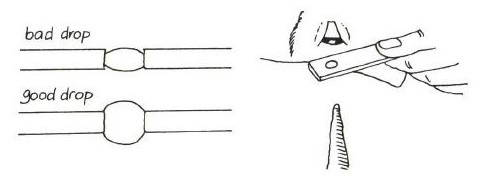
\includegraphics[width=8cm]{./img/vso/water-drop.jpg}
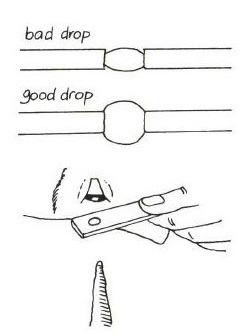
\includegraphics[width=0.45\textwidth]{./img/vso/water-drop-2.jpg}
\end{center}

\section{Slides}
A slide and even cover slip may be made from the same plastic water bottles, although being hydrophobic they will not have the same properties of glass when making wet mounts. Improvise a method for securing the punctured plastic over the slide; ideally the vertical spacing can be closely adjusted to focus.
\begin{center}
%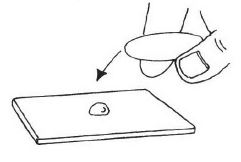
\includegraphics[width=4cm]{./img/vso/slide-cover-slip.jpg}
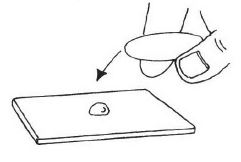
\includegraphics[width=0.45\textwidth]{./img/vso/slide-cover-slip.jpg}
\end{center}

\section{Backlighting}
On a bright day, there may not be any need for additional lighting, but in most classrooms the image will be too dim to be easily seen. The sun is a powerful light source, though not always convenient. Flashlights are generally inexpensive and available; many cell phones have one built in the end. To angle the light into the slide, find either a piece of mirror glass, wrinkle-free aluminum foil, the metalized side of a biscuit wrapper, etc.

Experiment with a variety of designs to see what works best given the materials available to your school. If you use a slide of onion cells stained with iodine solution
%(see \nameref{cha:sourcesofchemicals}, p.~\pageref{cha:sourcesofchemicals})
, your students should be able to see cell walls and nuclei.

\vfill
\columnbreak

\section{Simple Microscopes and \hfill \\ Magnifiers}

\subsection{Clear-Container Magnifiers}
\begin{center}
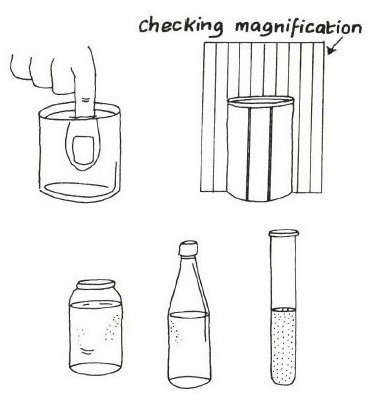
\includegraphics[width=0.4\textwidth]{./img/vso/container-microscope-2.jpg}
\end{center}

Any of these containers filled with water will make good magnifiers.

\subsection{Simple Microscope}
\begin{center}
%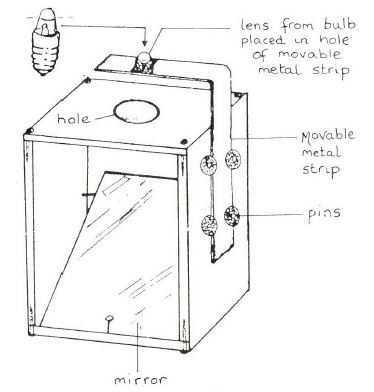
\includegraphics[width=0.49\textwidth]{./img/source/simple-microscope.jpg}
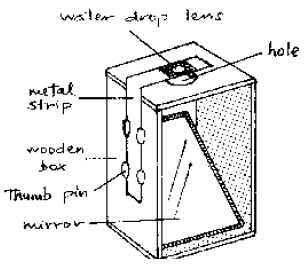
\includegraphics[width=0.49\textwidth]{./img/source/simple-microscope-2.png}
\end{center}

Construct a small wooden box from plywood as
shown (or use a small cardboard carton such as
a light bulb box). Make a round hole of 2 cm
diameter, at the top. Fit a small mirror (glass or
polished metal) in the box, angled to reflect light
up through the hole. Make a small hole (about 6
mm) in a strip of metal. Remove the round top
from a pen-torch bulb and secure it in the strip
using adhesive tape. Carefully cut off the tape
where it may cover the lens. Bend the strip, then
fix it to the side of the box, so that it can be
moved up and down. Drawing pins or nails
could be used for this. The object is focused by
moving this strip. Note the eye should be placed
as near as possible to the lens when viewing.

\vfill
\columnbreak

\subsection{Simple Compound \hfill \\ Microscope}
\begin{center}
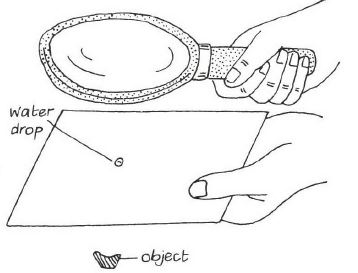
\includegraphics[width=0.4\textwidth]{./img/vso/compound-microscope.jpg}
\end{center}

\begin{itemize*}
\item Using 2 lenses together allows much greater magnification. 
\item Use a hand lens to make a water drop into a more powerful magnifier. 
\item Try using a hand lens with a lens from a torch bulb to make another simple compound microscope.
\end{itemize*}


\subsection{Card Bridge Microscope}
\begin{center}
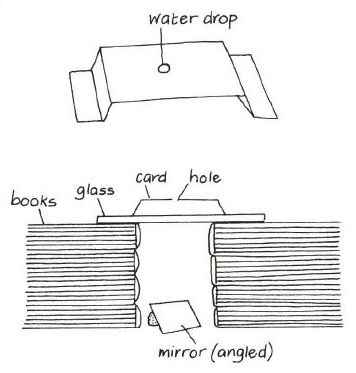
\includegraphics[width=0.4\textwidth]{./img/vso/card-microscope.jpg}
\end{center}

\begin{itemize*}
\item Place a water drop in the card `bridge'. 
\item Place this on a sheet of glass as shown. 
\item Place the object you are looking
at on the glass. This
arrangement is most suitable
for thin items, e.g. sections of leaves. 
\item Experiment with the angle of
the mirror so that light shines
up through the specimen.
\item Use this arrangement with a
hand lens to produce a
compound microscope.
\end{itemize*}

\vfill

\end{multicols}

% Part 5 - NECTA Practicals
\settocdepth{section} % Now we want to show up to the section level in the ToC
\part{NECTA Practicals} \index{Practicals} \index{NECTA Practicals|see{Practicals}}

\chapter{Biology Practicals} \index{Practicals! Biology}

\section{Introduction to Biology Practicals} 

\subsection{Format}

%Until 2008, NECTA biology practicals contained three questions. Question 1 was required, and was a food test. Students then chose to answer either question 2 or question 3. One of these questions was usually classification.
%
%The format changed in 2008. Now, the practical contains two questions, and both are required. Food test and classification remain the most common questions, but sometimes only one of these two topics is on a given exam. The second question may cover one of a variety of topics, including respiration, transport, coordination, photosynthesis, and movement.
%
%Each question is worth 25 marks.

\subsubsection{Biology Practical Format}

The format of the Biology practical exam was revised in 2011 to keep up with the 2007 updated syllabus. As such, there will be no further Alternative to Practical exams, pending approval from the Ministry of Education.

The Biology practical has 2 questions and students must answer both. Question 1 can come from any of the following topics: Nutrition, Movement, Transport of Living Things, Respiration, Reproduction, Coordination, Regulation or Growth. Question 2 is on Classification of Living Things. Each question is worth 25 marks, and students have 2$\frac{1}{2}$ hours to complete the exam.

\subsubsection{Biology 1 Theory Format}
The theory portion of the Biology exam comprises 100 marks, while the practical carries 50 marks. A student's final grade for Biology is thus found by taking her total marks from both exams out of 150.

The theory exam for Biology contains 13 questions over 3 sections. Section A has 2 questions worth 10 marks each.  Section B has 8 short answer questions, each having two items. This section weighs a total of 60 marks, and the mark allocation for individual questions is indicated at the end of each question. Section C has 3 long answer\slash essay questions, though students only need to answer 1 of them. The answer must be comprehensive and include as many points as possible. It is worth 20 marks.

\paragraph{Note} This information is current as of the time of publication of this manual. Updated information may be obtained by contacting the Ministry of Education. 

\subsection{Notes for Teachers}

\subsubsection{NECTA Advance Instructions}
Advance instructions are given to teachers at least one month before the date of the exam, as well as 24 hour advance instructions, to enable them to prepare apparatus, equipment and materials required for the examination.

%[tips for identifying practicals from advance instructions, example advance instructions?]

%\subsubsection{Words of Advice}

%\subsection{NECTA Marking Information}
%[how NECTA marks the practicals, highlight most important parts]

\subsection{Common Practicals}
\begin{description}
\item[Food Tests]{test a food solution for starch, sugars, fats, and protein}
\item[Classification]{name and classify specimens, then answer questions about their characteristics}
\item[Respiration]{use lime water to test air from the lungs for carbon dioxide}
\item[Transport]{investigate osmosis by placing leaf petioles or pieces of raw potato in solutions of different solute concentrations}
\item[Photosynthesis]{test a variegated leaf for starch to prove that chlorophyll is necessary for photosynthesis}
\item[Coordination]{students look at themselves in the mirror and answer questions about the sense organs they see}
\item[Movement]{name bones and answer questions about their structure and position in the body}
\end{description}

\paragraph{Note} These are the most common practicals, but they are not necessarily the only practicals that can occur on the national exam. Food tests and Classification are by far the most common, but there are many eligible topics. Be sure to regularly look through \nameref{cha:past-papers-bio} (p.~\pageref{cha:past-papers-bio}) to get an idea of the kind of questions that can occur.

%==============================================================================
\section{Food Tests} \index{Practicals! Biology! food tests} \index{Food tests}

In this practical, students test a solution of unknown food substances for starch, protein, reducing sugars, non-reducing sugars, and lipids. They record their procedure, observation, and conclusions, then answer questions about nutrition and the digestive system.\\

\noindent This section contains the following:
\begin{itemize}
\item{Preparation of Chemical Solutions}
\item{Preparation of Food Solutions}
\item{Performing the Food Tests}
\item{Examination Room}
\item{Student Report}
\item{Sample Food Test Practical}
%\item{Sample Food Test Solutions}
\end{itemize}

\subsection{Preparation of Chemical Solutions}
Always make sure the chemicals work before performing the food tests with students.

\subsubsection{Benedict's Solution} \index{Benedict's solution! for food tests}
This solution can be bought at a chemical store already prepared or you can make it yourself.\\

\textbf{Using Sodium Carbonate:}
\begin{itemize*}
\item Add about 1 L of water to a plastic bottle.
\item Add 5 spoons of sodium carbonate (NaCO$_3$).
\item Add 3 spoons of citric acid.
\item Add one spoon of copper sulphate.
\end{itemize*}

\textbf{Using Bicarbonate of Soda:}
\begin{itemize*}
\item Add 1 L of water to a cooking pot.
\item Add a box (70 g) of bicarbonate of soda.
\item Boil the mixture for 5-10 minutes. This makes sodium carbonate.
\item Let cool and transfer to a plastic water bottle.
\item Add 3 spoons of citric acid.
\item Add one spoon of copper sulphate. Cap and shake to mix.
\end{itemize*}

\noindent Label as: BENEDICT'S SOLUTION FOR FOOD TESTS

\noindent The solution may be stored in any plastic or glass bottle and will keep indefinitely.

\subsubsection{Copper (II) Sulphate} \index{Copper sulphate! for food tests}
\begin{itemize*}
\item Add one spoon of copper (II) sulphate to a 1.5 L bottle.
\item Add 1 L of water and shake until chemicals are fully dissolved.
\end{itemize*}

\noindent Label as: 1\% COPPER (II) SULPHATE SOLUTION FOR FOOD TESTS

\noindent The solution may be stored in any plastic or glass bottle and will keep indefinitely.

\subsubsection{Iodine Solution} \index{Iodine solution! for food tests}
Make sure to use iodine tincture from a pharmacy. The tincture must not contain ethanol\slash alcohol\slash spirit.

\begin{itemize*}
\item Add 1 part iodine tincture to 10 parts water. Example: In a 500 mL bottle, add 40 mL iodine tincture, then and 400 mL of water.
\item Cap the bottle and shake.
\end{itemize*}

\noindent Label as: IODINE SOLUTION FOR FOOD TESTS

\noindent The solution may be stored in any plastic or glass bottle and will keep indefinitely.

\subsubsection{Dilute NaOH} \index{Sodium hydroxide! for food tests}
\begin{itemize*}
\item Using a PLASTIC teaspoon, add one level teaspoon of NaOH to a 500 mL water bottle. Caustic soda (NaOH) reacts with metal. DO NOT TOUCH.

\emph{SAFETY NOTE: Prepare about 100 mL of citric acid or ethanoic acid solution to neutralize sodium hydroxide spills on skin or lab tables. One spoon of citric acid in 100 mL of water is suitable. Ethanoic acid solutions are sold in stores as vinegar.}

\item Add 250 mL of water.

\emph{SAFETY NOTE: This reaction can cause the solution to become very warm. Avoid chemical burns by wearing gloves.}

\item Cap well and shake. This makes 1 M sodium hydroxide solution.
\end{itemize*}

\noindent Label as: 1 M SODIUM HYDROXIDE SOLUTION FOR FOOD TESTS (CORROSIVE)

\noindent The solution will react with carbon dioxide in the air if not well sealed. Do not store in glass bottles with glass stoppers as these will stick. The solution may be stored in plastic bottles indefinitely.


\subsubsection{Dilute Acid} \index{Hydrochloric acid! for food tests} \index{Citric acid! for food tests}
Your school may have dilute hydrochloric acid or you may have to make it yourself.\\

\textbf{Using Hydrochloric Acid (HCl):}
\begin{itemize*}
\item Add 1 part HCl to 9 parts water. Example: In a 1.5 L water bottle, add 900 mL of water, then add 100 mL of HCl.
\item Shake well.
\end{itemize*}

\textbf{Using Citric Acid:}
\begin{itemize*}
\item Add 500 mL of water to a 1 or 1.5 L water bottle.
\item Add 5 spoons of citric acid.
\item Cap well and shake. This makes 0.5 M citric acid.
\end{itemize*}

\noindent Label as: 0.5 M CITRIC ACID FOR FOOD TESTS

\noindent The solution may be stored in any plastic or glass bottle and will keep indefinitely.

\subsubsection{Sudan III Solution} \index{Sudan III solution! for food tests}
Using Sudan III solution takes a long time to show results. It may be replaced by iodine tincture solution for the lipids test.

\begin{itemize*}
\item Combine 0.5 g of Sudan III powder with 100 mL of 70\% ethanol solution (30 mL water and 70 mL ethanol).
\item Place the solution in a warm water bath to help the Sudan III dissolve.
\item Filter to remove any remaining solid.
\end{itemize*}

\noindent Label as: SUDAN III SOLUTION FOR FOOD TESTS

\noindent The solution may be stored in any plastic or glass bottle and will keep indefinitely.


\subsection{Preparation of Food Solutions}
For the NECTA and mock exams you may have to set up the food test solutions. The instructions will tell you which ones you'll need to prepare in order to make `Solution X.' Solution X consists of a mixture of at least 3 of the different food substances and is given to each student in at least 3 test tubes. Make sure food solutions are well-dissolved and colorless so that students don't know what is in the mixture. You don't need to measure the ingredients, but make sure to test the solutions before the practical.

\subsubsection{Reducing sugar}
Use glucose powder and dissolve in water. Make sure the substance is fully dissolved so that students don't know what is in the mixture.

\subsubsection{Non-reducing sugar}
Use sugar and dissolve in water. Make sure the substance is fully dissolved so that students don't know what is in the mixture.

\subsubsection{Lipids}
Mix sunflower oil with water. Shake immediately before use. Sunflower oil is best since it is liquid at room temperature.

\subsubsection{Protein}
Mix an egg white with water.

\subsubsection{Starch}
Save the water you use to boil potatoes, rice, or pasta. Make sure to remove the bits of food. You can also just mix flour in water, but it would be obvious.


\subsection{Performing the Food Tests}

\subsubsection{Reducing Sugars Test}
\begin{itemize*}
\item Add a small amount of Benedict's solution to the food solution. 
\item Boil the solution and allow it to cool. Observe the colour changes from blue to green, yellow, then deep orange\slash brick red precipitate if reducing sugars are present.
\end{itemize*}
Always do the reducing sugars test first because a non-reducing sugar will always test positive for a reducing sugar.

\subsubsection{Non-reducing Sugars Test}
\begin{itemize*}
\item Add a small amount of dilute acid (HCl) to the solution. 
\item Boil the solution for about 30 seconds and allow it to cool. 
\item Add a small amount of NaOH to the solution and shake.
\item Add a small amount of Benedict's solution and boil. 
\item Allow the solution to cool and observe as the solution changes from green to yellow, then to deep orange\slash brick red precipitate if non-reducing sugars are present.
\end{itemize*}

\subsubsection{Lipids Test}
\begin{itemize*}
\item Add a small amount of Sudan III or iodine solution to the food solution and shake. 
\item A red ring will form at the top of the test tube if lipids are present.
\end{itemize*}
Using Sudan III colours the whole solution red whether it contains lipids or not. Use iodine solution to get a more distinct result.

\subsubsection{Protein Test}
\begin{itemize*}
\item Add an \emph{equal} amount of sodium hydroxide (NaOH) to the solution and shake. 
\item Add a small amount of copper (II) sulphate to the solution and shake.
\item Observe the solution turn violet\slash purple in colour if protein is present.
\end{itemize*}

\subsubsection{Starch Test}
\begin{itemize*}
\item Add a small amount of iodine solution to the food solution.
\item Observe the solution turn blue-black in colour if starch is present.
\end{itemize*}


\subsection{Examination Room}
The NECTA practical exam is done in the school's lab or any other suitable room. Heat sources (jiko, etc.) should be spread evenly in the exam room so that students don't have to go far to heat their test tubes; this also cuts down on cheating. Spread students out and distribute supplies as you see fit.\\

\noindent \textbf{Each student gets:}
\begin{itemize*}
\item[-] 3 or more test tubes (to carry out 5 tests)
\item[-] A beaker containing Solution X
\item[-] A test tube rack (or a cut out water bottle with sand to hold the tubes)*
\end{itemize*}
* Students may share the racks, but shouldn't share the cut out bottles\\

\noindent \textbf{Each station should have:}
\begin{itemize*}
\item[-] Copper II sulphate
\item[-] Water
\item[-] Dilute acid (HCl, etc.)
\item[-] Dilute base (sodium hydroxide)
\item[-] Iodine solution
\item[-] Sudan III solution (can be replaced by iodine solution)
\item[-] Benedict's solution
\end{itemize*}

\subsection{Student Report}
Food test data is recorded in a table containing four columns: Test for, Procedure, Observation and Inference.

Students should write the Procedure using the passive voice in the past tense. For example, ``A small amount of Benedict's solution was added to the solution. Then the solution was boiled and allowed to cool.''

In the Observation column, the student should write what they observed using the past tense and passive voice. For example, ``A violet colour was observed.''

In the Inferences column, the students should write what they saw in the past tense and passive voice. For example, ``Reducing sugars were not (or were) present.''

Note that every column is worth marks on the exam. Even if students fail to do the food tests correctly, they can still get marks for writing what they are testing for and what the procedure should be.

An example of a completed food test results table is given below. Assume the solution contains proteins, reducing sugars, non-reducing sugars and starch.

\begin{center}
\begin{tabular}{|p{3cm}|p{5cm}|p{3cm}|p{3cm}|} \hline
\multicolumn{1}{|c|}{\textbf{Food Tested}}&\multicolumn{1}{c|}{\textbf{Procedure}}&\multicolumn{1}{c|}{\textbf{Observation}}&\multicolumn{1}{c|}{\textbf{Inference}} \\ \hline
Lipids & A few drops of Sudan III solution (or iodine solution) were added to solution X. The solution was shaken and allowed to stand. & A red ring did not form at the surface. & Lipids were not present.\\ \hline
Proteins & An equal amount of NaOH was added to solution X and shaken. A few drops of copper (II) sulphate were added to solution X and shaken again. & A violet colour was observed. & Proteins were present.\\ \hline
Reducing sugars & A small amount of Benedict's solution  was added to solution X. The solution was heated and allowed to cool. & A brick red precipitate was observed. & Reducing sugars were present.\\ \hline
Non-reducing sugars & A small amount of dilute acid was added to solution X. The solution was heated and allowed to cool. Then a small amount of NaOH solution was added, and the solution was shaken. Finally, a small amount of Benedict’s solution was added. The solution was boiled and let cool. & The solution changed from green to yellow, then to a deep orange\slash brick red precipitate. & Non-reducing sugars were present.\\ \hline
Starch & A few drops of iodine solution were added to solution X and shaken. & A blue-black colour was observed. & Starch was present.\\ \hline
\end{tabular}
\end{center}

\subsection{Sample Food Test Practical}
You have been provided with solution \textbf{B}. 

\begin{enumerate}
\item[(a)] Identify the food substances present in solution \textbf{B} by using the reagents provided. Tabulate your work as shown in the following Table:

\begin{center}
\begin{tabular}{|p{3cm}|p{3cm}|p{3cm}|p{3cm}|} \hline
\multicolumn{1}{|c|}{\textbf{Food Tested}}&\multicolumn{1}{c|}{\textbf{Procedure}}&\multicolumn{1}{c|}{\textbf{Observation}}&\multicolumn{1}{c|}{\textbf{Inference}} \\ \hline
&&& \\
&&& \\
&&& \\
&&& \\ \hline
\end{tabular} \\[10pt]
\end{center}

\item[(b)] For each food substance identified in 1(a);
\begin{enumerate}
\item[(i)] Name two common sources.
\item[(ii)] State their role in the body of human being.
\end{enumerate}
\item[(c)] The digestion of one of the identified food substance in 1(a) starts in the mouth.
\begin{enumerate}
\item[(i)] Name this food substance.
\item[(ii)] Identify the enzyme responsible for its digestion in the mouth.
\end{enumerate}
\item[(d)] The digestive system of human being has several parts.
\begin{enumerate}
\item[(i)] Name the part of digestive system in which most of digestion and absorption of food takes place.
\item[(ii)] Explain how the named part in (d) (i) is adapted for absorption of digested food substances.
\end{enumerate}
\end{enumerate}

\textbf{Additional Food Test Questions:}
See \nameref{cha:past-papers-bio} (p.~\pageref{cha:past-papers-bio}) for additional food test questions.

%\begin{enumerate*}
%\item[(e)] What is the function of each of the food substances in solution \textbf{B} to human beings? 
%\item[(f)] For each food substance identified, name the enzyme and end product of digestion 
%taking place in the:\\
%\begin{enumerate*}
%\item[(i)] Stomach
%\item[(ii)] Duodenum
%\end{enumerate*}
%\item[(g)] What deficiency diseases are caused by a lack of the identified food substances?
%\end{enumerate*}


%\subsection{Sample Food Test Solutions}



%\section{Food Tests}
%
%In this practical, students test a solution of unknown food substances for starch, protein, reducing sugars, non-reducing sugars, and fats\slash oils. They record their procedure, observation, and conclusions, then answer questions about nutrition and the digestive system.
%
%This section contains the following:
%\begin{itemize}
%\item{Preparation of test solutions}
%\item{Preparation of food solutions}
%\item{How to carry out food tests}
%\item{How to write a report}
%\item{Sample practical with solutions}
%\end{itemize}
%
%\subsection{Test for Starch}
%
%\subsubsection{Materials}
%\begin{itemize}
%\item{iodine tincture from the pharmacy (any brand)}
%\item{tap or clean river water}
%\end{itemize}
%
%\subsubsection{Procedure to make 400~mL}
%\begin{enumerate}
%\item{40~mL of iodine tincture to a 500~mL plastic water bottle.}
%\item{Add about 400~mL of water.}
%\item{Cap the bottle and shake.}
%\item{Use a permanent pen to label the bottle:\\
%IODINE SOLUTION FOR FOOD TESTS}
%
%The solution may be stored in any plastic or glass bottle and will keep indefinitely.
%\end{enumerate}
%
%\subsection{Test for protein}
%
%The best test for protein is the Biuret test. This requires two solutions: 1\% \ce{CuSO4} and 1~M \ce{NaOH}.
%
%\subsubsection{Materials}
%\begin{itemize}
%\item{copper sulfate}
%\item{sodium hydroxide}
%\item{tap or clean river water}
%\end{itemize}
%
%\subsubsection{Procedure to make 1~L copper sulfate solution}
%\begin{enumerate}
%\item{Use a small metal or plastic spoon (tea size) to transfer one level spoon of copper sulfate into a 1 or 1.5~L water bottle.}
%\item{Add about one liter of water. The amount does not have to be exact.}
%\item{Cap the bottle and shake until the copper sulfate has completely dissolved.}
%\item{Use a permanent pen to label the bottle:\\
%1\% Copper (II) Sulfate Solution\\
%For food tests}
%\end{enumerate}
%
%The solution may be stored in any plastic or glass bottle and will keep indefinitely.
%
%\subsubsection{Procedure to make 250~mL of sodium hydroxide solution}
%\begin{enumerate}
%\item{Use a small PLASTIC spoon (tea size) to transfer one level spoon of sodium hydroxide into a 500~mL water bottle. Caustic soda (sodium hydroxide) reacts with metal. DO NOT TOUCH.
%
%\textit{SAFETY NOTE: prepare about 100~mL of citric acid or ethanoic acid solution to have available to neutralize sodium hydroxide spills on skin or lab tables. One spoon of citric acid in about 100~mL of water is a suitable concentration. Ethanoic acid solutions of the proper concentration are sold in food shops as vinegar.}
%
%}%item
%
%\item{Add about 250~mL of water to the bottle. In the new 500~mL Maji Africa bottles, this is the first straight line above the curving lines. The addition of water to sodium hydroxide gets HOT.}
%\item{Cap the bottle very well and shake to mix.}
%\item{Use a permanent pen to label the bottle:\\
%1~M SODIUM HYDROXIDE SOLUTION FOR FOOD TESTS\\
%CORROSIVE. Neutralize spills with weak acid solution.}
%\end{enumerate}
%
%The hydroxide solution will react with carbon dioxide in the air if the container is not well sealed. The solution should not be stored in glass bottles with glass stoppers for overnight or longer as these will stick. The solution may be stored in plastic bottles indefinitely.
%
%\subsection{Test for lipids}
%
%\subsubsection{Materials}
%\begin{itemize}
%\item{Provodine iodine tincture from the pharmacy -- the tincture must be without ethanol\slash alcohol\slash ``spiriti''}
%\item{tap or clean river water}
%\end{itemize}
%
%\subsubsection{Procedure to make 400~mL}
%See instructions for preparing iodine solution for Test for Starch above.
%
%\subsubsection{A note on theory}
%
%Many biology books call for a chemical called Sudan III to test for lipids. Sudan III is a bright red pigment that is much more soluble in oil than in water. For this reason, Sudan III solution is usually prepared using ethanol to bring the Sudan III pigment into the solution. In mixtures of oil and water, the oil separates and moves to the top. When shaken with Sudan III, this oil absorbs the Sudan III, turns red, and produces a ``red ring'' at the top of the test tube. However, the ethanol used to make Sudan III causes the water and oil to form an emulsion. In an emulsion, the oil is broken into very small particles and it takes a long time for this emulsion to break down and form an oil layer on the top. Hence testing with Sudan III takes a long time to show a clear result.
%
%Iodine is another coloured molecule that is more soluble in oil than in water. When a mixture of oil and water is shaken with iodine solution, the iodine moves to the oil layer, colouring it orange or red. This also gives the result of a ``red ring'' at the top of the test tube. To prevent an emulsion forming -- as happens with Sudan III -- it is very important to make iodine solution from pharmacy tincture that is without ethanol. Another benefit of using iodine is that while Sudan III is always red, iodine is uniquely yellow in water and red in oil, making the difference between positive and negative results easier to see. Because there is no ethanol in iodine solution, the result also comes much faster, usually within 10-20 seconds.
%
%Note that if the oil and water mixture settles before you transfer it to the test tube, there may be too little or too much oil in the test tube. Shake the food sample solution before taking each sample.
%
%\subsection{Test for reducing sugars with Benedict's solution}
%
%\subsubsection{Materials}
%\begin{itemize}
%\item{sodium carbonate (soda ash) if available, otherwise sodium hydrogen carbonate (bicarbonate of soda)}
%\item{citric acid}
%\item{copper sulfate}
%\item{tap or clean river water}
%\item{plastic water bottle with screw cap}
%\end{itemize}
%
%\subsubsection{Procedure to make 1~L using soda ash}
%Combine the following into the bottle in order, adding slowly:
%\begin{enumerate}
%\item{about 1~L water}
%\item{five spoons of sodium carbonate}
%\item{three spoons of citric acid}
%\item{one spoon of copper sulfate.}
%\end{enumerate}
%
%All measurements with the spoon should be level to ensure that the volume measured is consistent. The final solution should have a bright blue color.
%
%\subsubsection{Procedure to make 500~mL using sodium hydrogen carbonate}
%\begin{enumerate}
%\item{Add 500~mL of water to a cooking pot.}
%\item{Add a box (70~g) of bicarbonate of soda to the water.}
%\item{Heat the pot on a stove until boiling. Let boil for ten minutes.}
%\item{Remove the pot from the stove and let cool. When cool, transfer the liquid to a plastic water bottle.}
%\item{Slowly add one and a half spoons of citric acid.}
%\item{Add half a spoon of copper sulfate. Cap and shake to mix.}
%\end{enumerate}
%
%Label the final solution:
%
%\begin{center}	
%BENEDICT'S SOLUTION FOR FOOD TESTS.
%\end{center}
%
%The solution may be stored in any plastic or glass bottle and will keep indefinitely.
%
%\subsection{Test for non-reducing sugar}
%
%\subsubsection{Materials}
%\begin{itemize}
%\item{Benedict's solution, above}
%\item{1M sodium hydroxide solution, above under protein test}
%\item{citric acid}
%\item{tap or clean river water}
%
%To perform this test, students first test their sample with Benedict's solution to eliminate the possibility of a reducing sugar. Then, they must use an acid solution to hydrolyze any non-reducing sugars and then a base solution to neutralize the sample solution. Then the students perform again the test for non-reducing sugars.
%
%\subsubsection{Procedure to make 500~mL of acid solution}
%\begin{enumerate}
%\item{Put 500~mL of water into a plastic water bottle.}
%\item{Add five spoons of citric acid.}
%\item{Cap the bottle very well and shake to mix.}
%\item{Use a permanent pen to label the bottle:\\
%0.5~M CITRIC ACID FOR FOOD TESTS}
%\end{enumerate}
%
%The solution may be stored indefinitely in any plastic or glass container.
%
%\subsection{Preparation of Food Sample Solutions}
%
%Try to make food solutions colorless so that students cannot guess what is in them, and so that they can see the colors that form during food tests. You do not need to measure the ingredients of the solution, but make sure to test solutions before the practical.
%
%\subsubsection{Starch solution}
%The easiest solution is the water left from boiling pasta or potatoes. If you have been only ugali and rice lately, add some wheat or corn flour to boiling water. Let cool. Decant the solution or filter it with a tea filter to remove the largest particles. If you are in a hurry, you can also just mix flour with cold water, but then it will be obvious that flour is present.
%
%\subsubsection{Lipids}
%Add cooking oil to water. Shake immediately before use. Sunflour oil is best – avoid fats that solidify near room temperature.
%
%\subsubsection{Protein solution}
%Combine egg whites with water. If you do not have egg whites, you can use fresh or powder milk, although this will give the solution a white color and add a reducing sugar (lactose). The water used in boiling beans also contains some protein, but it may not be enough to see a color change.
%
%\subsubsection{Reducing sugar}
%The easiest is to buy glucose powder from a shop and dissolve it in water. You can also grind pieces of onion with water and filter the resulting solution.
%
%\subsubsection{Non-reducing sugar}
%Dissolve sugar in water. Table sugar is sucrose, a non-reducing sugar.
%
%\subsection{How to Carry Out Food Tests}
%
%\subsubsection{Starch}
%Add a few drops of iodine to the solution and shake well. A blue-black color forms if starch is present
%
%\subsubsection{Lipids}
%Add a few drops of iodine to the solution and shake well. A red ring will form at the top of the test tube is lipids are present.
%
%You can also have your students do the grease spot test -- rub a drop of solution onto a piece of paper, and let dry. A translucent spot forms if fat is present. This test is great for its simplicity, but is not used on national exams.
%
%\subsubsection{Protein (Biuret test)}
%Add a few drops of 1~M \ce{NaOH} to the solution and shake well. Then add a few drops of 1\% \ce{CuSO4} solution and shake. A violet color forms if protein is present. Sometimes the color takes a minute or two to appear. 
%
%Some textbooks may recommend using Millon's reagent to test for protein. This reagent contains mercury, which is extremely poisonous and should never be handled by students.
%
%The purple colour from a positive test is the result of a complex between four nitrogen atoms and the copper (II) ion. Specifically, these nitrogen atoms are all part of peptide bonds. These peptide bonds are adjacent on a protein, either two from one protein and two from another, or two from one part of a protein and two from another part of the same protein.
%
%\subsubsection{Reducing sugar}
%Place some food solution in a test tube, and add an equal volume of Benedict’s solution. Heat to boiling, then let cool. A brick red or orange precipitate forms if a reducing sugar is present.
%
%Benedict's solution contains aqueous copper (II) sulphate, sodium carbonate, and sodium citrate. The citrate ions in Benedict's solution complex the copper (II) ions to prevent the formation of insoluble copper (II) carbonate. In the presence of a reducing sugar, however, the copper (II) ions are reduced to copper (I) ions which form a brick red precipitate of copper (I) oxide. The oxygen in the copper (I) oxide come from hydroxide; the purpose of the sodium carbonate is to provide this hydroxide by creating an alkaline environment.
%
%Normally, sugar molecules form five or six member rings and have no reducing properties. In water, however, the rings of some sugar molecules can open to form a linear structure, often with an aldehyde group at one end. These aldehyde groups react with copper (II) to reduce it to copper (I). Sugars that do not have an aldehyde group in the linear structure or that are not able to open are not able to reduce copper (II) ions and are thus called non-reducing sugars. Students do not need to understand this chemistry for their exam, but they may ask about what is happening in the reaction.
%
%\subsubsection{Non-reducing sugar}
%Do the test for a reducing sugar using Benedict's solution. Notice that no reaction occurs. Add a few drops of citric acid solution to the solution, then heat to boiling. Let solution cool. Add a few drops of 1~M \ce{NaOH}, and shake well. Then, add some Benedict’s solution (equal in volume to the liquid in the test tube). Boil the solution, and let it cool. A brick red or orange precipitate forms if a non-reducing sugar is present.
%
%This experiment will also test positive for all reducing sugars. Therefore it is important to first perform the test for reducing sugars before considering this test. If the test for reducing sugars is positive, there is no reason to perform the test for non-reducing sugars -- the conclusion will be invalid.
%
%Non-reducing sugars are a misnomer, that is, their name is incorrect. This test does not test for any sugar that is not reducing. Rather, this is a test for any molecule made of multiple reducing sugars bound together, such as sucrose or starch. When these polysaccharides are heated in the presence of acid, they hydrolyse and release monosaccharides. The presence of these monosaccharides is then identified with Benedict's solution.
%
%The purpose of the sodium hydroxide is to neutralize the citric acid added for hydrolysis. If the citric acid is not hydrolysed, it will react with the sodium carbonate in Benedict's solution, possibly making the solution ineffective.
%
%\subsection{How to Write a Report}
%Food test data is reported in a table containing four columns: test for, procedure, observation, and inference. With the exception of the `test for' column, data should be reported in full sentences written in past tense. The procedure should also be in passive voice. No, this is not the way professional scientists write. However, students here must use passive voice to get marks on the national exam.
%
%Note that every column is worth marks on the exam. Even if students fail to do the food tests correctly, they can still get marks for writing what they are testing for and what the procedure should be.
%
%See the sample practical below for an example of a report.
%
%\subsection{Sample Food Test Practical}
%
%You have been provided with Solution K. Carry out food test experiments to identify the food substances present in the solution.
%\begin{enumerate}
%
%\item{Record your experimental work as shown in the table below.}
%
%\begin{center}
%\begin{tabular}{| c | c | c | c |}
%\hline
%Test for & Procedure & Observations & Inferences\\ \hline
%Protein & & & \\ \hline
%Starch & & & \\ \hline
%Lipids & & & \\ \hline
%Reducing sugars & & & \\ \hline
%Non-reducing sugars & & & \\ \hline
%\hline
%\end{tabular}
%\end{center}
%
%\item{Suggest two natural food substances from which solution K might have been prepared.}
%\item{What is the function of each of the food substances in solution K to human beings?}
%\item{For each food substance identified, name the enzyme and end product of digestion taking place in the:}
%\begin{enumerate}
%\item{Stomach}
%\item{Duodenum}
%\end{enumerate}
%\item{What deficiency diseases are caused by a lack of the identified food substances?}
%\end{enumerate}
%
%\subsection{Sample Practical Solutions}
%(Assume Solution K contains protein and starch.)
%
%\item{The results were as follows}
%
%\begin{center}
%\begin{tabular}{| c | c | c | c |}
%\hline
%Test for & Procedure & Observations & Inferences\\ \hline
%Protein & 
%A few drops of NaOH solution & A violet color & Protein was present. \\
%& were added to Solution K. & was observed. &\\
%& The solution was shaken.& & \\
%& Then a few drops of & &\\
%& \ce{CuSO4} solution were & & \\
%& added to Solution K, and the & &\\
%& solution was shaken again. & &\\ \hline
%Starch & A few drops of iodine & A blue-black color & Starch was present. \\
%& solution were added & was observed. & \\
%& to Solution K, and & & \\
%& the solution was shaken. & & \\ \hline
%Lipids & A few drops of Sudan III & A red ring did not & Fats/oils were absent. \\
%& solution (or iodine solution) & form at the surface. & \\
%& were added to Solution K. & & \\
%& The solution was shaken & & \\ 
%& and then allowed to stand. & & \\ \hline
%Reducing & A small amount of Benedict’s & There was no & Reducing sugars  \\
%sugars & solution was added & precipitate & were absent.\\
%& to Solution K. & & \\
%& The solution was boiled & & \\
%& and allowed to cool. & & \\ \hline
%Non- & A small amount of dilute & There was no & Non-reducing \\
%reducing & acid was added to & precipitate.& sugars were absent.\\
%sugars & Solution K. The solution & &\\
%& was boiled and allowed to cool. & & \\
%& Then a small amount of & & \\
%& NaOH solution was added, & & \\
%& and the solution was shaken. & & \\
%& Finally, a small amount of & & \\
%& Benedict’s solution was added. & & \\
%& The solution was boiled & & \\
%& and let cool. & &\\ \hline
%\hline
%\end{tabular}
%\end{center}
%
%\item{Solution K could have been prepared from egg and maize. \textit{(Note: Any non-processed food containing protein or starch is correct here.)}}
%\item{Starch provides energy to the body. Proteins are used in growth and tissue repair.}
%
%\begin{center}
%\begin{tabular}{| c | c | c | c |}
%\hline
%Food Substance & Location & Enzyme & End Product of Digestion\\ \hline
%Protein & Stomach & \textit{Pepsin} & Polypeptides \\ \hline
%Protein & Duodenum & \textit{Trypsin} & Amino acids \\ \hline
%Starch & Duodenum & \textit{Pancreatic amylase} & Maltose \\ \hline
%\hline
%\end{tabular}
%\end{center}
%
%\item{A deficiency of protein causes kwashiorkor. A deficiency of starch causes marasmus.}
%\end{itemize}

%==============================================================================
\section{Classification} \index{Practicals! Biology! classification} \index{Classification}

The classification practical requires students to identify specimens of animals, plants, and fungi. The students must write the common name, kingdom, phylum, and sometimes class of each specimen. They also answer questions about the characteristics and uses of the specimens.

This section contains the following:
\begin{itemize}
\item{Common specimens}
\item{Where to find specimens}
\item{Storage of specimens}
\item{Sample practical with solutions}
\item{Additional classification questions}
\end{itemize}

\subsection{Common Specimens}
\begin{description}
\item[Fungi]{Mushroom, yeast, bread mold}
\item[Plants]{Fern, moss, bean plant, bean seed, maize plant, maize seed, pine tree, cactus, sugar cane, Irish potato1, cypress tree, acacia tree, hibiscus leaf, cassava}
\item[Animals]{Millipede, centipede, grasshopper, lizard, tilapia (fish)3, scorpion, frog, tapeworm, liver fluke, cockroach, spider}
\end{description}

\subsection{Where to Find Specimens}
\begin{itemize}
\item{Start collecting specimens several months before the NECTA exams, as some specimens can be hard to find in the dry season.}
\item{Ask your students to bring specimens! Students are especially good at finding insects and other animals. You can even find primary school children to gather insects such as grasshopper and millipedes.}
\item{Ferns, hibiscus, pines, and cypresses are used in landscaping. Try looking near nice hotelis or guestis. Ferns should have sori (sporangia) on the underside of their leaves.}
\item{Moss often grows near water tanks and in shady corners of courtyards. It is hard to find in the dry season.}
\item{Sugarcane, Irish potato, cassava, tilapia, bean seeds, and maize seeds can be found at the market. Yeast is available at shops.}
\item{Mushrooms are hard to find in the dry season. However, they are available at grocery stores in large cities, and you may be able to find dried mushrooms at the market. You can also collect mushrooms in the rainy season and dry them yourself.}
\item{Tapeworms and liver flukes may be acquired from butchers. Find out where livestock is slaughtered and ask the butchers to look for worms (minyoo). Liver flukes are found in the bile ducts inside the liver, while tapeworms are found in the intestines. You can also try going to a livestock fair\slash market (mnada) or talking to the local meat inspector (mkaguzi wa nyama).}
\item{Grow your own bread mold. Just put some bread in a plastic bag and leave it in a warm place. But do it ahead of time -- it can take two weeks to obtain bread mold with visible sporangia.}
\end{itemize}

\subsection{Storage of Specimens}
\begin{itemize}
\item{Insects and mushrooms can be dried and stored in jars. However, they become brittle and break easily.}
\item{A 10\% solution of formaldehyde is the best way of storing specimens. Formaldehyde is often sold as a 40\% solution. It should be stored in glass jars and out of the sun. Check specimens periodically for evaporation. Formaldehyde works because it is toxic; handle carefully.}
\item{In a pinch, a 70\% solution of ethanol can also be used to store insects, lizards, and worms. However, specimens sometimes decay in ethanol.}
­­\end{itemize}

\subsection{Sample Classification Practical}

You have been provided with specimens L, M, N, O, and P.
\begin{enumerate}
\item{Identify the specimens by their common names.}
\item{Classify each specimen to the phylum level.}	
\item{Further classification:}
\begin{enumerate}
\item{Write the classes of specimens L and M.}
\item{List two observable differences between specimens L and M.}
\end{enumerate}
\item{Explain why specimen P cannot grow taller.}
\item{Write down two distinctive characteristics of the phylum to which specimen O belongs.}
\item{Reproduction:}
\begin{enumerate}
\item{List the modes of reproduction in specimens M and N.}
\item{What are two differences between these modes of reproduction?}
\end{enumerate}
\end{enumerate}

\subsection{Sample Practical Solutions}

\begin{enumerate}

\item{Common names of specimens:}
\begin{itemize}
\item{L: maize plant}
\item{M: bean plant}
\item{N: yeast}
\item{O: millipede}
\item{P: moss}
\end{itemize}


\item{Classifaction by kingdom and phylum:}

\begin{center}
\begin{tabular}{| c | c | c |}
\hline
Specimen & Kingdom & Phylym \\ \hline
L (maize plant) & Plantae & Angiospermophyta \\ \hline
M (bean plant) & Plantae & Angiospermophyta \\ \hline
N (yeast) & Fungi & Ascomycota \\ \hline
O (millipede) & Animalia & Arthropoda \\ \hline
P (moss) & Plantae & Bryophyta \\ \hline
\hline
\end{tabular}
\end{center}

\item{Further classification:}
\begin{itemize}
\item{Specimen L (maize plant): Class Monocotyledonae}
\item{Specimen M (bean plant): Class Dicotyledonae}
\item{Observable differences:}

\begin{center}
\begin{tabular}{| c | c | c |}
\hline
Specimen & Vein structure & Root structure \\ \hline
L (maize plant) & Parallel veins & Fibrous roots \\ \hline
M (bean plant) & Net veins & Tap roots \\ \hline
\hline
\end{tabular}
\end{center}

\textit{The answers to this question should be differences between monocots and dicots that the student can see by observing the plants with their naked eyes. Hence answers such as ``vascular bundles in a ring'' are not correct.}

\end{itemize}

\item{Specimen P (moss) cannot grow taller because it has no xylem and phloem. If it grew taller, it would not be able to transport food and water throughout the plant.}
\item{Characteristics of phylum Arthropoda:}
\begin{itemize}
\item{jointed legs}
\item{segmented body}
\item{exoskeleton made of chitin}
\end{itemize}
\item{Reproduction}
\begin{enumerate}
\item{Specimen M (bean plant) reproduces by sexual reproduction. Specimen N (yeast) reproduces by asexual reproduction.}

\begin{center}
\begin{tabular}{| c | c | c | c |}
\hline
Method & Genetic variation & Parents & Gametes \\ \hline
Asexual & There is no genetic & Requires one & No gametes  \\
reproduction & variation between offspring. & parent only. & are involved. \\ \hline
Sexual & There is genetic & Usually requires & Involves fusion  \\
reproduction & variation between offspring. & two parents. & of two gametes.\\ \hline
\hline
\end{tabular}
\end{center}

\end{enumerate}
\end{enumerate}

\subsection{Additional Classification Questions}
\begin{itemize}
\item{Identify specimen X, Y, and Z by their common names.}
\item{Classify specimens X, Y, and Z to the class level. (This means write the kingdom, phylum, and class.)}
\item{Write the observable features of specimen X.}
\item{List three observable differences\slash similarities between specimens X and Y.}
\item{State the economic importance of specimen X.}
\item{What characteristics are common among specimens X and Y?}
\item{Why are specimens X and Y placed in different classes\slash phyla\slash kingdoms?}
\item{Why are specimens X and Y classified under the same class\slash phylum\slash kingdom?}
\item{What distinctive features place specimen X in its respective kingdom\slash phylum\slash class?}
\item{How is specimen X adapted to its way of life?}
\item{Suggest possible habitats for specimens X and Y.}
\item{Which specimen is a primary producer\slash parasite\slash decomposer?}
\item{For mushroom, yeast, bread mold, grasshopper, moss, tilapia, liver fluke, and tapeworm: Draw and label a diagram of specimen X.}
\item{For tilapia: Draw a big and well-labeled diagram showing a lateral view of specimen X.}
\item{For maize and bean:}
\begin{itemize}
\item{Mention the type of pollination in specimen X [wind pollinated or insect pollinated].}
\item{How is specimen X adapted to this type of pollination?}
\item{Mention the type of germination [hypogeal or epigeal] in specimen X.}
\end{itemize}
\item{For bean seed:}
\begin{itemize}
\item{List three observable features of specimen X and state their biological importance.}
\item{Split specimen X into two natural halves. Draw and label the half containing the embryo.}
\end{itemize}
\item{For fern:}
\begin{itemize}
\item{Observe the underside of the leaves of specimen X}
\item{What is the name of the structures you have observed?}
\item{Give the function of the structures named above.}
\item{Draw specimen X and show the structures named above.}
\end{itemize}
\end{itemize}
%==============================================================================
\section{Respiration} \index{Practicals! Biology! respiration} \index{Respiration}

The purpose of this practical is to investigate the properties of air exhaled from the lungs. This section contains the following:

\begin{itemize}
\item{Limewater (properties and preparation)}
\item{Apparatus}
\item{Cautions and advice when using traditional materials}
\item{Sample practical with solutions}
\end{itemize}

\subsection{Limewater}
Limewater is a saturated solution of calcium hydroxide. It is used to test for carbon dioxide. When carbon dioxide is bubbled through limewater, the solution becomes cloudy. This is due to the precipitation of calcium carbonate by the reaction:

\ce{CO2_{(g)}} + \ce{Ca(OH)2_{(aq)}} $\longrightarrow$ \ce{CaCO3_{(s)}}

Limewater can be prepared from either calcium hydroxide or calcium oxide. Calcium oxide reacts with water to form calcium hydroxide, so either way you end up with a calcium hydroxide solution. Calcium oxide is the primary component in cement. Calcium hydroxide is available from building supply shops as \textit{chokaa}.

To prepare lime water, add three spoons of fresh \textit{chokaa} or cement to a bottle of water. Shake vigorously and then let stand until the suspended solids precipitate. Decant the clear solution. \textit{Chokaa} produces a solution much faster than cement.

The exact mass of calcium hydroxide or calcium oxide used is not important. Just check whether some calcium hydroxide remains undissolved at the end -- a sign that you have made a saturated solution.

Test limewater by blowing air into a sample with a straw. It should become cloudy. If it does not, then the concentration of \ce{Ca(OH)2} is too low.

\subsection{Apparatus}
Many books call for delivery tubes, test tubes, and stoppers. These are totally unnecessary. Add the limewater to any small clear container and blow into it with a straw.

\subsection{Cautions and Advice When Using Traditional Materials}
If you use a delivery tube and pass it through a rubber stopper, do not use a single-holed stopper. This is what the pictures on NECTA practicals suggest, but it is a terrible idea. A single-holed stopper has no space for air to escape. So when a student blows air into the solution, the pressure in the test tube increases. The high pressure air then pushes limewater up the straw into the student's mouth. Alternatively, the student blows the stopper out of the test tube. If you use a stopper, use a double-holed stopper so that the extra air has a place to escape.

Is a glass delivery tube stuck in a rubber stopper? Do not pull hard on it. Just soak the stopper in warm water for a few minutes. The rubber will soften and the tube will come out.

Are your test tubes and delivery tubes cloudy after the practical? Clean them with dilute acid. This will dissolve any calcium carbonate that has been deposited on the glass.

\subsection{Sample Respiration Practical}

You have been provided with Solution B in a test tube. Use a delivery tube to breathe (exhale) into the solution until its color changes. (See diagram below.) 

\begin{enumerate}
\item{What is the aim of this experiment?}
\item{What is Solution B?}
\begin{enumerate}
\item{What changes did you observe after breathing into Solution B?}	
\item{What can you conclude from these changes?}
\end{enumerate}
\item{Breathe out over the palm of your hand. What do you observe?}
\item{Breathe out over a mirror. What do you observe?}
\item{Using your observations in the three experiments above, list three properties of exhaled air.}
\item{Explain why exhaled air is different from inhaled air. Where do the substances you identified in exhaled air come from?}
\end{enumerate}

\subsection{Sample Practical Solutions}

\begin{enumerate}
\item{The aim of this experiment is to test exhaled air for carbon dioxide.}
\item{Solution B is limewater.}
\begin{enumerate}
\item{Solution B became cloudy (or milky).}
\item{Conclusion: exhaled air contains carbon dioxide.}
\end{enumerate}
\item{Air breathed out over the palm of the hand is warm.}
\item{Droplets of water condense on the mirror.}
\item{Conclusions:}
\begin{itemize}
\item{exhaled air contains carbon dioxide}
\item{exhaled air contains water}
\item{exhaled air is warm}
\end{itemize}
\item{Exhaled air contains the waste products of aerobic respiration. The carbon dioxide and water in exhaled air are products of respiration.}
\end{enumerate}

%==============================================================================
\section{Transport} \index{Practicals! Biology! transport} \index{Transport}

The purpose of this practical is to investigate osmosis by observing the changes in a leaf petiole placed in a hypotonic solution (water) and a hypertonic solution (water containing salt or sugar). 

This section contains the following:
\begin{itemize}
\item{Materials}
\item{Sample practical with solutions}
\item{Additional questions}
\end{itemize}

\subsection{Materials}
The petiole is the stalk which attaches a leaf to a branch. The papaya leaf petioles in this practical should be soft petioles from young leaves, not stiff petioles from older leaves. Cut the petioles into pieces, and give each student two pieces of about 6 cm in length. Cylinders cut from a raw potato  may be used instead of petioles.

The hypertonic solution may be made with by mixing either salt or sugar with water. The hypotonic solution is tap water.

\subsection{Sample Transport Practical}

\subsubsection{Instructions}

You have been provided with two pieces of a papaya leaf petiole, Solution A, and Solution B.
 
Use a razor blade to split the pieces of petiole longitudinally, up to a half of their length. You should have four strips at one end of each petiole, while the other end remains intact. 

Place one petiole in solution A, and place the other petiole in solution B. Let the petiole  sit for about ten minutes, then touch them to feel their hardness or softness.

Draw a sketch of each petiole after sitting in its respective solution for ten minutes.

Record your observations and explanations about the petioles in the table below.

\begin{center}
\begin{tabular}{| c | c | c |}
\hline
Solution & Observation & Explanation \\ \hline
A & & \\ \hline
B & & \\ \hline
\hline
\end{tabular}
\end{center}

\subsubsection{Questions}
\begin{enumerate}
\item{What was the aim of this experiment?}
\item{What was the biological process demonstrated by this experiment?}
\item{What is the importance of this process to plants?}
\item{Which solution contained:}
\begin{enumerate}
\item{pure water}
\item{a high concentration of solutes}
\end{enumerate}
\item{What happened to the cells of the petioles in each solution? Illustrate your answer.}
\item{What would happen to the cells of the petioles in solution A if their cell walls were removed?}
\end{enumerate}

\subsection{Sample Practical Solutions}

(Assume Solution A is pure water, and Solution B is a concentrated solution of water and salt.)

\begin{center}
\begin{tabular}{| c | c | c |}
\hline
Solution & Observation & Explanation \\ \hline
A & The petiole became hard (turgid) & Water diffused into the petiole cells \\ \hline
B & The petiole became soft (flaccid) & Water diffused out of the petiole cells \\ \hline
\hline
\end{tabular}
\end{center}

\subsubsection{Answers to the questions}
\begin{enumerate}
\item{The aim of the experiment was to investigate the effect of osmosis on plant cells.}
\item{The experiment demonstrated osmosis.}
\item{Importance of osmosis in plants:}
\begin{enumerate}
\item{Water enters plant cells by osmosis so that they become turgid. Turgor helps support the plant and hold it upright.}
\item{Water diffuses into the xylem from the soil via osmosis.}
\end{enumerate}
\item{Solution identification}
\begin{enumerate}
\item{Pure water: Solution A.}
\item{High concentration of solutes: Solution B}
\end{enumerate}
\item{[Illustrations]}
\item{The petiole cells would burst in Solution A if their cell walls were removed.}
\end{enumerate}

\subsection{Additional Questions}

You can extend this experiment by giving students two pieces of meat in addition to the petioles. The piece of meat placed in pure water should expand and become soft due to the cells bursting. The piece placed in salt water should shrink and become hard due to water diffusing out of the cells. This experiment helps to teach the different effects of osmosis on plant and animal cells.

If your school has a good microscope, try observing plant cells under the microscope after letting them sit in hypotonic and hypertonic solutions. 

You can add critical thinking questions to the practical that require the student to use their knowledge of osmosis. For example:
\begin{itemize}
\item{Why does a freshwater fish die if it is placed in salt water?}
\item{Why do merchants spray vegetables with water in the market?}
\item{You can die if a doctor injects pure water into your bloodstream. Why?}
\end{itemize}

%==============================================================================
\section{Photosynthesis} \index{Practicals! Biology! photosynthesis} \index{Photosynthesis}

The purpose of this practical is to prove that chlorophyll is required for photosynthesis. This is done by using iodine to test a variegated leaf for starch. The parts of the leaf containing chlorophyll are expected to contain starch, while the parts lacking chlorophyll are expected to lack starch.

This section contains the following:
\begin{itemize}
\item{Procedure}
\item{Cautions}
\item{Materials and where to find them}
\item{Sample practical with solutions}
\item{Additional practicals}
\end{itemize}

\subsection{Procedure}
\begin{enumerate}
\item{Use iodine tincture from the pharmacy without dilution.}
\item{Prepare hot water bathes. The water should be boiling.}
\item{While the water gets hot, send the students to gather small leaves. The best have no waxy coating and are varigated (have sections without green).}
\item{The leaves should be boiled in the hot water bath for one minute.}
\item{Each group should then move its leaf into their test tube and cover it with methylated spirit.}
\item{Each group should then heat their test tube in a water bath. Over time, the leaf should decolorize and the methylated spirit will turn bight green. The chlorophyll has been extracted and moved to the spirit. A well chosen leaf should turn completely white, although this does not always happen.}
\item{After decolorization, dips the leaves briefly in the hot water.}
\item{For leaves that turn white, students should test them for starch with drops of iodine solution.}
\end{enumerate}

\subsection{Cautions}
Ethanol is flammable! It should never be heated directly on a flame. Use a hot water bath -- place a test tube or beaker of ethanol in a beaker or bowl of hot water and let it heat slowly. The boiling point of ethanol is lower than the boiling point of water, so it will start boiling before the water. If the ethanol does catch fire, cover the burning test tube with a petri dish or other non-flammable container to extinguish the flame.

\subsection{Materials and Where to Find Them}
\begin{itemize}
\item{Variegated leaf: this is a leaf that contains chlorophyll in some parts, but not in others. Often variegated leaves are green and white or green and red. Look at the flower beds around the school and at the teachers' houses -- they often contain variegated leaves. Test the leaves before the practical, as some kinds are too waxy to be decolorized by ethanol. Also, check for chlorophyll by looking at the underside of the leaves; the leaves you use have at least a small section of white on their undersides, signifying a lack of chlorophyll.}
\item{Source of heat: anything that boils water -- Motopoa is best, followed by kerosene and charcoal}
\item{Ethanol: use the least expensive strong ethanol available; this is probably methylated spirits unless your village specializes in high proof gongo.}
\end{itemize}

\subsection{Sample Photosynthsis Practical}

You have been provided with specimen G. 
\begin{enumerate}
\item{Identify specimen G.}
\item{Make a sketch showing the color pattern of specimen G.}
Carry out the following experiment:
\begin{enumerate}
\item{Place specimen G in boiling water for one minute.} 
\item{Boil specimen G in ethanol using a hot water bath. Do not heat the ethanol directly on a flame.}
\item{Remove specimen G from the ethanol. Dip it in hot water.}
\item{Spread specimen G on a white tile and drip iodine solution onto it. Use enough iodine to cover the entire specimen.}
\item{Make a sketch showing the color pattern of specimen G at the end of the experiment.}
\end{enumerate}
\item{What was the aim of this experiment?}
\item{Why was specimen G}
\begin{enumerate}
\item{Boiled in water for one minute}
\item{Boiled in ethanol}
\item{Dipped in hot water at the end of the experiment}
\end{enumerate}
\item{What was the purpose of the iodine solution?}
\item{Why was the ethanol heated using a hot water bath?}
\item{What can you conclude from this experiment? Why?}
\end{enumerate}
	 
\subsection{Sample Practical Solutions}
\begin{enumerate}
\item{Specimen G is a variegated leaf.}
\item{Drawing: See diagram above.}
\item{The aim of this experiment was to investigate whether chlorophyll is required for photosynthesis.}
\item{Specimen G was:}
\begin{enumerate}
\item{boiled in water to kill the cells and stop all metabolic processes.}
\item{boiled in ethanol to decolorize it (to remove the chlorophyll).}
\item{dipped in hot water to remove the ethanol. (If ethanol is left on the leaf it will become hard and brittle.)}
\end{enumerate}
\item{The purpose of the iodine solution was to test for starch.}
\item{The ethanol was heated using a hot water bath because ethanol is flammable.}
\item{The experiment shows that chlorophyll is required for photosynthesis. We know this because the parts of the leaf containing chlorophyll also contained starch, which is a product of photosynthesis. Thus, the parts of the leaf containing chlorophyll performed photosynthesis. The parts of the leaf lacking chlorophyll lacked starch. Hence, these parts of the leaf did not perform photosynthesis.}
\end{enumerate}

\subsection{Additional Practicals}
\subsubsection{To test if light is required for photosynthesis}

Take a live plant, and leave it in the dark for 24 hours to destarch all leaves. Then, cover some of its leaves with cardboard or aluminum foil, while leaving others uncovered. Let the plant sit in bright light for several hours. Give each group of students one leaf that was covered in cardboard, and one leaf that was uncovered. Have them use the procedure above to test for starch. They should find that the covered leaf contains no starch, while the uncovered leaf contains starch.

A cool variation on this experiment is to cover leaves with pieces of cardboard that have letters or pictures cut out of them. The area where the cardboard is cut out will perform photosynthesis and produce starch. When the students do a starch test, a blue-black letter or picture will appear on the leaf.

\subsubsection{To prove that oxygen is a product of photosynthesis}
This experiment requires a water plant. Basically, place a live water plant under water*, then cover it with an inverted funnel. Place an upside-down test tube filled with water on top of the funnel. Let the plant sit in bright light until the water in the test tube is displaced and the test tube fills with gas. Use a glowing splint to test the gas -- if it is oxygen, it will relight the splint.

*Note: some books suggest putting sodium bicarbonate (baking soda) in the water.

\chapter{Chemistry Practicals} \index{Practicals! Chemistry}

\section{Introduction to Chemistry Practicals}

\subsection{Format}
The format of the Chemistry practical exam was revised in 2011 to keep up with the 2007 updated syllabus. As such, there will be no further Alternative to Practical exams, pending approval from the Ministry of Education.

The Chemistry practical has 3 questions and students must answer all of them. Question 1 is on Volumetric Analysis and Laboratory Techniques and Safety. Question 2 is taken from Ionic Theory and Electrolysis\slash Chemical Kinetics, Equilibrium and Energy. Question 3 is on Qualitative Analysis. Question 1 is worth 20 marks, while Questions 2 and 3 carry 15 marks each. Students have 2$\frac{1}{2}$ hours to complete the exam.

Students are allowed to use Qualitative Analysis guidesheet pamphlets in the examination room.

\subsubsection{Chemistry 1 Theory Format}
The theory portion of the Chemistry exam comprises 100 marks, while the practical carries 50 marks. A student's final grade for Chemistry is thus found by taking her total marks from both exams out of 150.

The theory exam for Chemistry contains 3 sections. Section A has 2 questions and is worth 20 marks - Question 1 is 10 multiple choice and Question 2 is 10 matching. Section B has 9 short answer questions, each having two items, for a total of 54 marks. Section C has 2 essay questions without items for a total of 26 marks. Students are required to answer all questions.

\paragraph{Note} This information is current as of the time of publication of this manual. Updated information may be obtained by contacting the Ministry of Education.

\subsection{Notes for Teachers}

\subsubsection{NECTA Advance Instructions}
Advance instructions are given to teachers at least one month before the date of the exam, as well as 24 hour advance instructions, to enable them to prepare apparatus, equipment and materials required for the examination.

%[tips for identifying practicals from advance instructions, example advance instructions?]

%\subsubsection{Words of Advice}

%\subsection{NECTA Marking Information}
%[how NECTA marks the practicals, highlight most important parts]

\subsection{Common Practicals}
\begin{description}
\item[Volumetric Analysis]{determine the concentration of a solution of a known chemical by reacting it with a known concentration of another solution}
\item[Qualitative Analysis]{systematically identify an unknown salt through a series of chemical tests}
\item[Chemical Kinetics and Equilibrium]{observe changes in chemical reaction rates by varying conditions such as temperature and concentration}
\end{description}

\paragraph{Note} These are the most common practicals, but they are not necessarily the only practicals that can occur on a NECTA exam. Although the updated exam format lists Questions 1 and 3 as Volumetric Analysis and Qualitative Analysis respectively, Question 2 can come from a variety of topics which may not yet have been used in older past papers. Be sure to regularly check the most recent past NECTA papers to get a good idea of the types of questions to expect. 

%==============================================================================

\section{Volumetric Analysis} \index{Practicals! Chemistry! volumetric analysis} \index{Volumetric analysis} \index{Titration|see{Volumetric analysis}}
%[brief 1 paragraph explanation of practical]\\

This section contains the following:
\begin{itemize}
\item Volumetric Analysis Theory
\item Substituting Chemicals in Volumetric Analysis
\item Properties of Indicators
\item Traditional Volumetric Analysis Technique
\item Sample Practical Question
\end{itemize}

\subsection{Volumetric Analysis Theory}

%Most examples of volumetric analysis involve acid-base reactions, so first is a bit of acid-base theory.
%
%\subsubsection{Acids, Bases, and pH}
%
%The Bronsted-Lowery definition of an acid is a substance that provides $\mathrm{H}^{+}$ to a solution while a base is a substance that removes $\mathrm{H}^{+}$ from a solution.
%
%It is important to remember that in a water solution, $\mathrm{H}^{+}$ does not exist. Rather, $\mathrm{H}^{+}$ binds with water to form the hydronium ion, $ \mathrm{H}_3 \mathrm{O}^{+} $ .
%
%\[ \mathrm{H}^{+} + \mathrm{H}_2 \mathrm{O} \longrightarrow \mathrm{H}_3 \mathrm{O}^{+} \]
%
%pH is defined as the power of the hydronium ion concentration. To find the pH of a solution:
%
%\[ \mathrm{pH} = \log{[\mathrm{H}^{+}]_{aq}} \]
%
%Pure water has $ 10^{7} $ moles of $\mathrm{H}_3 \mathrm{O}^{+}$ per liter, or $ \mathrm{pH} = 7 $. This is because some water molecules are always reversibly reacting with each other to form hydronium and hydroxide:
%
%\[ 2\mathrm{H}_2\mathrm{O} \longleftrightarrow \mathrm{H}_3 \mathrm{O}^{+} + \mathrm{OH}^{-} \]
%
%Acids increase the amount of $\mathrm{H}_3 \mathrm{O}^{+}$. By increasing the concentration of hydronium ion, the power of the concentration increases to a less negative number, and thus the solution will have a smaller pH. Bases decrease the amount of H3O+ and thus basic (alkaline) solutions have pH greater than 7.
%
%\subsubsection{Types of Acids and Bases}
%
%\paragraph{Strong Acids}
%
%Strong acids are acids that dissociate completely to provide $\mathrm{H}^{+}$. One can approximate the molarity of $\mathrm{H}^{+}$ (or $\mathrm{H}_3 \mathrm{O}^{+}$) as the molarity of the acid. For example, a solution of 1~M HCl has one mole of $\mathrm{H}_3 \mathrm{O}^{+}$ per liter of solution (pH 0); most of the molecules of HCl have dissociated and the $\mathrm{H}^{+}$ has reacted with water to form $\mathrm{H}_3\mathrm{O}^{+}$.
%
%\[ \mathrm{HCl} + \mathrm{H}_2\mathrm{O} \longrightarrow \mathrm{H}_3 \mathrm{O}^{+} + \mathrm{Cl}^{-} \]
%
%The most common strong acids are sulfuric acid ($\mathrm{H}_2\mathrm{SO}_4$), hydrochloric acid (HCl), and nitic acid ($\mathrm{HNO}_3$).
%
%\paragraph{Weak Acids}
%
%Weak acids, however, are reticent to contribute $\mathrm{H}^{+}$ to solution. For example, in a solution of ethanoic acid, an equilibrium forms where only one in 250 ethanoic acid molecules dissociates to form $\mathrm{H}_3 \mathrm{O}^{+}$.
%
%\[ \mathrm{CH}_3\mathrm{COOH} + \mathrm{H}_2\mathrm{O} \longleftrightarrow \mathrm{H}_3 \mathrm{O}^{+} + \mathrm{CH}_3\mathrm{COO}^{-} \]
%
%The most common weak acids are ethanoic acid or acetic acid ($\mathrm{CH}_3\mathrm{COOH}$), ethandioic acid or oxalic acid ($\mathrm{C}_2\mathrm{H}_2\mathrm{O}_4$), and citric acid ($\mathrm{COOHCH}_2\mathrm{COH(COOH)CH}_2\mathrm{COOH}$).
%
%One mole of hydrochloric acid and one mole of ethanoic acid both require the same amount of base for neutralization. The difference is how the pH of the solution changes during the titration. When hydrochloric acid is titrated, the pH remains very low until right before the endpoint when it jumps to alkaline. When ethanoic acid is titrated, the pH gradually rises through a range of acidic pH's and then jumps at the endpoint. This is why methyl orange cannot be used for titrations with weak acids – see Properties and Preparation of Indicators.
%
%\paragraph{Strong Bases}
%
%Strong bases are bases that either dissociate completely in solution to form $\mathrm{OH}^{-}$ which reacts to remove $\mathrm{H}_3\mathrm{O}^{+}$. The common strong are sodium hydroxide, NaOH, and potassium hydroxide, KOH.
%
%\paragraph{Weak Bases}
%
%Weak bases form an equilibrium with water where only a few of the molecules react to remove $\mathrm{H}_3\mathrm{O}^{+}$. Common weak bases include ammonia (ammonium hydroxide), soluble carbonates, $\mathrm{CO}_3^{2-}$ and all hydrogen carbonates, $\mathrm{HCO}_3^{-}$.
%
%Much like strong and weak acids, both strong and weak bases readily react with acids to neutralize them. As with acids, weak bases will form a buffered solution that changes pH gradually whereas strong bases will change pH abruptly when the base is neutralized fully.
%
%\subsubsection{Volumetric Analysis}

Volumetric Analysis is a method to find the concentration (molarity) of a solution of a known chemical by comparing it with the known concentration of a solution of another chemical known to react with the first.

For example, to find the concentration of a solution of citric acid, one might use a 0.1~M solution of sodium hydroxide because sodium hydroxide is known to react with citric acid.

The most common kinds of volumetric analysis are for acid-base reactions and oxidation-reduction reactions. Acid-base reactions require use of an indicator, a chemical that changes color at a known pH. Some oxidation-reduction reactions require an indicator, often starch solution, although many are self-indicating, (one of the chemicals itself has a color). 

See also the sections on \nameref{cha:prep-solutions} (p.~\pageref{cha:prep-solutions}), \nameref{cha:prep-solns-wo-bal} (p.~\pageref{cha:prep-solns-wo-bal}) and \nameref{cha:rel-stan} (p.~\pageref{cha:rel-stan}) in \nameref{prt:lab-techniques}.
%For more about indicators, read Properties and Preparation of Indicators. For more on the specific technique of volumetric analysis, read Traditional Volumetric Analysis Technique if you have burettes and Volumetric Analysis Without Burettes if you do not.

The process of volumetric analysis is often called \textit{titration.}

\subsection{Substituting Chemicals in Volumetric Analysis}
\label{cha:subchemvolana}
\subsubsection{Theory}

The volumetric analysis practical exercises sometimes call for expensive chemicals, for example potassium hydroxide or oxalic acid. As the purpose of exercises and exams is to train or test the ability of the students and not the resources of the school, it is possible to use different chemicals as long as the solutions are calibrated to give equivalent results. For example, if the instructions call for a potassium hydroxide solution, you can use sodium hydroxide to prepare this solution. It will not affect the results of the practical -- if you make the correct calibration. How to calibrate solutions when substituting chemicals is the subject of this section.

Technically, only two chemicals are required to perform any volumetric analysis practical: one strong acid and one strong base. The least expensive options are sulfuric acid, as battery acid, and sodium hydroxide, as caustic soda. To substitute one chemical for another in volumetric analysis, the resulting solution must have the same normality (N).

\begin{itemize}

\item{For all monoprotic acids (HCl, ethanoic acid), the normality is the molarity.\\
\textit{Example: 0.1~M ethanoic acid = 0.1~N ethanoic acid}}
\item{For diprotic acids (sulfuric acid, ethandiotic acid), the normality is twice the molarity, because each molecule of diprotic acid brings two molecules of $\mathrm{H}^{+}$.\\
\textit{Example: 0.5~M sulfuric acid = 1.0~N sulfuric acid}}
\item{For the hydroxides and hydrogen carbonates used in ordinary level (NaOH, KOH, NaHCO$_{3}$), the normality is the molarity.\\
\textit{Example: 0.08~M KOH = 0.08~N KOH}}
\item{For the carbonates most commonly used ($\mathrm{Na}_2\mathrm{CO}_3$, $\mathrm{Na}_2\mathrm{CO}_3 \cdot 10\mathrm{H}_2\mathrm{O}$, $\mathrm{K}_2\mathrm{CO}_3$), the normality is twice the molarity.\\
\textit{Example: $0.4~M~ \mathrm{Na}_2\mathrm{CO}_3 = 0.8~N~ \mathrm{Na}_2\mathrm{CO}_3$}}

\end{itemize}

\subsubsection{Substitution Calculations}

When instructions describe solutions in terms of molarity, calculating the molarity of the substitution is relatively simple. For example, suppose we want to use sulfuric acid to make a 0.2~M solution of ethanoic acid. 0.2~M ethanoic acid is 0.2~N ethanoic acid which will titrate the same as 0.2~N sulfuric acid. 0.2 N sulfuric acid is 0.1~M sulfuric acid, and thus we need to prepare 0.1~M sulfuric acid.

When instructions describe solutions in terms of concentration ($^\text{g}/_\text{L}$), we just need to add an extra conversion step. For example, suppose we want to use sodium hydroxide to make a $14.3~^\text{g}/_\text{L}$ solution of sodium carbonate decahydrate. $14.3~^\text{g}/_\text{L}$ sodium carboante decahydrate is 0.05~M sodium carbonate decahydrate which is 0.1~N sodium carbonate decahydrate. This will titrate the same as 0.1~N sodium hydroxide, which is 0.1~M sodium hydroxide or $4~^\text{g}/_\text{L}$ sodium hydroxide, and thus we need to prepare $4~^\text{g}/_\text{L}$ sodium hydroxide to have a solution that will titrate identically to $14.3~^\text{g}/_\text{L}$ sodium carbonate decahydrate.

\subsubsection{Common Substitutions}
\label{sec:commonsubs}
To simplify future calculations, we have prepared general conversions for the most common chemicals used in volumetric analysis. Remember to check all final solutions with relative standardization to ensure that they indeed give the correct results.

\newgeometry{margin=1cm}
\begin{landscape}
\thispagestyle{empty}

\begin{table}
\centering

%\begin{center}
\begin{tabular}{| p{3.5cm} | p{4cm} | p{8cm} | p{4cm} | p{4cm} |}
\hline

\multicolumn{1}{|c}{\textbf{Required Chemical}} & 
\multicolumn{1}{|c}{\textbf{Low Cost Alternative}} & 
\multicolumn{1}{|c}{\textbf{Substiution Method}} & 
\multicolumn{1}{|c}{\textbf{Molarity Example}} & 
\multicolumn{1}{|c|}{\textbf{Concentration Example}} \\ \hline

Hydrochloric Acid & 
Sulfuric Acid (Battery Acid) & 
If you are required to prepare an X molarity solution of HCl, prepane a X$\times 0.5$ molarity solution of battery acid & 
The instructions call for 0.12~M HCl. Instead, prepare 0.06~M sulfuric acid & 
 \\ \hline

Ethanoic (Acetic) Acid & 
Sulfuric Acid (Battery Acid) & 
If you are required to prepare an M molarity solution of ethanoic acid, prepare a M$\times 0.5$ molarity solution of sulfuric acid & 
The instructions call for 0.10~M ethanoic acid. Prepare 0.05~M sulfuric acid. & 
 \\ \hline

Ethandioic (Oxalic) Acid dihydrate (C$_{2}$H$_{2}$O$_{4} \cdot$2H$_{2}$O) & 
Sulfuric Acid (Battery Acid) & 
If you are required to prepare an M molarity solution of ethandioic acid, prepare an M molarity solution of sulfuric acid. If you are required to prepare a C concentration solution of ethandioic acid, prepare a $^\text{C}/_{126}$ molarity solution of sulfuric acid. & 
The instructions call for 0.075~M ethandioic acid. Prepare 0.075~M sulfuric acid. & 
The instructions call for 6.3 $^\text{g}/_\text{L}$ ethandioic acid. Prepare 0.05~M sulfuric acid. \\ \hline

Potassium Hydroxide & 
Sodium Hydroxide (Caustic Soda) & 
For M molarity potassium hydroxide, make M molarity sodium hydroxide. For C concentration potassium hydroxide, make C$\times ^{40}/_{56}$ concentration sodium hydroxide. & 
The instructions call for 0.1~M potassium hydroxide. Just prepare 0.1~M sodium hydroxide. &
The instructions call for 2.8 $^\text{g}/_\text{L}$ potassium hydroxide. Prepare 2 $^\text{g}/_\text{L}$ sodium hydroxide. \\ \hline

Anhydrous Sodium Carbonate & 
Sodium Carbonate Decahydrate (Soda Ash) &  
For M molarity anhydrous sodium carbonate, make M molarity sodium carbonate decahydrate. For C concentration anhydrous sodium carbonate, make C$\times ^{286}/_{106}$ sodium carbonate decahydrate. & 
The instructions call for 0.09~M anhydrous sodium carbonate. Make 0.09~M sodium carbonate decahyrate. & 
The instructions call for 5.3 $^\text{g}/_\text{L}$ anhydrous sodium carbonate. Make 14.3 $^\text{g}/_\text{L}$ sodium carbonate decahydrate. \\ \hline

Anhydrous Sodium Carbonate & 
Sodium Hydroxide (caustic soda) & 
For M molarity anhydrous sodium carbonate, make M$\times 2$ molarity sodium hydroxide. For C concentration anhydrous sodium carbonate, make C$\times 2 \times ^{40}/_{106}$ sodium hydroxide. & 
The instructions call for 0.09~M anhydrous sodium carbonate. Make 0.18~M sodium hydroxide. & 
The instructions call for 5.3 $^\text{g}/_\text{L}$ anhydrous sodium carbonate. 4.0 $^\text{g}/_\text{L}$ sodium hydroxide. \\ \hline

Sodium Carbonate Decahydrate (Na$_2$CO$_3\cdot$10H$_2$O) &
sodium hydroxide (caustic soda) &
For M molarity sodium carbonate ecahydrate, make M$\times 2$ molarity sodium hydroxide. For C concentration sodium carbonate decahydrate, make C$\times 2 \times ^{40}/_{286}$ sodium hydroxide. &
The instructions call for 0.09~M sodium carbonate decahydrate. Make 0.18~M sodium hydroxide. &
The instructions call for 14.3 $^\text{g}/_\text{L}$ sodium carbonate decahydrate. Make 4.0 $^\text{g}/_\text{L}$ sodium hydroxide. \\ \hline

Anhydrous Potassium Carbonate & 
Sodium Carbonate decahydrate (Soda Ash) & 
For M molarity potassium carbonate, make M molarity sodium carbonate decahydrate. For C concentration potassium carbonate, make C$\times ^{286}/_{122}$ concentration sodium carbonate. & 
The instructions call for 0.08~M anhydrous potassium carbonate. Prepare 0.08~M sodium carbonate decahydrate. & 
The instructions call for 6.1 $^\text{g}/_\text{L}$ anhydrous potassium carbonate. Prepare 14.3 $^\text{g}/_\text{L}$ sodium carbonate decahydrate. \\ \hline

Anhydrous Potassium Carbonate & 
Sodium Hydroxide (caustic soda) & 
For M molarity potassium carbonate, make M$\times 2$ molarity sodium hydroxide. For C concentration potassium carbonate, make C$\times 2 \times ^{40}/_{122}$ concentration sodium hydroxide. & 
The instructions call for 0.08~M anhydrous potassium carbonate. Prepare 0.16~M sodium hydroxide. & 
The instructions call for 6.1 $^\text{g}/_\text{L}$ anhydrous potassium carbonate. Prepare 4.0 $^\text{g}/_\text{L}$ sodium hydroxide. \\ \hline

\end{tabular}
%\end{center}

\end{table}
\end{landscape}
\restoregeometry

\subsubsection{Additional Notes}

\begin{itemize}

\item{In volumetric analysis experiments with two indicators, it is not possible to substitute one chemical for another as the acid/base dissociation constant is critical and specific for each chemical. It is still possible to substitute sodium carbonate decahydrate for anhydrous sodium carbonate with the above conversion.}

\item{These substitutions only work for volumetric analysis. In qualitative analysis, the nature of the chemical matters. If the instructions call for sodium carbonate, you cannot provide sodium hydroxide and expect the students to get the right answer!}

\end{itemize}

\subsection{Properties of Indicators} \index{Indicators! properties of}

\subsubsection{Acid-base Indicators}\label{sss:acid-baseind}
These indicators are chemicals that change colors in a specific pH range, which makes them suited to use in acid-base reactions. When the pH of changes from low pH to high pH or from high to low, the color of the solution changes. 

Four common acid-base indicators are methyl orange (MO), phenolphthalein (POP), bromothymol blue (BB), and universal indicator (U)

\begin{itemize}

\item{Methyl Orange, MO, is always used when titrating a strong acid against a weak base. The pH range of MO is 4.0-6.0 and thus no color change is observed until the base is completely neutralized. If you use MO with a weak acid, the color might start to change before completely neutralizing the acid.}

\item{Phenolphthalein, POP, is always used when titrating a weak acid against a strong base. The pH range of POP is 8.3-10.0, and thus no color change is observed until the weak acid is completely neutralized. If you use POP with a weak base, the color might start to change before completely neutralizing the base.}

\item{Bromothymol Blue, BB, is used in the same manner as methyl orange.}

\item{Universal indicator, U, is not suitable for volumetric analysis involving either weak acids or bases as it changes color continuously rather than in a limited pH range. It is very useful for tracking the pH continuously over a titration, perhaps by performing two titrations side by side, one with a standard indicator and another with universal indicator.}

\end{itemize}

Any indicator can be used when titrating a strong acid against a strong base. Universal indicator, however, will not produce very accurate results.

No indicator is suitable for titrating a weak acid against a weak base.

In some experiments, more than one indicator may be used in the same flask, for example when titrating a mixture of strong and weak acids or bases.

\paragraph{Colors of Indicators}
The colors of the above indicators in acid and base are:

\begin{center}
\begin{tabular}{| c | c | c | c |}
\hline
Indicator & Acid & Neutral & Base \\ \hline
Methyl Orange & Red & Orange & Yellow \\ \hline
Phenolphthalein & Colorless & Colorless & Pink \\ \hline
Bromothymol Blue & Yellow & Blue & Blue \\ \hline
Universal Indicator & Red, Orange, Yellow & Yellow/Green & Green, Blue, Indigo  \\
\hline
\end{tabular}
\end{center}

Titration is finished when the indicator starts a permanent color change. For example, when methyl orange turns orange, the titration is finished. If students wait until methyl orange turns pink (or yellow) they have overshot the endpoint of the titration, and their volume will be incorrect. Likewise, POP indicates that the titration is finished when it turns light pink. If students wait until they have an intensely pink solution, they will use too much base and get the wrong answer. 

Note that light pink POP solutions may turn colorless if left for a few minutes. This is due to carbon dioxide in the air reacting to neutralize bases in solution.

\paragraph{Note on technique}
Students should use as little acid-base indicator as possible. This is because some acid or base is required to react with the indicator so that it changes color. If a lot of indicator is used, students will add more acid or base than they need.

\subsubsection{Other Indicators}
Starch indicator is used in oxidation-reduction titrations involving iodine. This is because iodine forms an intense blue to black colored complex in the presence of starch. Thus starch allows a very sensitive assessment of the presence of iodine in a solution.

It is important to add the starch indicator close to the end point when there is an acid present. The acid will cleave the starch and that will prevent the starch from working properly. Students using starch should use a pilot run to get an idea when to add the starch indicator.

\subsubsection{Preparation of Indicators} \index{Indicators! preparation of}
\begin{itemize}

\item{Methyl orange (MO): if you have a balance, weigh out about 1~g of methyl orange powder and dissolve it in about 1~L of water. Store the solution in a 
plastic water bottle with a screw on cap and it will keep for years. If it gets thick and cloudy, add a bit more water and shake. If you do not have a balance, add half of a small tea spoon to a liter of water.}

\item{Phenolphthalein (POP)\index{Phenolphthalein! preparation of} Dissolve about 0.2~g of phenolphthalein powder in 100~mL of pure ethanol; then add 100~mL water with constant stirring. If you use 
much more water than ethanol, solid phenolphthalein will precipitate. Store POP in a plastic water bottle with a screw on cap. We recommend making POP in smaller quantities than MO as it does not keep as well, mostly due to the evaporation of ethanol. If the solution develops a precipitate, add a bit of ethanol and shake. We do not recommend using purple methylated spirits as a source of ethanol for making POP. You can distill purple spirits to make clear spirits. For clear methylated spirits, use 140ml of spirit and 60ml of water, as spirits generally are already 30\% water.}

\item{Starch: place about 1~g of starch in 10~mL of water in a test tube. Mix well. Pour this suspension into 100~mL of boiling water and continue to boil for 
one minute or so. Alternatively, use the water leftover after boiling pasta or potatoes. If this is too concentrated, dilute it with regular water.}

\item{The authors have never prepared bromothymol blue or universal indicator from powder, but suspect their preparation is similar to methyl orange.}

\end{itemize}

Note that the exact mass of indicator used is not very important. You just need to use enough so that the color is clearly visible. Students use very little indicator in each titration, and a liter of indicator solution should last you a long time.

\subsection{Traditional Volumetric Analysis Technique}
\label{cha:volanatech}

The Volumetric Analysis practical consists of an acid that is being titrated acid against a base until neutralization, in order to determine the concentration of the base.

On NECTA practical exams, titrations are done four times: a pilot followed by three trials. The pilot is done quickly and is used to determine the approximate volume needed for neutralization to speed up the following trials.\\

Ex: If the pilot gives an end point of 25.00 mL, then for the three subsequent trials, 20.00 mL can quickly be added from the burette. Then begin to add solution slowly until the endpoint is reached.\\

Results from the pilot are not accurate and are not included when doing calculations.  


\subsubsection{Volumetric Analysis Using Burettes}

\paragraph{Preparation}

\begin{enumerate}
\item After washing Burettes thoroughly, rinse the Burette with 3 mL of the acidic solution that will
be used during the titration (Acid usually goes in the Burette).
	\begin{itemize}
	\item Cover the entire inside surface of the Burette.
	\item Discard 3 mL of solution properly when finished  .
	\item Why? This prevents dilution of acid by water.
	\end{itemize}
\item After washing the flask thoroughly, rinse the flask with 3 mL of solution that will
be used during the titration (Base usually goes in the flask).
	\begin{itemize}
	\item Cover the entire inside surface of the flask.
	\item Discard 3 mL of solution properly when finished.
	\end{itemize}	
\end{enumerate}

\paragraph{Procedure}
\begin{enumerate}
\item Clean the burette with water.
\item Rise the burette with the acid that will be used for the titration.
\item Fill the burette with the acid. Let a little run out through the stopcock.
\item Record the initial burette reading.
\item Use a syringe to transfer the base solution into a conical flask.
\item Record the volume moved by the syringe.
\item If you are using an indicator, add a few drops to the flask.
\item Slowly add the acid from the burette to the flask. Swirl the flask as you titrate. Be careful. Avoid acid drops landing on the sides of the flask.
\item Stop titration when the slight color change become permanent. This is the end point.
\item Record final reading of the burette.
\item Repeat for remaining titrations.
\end{enumerate}

\paragraph{Notes}
\begin{itemize}
\item Burettes tell you the volume of solution used, not the volume present.\\
\textbf{Ex:} Initial Reading - 4.23 mL\\
Final Reading - 20.57 mL\\
You used 16.34 mL of acid during the titration.

\item Reading Measurements
	\begin{itemize} 
	\item Always read burettes at eye level.
	\item Always read from the bottom of the meniscus. In a plastic apparatus, there is often no meniscus.
	\item Burettes are accurate to 2 decimal places. Students should estimate to the nearest 0.01 mL
	\end{itemize}

\item For Acid-Base indicators: The less indicator used, the better. To change color, the indicator must react with fluid in the burette. If you add too much, it uses more chemical than necessary for neutralization, creating an indicator error.
		
\item For starch indicators: use 1 mL. Starch is not titrated; indicators are, and you must use more to get a good color change.

\end{itemize}


\subsubsection{Volumetric Analysis Without Using Burettes}

Use plastic syringes instead of burettes.\\

As of late 2010, the most precise syringes available are the 10 mL NeoJect brand - you should use these
(A titration with 2 plastic syringes is more accurate than a titration with a burette and a cheap glass pipette).

If use of these syringes is new to you, read \nameref{cha:usesyringe} (p.~\pageref{cha:usesyringe}) before continuing.\\

If students are using syringes in place of burettes, they require two syringes for the practical: one to use as a burette (for acid) and one to use as a pipette to transfer base into the flask.
It may be useful to label the different syringes ``burette'' /``flask'' or ``acid''/``base''.

\paragraph{Preparation (without burettes)}
\begin{enumerate}
\item Clean the ``pipette'' syringe with water.
\item Rinse the ``pipette'' syringe with base solution that will be put into the flask.
\item Use the ``pipette'' syringe to transfer base into the flask. To do this accurately, first add 1 mL of air to the syringe and then suck up the base beyond the desired amount. Push back the plunger until the top of the fluid is at the required volume.
\item Record the total volume transferred (multiple transfers with the 1 syringe may be required to react the desired volume).
\item If you are using indicator, add a few drops to the flask.
\item Clean the ``burette'' syringe with water.
\item Rinse the ``burette'' syringe with the acid solution that will be used for titration.
\end{enumerate}

\paragraph{Procedure (without burettes)}
\begin{enumerate}
\item Add 1 mL of air to the syringe and suck up the acid beyond the 10 mL mark. Slowly push back the plunger until the top of the fluid is exactly at the 10 mL line.
\item Slowly add acid from the ``burette'' syringe into the flask. Swirl the flask as you titrate. Be careful. Make sure the acid lands in the base, avoid acid drops landing on the sides of the flask.
\item Stop titration when the slight color change become permanent. This is the end point.
\item Often, more than 10 mL of acid will need to be used. This is not a problem. Once 10 mL is finished in the syringe, students should just fill it up again and continue the titration.
\item Record final volume of acid transferred by the ``burette'' syringe.
\end{enumerate}

\paragraph{Notes for when using syringes in place of burettes}
\begin{itemize}
\item Students must record their results in a manner that is consistent with traditional reporting.
\item On rough paper, students should calculate the volume of solutions used during titration. If they only used one syringe and the initial volume in the syringe was 10.00 mL and the final volume was 2.55 mL, the student used 7.45 mL of solution. If they used two full syringes and then part of a third (which had the initial reading of 10.00 mL and a final reading of 4.65 mL), the student used 5.35 mL + 10.00 mL + 10.00 mL = 25.35 mL total.
\item In the table of results, the student should write 25.35 mL for Volume Used. If they had used a burette, the initial reading would have been 0.00 mL and the final reading would have been 25.35 mL. This is what they should write in their table of results.
\item When using a syringe as a burette, students should write 0.00 mL as the Initial Volume and then, for the Final Volume, they should write the number they calculated for the total volume used.
\end{itemize}


%\subsubsection{Burettes}
%
%In most acid-base titrations, the acid comes from the burette, although sometimes the burette holds the base. Prior to use, the student should thoroughly wash the burette to remove any residue from previous use. Then, the student should close the stopcock and add about 5ml of the solution that they will use in the burette. With their thumb over the open end of the burette they should make sure the solution covers every surface of the burette. They should then run this solution out into a waste container. This step is to replace the residue of water from the first washing with a layer of the titration solution. If students do not perform this step, the water reside will dilute their titration solution.
%
%Most burettes have a volume of 50 mL. The 0 mL mark is at the top, and the 50 mL mark is at the bottom. This is because the burette tells you the volume of solution used, not the volume of solution present. If you start at 0 mL, and finish at 20 mL, then you have used 20 mL of acid.
%
%Many burettes do not have stopcocks. Instead, they have a piece of rubber tubing at the bottom, which has a glass tip inserted into it. Either a metal clip is used to hold the rubber tubing closed or there is a small bead in the tubing around which fluid may pass when the tube is squeezed at that point. Broken burettes can often be repaired; see the section on Repairing Burettes.
%
%\subsubsection{Reading Measurements}
%
%\begin{itemize}
%
%\item{Always read burettes at eye-level. If the burette is clamped to a stand, remove it from the stand so you can hold it at eye-level. Or move the stand.}
%
%\item{Always read from the bottom of the meniscus. Students often forget this; it helps to remind them at the beginning of a practical. In plastic apparatus, there is often no meniscus.}
%
%\item{Burettes are accurate to 2 decimal places. Many times, students are taught that the last number should be either 5 or 0, like 15.55 or 15.50. This is incorrect – students should estimate the fluid level in the burette to the nearest 0.01 mL.}
%
%\end{itemize}
%
%\subsubsection{Titration Procedure}
%
%\begin{itemize}
%
%\item{Clean the burette with water. Then rinse it with the solution you will be using for titration.}
%
%\item{Fill the burette with the solution. Allow a little solution to run out of the tip until the top of the fluid is at either 0.00 mL exactly or any value below. An initial volume of 1.32 mL is completely acceptable, at least from a scientific point of view. Your country may have specific expectations for marking exams.}
%
%\item{Record the initial burette reading.}
%
%\item{Use a syringe to transfer the other solution into a conical flask. Record the volume moved by the syringe.}
%
%\item{If you are using indicator, add a few drops to the conical flask. For acid-base indicators, the less indicator used the better. In order to change color the indicator itself must react with some of the fluid from the burette. This consumes more chemical than is technically needed for neutralization; the additional chemicals required for titrating the indicator is called indicator error. One or two drops is really all you need. For starch indicator, use about 1 mL. The starch is not titrated, unlike acid-base indicators, so you can use more and often must to get a good color.}
%
%\item{Slowly add solution from the burette to the conical flask. As you titrate, swirl the flask to mix. Do not shake it back and forth, because the solution in the flask will splatter onto the sides of the flask and thus will not be part of the neutralization reaction. Much the same, be careful to add the drops from the burette so they fall into the solution and are not stuck on the side of the flask. Stop titration when the indicator starts a permanent, slight color change. This is the endpoint. Again, the slightest change in color to the appropriate color indicates the endpoint, as long as the color remains after a few swirls.}
%
%\item{Record the final burette reading.}
%
%\end{itemize}
%
%Titration is often done four times: a pilot followed by three trials. The purpose of the pilot is to find the approximate volume from the burette. The pilot is done quickly, and often overshoots the endpoint. In subsequent titration, use the results of the pilot to avoid overshooting while speeding up the work. For example, if the pilot gave an endpoint of 26 mL, add your volume rapidly from the burette until about 20 mL. Then add drop by drop until you find the endpoint.
%
%The result from the pilot is not considered in calculations, as it is not expected to be accurate. Do not include it when finding the average volume or the variance.
%
%\subsection{Volumetric Analysis without Burettes}
%
%\subsubsection{Theory}
%
%Burettes are not necessary to perform volumetric analysis with reasonable precision. Students may use plastic syringes in place of burettes. These should be the most precise syringes available, which as of late 2010 were the 10~mL NeoJect brand plastic syringes. These syringes are more accurate than the low cost glass pipettes that many schools purchase. As the accuracy of the titration is no better than its least accurate instrument, a titration with two plastic syringes is more accurate than a titration with a burette and a cheap glass pipette.
%
%If use of these syringes is new to you, please read \nameref{cha:usesyringe} (p.~\pageref{cha:usesyringe}) before proceeding.
%
%To get maximum precision from plastic syringes, students should learn how to estimate values between the lines on the syringe body. The NeoJect syringes are marked with lines every 0.2~mL. Students should observe the top of the fluid and decide if it is on the line exactly, half way in between, or in between half way and one of the lines. This allows them to divide the space between lines into four parts, giving them a precision of 0.05~mL. Estimation between gradations is standard practice with scientific instruments; even students using burettes should estimate the fluid height between the lines to at least 0.05~mL. Syringes have the capacity to deliver the precision required by most if not all  national exams.
%
%If students are using syringes in place of burettes, they require two syringes for the practical, one as a burette and a different one as the pipette. We recommend that you label the syringes, for example, on one syringe writing ‘Burette’ with a permanent pen to help students remember which is which.
%
%\subsubsection{Titration Procedure without Burettes}
%
%\begin{enumerate}
%
%\item{Clean the ‘pipette’ syringe with water. Then rinse it with the acid or base solution you will be putting in the flask.}
%
%\item{Use a syringe to transfer the required amount of acid or base to the flask. To do this transfer accurately, add first 1 mL of air to the syringe and then suck up the fluid to beyond the desired amount. Push back the plunger until the top of the fluid is exactly the volume required. Delivering the required volume to the flask may take multiple transfers with the single syringe. Record the total volume transferred to the flask as the ‘volume of pipette used’}
%
%\item{Add one or two drops of indicator to the flask.}
%
%\item{Clean the ‘burette’ syringe with water. Then rinse it with the acid or base solution you will be using to titrate.}
%
%\item{Add 1~mL of air to the syringe and then suck up the acid or base solution to beyond the 10~mL mark. Slowly push back the plunger until the top of the fluid is exactly at the 10 mL line.}
%
%\item{Slowly add the solution from the syringe to the flask. As you titrate, swirl the flask to mix. As described above, swirl instead of shaking to keep all of the liquid together. Make sure that each drop from the syringe hits the liquid rather than getting suck on the edge of the container. Stop titration when the indicator starts a permanent color change. Just as with a burette, this is the endpoint.}
%
%\item{Often the volume required from the ‘burette’ is greater than 10~mL. This is no problem – after finishing the syringe students should simply fill it again as they did the first time and continue. On their rough paper (scratch paper), they should note that they have already consumed 10~mL.}
%
%\end{enumerate}
%
%\subsubsection{Table of Results when using syringes in place of burettes}
%
%At present, many national exam marking boards expect students to use burettes. The obvious problem is that while the top line on a burette is 0~mL, the top of the syringe reads 10~mL. For students to get the marks their careful technique deserves, they must record their results in a manner consistent with traditional reporting. On rough paper, students should calculate the volume of solution used in their titration. This is easy -- if the syringe started at 10.00 mL and ended at 2.55~mL, the student used $10.00~\mathrm{mL} - 2.55~\mathrm{mL} = 7.45~\mathrm{mL}$ of solution. If the student used two full syringes and the third finished at 4.65~mL, then the student used $10.00~\mathrm{mL} - 4.65~\mathrm{mL} = 5.35~\mathrm{mL}$ in the last syringe plus 10~mL in each of the first two syringes, so $5.35~\mathrm{mL} + 10~\mathrm{mL} + 10~\mathrm{mL} = 25.35~\mathrm{mL}$ total.
%
%In the Table of Results, the student should then write 25.35~mL for the Volume Used. If this volume had been used in a burette, the student would have found an initial volume of 0.00~mL and a final volume of 25.35~mL. The rest of the table should be filled in this manner. When using a syringe as a burette, the student should always write 0.00~mL for the Initial Volume and then for Final Volume they should write the total number they calculated for Volume Used. This method will ensure that the students gets the marks he or she deserves for careful titration – and likewise ensure that he or she loses the appropriate marks for mistakes.

\subsection{Sample Practical Question}
The following is a sample practical question from 2012.\\


\noindent You are provided with the following solution:\\

\noindent \textbf{TZ}: Containing 3.5 g of impure sulphuric acid in 500 cm$^3$ of solution;\\
\textbf{LO}: Containing 4 g of sodium hydroxide in 1000 cm$^3$ of solution;\\
Phenolphthalein and Methyl indicators.\\

\textbf{Questions}:\\
\begin{enumerate}
\item[(a)]
\begin{enumerate}
\item[(i)] What is the suitable indicator for the titration of the given solutions?\\
Give a reason for your answer.
\item[(ii)] Write a balanced chemical equation for the reaction between \textbf{TZ} and \textbf{LO}.
\item[(iii)] Why is it important to swirl or shake the contents of the flask during the addition of the acid?\\
\end{enumerate}

\item[(b)] Titrate the acid (in a burette) against the base (in a conical flask) using two drops of your indicator and obtain three titre values.\\

\item[(c)] 
\begin{enumerate}
\item[(i)] \_\_\_\_ cm$^3$ of acid required \_\_\_\_ cm$^3$ of base for complete reaction.
\item[(ii)] Showing your procedures clearly, calculate the percentage purity of \textbf{TZ}. \hfill \textbf{(20 marks)}
\end{enumerate}
\end{enumerate}


\subsubsection{Discussion}
This practical question requires students to know and understand how to use volumetric analysis apparatus and technique. Since this question involves the titration of sulphuric acid (strong acid) and sodium hydroxide (strong base), either phenolphthalein or methyl orange are acceptable indicators to use. An explanation of suitable indicators can be found in \nameref{sss:acid-baseind} (p.~\pageref{sss:acid-baseind}).

Make sure that students create a table for the first pilot titration and three titre values, for a total of four titrations. Only the titre values (not the pilot) that are within $\pm$0.02 ml of each other will be used to calculate the average titrated volume. Students should also be swirling the contents of the volumetric flask in order to thoroughly mix the acid and base together. The titration is complete only when there is permanent color change in the indicator.

Note that although this procedure states the number of drops of indicator and how many number of titre values, it does not indicate what volume to use in the flask. The typical volume is 25 ml, but students can use any volume as long as they are consistent for each trial.

The practical question for volumetric analysis will always ask students to either determine percentage purity, molecules of crystallization of water, unknown concentration of one of the solutions, or molar mass of one of the solutions. %See ----- for more explanation on volumetric analysis calculations.


%\subsection{Sample Practical Solutions}


%==============================================================================
%==============================================================================

\section{Qualitative Analysis} \index{Practicals! Chemistry! qualitative analysis} \index{Qualitative analysis}
\label{cha:qualana}
%[brief 1 paragraph explanation of practical]\\

This section contains the following:
\begin{itemize}
\item Overview of Qualitative Analysis
\item Local Materials in Qualitative Analysis
\item The Steps of Qualitative Analysis
\item Hazards and Cleanliness
\item Sample Practical: Preparation of Copper Carbonate for Qualitative Analysis
\end{itemize}

%==============================================================================

\subsection{Overview of Qualitative Analysis}

The salts requiring identification have one cation and one anion. Generally, these are identified separately although often knowing one helps interpret the results of tests for the other. For ordinary level in Tanzania, students are confronted with binary salts made from the following ions:

\begin{itemize}
\item{Cations: NH$_{4}^{+}$, 
Ca$^{2+}$, 
Fe$^{2+}$, 
Fe$^{3+}$, 
Cu$^{2+}$, 
Zn$^{2+}$, 
Pb$^{2+}$, 
Na$^{+}$}
\item{Anions: CO$_{3}^{2-}$, 
HCO$_{3}^{-}$, 
NO$_{3}^{-}$, 
SO$_{4}^{2-}$, 
Cl$^{-}$}
\end{itemize}
At present, 
ordinary level students receive only one salt at a time. The teacher may also make use of qualitative analysis to identify unlabeled salts.

The ions are identified by following a series of ten steps, divided into three stages. These are:
\begin{itemize}
\item{Preliminary tests:
These tests use the solid salt. They are: appearance, action of heat, action of dilute H$_{2}$SO$_{4}$, action of concentrated H$_{2}$SO$_{4}$, flame test, and solubility.}
\item{Tests in solution: The compound should be dissolved in water before carrying out these tests. If it is not soluble in water, use dilute acid (ideally \ce{HNO3}) to dissolve the compound. The tests in solution involve addition of NaOH and NH$_{3}$.}
\item{Confirmatory tests: These tests confirm the conclusions students draw from the previous steps. By the time your students start the confirmatory tests, they should have a good idea which cation and which anion are present. Have students do one confirmatory test for the cation they believe is present, and one for the anion you believe is present. Even if several confirmatory tests are listed, students only need to do one. When identifying an unlabelled container, however, you might be moved to try several, especially if you are new to this process.}
\end{itemize}

%==============================================================================

\subsection{Local Materials in Qualitative Analysis}
For all low-cost local material substitutes, consult the section on \nameref{cha:labequip} (p.~\pageref{cha:labequip}).
%\subsubsection{General Suggestions}
\begin{itemize}
\item{\nameref{sec:heatsources}: Motopoa burners cost nothing to make (soda bottle caps) and consume only a small amount of fuel. They give a non-luminous flame ideal for flame tests and still produce enough heat for the other tests.}
\item{\nameref{sec:testtubes}: Plastic test tubes suffice.}
\item{Litmus paper: Rosella flowers give very good results.}
\item{Low-cost \nameref{cha:sourcesofchemicals} (p.~\pageref{cha:sourcesofchemicals}).}
\end{itemize} 
Share expensive chemicals among many schools. A single container of potassium ferrocyanide, for example, can supply ten or even twenty schools for several years. Schools should consider bartering 10~g of one chemical for 10~g of another. Another alternative is for all of the schools in a district or town to pool money to buy one container of each required imported reagent, and then divide the chemicals evenly. 


%===================
%\subsubsection{Timeline of Lessons}
%
%To teach qualitative analysis, first make sure the students know how to use the apparatus: test tubes, droppers, and motopoa burners. All of these apparatus are used in other experiments throughout this book.
%
%Once the students are familiar with the apparatus, teach them each step separately, using the activities outlined below. Give adequate time to each step; each one can be used to review chemistry learned in previous topics.
%
%Once the students are proficient at the individual steps, practice the whole process with example unknown salts. Sodium carbonate and locally manufactured copper (II) carbonate are good options for practice.
%
%Finally, as the exam approaches, get some lead nitrate, a small amount of fully concentrated sulphuric acid, and some borosilicate test tubes. Use these materials to teach:
%\begin{description}
%\item[Conformation of sulphates by addition of lead nitrate solution]{Prepare this solution by dissolving about one level tea spoon of lead nitrate in about 100~mL of distilled (rain) water. Use only 2-3 \textit{drops} to confirm sulphates.}
%\item[Thermal decomposition of nitrates to form nitrogen dioxide]{Nitrogen dioxide is a poisonous brown gas. Add a very small amount of lead nitrate to a borosilicate test tube and head strongly over a motopoa burner.}
%\item[Flame test for lead]{See the instructions for flame tests below. Only a very small amount of lead nitrate is required for the test.}
%\item[Conformation of nitrates by brown ring test]{Add a very small amount of lead nitrate to a test tube and dissolve in 2~mL of distilled (rain) water. In a separate test tube prepare about 1~mL of iron (II) sulphate solution from locally manufactured iron (II) sulphate (make sure it is still light green and not yellow!) in distilled water. Mix the solutions and note that lead sulphate will precipitate. Use this to teach the conformation of lead by precipitation with sulphate. Note that the nitrate remains in solution. Decant the liquid into a borosilicate test tube. Hold the test tube at an angle and carefully add about 1~mL of fully concentrated sulphuric acid down the inside. The acid will form a separate layer at the bottom. If nitrates are present, in a few minutes a brown ring should form where the two layers meet. Remember to neutralize this waste before disposal.}
%\end{description}
%
%Note that lead nitrate is poisonous. Add some dilute sulphuric acid* to all waste containing lead nitrate to precipitate any soluble lead. Note also that fully concentrated sulphuric acid is very dangerous. Only use it for the brown ring test. Dissolve one box of bicarbonate of soda in 500~mL of water and have this solution available wherever concentrated acid is being used. In the advent of acid spills, use this solution to neutralize the acid to stop burns.

%==============================================================================

\subsection{The Steps of Qualitative Analysis}
\setcounter{secnumdepth}{3}
\subsubsection{Appearance}

Three properties of the salt may be observed directly: colour, texture, and smell.
\begin{description}

\item[Colour]{While most salts are white, salts of transition metals are often colored. Thus colour is an easy way to identify iron and copper cations in salts.}

\item[Texture]{Carbonates and hydrogen carbonates generally form powders although sometimes they can form crystals. Sulphate, nitrates, and chlorides are almost always founds as crystals.}

\item[Smell]{Some ammonium salts smell distinctly like ammonia. Some, however, have no smell. Therefore the smell of ammonia can confirm the presence of ammonium cations, but its absent can not be used to prove the absence of ammonium.}

\end{description}

\paragraph{Materials}
soda bottle caps, table salt, bicarbonate of soda, soda ash (sodium carbonate), copper (II) sulphate*, ammonium sulphate*, locally manufactured iron (II) sulphate*, locally manufactured iron (III) sulphate*, locally manufactured copper (II) carbonate

\paragraph{Preparation}
\begin{enumerate}
\item{Place a small amount of each sample in a different soda bottle cap for observation.}
\end{enumerate}

\paragraph{Activity Steps}
\begin{enumerate}
\item{Look at the samples. Describe their colour, texture, and smell. Do not touch or inhale the salts.}
\end{enumerate}

\paragraph{Results and Conclusion}
\begin{itemize}
\item{Colour}
\begin{description}
\item[White]{Copper and iron absent}
\item[Blue]{Copper cation present}
\item[Green]{Iron (II) or copper present}
\item[Light green]{Iron (II) present}
\item[Yellow or red-brown]{Iron (III) present}
\end{description}
\item{Texture}
\begin{description}
\item[Powder]{Carbonate or hydrogen carbonate anion present}
\item[Crystals]{Sulphate, chloride, or nitrate anion probably present}
\item[Wet crystals]{Chloride or nitrate anion present}
\end{description}
\item{Smell}
\begin{description}
\item[Smell of ammonia]{Ammonium cation present}
\item[No smell of ammonia]{Inconclusive -- some ammonium compounds have no smell}
\end{description}
\end{itemize}

\paragraph{Clean Up}
\begin{enumerate}
\item{Collect salts for use another day. Do not mix.}
\item{Wash and return soda bottle caps.}
\end{enumerate}

\paragraph{Notes}
%Note that ions by themselves have no colour. The colour in all colored salts are transition metal complex compounds. For example, copper (II) salts are blue because

Wet crystals are the result of the salt absorbing water from the atmosphere. Qualitative analysis salts with this property are not locally available. However, caustic soda (sodium hydroxide) has this property, so samples of caustic soda can be used to show the absorption of water from the air and how this changes the appearance of the salt. Note that caustic soda burns skin, blinds in eyes and corrodes metal, so care is required.
%======================================
\subsubsection{Action of heat}

Many salts thermally decompose when heated. When these salts decompose, they produce gases that may be identified to identify the anion of the salt. After decomposition, many salts also leave a residue that may identify the cation.

\paragraph{Materials}
soda bottle caps, motopoa, matches, long handled metal spoons, steel wool, sand, beaker*, water, table salt, copper (II) sulphate*, bicarbonate of soda, locally prepared copper (II) carbonate*, soda ash (sodium carbonate), locally prepared zinc carbonate*

%locally prepared iron (II) sulphate* OR locally prepared iron (III) sulphate* (a mixture will also suffice), -- ?? use carbonate?? does iron (II) carbonate exist??

\paragraph{Hazards and Safety}
\begin{itemize}
\item{Ammonium nitrate explodes when heated. For this reason, ammonium nitrate should never be used in qualitative analysis when the Action of Heat test is used.}
\item Test tubes should be pointed away from the student holding them and
from other students by holding them at an angle. This will prevent
injuries due to splashing chemicals, and will also minimize inhalation
of any gases produced. Teach students to never to fill test tubes or
any other container more than half.
\end{itemize}

\paragraph{Preparation}
\begin{enumerate}
\item{Fill a beaker with water.}
\item{Make a small pile of sand on the table for resting the hot spoon.}
\item{Place a small amount of each sample in a different soda bottle cap.}
\item{Add motopoa to another soda bottle cap to use as a burner.}
\end{enumerate}

\paragraph{Activity Steps}
\begin{enumerate}
\item{Light the motopoa. Note that the flame will be invisible.}
\item{Place a very small amount of a sample on the spoon. Generally, the smallest amounts of sample give the best results because they are easier to heat to a hotter temperature.}
\item{Heat the sample strongly, observing all changes.}
\item{Place the hot spoon on the sand to cool.}
\item{Once the spoon has mostly cooled, dip it in the beaker of water to remove the rest of the heat.}
\item{Use the steel wool to remove all residue from the spoon.}
\item{Repeat these steps with each sample.}
\end{enumerate}

\paragraph{Results and Conclusion}
\begin{itemize}
\item{Gas released}
\begin{description}
\item[Brown gas]{Nitrogen dioxide, nitrates present, confirmed}
\item[Colourless gas with smell of ammonia]{Ammonia, ammonium present, confirmed}
\item[Colourless gas with no smell]{Very likely carbon dioxide, especially if the compound decomposes near the start of heating, carbonate or hydrogen carbonate present}
\item[No change]{Salt probably a chloride, sulphate (very high temperatures are required to decompose many sulphates), or sodium carbonate}
\end{description}
\item{Residue}
\begin{description}
\item[No residue]{Ammonium cation present}
\item[Black residue]{Copper cation probably present}
\item[Red residue when hot, dark when cool]{Iron cation present}
\item[Yellow residue when hot, white when cool]{Zinc cation present}
\item[Red residue when hot, yellow when cool]{Lead cation present}
\end{description}
\item{Sound}
\begin{description}
\item[Cracking sound]{Sodium chloride or lead nitrate present}
\end{description}
\end{itemize}

\paragraph{Clean Up}
\begin{enumerate}
\item{Thoroughly remove all residues from the spoons.}
\end{enumerate}

\paragraph{Notes}
Sodium carbonate is the only carbonate used in qualitative analysis that does not thermally decompose. Therefore a white powder that does not decompose when heated is probably sodium carbonate.

%======================================
\subsubsection{Action of dilute \texorpdfstring{\ce{H2SO4}}{H2SO4}}

Carbonates and hydrogen carbonates react with dilute acid. Sulphates, chlorides and nitrates do not. Therefore reaction with dilute acid is useful test to help identify the anion. Sulphuric acid is used because it is the least expensive.

\paragraph{Materials}
dilute sulphuric acid*, droppers*, bicarbonate of soda, table salt

\paragraph{Hazards and Safety}
\begin{itemize}
\item{Use only a few drops of acid. These are all that are necessary and using more can be dangerous.}
\end{itemize}

\paragraph{Preparation}
\begin{enumerate}
\item{Place a small amount of each sample in a different soda bottle cap.}
\item{Fill droppers with 1-2~mL dilute acid.}
\end{enumerate}

\paragraph{Activity Steps}
\begin{enumerate}
\item{Add a few drops of acid to each sample. Observe the results.}
\end{enumerate}

\paragraph{Results and Conclusion}
\begin{description}
\item[Bubbles of gas]{Carbon dioxide produces; carbonate or hydrogen carbonate anion present}
\item[No bubbles of gas]{Carbonate and hydrogen carbonate absent}
\end{description}

\paragraph{Clean Up}
\begin{enumerate}
\item{Neutralize spills of dilute sulphuric acid with bicarbonate of soda.}
\item{Mix the remains from the reactions together so the extra bicarbonate of soda can neutralize the acid used to test table salt. Dilute the resulting mixture with a large amount of water and dispose down a sink, into a waste storage tank, or into a pit latrine.}
\end{enumerate}

\paragraph{Notes}
You can confirm that the gas produced is carbon dioxide by testing to see if it extinguishes a glowing splint. To do this, light a match, use about 0.5~mL of acid (rather than a few drops), and see if the gas released will extinguish the match.

%======================================
\subsubsection{Action of concentrated \texorpdfstring{\ce{H2SO4}}{H2SO4}}

Concentrated sulphuric acid can convert chloride anions to hydrogen chloride gas and some nitrates to nitrogen dioxide. Because both of these gases are easy to detect, the addition of concentrated acid is used to distinguish between nitrates, chlorides, and sulphates. The concentrated acid used in this experiment should be about 5~M, similar to battery acid.

\paragraph{Materials}
battery acid, droppers*, spoons, test tubes*, test tube rack*, test tube holder*, heat source*, hot water bath*, table salt (sodium chloride), gypsum (calcium sulphate)*, ammonium sulphate*, blue litmus paper*, beaker*, water

\paragraph{Hazards and Safety}
\begin{itemize}
\item{Use battery acid or another source of 5~M sulphuric acid for this experiment. Do not use fully concentrated 18~M sulphuric acid directly from either industry or laboratory supply. 18~M is too concentrated and very dangerous to use.}
\item{Concentrate acid reacts violently with carbonates and hydrogen carbonates. The previous test -- the addition of dilute acid -- will detect carbonates and hydrogen carbonates. If that test is positive, do not test the sample with concentrated sulphuric acid.}
\item Test tubes should be pointed away from the student holding them and
from other students by holding them at an angle. This will prevent
injuries due to splashing chemicals, and will also minimize inhalation
of any gases produced. Teach students to never to fill test tubes or
any other container more than half.
\end{itemize}

\paragraph{Preparation}
\begin{enumerate}
\item{Place a small amount of each sample in a different soda bottle cap.}
\item{Add about 1~mL of air to each dropper syringe (no needle!) and then 2~mL of battery acid. Distribute the dropper syringes in the test tube racks so they stand with the outlet pointing down. The goal is to prevent the battery acid from reacting with the rubber plunger.}
\end{enumerate}

\paragraph{Activity Steps}
\begin{enumerate}
\item{Light the heat source and start heating the hot water bath. The water in the hot water bath should boil.}
\item{Use the spoon to add a small amount of a sample to a test tube.}
\item{Add two drops of battery acid to the sample to make sure there is no violent reaction.}
\item{Add just enough battery acid to cover the sample. Avoid spilling drops of acid on the inside walls of the test tube.}
\item{If a brown gas is released, stop at this step.}
\item{Moisten the blue litmus paper by quickly dipping it in the water of the hot water bath.}
\item{Place the litmus paper over the mouth of the test tube to receive any gases produces. If the litmus paper changes colour, stop at this step.}
\item{Hold the test tube in the hot water bath and heat for a while. Stop heating before the acid in the test tube boils. If the litmus paper changes colour before the acid boils, this is a useful result. If the acid boils, fumes from the acid itself will change the colour of the litmus paper -- this result is not useful, and acid fumes are dangerous.}
\end{enumerate}

\paragraph{Results and Conclusion}
\begin{description}
\item[Bubbles with a few drops of acid]{Carbonate or hydrogen carbonate anion  present}
\item[Brown gas produced]{Nitrate anion present}
\item[Litmus changes to red]{Hydrogen chloride gas produced; chloride anion present}
\item[No effect observed]{Sulphate anion probably present}
\end{description}

\paragraph{Clean Up}
\begin{enumerate}
\item{Fill a large beaker half way with room temperature water. This will be the waste beaker.}
\item{Pour waste from the test tubes into the waste beaker.}
\item{Fill each test tube half way with water and add this water to the waste beaker.}
\item{Return unused battery acid from the droppers to a well-labelled storage container for future use. Immediately fill each dropper (syringe) with water and transfer this water to the waste beaker.}
\item{Slowly add bicarbonate of soda to the waste beaker until addition no longer causes bubbling. This is to neutralize the acid in the waste.}
\item{Dilute the resulting mixture with a large amount of water and dispose down a sink, into a waste storage tank, or into a pit latrine.}
\item{Thoroughly wash all apparatus, including the test tubes and droppers, and return them to the proper places.}
\end{enumerate}

%======================================
\subsubsection{Flame test}

Some metal ions produce a characteristically coloured flame when added to fire.

\paragraph{Materials}
soda bottle caps, motopoa, metal spoons, beaker*, steel wool, water, table salt (sodium chloride), gypsum (calcium sulphate)*, copper (II) sulphate*, ammonium sulphate*

\paragraph{Preparation}
\begin{enumerate}
\item{Fill a beaker with water.}
\item{Place a small amount of each sample in a different soda bottle cap.}
\item{Add motopoa to another soda bottle cap to use as a burner.}
\end{enumerate}

\paragraph{Activity Steps}
\begin{enumerate}
\item{Light the motopoa. Note that the flame will be invisible.}
\item{Place a small amount of sample on the edge of the spoon. For some spoons, it is better to hold the spoon by the wide part and to place the sample on the end of the handle.}
\item{Hold the sample into the hottest part of the flame, 1-2~cm above the motopoa. If necessary, tilt the spoon so that the sample touches the flame directly. Do not spill the sample into the flame.}
\item{Dip the hot end of the spoon into the beaker of water to cool it and remove the sample. If necessary, clean the spoon with steel wool.}
\item{Repeat these steps with each sample.}
\end{enumerate}

\paragraph{Results and Conclusion}
\begin{description}
\item[Blue or green flame]{Copper present, confirmed}
\item[Golden yellow flame]{Sodium present, confirmed}
\item[Brick red flame]{Calcium present}
\item[Bluish white flame]{Lead present}
\item[No flame colour]{Copper and sodium absent; calcium and lead probably absent; cation is probably ammonia, iron, or zinc}
\end{description}

\paragraph{Clean Up}
\begin{enumerate}
\item{Collect unused samples for use another day.}
\item{Wash and return all apparatus.}
\end{enumerate}

%======================================
\subsubsection{Solubility}

\paragraph{Materials}
soda bottle caps, two spoons, test tubes*, test tube rack*, hot water bath*, heat source*, distilled (rain) water*, table salt (sodium chloride), soda ash (sodium carbonate)*, gypsum (calcium sulphate)*, powdered coral rock (calcium carbonate)* or locally manufactured calcium carbonate* or locally manufactured copper (II) carbonate*

\paragraph{Preparation}
\begin{enumerate}
\item{Fill a beaker with water.}
\item{Place a small amount of each sample in a different soda bottle cap.}
\end{enumerate}

\paragraph{Activity Steps}
\begin{enumerate}
\item{Light the heat source and start heating the hot water bath. The water in the hot water bath should boil.}
\item{Decide which spoon will be used for transferring samples and which will be used for stirring.}
\item{Use the transfer spoon to transfer a very small amount of a sample to a test tube.}
\item{Add 3-5~mL of distilled water to the test tube.}
\item{Use the handle of the stirring spoon to thoroughly mix the contents of the test tube.}
\item{If the sample does not dissolve, heat the test tube in the water bath until the contents of the test tube are almost boiling (small bubbles rise from the bottom). Mix.}
\item{Repeat these steps with each sample.}

\end{enumerate}

\paragraph{Results and Conclusion}
\begin{description}
\item[Sample dissolves in room temperature water]{Soluble salt present}
\item[Sample dissolves only in hot water]{Calcium sulphate or lead chloride present}
\item[Sample does not dissolve in even hot water]{Insoluble salt present}
\end{description}

Solubility Rules
\begin{itemize}
\item{All Group I (sodium, potassium, etc) and ammonium salts are soluble (sodium borate is an exception but not relevant to qualitative analysis)}
\item{All nitrates and hydrogen carbonates are soluble}
\item{Most chlorides are soluble (silver and lead chlorides are exceptions, 
although the latter is soluble in hot water)}
\item{Carbonates of metals outside of Group I are generally insoluble (note that aluminum and iron (III) carbonate do not exist)}
\item{Lead sulphate is insoluble and calcium sulphate is soluble only in hot water. Magnesium sulphate is completely soluble while sulphates of the Group II metals heavier than calcium 
(strontium and barium) are insoluble. All other sulphates used in qualitative analysis are soluble}]
\end{itemize}

Table of Solubility for Qualitative Analysis
\begin{center}
\begin{tabular}{ | c | c | c | c | c | c | c | c | } \hline
& ammonium & sodium & copper & iron & zinc & calcium & lead \\ \hline
nitrate & O & O & O & O & O & O & O \\ \hline
chloride & O & O & O & O & O & O & $\Delta$ \\ \hline
sulphate & O & O & O & O & O & $\Delta$ & X \\ \hline
carbonate & O & O & X & X & X & X & X \\ \hline
hydrogen carbonate & O & O & -- & -- & -- & -- & -- \\ \hline
\end{tabular}
\end{center}

KEY:
\begin{itemize}
\item{O = soluble at room temperature}
\item{$\Delta$ = soluble only when heated}
\item{X = insoluble in water}
\item{-- = salt does not exist}
\end{itemize}

\paragraph{Clean Up}
\begin{enumerate}
\item{Collect all unused (dry) samples for use another day.}
\item{Unless copper carbonate is used, none of the salts listed in the materials section of this activity are harmful to the environment.}
\item{Dispose of solutions in a sink, waste tank, or pit latrine.}
\item{Dispose of solids and liquid wastes with precipitates in a waste tank or pit latrine -- never dispose of solids in sinks.}
\item{If using copper carbonate, collect all waste containing copper carbonate and filter to recover the copper carbonate. Save for use another day.}
\item{If you do this activity with a lead nitrate or lead chloride, collect these wastes in a separate container. Add dilute sulphuric acid dropwise until no further precipitation is observed. Neutralize with bicarbonate of soda. Dispose this mixture in a waste tank or a pit latrine. The lead sulphate precipitate is highly insoluble will not enter the environment.}
\item{Wash and return all apparatus.}
\end{enumerate}

\paragraph{Notes}
Calcium carbonate or copper carbonate are recommended qualitative analysis salts to use as examples of insoluble salts. If these are difficult to get, other insoluble compounds may be used for teaching this specific step (but not for other parts of qualitative analysis). Examples of other insoluble compounds include sulphur power, manganese (IV) oxide from batteries, and chokaa (calcium hydroxide, which is only slightly soluble so a significant precipitate will remain).
%========================================
\subsubsection{Addition of NaOH solution}

\paragraph{Materials}
soda bottle caps, two spoons, test tubes*, test tube rack*, beakers*, medium droppers (5~mL syringes without needles)*, large droppers (10~mL syringes without needles), caustic soda (sodium hydroxide)*, table salt (sodium chloride), ammonium sulphate*, copper (II) sulphate*, locally manufactured iron (II) sulphate*, locally manufactured iron (III) sulphate*, locally manufactured zinc sulphate*, distilled (rain) water

\paragraph{Preparation}
\begin{enumerate}
\item{Fill a 500~mL water bottle about half way with distilled (rain) water.}
\item{Add one level tea spoon of caustic soda and then wash the spoon.}
\item{Label the bottle ``1~M sodium hydroxide -- corrosive''}
\item{Place a small amount of each sample in a different soda bottle cap.}
\item{Pour some of the sodium hydroxide solution into a clean beaker.}
\item{For each small dropper syringe, suck in about 1~mL of air and then add about 4~mL of sodium hydroxide solution. Distribute the dropper syringes in the test tube racks so they stand with the outlet pointing down. The goal is to prevent the sodium hydroxide from reacting with the rubber plunger.}
\end{enumerate}

\paragraph{Activity Steps}
\begin{enumerate}
\item{Decide which spoon will be used for transferring samples and which will be used for stirring.}
\item{Use the transfer spoon to transfer a very small amount of a sample to a test tube.}
\item{Use the large dropper syringe to add 3-5~mL of distilled water to the test tube.}
\item{Use the handle of the stirring spoon to thoroughly mix the contents of the test tube.}
\item{Use the small dropper to add a few drops of sodium hydroxide solution to the test tube.}
\item{Observe the colour of any precipitate formed. Also waft the air from the top of the test tube towards your nose to test for smell.}
\item{If a white precipitate forms, use the stir spoon to transfer a very small quantity of the precipitate to a clean test tube. Add 1-2~mL of sodium hydroxide directly to this sample to see if the precipitate is soluble in excess sodium hydroxide solution.}
\end{enumerate}

\paragraph{Results and Conclusion}
\begin{description}
\item[No precipitate and smell of ammonia]{Ammonium cation present, confirmed}
\item[No precipitate and no smell]{Sodium cation probably present}
\item[Blue precipitate]{Copper (II) cation present}
\item[Green precipitate]{Iron (II) cation present}
\item[Red-brown precipitate]{Iron (III) cation present}
\item[White precipitate not soluble in excess NaOH]{Calcium cation present}
\item[White precipitate soluble in excess NaOH]{Lead or zinc cation present}
\end{description}

\paragraph{Clean Up}
\begin{enumerate}
\item{Save all waste from this experiment, labeling it ``basic qualitative analysis waste, no heavy metals'' and leave it in an open container. Over time atmospheric carbon dioxide will react with the sodium hydroxide to make less harmful carbonates. After 2-3 days, dispose of the waste in a waste tank or a pit latrine.}
\end{enumerate}

%======================================
\subsubsection{Addition of \texorpdfstring{\ce{NH3}}{NH3} solution}

This test is very similar to the addition of sodium hydroxide solution. The useful difference is that zinc forms a precipitate in ammonia that is soluble in excess ammonia whereas lead forms a precipitate in ammonia that is not soluble in excess ammonia. Therefore, this test is mainly used to separate lead and zinc. Neither lead salts nor ammonia are locally available in Tanzania. Because the process of this test is the same as the addition of NaOH and the results so similar, students can adequately learn about the Addition of \ce{NH3} test by practicing the Addition of NaOH. For the national exam, a small amount of ammonia solution can be obtained.

Note also that the addition of ammonia to a solution of copper (II) will produce a blue precipitate that dissolves in excess ammonia to form a deep blue solution. This is a useful conformation of the presence of copper, but such conformation is generally unnecessary because the flame test for copper is so reliable.

If you have ammonia solution, store it in a well-sealed container to prevent the ammonia from escaping. A good container for this is a well labeled plastic water bottle with a screw on cap.

%======================================
\subsubsection{Confirmatory Tests}
\setcounter{secnumdepth}{4}

Every cation and anion has at least one specific test that can be used to prove its presence. Not all of these tests are possible with local materials, but many of them are. The following list shows how to confirm each possible cation and anion.

\paragraph{Confirmatory Tests for the Cation}

\subparagraph{Ammonium}
\begin{itemize}
\item{Example salt: ammonium sulphate*}
\item{Procedure: add sodium hydroxide solution and heat in a water bath}
\item{Confirming result: smell of ammonia} 
\item{Reagents: NaOH solution as used above}
\end{itemize}

\subparagraph{Calcium}
\begin{itemize}
\item{Example salt: calcium sulphate}

\item{Procedure: Two options
\begin{enumerate}
\item{flame test}
\item{addition of NaOH solution}
\end{enumerate}
} % Procedure

\item{Confirming results:
\begin{enumerate}
\item{flame test: brick red flame}
\item{addition of NaOH: white precipitate insoluble in excess}
\end{enumerate}
} % Confirming results

\item{Reagents:
\begin{enumerate}
\item{none}
\item{NaOH solution}
\end{enumerate}
} % Reagents

\end{itemize} % Calcium

\subparagraph{Copper}
\begin{itemize}
\item{Example salt: copper sulphate}
\item{Procedure: flame test}
\item{Confirming result: blue/green flame}
\item{Reagents: none}
\end{itemize}

\subparagraph{Iron (II)}
\begin{itemize}
\item{Example salt: locally manufactured iron sulphate 
(keep away from water and air)}
\item{Procedure: addition of sodium hydroxide solution 
and then transfer of precipitate to the table surface}
\item{Confirming result: green precipitate 
that oxidizes to brown when exposed to air}
\item{Reagent: sodium hydroxide solution from above}
\end{itemize}

\subparagraph{Iron (III)}
\begin{itemize}
\item{Example salt: locally manufactured iron sulphate 
(oxidized by water and air)}
\item{Procedure: addition of sodium ethanoate solution}
\item{Confirming result: yellow to red solution}
\item{Reagent: slowly add bicarbonate of soda to vinegar; stop adding when further addition does not cause bubbles; label the solution ``sodium ethanoate for detection of iron (III)''}
\end{itemize}

\subparagraph{Lead}
\begin{itemize}
\item{Example salt: no local sources for safe manufacture, consider purchasing lead nitrate}

\item{Procedure: Three options
\begin{enumerate}
\item{flame test} 
\item{addition of dilute sulphuric acid}
\item{addition of potassium iodide solution}
\end{enumerate}
} % Procedure

\item{Confirming results:
\begin{enumerate}
\item{flame test: blue/white flame}
\item{addition of dilute sulphuric acid: white precipitate}
\item{addition of KI solution: yellow precipitate that dissolves when heated and reforms when cold}
\end{enumerate}
} % Confirming results

\item{Reagents:
\begin{enumerate}
\item{none but a very hot flame, e.g. Bunsen burner, is required} 
\item{dilute sulphuric acid used in Step 5 above}
\item{obtain pure potassium iodide by evaporating iodine tincture until only white crystals remain; do this outside and do not breathe the fumes; it might also be possible to use the KI solution prepared for electrolysis in the chapter on ionic theory}
\end{enumerate}
} % Reagents

\end{itemize} % Lead

\subparagraph{Sodium}
\begin{itemize}
\item{Example salts: sodium chloride, sodium carbonate, sodium hydrogen carbonate}
\item{Procedure: flame test}
\item{Confirming result: golden yellow flame}
\item{Reagents: none}
\end{itemize}

\subparagraph{Zinc}
\begin{itemize}
\item{Example salt: locally manufactured zinc carbonate 
or zinc sulphate}
\item{Procedure: addition of 0.1~M potassium ferrocyanide solution}
\item{Confirming result: gelatinous gray precipitate}
\item{Reagents: no local source of potassium ferrocyanide -- consider collaborating with many schools to share a container; only a very small quantity is required}
\end{itemize}

\paragraph{Confirmatory Tests for the Anion} 

\subparagraph{Hydrogen carbonate}
\begin{itemize}
\item{Example salt: sodium hydrogen carbonate}
\item{Procedure: add magnesium sulphate solution and then boil in a water bath}
\item{Confirming result: white precipitate forms only after boiling}
\item{Reagent: dissolve Epsom salts (magnesium sulphate)* in distilled (rain) water*}
\end{itemize}

\subparagraph{Carbonate}
\begin{itemize}
\item{Example salt: sodium carbonate}
\item{Procedure for soluble salts: addition of magnesium sulphate solution}
\item{Confirming result: white precipitate forming in cold solution}
\item{Reagent: dissolve Epsom salts (magnesium sulphate)* in distilled (rain) water*}

\item{Note that insoluble salts that effervesce with dilute acid are likely carbonates. 
None of the other anions described here produce gas with dilute acid. Note also that all hydrogen carbonates are soluble.}

\end{itemize}

\subparagraph{Chloride}
\begin{itemize}
\item{Example salt: sodium chloride}
\item{Procedure: Three Options
\begin{enumerate}
\item{addition of silver nitrate solution}
\item{addition of manganese (IV) oxide and concentrated sulphuric acid followed by heating in a water bath}
\item{addition of weak acidified potassium permanganate solution followed by heating in a water bath}
\end{enumerate}
} % Procedure
\item{Confirming results:
\begin{enumerate}
\item{silver nitrate: white precipitate of silver chloride} 
\item{manganese (IV) oxide: production of chlorine gas that bleaches litmus} 
\item{acidified permanganate: decolourization of permanganate}
\end{enumerate}
} % Confirming results
\item{Reagents:
\begin{enumerate}
\item{Silver nitrate has no local source but may be shared among many schools as only a very small amount is required.}
\item{Manganese dioxide may be purified from used batteries and battery acid is concentrated sulphuric acid. Note that careful purification is required to remove all chlorides from the battery powder. This method is useful because of its low cost, but remember that chlorine gas is poisonous! Students should use very little sample salt in this test.}
\item{Prepare a solution of potassium permanganate, dilute with distilled water until the colour is light pink, and then add about 1 percent of the solution's volume in battery acid. Note that this solution will cause lead to precipitate, and will also be decolourized by iron II, so it is not a perfect substitute for silver nitrate. This final option is also not yet recognized by examination boards, i.e. NECTA}
\end{enumerate}
} % Reagents
\end{itemize}

\subparagraph{Sulphate}
\begin{itemize}
\item{Example salt: copper sulphate, calcium sulphate, iron sulphate}
\item{Procedure: addition of a few drops of a solution of lead nitrate, 
barium nitrate, or barium chloride}
\item{Confirming result: white precipitate}
\item{Reagents: none of these chemicals have local sources. Because lead nitrate is also an example salt, it is the most useful and the best to buy. The ideal strategy is to share one of these chemicals among many schools. Remember that all are quite toxic.}
\end{itemize}

\setcounter{secnumdepth}{2}
\paragraph{Notes}

Emphasize to students that they need to carry out only one confirmatory test for the cation, 
and one for the anion. If the test gives the expected result, then they can be sure that the ion they have identified is present. If the test does not give the expected result, they have probably made a mistake, and they should revisit the results of their previous tests 
and choose a different possibility to confirm.

%==============================================================================

\subsection{Hazards and Cleanliness}

Qualitative analysis practicals are full of hazards, 
from open flames to concentrated acids. 
Here are some ways to reduce the risk of accidents:

\begin{itemize}
\item Teach students how to use their flame source 
before the day of the practical.

%\item If you have choice about what salts are offered, 
%do away with those requiring concentrated acid, and poisonous reagents like lead and barium.

\item Have students hold their test tubes at an angle pointed away from them and other students to prevent splashing chemicals and  minimize inhalation of any gases produced.

\item Teach students never to fill test tubes or any other container more than halfway in order to minimize spills and boiling over of chemicals during heating.

\item Teach students that if they get chemicals on their hands, they should wash them off immediately, without asking for permission first. 

\item Teach students to tell you immediately when chemicals are spilled. 
Sometimes they hide chemical spills for fear of punishment. Do not punish them for spills -- legitimate accidents happen. Do punish them for unsafe behavior of any kind, even if it does not result in an accident. 

\item Practicals involving nitrates, chlorides, ammonium compounds, and some sulphates produce harmful gases. Open the lab windows to maximize airflow.

\item Make absolutely sure that students clean their tables and glassware before they leave.
\end{itemize}

%==============================================================================

%\subsection{Sample Practical: Preparation of Copper Carbonate for Qualitative Analysis}
%
%After teaching students all of the individual steps of qualitative analysis, it is good to allow them to practice all of the step on one practical session, as they will have to do for NECTA. The following activity describes how to prepare copper carbonate and how to perform qualitative analysis on it. The teacher should try this activity alone first to review qualitative analysis and then students should perform this activity in groups.
%
%\paragraph{Objective}
%\begin{itemize}
%\item{To perform all steps of qualitative analysis to identify an unknown salt}
%\end{itemize}
%
%\subsubsection{Materials}
%plastic water bottles, filter funnel*, heat source* and take-away tray (optional), plastic spoon, copper (II) sulphate*, soda ash (sodium carbonate)*
%
%\subsubsection{Preparation}
%\begin{enumerate}
%\item{Combine 5 spoons of copper (II) sulphate and 200 mL water in a plastic bottle. Cap and shake until the copper (II) sulphate has fully dissolved.}
%\item{Combine 10 spoons of sodium carbonte and 200 mL water in a separate plastic bottle. Cap and shake until the sodium carbonate has fully dissolved.}
%\item{Combine the two solutions. A green/blue precipitate should form.}
%\item{Alternatively, if another form is practising precipitation reactions using copper (II) sulphte and sodium carbonate, save their solid waste.}
%\item{Pour the mixture into a filter funnel. Let sit until all liquid has passed through.}
%\item{Transfer the solid to a plastic bottle and add about half a litre of water. Shake thoroughly. This is to remove any sodium or sulphate from the original chemicals.}
%\item{Pour the mixture into a filter funnel. Let sit until all liquid as passed through.}
%\item{Dry the precipitate, either in the sun or by heating very gentle in a take-away container over a heat source. If heating, stir often, and remove from the heat before all the water has evaporated or else the copper carbonate will start to thermally decompose.}
%\item{Transfer the dry blue powder to a clean container and label it ``copper (II) carbonate.''}
%\end{enumerate}
%
%\subsubsection{Activity Procedure}
%\begin{enumerate}
%\item{Perform the qualitative analysis steps described above on the sample.}
%\end{enumerate}
%
%\subsubsection{Notes}
%Because copper carbonate is insoluble in water, add a little dilute sulphuric acid solution to bring the ion into solution for the NaOH test. Add the acid drop by drop and avoid adding excess.

\subsection{Sample Practical Question}
The following is a sample practical question from 2012.\\[6pt]


Substance \textbf{V} is a simple salt which contains one cation and one anion. Carry our the experiments described below. Record carefully your observations and make appropriate inferences and hence identify the anion and cation present in sample \textbf{V}.\\

\begin{center}
\begin{tabular}{|l|p{8cm}|l|l|}
\hline
\textbf{S/n}&\textbf{Experiment}&\textbf{Observation}&\textbf{Inference}\\ \hline
1&Observe the appearance of sample \textbf{V}.&&\\ \hline
2&Put a little amount of sample \textbf{V} in a test tube then add water and shake.&&\\ \hline
3&Heat a little amount of \textbf{V} in a dry test tube.&&\\ \hline
{\multirow{4}{*}{4}}&To a little sample \textbf{V} in a test tube add dilute Hydrochloric acid. Add more of the acid until the test tube is half full. Divide the resulting solution into three portions and add the following:&&\\ \cline{2-4}
&\begin{enumerate}
\item[a)] To the one portion add NaOH solution drop wise then excess.
\end{enumerate}&&\\ \cline{2-4}
&\begin{enumerate}
\item[b)] To the second portion add ammonia solution drop wise then in excess.
\end{enumerate}&&\\ \cline{2-4}
&\begin{enumerate}
\item[c)] To the third portion add ammonium oxalate solution.
\end{enumerate}&&\\ \hline
5&Perform flame test.&&\\ \hline
\end{tabular}\\

\end{center}

Conclusion\\

\begin{enumerate}
\item[(i)] The cation in sample \textbf{V} is \_\_\_\_ .\\
\item[(ii)] The anion in sample \textbf{V} is \_\_\_\_ .\\
\item[(iii)] The chemical formula of \textbf{V} is \_\_\_\_ .\\
\item[(iv)] The name of compound \textbf{V} is \_\_\_\_ . \hfill \textbf{(20 marks)} \\
\end{enumerate}

\subsubsection{Discussion}
This particular example was to identify calcium carbonate; however, the above procedure follows the same format commonly used for other unknown salts. The only differences may be the specific solutions used in some of the steps.

At times, the procedure may not be explicit or indicated whatsoever and the student is required to write the detailed procedure in addition to the observations and inferences. %The proper way to write the procedure, observations, and inferences can be found in ------ 

Emphasize to students that in addition to the qualitative analysis procedure they have to do only one confirmatory test for cations and one for anions.


%==============================================================================
%==============================================================================

\section{Chemical Kinetics and Equilibrium} \index{Practicals! Chemistry! chemical kinetics and equilibrium} \index{Chemical kinetics} \index{Equilibrium|see{Chemical kinetics}}
%[brief 1 paragraph explanation of practical]\\

%This section contains the following:
%\begin{itemize}
%\item 
%\end{itemize}

\subsection{Theory}
Compared to the other two NECTA chemistry practicals - Acid/Base Titration (i.e. Volumetric Analysis) and Qualitative Analysis - Chemical Kinetics has few alternative chemicals that can be used.\\

The chemical reaction in the NECTA exam is a precipitation of sulphur. 

\[ \mathrm{Na_2S_2O_3}_{(aq)} + \mathrm{2HCl}_{(aq)} \longrightarrow \mathrm{2NaCl}_{(aq)} + \mathrm{H}_{2}\mathrm{O}_{(l)} + \mathrm{SO_2}_{(g)} + \mathrm{S}_{(s)} \]

The preparation and procedure for Chemical Kinetics is very simple.

\subsection{Preparation}

\begin{enumerate}
\item Prepare solution of Sodium Thiosulphate by placing appropriate mass of crystals (in accordance with desired concentration) in a water bottle and shake vigorously until completely dissolved.
\item Prepare acid solution using hydrochloric acid (preferable) or sulphuric acid. (Remember for calculations that sulphuric acid will have two H$^+$ ions to hydrochloric acid's one.)
\item Take a white piece of paper and draw a large black X on it
\end{enumerate}

\subsection{Procedure}

The procedure can change depending on whether the variable of the reaction rate is temperature or concentration. The procedure outlined here will be focused on concentration. The sample NECTA question below is based on having a temperature variable.

\begin{enumerate}
\item Place in a beaker or glass the amount of sodium thiosulphate solution and clean water prescribed in the table.
\item Ready the stopwatch and pour in the prescribed amount of hydrochloric acid, starting the stopwatch as you do so.
\item Gently swirl the glass and place it over the paper with an X on it.
\item When the solution has precipitated enough sulphur to the point where the X is no longer visible, stop the stopwatch. Record the time.
\item The resulting solution is already neutralized, and can be merely diluted and disposed of as is. (Unless you wish to obtain the salt/sulphur mixture by evaporation for another day.)
\item Thoroughly rinse the glass and repeat, changing the amounts of sodium thiosulphate and water as prescribed by the problem.
\item Graph the results to calculated the desired variables
\end{enumerate}

This practical is consistent and easy to practice, but it requires sodium thiosulphate which can be expensive and hard to get a hold of. (As mentioned, the hydrochloric acid can be replaced with sulphuric (battery) acid.) An alternative reaction to demonstrate chemical kinetics (that can be performed very cheaply) is the iodization of acetone, seen in the reaction below.

\[ \mathrm{CH_3COCH_3}_{(aq)} + \mathrm{I_2} \longrightarrow \mathrm{CH_3COCH_2I}_{(aq)} + \mathrm{H}^{+}_{(aq)} + \mathrm{I}^{-}_{(aq)} \]

This reaction starts as a dark opaque solution and eventually proceeds to a colorless, transparent solution. It requires an acidic environment to occur (both hydrochloric or sulphuric acid suffice). The amount of time it takes to reach the point of colorlessness varies depending on the concentration of the acetone. It is easy to demonstrate the relationship between concentration and rate of reaction. (By varying the temperature or amount of acid catalyst the reaction visibly proceeds at differing rates.)

\subsection{Performing the Practical}

\subsubsection{Materials}
7 beakers, 3 syringes, stopwatch

\subsubsection{Chemicals}
Nail polish remover, iodine tincture, sulphuric (battery) acid, water

\subsubsection{Preparation}
\begin{enumerate}
\item Prepare an iodine solution using iodine tincture. Solutions purchased in the local drugstores are often 0.2 M Iodine (with several other chemicals as well). Create a 0.02 M solution by adding 9 parts water to one part tincture. Put this solution in the first beaker.
\item Prepare an acidic acetone solution by mixing one part nail polish remover to one part 1 M Sulphuric acid solution. Put this solution in the second beaker. This is roughly a 5 M solution of acetone.
\item In the third beaker place clean water.
\end{enumerate}

\subsubsection{Procedure}
\begin{enumerate}
\item Pour 8 ml of the acetone solution in a clean beaker. Clear a stopwatch and add 8 ml of iodine to the beaker, swirl the solution, and stop the watch when the solution becomes colorless. 
\item Record the value and then perform the experiment again. This time start with 6 ml of acetone solution and 2 ml of clean water in a clean beaker. Clear a stopwatch and add 8 ml of iodine to the beaker, swirl the solution, and stop the watch when the solution becomes colorless.
\item  Repeat the above steps with 4 ml of acetone solution, 4 ml of water, and 8 ml of iodine, and then finally one more time with 2 ml of acetone solution, 6 ml of water and 8 ml of iodine.
\end{enumerate}

\begin{center}
\begin{tabular}{|c|p{2cm}|p{2cm}|p{2cm}|p{2cm}|p{2cm}|p{1.5cm}|} \hline
Test&Volume of Iodine Solution (mL)&Volume of Acetone Solution (mL)&Volume of Water (mL)&Molarity of Acetone Solution ($^{\text{mol}}/_\text{L}$)&Time for color to disappear (s)&Reciprocal of time ($^1/_\text{s}$) \\ \hline
1&8&8&0&5 M&& \\ \hline
2&8&6&2&3.75 M&& \\ \hline
3&8&4&4&2.5 M&& \\ \hline
4&8&2&6&1.25 M&& \\ \hline
\end{tabular} \\[10pt]
\end{center}

This data can then be used to plot a graph of concentration of acetone against the rate of reaction.

\subsubsection{Notes}
\begin{itemize}
\item Patience is required for the tests using lower concentrations as they can take over 4 minute to complete.
\item Concentrations may vary depending on where the tincture and remover are purchased.
\item The endpoint of this reaction can be somewhat ambiguous depending on the color of the nail polish remover. Criteria for determining the endpoint may vary.
\item It should be noted that if the nail polish remover is already a specific color it will affect the final color of the solution. Some solutions may never become fully colorless.
\item The reaction used in the NECTA exams goes from transparent to opaque while this alternative goes from opaque to transparent. Make sure students understand this difference.
\item The reaction used in NECTA exams is a neutralization reaction so there is little that needs to be done to process the waste. This alternative reaction is very acidic when finished so be prepared to 	neutralize it before disposal.
\end{itemize}

\subsection{Sample Practical Question}
The following is a sample practical question from 2012.\\[6pt]

Your are provided with the following materials:\\
\begin{enumerate}
\item[ ] \textbf{ZO}:  A solution of 0.13 M Na$_2$S$_2$O$_3$ (sodium thiosulphate);
\item[ ] \textbf{UU}:  A solution of 2 M HCl;
\item[ ] Thermometer;
\item[ ] Heat source/burner;
\item[ ] Stopwatch.\\
\end{enumerate}

Procedure:\\
\begin{enumerate}
\item[(i)] Place 500 cm$^3$ beaker, which is half-filled with water, on the heat source as a water bath.
\item[(ii)] Measure 10 cm$^3$ of \textbf{ZO} and 10 cm$^3$ of \textbf{UU} into two separate test tubes.
\item[(iii)] Put the two test tubes containing \textbf{ZO} and \textbf{UU} solutions into a water bath.
\item[(iv)] When the solutions attain a temperature of 60$^o$C, remove the test tubes from the water bath and pour both solutions into 100 cm$^3$ empty beaker and immediately start the stop watch.
\item[(v)] Place the beaker with the contents on top of a piece of paper marked \textbf{X}.
\item[(vi)] Note the time taken for the mark \textbf{X} to disappear.
\item[(vii)] Repeat step (i) to (vi) at temperature 70$^o$C, 80$^o$C and 90$^o$C.
\item[(viii)] Record your results as in Table 1.
\end{enumerate}

\begin{center}
\begin{tabular}{|p{5cm}|p{5cm}|p{3cm}|}
\multicolumn{1}{l}{Table 1}&\multicolumn{1}{l}{ }&\multicolumn{1}{l}{ }\\ \hline
\textbf{Experiment}&\textbf{Temperature}&\textbf{Time (s)}\\ \hline
1&60$^o$C&\\ \hline
2&70$^o$C&\\ \hline
3&80$^o$C&\\ \hline
4&90$^o$C&\\ \hline
\end{tabular}
\end{center}

\textbf{Questions:}\\
\begin{enumerate}
\item Write a balanced chemical equation for reaction between \textbf{UU} and \textbf{ZO}.
\item What is the product which causes the solution to cloud the letter \textbf{X}?
\item Plot a graph of temperature against time (s).
\item What conclusion can you draw from you graph? \hfill \textbf{(20 marks)} \\
\end{enumerate}


\subsubsection{Discussion}
This particular example was to investigate how temperature affects the rate of chemical reaction. %add more for surface area, concentration, and catalyst variations of chemical kinetics...
\chapter{Physics Practicals}

\section{Introduction to Physics Practicals}

\subsection{Format}
The format of the Physics practical exam was revised in 2011 to keep up with the 2007 updated syllabus. As such, there will be no further Alternative to Practical exams, pending approval from the Ministry of Education.

The Physics practical has 2 questions and students must answer both. Question 1 comes from Mechanics, and Question 2 can come from Heat, Light, Waves or Electricity. Each question is worth 25 marks, and students have 2$\frac{1}{2}$ hours to complete the exam.

\subsubsection{Physics 1 Theory Format}
The theory portion of the Physics exam comprises 100 marks, while the practical carries 50 marks. A student's final grade for Physics is thus found by taking her total marks from both exams out of 150.

The theory exam for Physics contains 3 sections. Section A has 3 questions and is worth 30 marks - Question 1 is 10 multiple choice, Question 2 is 10 matching, and Question 3 is 10 fill-in-the-blank. Section B has 6 long answer questions and is worth 60 marks. Section C has 2 questions regarding the use of apparatus and simple technological appliances in everyday life, though students must answer \textbf{only 1} of these questions. It is worth 10 marks.

\paragraph{Note} This information is current as of the time of publication of this manual. Updated information may be obtained by contacting the Ministry of Education. 

\subsection{Notes for Teachers}

\subsubsection{NECTA Advance Instructions}
Advance instructions are given to teachers at least one month before the date of the exam. However, unlike Biology and Chemistry, \textbf{there are no 24 hour advance instructions given for Physics}.

%[tips for identifying practicals from advance instructions, example advance instructions?]

\subsubsection{Words of Advice}
%Even for the experienced teacher, the physics practical can seem a daunting task.
%It has multiple sections spanning four years of a dense, unrelenting syllabus, combining
%physics and math topics alike that might or might not have been taught by previous
%teachers. Furthermore, the typical student in a secondary school will have little to no
%experience with common apparatus.

The Physics practical is different from the Chemistry and Biology practicals in that
the exams feature a greater variety of questions. That means we need to teach it all, even if the teacher before you never found his or her way into the classroom and you realize at the end of Form Four that the students still have not studied the Form Two syllabus. If you are teaching all forms, do not wait to start practicals until later forms; always do a practical when the corresponding topic comes up. In addition, train the students well in the general principles of collecting data, graphing data, and writing up experimental points. These skills are required in every physics practical, and carry most of the points.

The practical section of the exam is a third of a student’s total score, and fully half
of that is graphing and labeling experimental data. 
%There are typically three questions on
%the same general topics: mechanics, light and electricity. The students must answer the
%mechanics question, but they can choose between light and electricity. Most students tend
%to choose the light experiment as it is easier to understand and is generally taught more
%than the electricity topics. It is also easier to prepare as a teacher. However, this does not
%mean that the electricity practical is too difficult; if prepared well, it can actually be the
%easiest to perform provided the students have a clear understanding of the apparatus, and you have prepared and tested it well. This is where you come in.
Though the practical is varied, a student does not necessarily need a deep
understanding of the concept in question. If they are familiar with the apparatus and the
process of drawing and interpreting a graph, the practical should be quite simple.
Whenever possible, allow the students to play and experiment with the apparatus,
whether it is a metre bridge, mirror, pendulum, etc. If they have done each of these experiments several times, they will be confident in their ability.

The more familiar your students are with these techniques, the better they will do.
Perform these practicals as often as possible: when the topic comes up, when preparing
for the mock and NECTA exams, and any time you can get them to come in for an
evening session or a weekend. They will make many, many mistakes the first couple of
times through but that is exactly what you want as they will learn from their mistakes and
remember them.

%\subsection{NECTA Marking Information}
%[how NECTA marks the practicals, highlight most important parts]

\subsection{Common Practicals}
\begin{description} \itemsep1pt \parskip0pt \parsep0pt
\item[Mathematics]{a brief overview of some of the mathematical and graphing skills required to perform many of the common physics practicals}
\item[Mechanics] \hfill 
\begin{description} 
\item[Hooke's Law (Form 1)]{use a spring and various masses to determine either the spring constant or the value of an unknown mass graphically}
\item[Simple Pendulum (Form 2)]{find the acceleration due to gravity using a pendulum and stopwatch}
\item[Principle of Moments (Form 2)]{verify the Principle of Moments using masses and a ruler on a knife edge, or calculate the mass of a metre rule}
%\item[Archimedes' Principle (Form 1)]{verify Archimedes' Principle by measuring the volume of water displaced by an object submerged in a Eureka can}
\end{description}
\item[Light] \hfill 
\begin{description}
\item[Plane Mirror (Reflection) (Form 1)]{generally 3 varieties: find image distance, verify the Laws of Reflection, or find the number of images produced by two plane mirrors placed at different relative angles}
\item[Rectangular Prism (Refraction) (Form 3)]{find the refractive index or critical angle for a glass block by varying the angle of incidence and measuring the corresponding angles of refraction}
\end{description}
\item[Electricity] \hfill 
\begin{description} 
\item[Potentiometers]{find the drop in potential along a length of resistance wire}
\item[Metre Bridges]{determine the value of an unknown resistor using a known resistor and a galvanometer to find a point of equal potential along a resistance wire}
\item[Ohm's Law (Form 2)]{verify Ohm's Law or determine the internal resistance of a cell}
\end{description}
\end{description}

\paragraph{Note} These are the most common practicals, but they are not necessarily the only practicals that can occur on a NECTA exam. Physics practical questions can come from a variety of topics which may not yet have been used in older past papers. Be sure to regularly check the most recent past NECTA papers to get a good idea of the types of questions to expect. 

\subsection{Recent Practicals}
Given below is an attempt to characterize the Physics practical questions from recent years according to category and topic. Each question is given with its corresponding topic on top and the objective, or what is to be solved for, on bottom. This information can be used to try and find trends in what exam writers like to test students on, and what topics are most likely to occur on an exam. However, nothing should be assumed to be a guarantee, and students should be well-prepared in all practicals so that they can take on any question they may face on the NECTA.

Note a few things from the table below:
\begin{itemize*}
\item Beginning in 2011, the format of the exam changed to consist of only 2 problems, one of which must come from Mechanics.
\item The exam committee has a tendency to repeat some problems. For example, the Mechanics questions from 2004 and 2011 are nearly identical, as are the Light questions from 2004 and 2008.
\end{itemize*}

\begin{center}
\begin{tabular}{|c|c|c|c|} \hline
\textbf{Year} & \textbf{Mechanics} & \textbf{Light} & \textbf{Elasticit}y \\ \hline
\multirow{2}{*}{2013} & Principle of Moments & Plane Mirror & \multirow{2}{*}{-----} \\
& \emph{verify} & \emph{object, image dist.} & \\ \hline
\multirow{2}{*}{2012} & Density & Plane Mirror & \multirow{2}{*}{-----} \\
& \emph{verify} $\rho = \frac{m}{V}$ & \emph{number of images} & \\ \hline
\multirow{2}{*}{2011} & Principle of Moments & \multirow{2}{*}{-----} & Ohm's Law \\
& \emph{mass of ``AA'' battery} & & \emph{e.m.f., int. resistance} \\ \hline
\multirow{2}{*}{2010} & Elasticity & Refraction & Ohm's Law \\
& \emph{unknown mass, $k$} & \emph{refr. index of water} & \emph{$\rho$ of a wire} \\ \hline
\multirow{2}{*}{2009} & Simple Pendulum & Refraction & Ohm's Law \\
& \emph{relate $l \rightarrow T$} & \emph{refr. index of glass} & \emph{verify $V = IR$} \\ \hline
\multirow{2}{*}{2008} & Elasticity & Refraction & Ohm's Law \\
& \emph{verify $F=kx$, find $k$} & \emph{$\cfrac{d\cos{r}}{\sin{(i-r)}}$}  & \emph{verify $V=IR$} \\ \hline
\multirow{2}{*}{2007} & Elasticity & Refraction & Potentiometer \\
& \emph{unknown mass, $k$} & \emph{refr. index of glass} & \emph{$\Delta V$ along wire} \\ \hline
\multirow{2}{*}{2006} & Elasticity & Plane Mirror & Metre Bridge \\
& \emph{unknown mass, $F = kx$} & \emph{object, image dist.} & \emph{unknown $R$} \\ \hline
\multirow{2}{*}{2005} & Elasticity & Refraction & Ohm's Law \\
& \emph{unknown mass, $k$} & \emph{critical angle} & \emph{e.m.f., int. resistance} \\ \hline
\multirow{2}{*}{2004} & Principle of Moments & Refraction & Potentiometer \\
& \emph{mass of ``AA'' battery} & \emph{$\cfrac{d\cos{r}}{\sin{(i-r)}}$} & \emph{$\rho$ of wire, int. res.} \\ \hline
\end{tabular}
\end{center}

%For a collection of NECTA past papers from the Physics Practical exam, see []

%==============================================================================

\section{Mathematics}

No physics experiment is complete without a healthy dose of graphing and
formulas. As math is typically the worst subject for most students, it is often upon the
physics teacher to drive home the understanding of how to draw and interpret graphs, as
well as how to apply formulas to those graphs. It comes down to a few simple things:
correctly setting up a graph (scales, units, labels, etc.), plotting points from a table of
data, and fitting a best-fit line. After this, the students need to find the slope of this line
and its $y$-intercept.

\subsection{Graphing}
Most of the graphs will be linear, meaning the slope is constant, so we apply the standard
equation for a line
$$y=mx + c$$
where $y$ represents the vertical axis, $x$ represents the horizontal axis, $m$ is the slope of the line and $c$ is the point on the vertical axis where the line crosses. Almost every practical will make use of this equation, so be sure that your students understand it inside and out. It often helps to do repetitive practice using just the mathematical symbols before introducing physics concepts. Note that very rarely non-linear graphs appear, e.g. cooling curves in heat practicals. In this case students will not have to find a mathematical relationship, just describe and explain the trend in the data.

\subsection{Formulas}
Now comes the physics; all the practicals will involve an equation that can be
rewritten in this linear form. The exam question will dictate which variable is
independent ($x$) and which is dependent ($y$). It is up to the student to simply rewrite the
formula with each variable on its respective side and then infer what $m$, the slope, and $c$,
the $y$-intercept, must be.

The most common formulas used for mechanics, light and electricity are as follows:

\begin{center}
\begin{tabular}{ | c | c | }
\hline
Hooke's Law & $ F = ke $ or $ F = ke - B $ \\ \hline
Period of a Pendulum & $T = 2\pi\sqrt{\frac{l}{g}}$ \\ \hline
Principle of Moments & $(F \times d)_{\mathrm{clockwise}} = (F \times d)_{\mathrm{anticlockwise}}$ \\ \hline
Snell's Law & $n_1 \times \sin{i} = n_2 \times \sin{r}$ \\ \hline
Ohm's Law & $V=IR$ or $V = I(R + r)$\\ \hline
Resistance of a Wire & $R = \frac{\rho l}{A}$ \\ \hline
Wheatstone Bridge & $\cfrac{R_1}{L_1} = \cfrac{R_2}{L_2}$ \\ \hline
\end{tabular}
\end{center}

In each case, one quantity will be changed (independent) and another will be
measured (dependent) over the course of the experiment. The student will therefore need
to rearrange the equation so that the dependent variable is the subject in the form
$$y = mx + c$$

\subsubsection{Example Problem - Snell's Law}
As an example, in an experiment to measure the index of refraction of a glass block, a
student will be measuring angles of incidence and refraction. This means we need to use
Snell’s Law $$n_1 \times \sin{i} = n_2 \times \sin{r}$$
The question will typically ask students to plot a graph of their measurements, with $\sin{i}$
on the $y$-axis and $\sin{r}$ on the $x$-axis, or vice-versa. To rewrite Snell’s law in the form of
$y = mx + c$ is simple; we get $$\sin{i} = \sin{r} \times \frac{n_2}{n_1}$$
and we can see that the value corresponding to $m$ is the ratio $\frac{n_1}{n_2}$, and $c$ must be zero.

Since we are trying to find $n_2$ (the refractive index of glass), and we know $n_1$ is 1.0, we
simply measure the slope and solve to find $n_2$.

The approach itself is relatively simple, but students will need lots of practice
with graphing, rewriting equations in linear form, and determining what corresponds to $m$
and $c$ in each case. The same approach is used to find the quantities in each of the
equations above. 

A complete list of each equation in its most commonly found $y = mx + c$ form, along with its corresponding dependent variable $y$, independent variable $x$, slope
$m$ and $y$-intercept $c$, is given below. Note that these equations are not always used in the given form on practicals. It is up to the student to determine how each equation must be analyzed during an exam. The variables used and methods of graphing change from year to year, and so the following table should by no means be memorized or assumed to be applicable for a given problem.

%TABLE OF EQUATIONS
\begin{center}
\begin{tabular}{|c|c|c|c|c|c|c|} \hline
\textbf{Name of Law} & \textbf{Equation} & \textit{\textbf{y = mx + c}} & \textit{\textbf{y}} & \textit{\textbf{x}} & \textit{\textbf{m}} & \textit{\textbf{c}} \\ \hline \hline
Hooke's Law & $ F = ke $ & $ F = ke - B $ & $F$ & $e$ & $k$ & $-B$\\ \hline
Period of a Pendulum & $T = 2\pi\sqrt{\frac{l}{g}}$ & $T^2 = 4\pi \frac{l}{g}$ & $T^2$ & $l$ & $\frac{4\pi}{g}$ & 0\\ \hline
Principle of Moments & $(F \times d)_{\mathrm{cw}} = (F \times d)_{\mathrm{acw}}$ & $a = \left(\frac{m_2 + x}{m_1}\right)b$ & $a$ & $b$ & $\left(\frac{m_2 + x}{m_1}\right)$ & 0\\ \hline
Snell's Law & $n_1 \times \sin{i} = n_2 \times \sin{r}$ & $\sin{i} = \frac{n_2}{n_1}\sin{r}$ & $\sin{i}$ & $\sin{r}$ & $\frac{n_2}{n_1}$ & 0\\ \hline
\multirow{2}{*}{Ohm's Law} & $V=IR$ & $V=IR$ & $V$ & $I$ & $R$ & 0 \\ 
& $V = I(R + r)$ & $R = \frac{E}{I} - r$ & $R$ & $\frac{1}{I}$ & $E$ & $-r$ \\ \hline
\multirow{2}{*}{Resistance of a Wire} & \multirow{2}{*}{$R = \cfrac{\rho l}{A}$} & \multirow{2}{*}{$V = \cfrac{I\rho l}{A}$} & $V$ & $l$ & $\frac{I\rho}{A}$ & 0\\ 
& & & $V$ & $I$ & $\frac{\rho l}{A}$ & 0 \\ \hline
Wheatstone Bridge & $\cfrac{R_1}{L_1} = \cfrac{R_2}{L_2}$ & $R_2 = \frac{100R_1}{L_1} - R_1$ & $R_2$ & $\frac{100}{L_1}$ & $R_1$ & $-R_1$ \\ \hline
\end{tabular}
\end{center}

\subsection{Units}
Be sure to always stress the importance of units when performing practicals, especially in graphing. Using the wrong units can lead to inaccurate interpretations of graphical data. For example, when using Hooke's Law, a spring constant is typically given in units of $^{\text{N}}/_{\text{m}}$. But if a student is graphing mass (in g) against extension (in cm), then the slope will be in units of $^{\text{g}}/_{\text{cm}}$. In order to get units of $^N/_{\text{m}}$, one would have to first convert the slope into units of $^{\text{kg}}/_{\text{m}}$ and then multiply by the acceleration of gravity ($g = 10$ $^N/_{\text{kg}}$). A problem may or may not ask for specific units in its answers, but regardless, students should always be conscious of what units they are using when making calculations.

Thinking of units can also help students to understand a problem they are struggling with. If they can remember that slope is \emph{change in y over change in x}, then they may be able to deduce the meaning of the slope of a graph by looking at the units of the $y$ and $x$ axes.

The most important part of any experiment, though, is following directions. If a
student can follow directions, which usually are clearly provided by the exam, and can
graph data, they can easily perform any experiment. If anything, the practical exam is a
test in a student’s ability to follow instructions.

%==============================================================================
\section{Mechanics}

The mechanics section is mandatory on every exam and typically falls into three
categories: Hooke’s Law, Simple Pendulum, and Principle of Moments. However, other topics are possible, as evidenced by a question on Archimedes' Principle on the 2012 exam. These experiments use the following materials:
\begin{description}
\item[Metre Rules]{If unavailable, go to a local fundi to mass produce them.}
\item[Masses]{See \nameref{cha:labequip} for local varieties.}
\item[Springs]{Can be bought at lab stores, or can use substitutes such as rubber bands or strips of elastic from a tailor.}
\item[Retort Stands]{May be available or can be made using a filled 1.5 L water bottle with a bamboo stick taped at the top and extending to one side.}
\item[Eureka Can]{Cut off the bottom of a 500 mL water bottle and cut a slit at the top that can be folded downward to make a curved spout.}
\end{description}

\subsection{Hooke’s Law (Form 1)}

This is the most common practical, usually involving a spring but sometimes a
rubber band or piece of string. This experiment can be tricky simply because NECTA
likes to switch it up every year; try to give your students as much practice with different
variations. It is likely that NECTA will require a spring of known spring constant, and
you will need known masses. Either can be bought at a laboratory supply store in town,
but it is possible to make your own. The practical is simple to perform, but there are
some common mistakes: be sure the students understand that the extension is the change
in length, not the ultimate length shown on the ruler. Also, do not confuse mass and
weight, as is common.

An example question from the 2007 NECTA is shown below. After reviewing
the topic with your students, let them try this on their own. You will need to repeat it
several times before they are comfortable, using different springs and masses each time.

%\subsubsection{Sample Practical - 2010 (1)}
%
%\begin{enumerate}
%\item The aim of this experiment is to find the mass of the unknown load labeled ``$W$'' and the spring constant $K$. Proceed as follows:
%
%\begin{center}
%\includegraphics[width=14cm]{./img/2010-1.jpg}
%\end{center}
%
%Set up the apparatus as shown in Figure 1. Put a mass of 50 g on the scale pan and record the equilibrium position $X_0$ of the pointer. Put on the scale pan the unknown weight marked $W$. Without removing $W$ and the 50 g mass in the scale pan, add a load $L$ of 50 g and record the new position of the pointer $X$. Calculate the extension $E = (X - X_0)$. Repeat this process for $L$ = 100 g, 150 g, 200 g and 250 g.
%\begin{enumerate}
%\item Record you conclusions as shown in Table 1.\\[10pt]
%
%Equilibrium position $X_0$..................\\[10pt]
%
%Table 1\\[10pt]
%
%%\begin{center}
%\begin{tabular}{|p{3cm}|p{3cm}|p{3cm}|} \hline
%\multicolumn{1}{|c|}{Load (g)} & \multicolumn{1}{c|}{$X$ (cm)} & \multicolumn{1}{c|}{$E = X - X_0$ (cm)} \\ \hline
%\multicolumn{1}{|c|}{50} & & \\ \hline
%\multicolumn{1}{|c|}{100} & & \\ \hline
%\multicolumn{1}{|c|}{150} & & \\ \hline
%\multicolumn{1}{|c|}{200} & & \\ \hline
%\multicolumn{1}{|c|}{250} & & \\ \hline
%\end{tabular}\\[10pt]
%%\end{center}
%
%\item Plot the graph of load L against absolute value of extension E. The scale of the vertical axis should be chosen to range from 200 g to 300 g.
%\item From the graph, determine the unknown weight marked W, given that L = KE + W where K is a constant.
%\item What does the gradient of the graph represent?
%\item State the sources of errors and precautions that should be taken in the experiment.
%\end{enumerate}
%\end{enumerate}
%\flushright \textbf{(25 marks)}
%\flushleft

\subsubsection{Sample Practical Question}

The aim of this experiment is to determine the mass of a given object ``B'', and the constant of the spring provided.

\begin{center}
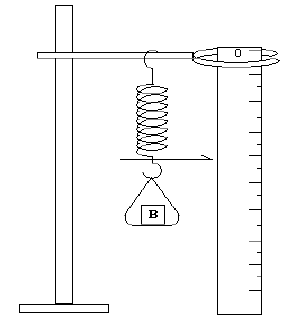
\includegraphics{./img/spring-practical.png}
\end{center}

\begin{itemize}
\item[]
\begin{itemize}
\item[(i)] Set up the apparatus as shown in the figure with zero mark of the metre-rule at the top of the rule and record the scale reading by the pointer, $S_0$.
\item[(ii)] Place the object ``B'' and standard weight (mass) W equal to 20 g in the pan and record the new pointer reading $S_1$. Calculate the extension, $e = S_1 - S_0$ in cm.
\item[(iii)] Repeat the procedure in (ii) above with W = 40 g, 60 g, 80 g and 100 g.
\end{itemize}
\item[(a)] Record your results in tabular form as shown below:\\
Table of Results:

\begin{tabular}{|p{2cm}|p{3cm}|p{3cm}|p{3cm}|}\cline{1-1}
\multicolumn{1}{|p{2cm}|}{$S_0 = $}&\multicolumn{2}{c}{} & \multicolumn{1}{p{2.5cm}}{} \\ \hline
\multicolumn{1}{|c|}{Mass} & \multicolumn{1}{c|}{Force, F (N)} & \multicolumn{1}{c|}{Pointer reading $S_1$} & \multicolumn{1}{c|}{Extension}\\
\multicolumn{1}{|c|}{(kg)} & \multicolumn{1}{c|}{} & \multicolumn{1}{c|}{(cm)} & \multicolumn{1}{c|}{$= S_1 - S_0$ (cm)}\\ \hline
\multicolumn{1}{|c|}{0} & \multicolumn{1}{c|}{} & \multicolumn{1}{c|}{} & \multicolumn{1}{c|}{}\\ 
\multicolumn{1}{|c|}{0.02} & \multicolumn{1}{c|}{} & \multicolumn{1}{c|}{} & \multicolumn{1}{c|}{}\\ 
\multicolumn{1}{|c|}{0.04} & \multicolumn{1}{c|}{} & \multicolumn{1}{c|}{} & \multicolumn{1}{c|}{}\\ 
\multicolumn{1}{|c|}{0.06} & \multicolumn{1}{c|}{} & \multicolumn{1}{c|}{} & \multicolumn{1}{c|}{}\\ 
\multicolumn{1}{|c|}{0.08} & \multicolumn{1}{c|}{} & \multicolumn{1}{c|}{} & \multicolumn{1}{c|}{}\\ 
\multicolumn{1}{|c|}{0.10} & \multicolumn{1}{c|}{} & \multicolumn{1}{c|}{} & \multicolumn{1}{c|}{}\\ \hline
\end{tabular}
\item[(b)] Plot graph of Force F (vertical axis) against extension $e$ (horizontal axis).
\item[(c)] Use your graph to evaluate
\begin{itemize}
\item[(i)] mass of B
\item[(ii)] spring constant, K, given that force, extension, constant and weight of B are related as follows:\\
F = K$e$ - B
\end{itemize}
\end{itemize}

%The aim of this experiment is to determine the mass of a given object $B$, and the
%constant of the spring provided.
%
%\begin{center}
%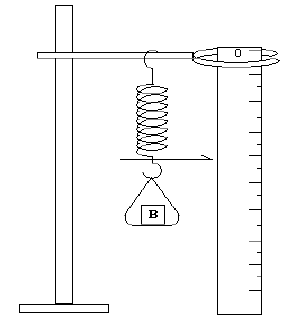
\includegraphics{./img/spring-practical.png}
%\end{center}
%
%\begin{enumerate}
%\item{Set up the apparatus as shown with the zero mark of the meter-rule at the top
%of the rule and record the scale reading, as shown by the pointer, $S_0$.}
%\item{Place the object $B$ and standard weight (mass) $W$ equal to 20~g in the pan
%and record the new pointer reading, $S_1$. Calculate the extension, $e = S_1 - S_0$ in
%cm.}
%\item{Repeat the procedure above with $W$ = 40~g, 60~g, 80~g and 100~g.}
%\item{Record your results in tabular form as shown below:
%
%\begin{center}
%\begin{tabular}{ | c | c | c | c | c | }
%\hline
%$S_0$ & Mass (kg) & Force, $F$ (N) & Pointer Reading $S_1$ (cm) & Extension, $e = S_1 - S_0$ (cm) \\ \hline
%& 0 & & & \\ \hline
%& 0.02 & & & \\ \hline
%& 0.04 & & & \\ \hline
%& 0.06 & & & \\ \hline
%& 0.08 & & & \\ \hline
%& 0.1 & & & \\ \hline
%\end{tabular}
%\end{center}
%
%}%Record your results...
%\item{Plot a graph of force $F$ (vertical axis) against extension $e$ (horizontal axis).}
%\item{Use your graph to evaluate
%\begin{enumerate}
%\item{mass of $B$}
%\item{spring constant, $K$, given that the force, extension, constant and
%weight of $B$ are related as follows: $$F = Ke - B$$}
%\end{enumerate}
%}%Use your graph...
%\end{enumerate}

\subsubsection{Discussion}

This practical has two parts: the first is to find the spring constant $k$, the second is
to find the mass of an unknown object $B$. By looking at the equation above, we
can see that $F$ is the dependent variable, $e$ is the independent variable, $K$ is the slope and
$-B$ is the intercept. When the graph is drawn, $K$ and $B$ can be found easily. Note that the
intercept on the graph will be negative.

The procedure is simply to start from a certain point on the metre rule (it does not
need to be a specific number) and to add masses one at a time, measuring the distance
from your starting point to the new position. This distance is called the extension, $e$. Be
sure that you are not simply reading the metre rule, but are measuring the distance from
the starting point.

\subsection{Simple Pendulum (Form 2)}

With some practice, this experiment should be simple for anyone to perform. The
trick comes with the math and graphing (again, an example is shown below). The
materials can all be local (string, stones, ruler) except for the stopwatches (for which you
should consult the materials section).

The practical usually has one objective: to find the acceleration due to gravity, $g$.
We know that the mass of a pendulum and its angle of deflection (for small angles) do
not affect its period. Therefore we vary only the length $L$ of the pendulum and measure
its period, as shown in the following example question.

\subsubsection{Sample Practical Question}

The aim of this experiment is to determine the magnitude of the acceleration due to
gravity, $g$. Proceed as follows:

\begin{center}
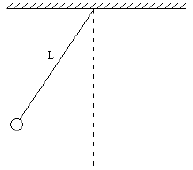
\includegraphics{./img/pendulum.png}
\end{center}


\begin{enumerate}
\item{Make a simple pendulum by suspending a weight on a string 10~cm long from a retort
stand.}
\item{Allow the pendulum to swing for twenty oscillations, using a stopwatch to record the
time. Repeat this procedure for pendulum lengths of 20~cm, 30~cm, 40~cm, and 50~cm.}
\item{Record your results in tabular form as shown below}

\begin{center}
\begin{tabular}{ | c | c | c | c | }
\hline
Pendulum Length l (m) & Time for 20 oscillations (s) & Period $T = \frac{t}{20}$ (s) & $T^2$ ($s^2$) \\ \hline
0.1 & & & \\ \hline
0.2 & & & \\ \hline
0.3 & & & \\ \hline
0.4 & & & \\ \hline
0.5 & & & \\ \hline
\end{tabular}
\end{center}

\item{Plot a graph of $T^2$ (vertical axis) against Pendulum Length (horizontal axis).}
\item{Calculate the slope of the graph.}
\item{Use the slope to calculate the value of $g$.}
\item{What are possible sources of error in this experiment?}

\end{enumerate}

\subsubsection{Discussion}

The period of a pendulum can be calculated using $$T = 2\pi\sqrt{\frac{l}{g}}$$
where $l$ is the length of the pendulum, $T$ is the period and $g$ is the acceleration due to
gravity. By squaring both sides, we get a much easier equation to graph: $$T^2 = 4\pi\frac{l}{g}$$ In this equation we see that $T^2$ is the dependent variable (y-axis) and $l$ is the
independent variable (x-axis), so the slope must be $$\mathrm{slope} = \frac{4\pi}{g}$$ 
When the graph is complete, the value of $g$ can be calculated easily.

Many students are confused by the difference between the time for many oscillations and
the period, which is the time for one oscillation. Be sure that they can change between
the two easily.

Note that pendulum practicals do not always require students to find $g$. Sometimes they are just required to find the relationship between $l$ and $t$. Again, it is essential that students read and understand the examination question, rather than memorize past solutions, and that they have lots of practice in collecting, organizing, and graphing data from a variety of experiments.

\subsection{Principle of Moments (Form 2)}

This experiment is used to verify the Principle of Moments, or equilibrium, by
balancing a meter rule on a knife-edge with masses at various distances. For this experiment, students need
a solid understanding of the Center of Gravity, the Moment of a force, and equilibrium.
Questions can range from finding the mass of an object to asking for
the mass of the metre rule. They are all
variations on the same practical: using the condition of equilibrium to find mass.

The following example is from the 2011 NECTA exam and asks students to find the mass of a battery using the Principle of Moments. Following is a brief explanation of the alternative practical of finding the mass of a metre rule.

\subsubsection{Finding the Mass of an Object}

\noindent \textbf{Sample Practical Question}\\

\noindent The aim of this experiment is to determine the mass of a given dry cell size ``AA''. Proceed as follows:
\begin{itemize}
\item[(a)] Locate and note the centre of gravity $C$ of the metre rule by balancing it on the knife edge.
\item[(b)] Suspend the 50 g mass at length `$a$' cm on one side of the metre rule and the 20 g mass together with the dry cell at length `$b$' cm on the other side of the metre rule. Fix the 50 g mass at length 30 cm from the fulcrum and adjust the position of the 20 g mass together with the dry cell until the metre rule balances horizontally. Read and record the values of $a$ and $b$ as $a_0$ and $b_0$ respectively.
\item[(c)] Draw the diagram for this experiment.
\item[(d)] By fixing $a = 5$ cm from fulcrum $C$, find its corresponding length $b$.
\item[(e)] Repeat the procedure in (d) above for $a = 10$ cm, 15 cm, 20 cm and 25 cm. Tabulate your results.
\item[(f)] Draw a graph of `$a$' against `$b$' and calculate its slope $G$.
\item[(g)] Calculate $X$ from the equation $50 = \cfrac{b_0}{a_0}(20 + X)$.
\item[(h)] Comment on the value of $\cfrac{b_0}{a_0}$.
\item[(i)] Sate the principle governing this experiment.
\end{itemize}

\noindent \textbf{Discussion}\\
This practical utilizes the Principle of Moments to find the mass of a ``AA'' battery. Initially, a known mass of 50 g is balanced with the (battery $+$ 20 g mass) system. Note that `$a$' and `$b$' are measured \emph{from the fulcrum} and so students should be careful not to just read the cm mark on the ruler where each object is suspended.

Also note that students are required to actually find the centre of gravity $C$ of the ruler rather than assuming it to be the 50 cm mark. This measured value of $C$ is to be used as the starting point for all future measurements of $a$ and $b$.

In part (g), students should recognize the equation $50 = \cfrac{b_0}{a_0}(20 + X)$ as coming from the Principle of Moments. Starting with
$$F_{\mathrm{clockwise}} \times d_{\mathrm{clockwise}} = F_{\mathrm{anticlockwise}} \times d_{\mathrm{anticlockwise}}$$
we get $$(mg)_{\mathrm{clockwise}} \times d_{\mathrm{clockwise}} = (mg)_{\mathrm{anticlockwise}} \times d_{\mathrm{anticlockwise}}$$
or $$(50 \text{g})(g) \times a_0 \text{ cm} = (20 \text{g} + X \text{g})(g) \times b_0 \text{ cm}$$
Canceling $g$ and dividing by $a_0$ reveals
$$50 = \cfrac{b_0}{a_0}(20 + X)$$
where $\cfrac{b_0}{a_0}$ is the ratio of the lever arm distances for the two weights being used. If the mass of the battery $X$ is less than 30 g, this ratio should be greater than 1, but if the mass is greater than 30 g, the ratio should be less than 1.

\subsubsection{Finding the Mass of a Metre Rule}

This question is less frequently seen on NECTA exams as compared to finding an unknown mass. However, it utilizes the same principles of equilibrium and balancing moments, and therefore is a useful alternative practical to ensure that students understand the concept rather than memorizing solutions to one version of the problem.

The mass of a uniform solid object, like a metre rule, is assumed to be at the
center of the object. In the case of the metre rule, we can say that the center of mass is at
the 50~cm mark, directly in the center. If we want it to be in equilibrium, the moments on
either side of a pivot must be equal, or $$ \mathrm{\text{Clockwise moment}} = \mathrm{\text{Anticlockwise moment}}$$
To find the mass of the metre rule itself, we begin by placing a known mass at one
point on the metre rule. We then move the pivot to one side or another until the metre
rule is perfectly balanced in equilibrium. As shown in the diagram below, the pivot will
not be at the 50~cm mark.

\begin{center}
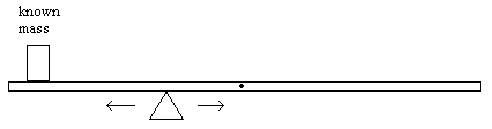
\includegraphics{./img/meter-rule.png}
\end{center}

If the metre rule is in equilibrium, we know that the moments must be equal, or
that $$F_{\mathrm{clockwise}} \times d_{\mathrm{clockwise}} = F_{\mathrm{anticlockwise}} \times d_{\mathrm{anticlockwise}}$$
In this case, the anticlockwise force is the weight of the object, and the distance is that
from the pivot to the object. The clockwise force is the weight of the metre rule, and the
distance is that from the 50~cm mark (center of mass) to the pivot. Therefore our
equation is: $$ W_{\mathrm{rule}} \times d_{\mathrm{rule}} = W_{\mathrm{object}} \times d_{\mathrm{object}} $$
Because the weight of the object is known, and the two distances can be measured, we
can easily calculate the mass and therefore the weight of the metre rule:
$$W_{\mathrm{rule}} = \frac{W_{\mathrm{object}} \times d_{\mathrm{object}}}{d_{\mathrm{rule}}}$$
From this we can calculate mass of the metre rule using $F = mg$.

%==============================================================================
\section{Light}
The light practical typically involves plane mirrors or glass blocks (rectangular
prisms). Presumably you will have already done these practicals with the students in Form
three (refraction) and Form 1 (plane mirrors), but a little practice will make the theory and
execution clear, especially if they can work in groups. The materials you will need are as
follows:
\begin{description}
\item[Cork Board]{Use cardboard for this, about 0.5 to 0.75~cm thick.}
\item[Optical pins]{Use sewing pins or syringe needles. If using syringe needs, be
sure to crimp the ends so students do not prick themselves.}
\item[Protractors]{These are cheap and students are supposed to have them anyway.
Small ones come in local mathematical sets.}
\item[Glass Block / Rectangular Prism]{A simple rectangular piece of 6~mm glass,
about 8~cm by 12~cm, will work.}
\item[Plane Mirror]{You can buy mirror glass in town in small sections for 200/= or
less; it should be available in villages through the local craftsmen if they work on
windows. Alternately, you can smoke one side of a piece of glass to make the
other side like a mirror.}
\end{description}

\subsection{Plane Mirror (Reflection) (Form 1)}

These are not as common as the rectangular prism, but they come in a variety of
questions:
\begin{itemize}
\item{Placing pins in front of a mirror at different distances and finding the distance of
the image.}
\item{Verifying the Law of Reflection at plane mirrors.}
\item{Placing two mirrors at different relative angles to find the number of images
produced.}
\end{itemize}
These are not overly complicated, but you should definitely practice with your students creating images in
mirrors -- they are not as accustomed to playing with mirrors as you might be.

Given below is an example practical from the 2006 NECTA exam which asks students to find a relationship between object distance and image distance in a plane mirror.

\subsubsection{Sample Practical Question}

Set up the experiment as shown in the diagram below using plane mirror, soft board, three pins and a white sheet of paper.

\begin{center}
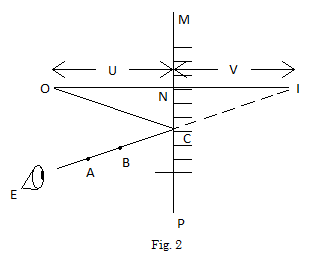
\includegraphics[width=8cm]{./img/2006-2-alt.png}
\end{center}

Fix a white sheet of paper on the soft board. Draw a line across the width at about the middle of the white sheep (MP). Draw line ONI perpendicular to MP.

Fix optical pin O to make ON = U = 3 cm. By using plasticine or otherwise, fix plane mirror along portion of MP with O in front of the mirror. With convenient position of eye, E, look into the mirror and fix optical pins A and B to be in line with image, I, of pin O.

Measure and record NI = V. Repeat procedure for U = 6 cm, 9 cm and 12 cm.

\begin{enumerate}
\item[]
\begin{enumerate}
\item[(a)] Tabulate your results as follows:

\quad \begin{tabular}{|c|c|c|c|c|} \hline
U (cm) & 3 & 6 & 9 & 12 \\ \hline
V (cm) & & & & \\ \hline
\end{tabular}

\item[(b)] Plot graph of U against V.
\item[(c)] Calculate slope, $m$ of the graph to the nearest whole number.
\item[(d)] State relationship between U and V.
\item[(e)] Write equation connecting U and V using numerical value of $m$ with symbols U and V.
\item[(f)] From your equation give position of the image when object is touching the face of the mirror.
\end{enumerate}
\end{enumerate}

\subsubsection{Discussion}
For a plane mirror, object distance and image distance are equal. That is, U and V should be approximately equal values for this practical. Note that students should extend line ONI far behind the mirror since they don't know where exactly the image I is going to be. The location of I is found at the intersection of the extended line ONI and the extended line AB connecting the two optical pins.

From the graph, the slope should be found to be 1 after rounding to the nearest whole number. From this, we can see that U = V. When the object is touching the face of the mirror, the object distance U is 0, and so the image distance V will also be 0.

\subsection{Rectangular Prism (Refraction) (Form 3)}

Students will be asked to find the refractive index and/or critical angle of the glass block by varying
the angle of incidence $i$ and measuring the corresponding angles of refraction $r$ as
described in the Mathematics section earlier. They will do this by placing two pins in
front of the prism, which together form a `ray' (the light ray), and then placing two more
pins on the other side of the prism so that, when observed through the prism from either
side, the four pins line up exactly. By drawing the lines that the pins make on the paper,
the refracted ray inside the prism can be easily traced, and the refracted angle measured.
An example question from the 2007 NECTA is given below.

\subsubsection{Sample Practical Question}

The aim of this experiment is to find the refractive index of a glass block. Proceed
as follows:\\

Place the given glass block in the middle of the drawing paper on the drawing
board. Draw lines along the upper and lower edges of the glass block. Remove the
glass block and extend the lines you have drawn. Represent the ends of these line
segments as $SS_1$ and $TT_1$. Draw the normal $NN_1$ to the parallel lines $SS_1$ and
$TT_1$ as shown in the figure below:

\begin{center}
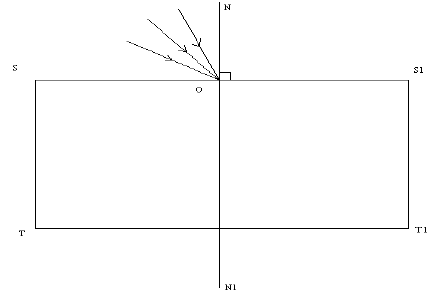
\includegraphics{./img/light-block-1.png}
\end{center}

Draw five evenly spaced lines from O to represent incident rays at different
angles of incidence (10$^\circ$, 20$^\circ$, 30$^\circ$, 40$^\circ$, and 50$^\circ$ from the normal). Replace the
glass block carefully between $SS_1$ and $TT_1$. Stick two pins $P_1$ and $P_2$ as shown in
the figure as far apart as possible along one of the lines drawn to represent an
incident ray. Locate an emergent ray by looking through the block and stick pins
$P_3$ and $P_4$ exactly in line with images $I_1$ and $I_2$ of pins $P_1$ and $P_2$. Draw the
emergent ray and repeat the procedure for all the incident rays you have drawn. Finally draw in the corresponding refracted rays.

\begin{center}
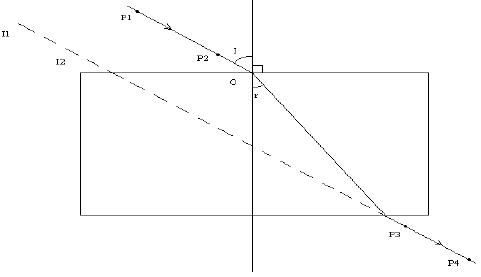
\includegraphics{./img/light-block-2.png}
\end{center}

\begin{enumerate}
\item[]
\begin{enumerate}
\item[(a)]{Record the angles of incidence $i$ and the measured corresponding angles of
refraction $r$ in a table. Your table of results should include the values of
$\sin{i}$ and $\sin{r}$.}
\item[(b)]{Plot the graph of $\sin{i}$ (vertical axis) against $\sin{r}$ (horizontal axis).}
\item[(c)]{Determine the slope of the graph.}
\item[(d)]{What is the refractive index of the glass block used?}
\item[(e)]{Mention any sources of errors in this experiment.}
\end{enumerate}
\end{enumerate}

\subsubsection{Discussion}

In this experiment, pins are used to simulate a ray of light. If all of the pins are
aligned as you look through the block, they act as a single ray. It takes practice to be able
to align the pins while looking through the block, so practice often with your students.

Light slows down as it enters a denser medium, so in order to minimize the time
required to pass through that medium, it changes direction until it moves back into its
original medium. In this case, light is moving from air into glass and then back into air,
so its direction changes while inside the glass, then returns to its original direction when
passing back into air. This effect is called refraction and it depends on the nature of the
media, in this case air and glass. Snell’s law gives us the relationship between the nature
of the media and the resulting angles of incidence and refraction:
$$n_1 \times \sin{i} = n_2 \times \sin{r}$$

In this experiment, the incident angle $i$ is being changed and the refracted angle $r$
is being measured. The refractive index of medium 1 (air) is known as 1.0, so we can use
these three to find the refractive index of medium 2 (glass). On the graph, $\sin{i}$ is the
dependent variable and $\sin{r}$ is the independent variable, so the equation becomes
$$\sin{i} = \sin{r} \frac{n_2}{n_1}$$
In this case the slope must be $\frac{n_2}{n_1}$.

The refractive index of medium air is simply 1.0, so the slope is the refractive index of
medium 2.

This practical is one of the easiest to perform with students because it does not
require much preparation. Syringe needles should be readily available and glass blocks are
cheap, so it is possible to have every students try this themselves many times before
taking the exam.

\subsubsection{Finding the Critical Angle}
Some questions may ask students to find the critical angle of a glass block in addition to its refractive index. The relationship between critical angle, $C$, and refractive index, $n$, for a particular medium is given by 
$$n = \frac{1}{\sin{C}}$$ or $$\frac{\sin{i}}{\sin{r}} = \frac{1}{\sin{C}}$$.

Thus a graph of $\sin{i}$ against $\sin{r}$ can be used to find the critical angle. However, take care to note that we must first take the reciprocal of the slope, i.e.
$$\sin{C} = \frac{1}{n}$$.

This gives us $\sin{C}$, so to get $C$ by itself, we need to use mathematical tables. Turn to the page for Natural Sines and search the table for the 4-figure value you obtained above by taking $\frac{1}{\text{slope}}$. The corresponding row gives the angle in degrees and the column gives the additional minutes of the angle.

For example, say we plot our graph of $\sin{i}$ ($y$-axis) against $\sin{r}$ ($x$-axis) and we calculate the slope to be 1.43. This is the refractive index of the glass block (since we can remember that glass has a refractive index of 1.5, we can do a quick mental check to make sure this makes sense). Then $\sin{C} = \frac{1}{1.43} = 0.6993$. From the mathematical tables, we get $C = 44^\circ 22'$ [6993 falls between 6984 ($18'$) and 6997 ($24'$), so we use the Mean Differences table to add on $4'$ giving a total of $22'$].

Note that the method of finding $n$ and $C$ changes if we are instead told to graph $\sin{r}$ ($y$-axis) against $\sin{i}$ ($x$-axis). Be sure to practice both versions with students to ensure their understanding.

%==============================================================================
\section{Electricity}

This is by far the least attempted practical on the exam, but not because it is
difficult. The electricity practical, if properly set up, is one of the easiest to perform. It
can appear in many different forms but will typically involve a simple circuit and some
kind of variable resistor in order to measure current or EMF for different resistances. The
materials you will probably need are as follows:

\begin{description}
\item[Connecting Wires]{Use speaker wire; it is cheap and available in most villages
and towns.}
\item[Voltmeters, Ammeters, Galvanometers]{This is unavoidable; you can get full
digital multimeters in town for about 10,000/=, galvanometers can be found in
any lab store or can be made using a compass and insulated copper wire.}
\item[Batteries]{Two to four D-size batteries should easily be enough for these experiments. Try to avoid Tiger brand if possible. Panasonic is highly superior in quality for roughly the same price.}
\item[Resistance Wire]{These are used to make small resistors for
the metre bridge or potentiometer. The most common type of wire to use is
nichrome, which can be found in a hardware or lab store. Steel will also work, though it
is less resistant and therefore harder to measure.}
\item[Metre Bridges]{See the activity that describes the construction of a metre bridge
and potentiometer. It is best to make both together as the construction is almost
identical and both are used frequently.}
\item[Variable Resistor (Rheostat)]{This is optional as it is typically only used to set a
level that can be easily read by the voltmeter. However, if you are using a
multimeter, you can simply change the magnitude setting on the multimeter to
account for unusually low or high resistances.}
%See How to Use a Rheostat
\item[Soldering Iron]{Not required, but may be a good investment for making reliable battery connections. Using electrical tape can lead to inconsistencies. Check large towns, prices should range from 10,000/= to 20,000/=.}
\end{description}

\subsection{Potentiometers (Form 3)}

This experiment is very simple but requires the correct materials, namely the
meter bridge/potentiometer described above. A complete circuit is created with a switch
(optional), power source, variable resistor and 1~m of bare resistance wire, all in series.

The potentiometer itself is simple to construct; all preparation is done by the teacher, so
the student simply follows the instructions as shown in the following example from the 2007 NECTA.

\subsubsection{Sample Practical Question}

The aim of this experiment is to determine the potential fall along a uniform
resistance wire carrying a steady current. Proceed as follows:

\begin{center}
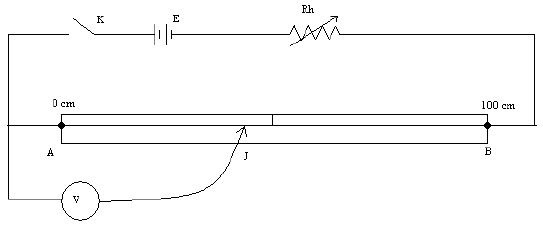
\includegraphics[width=10cm]{./img/meter-bridge-1.png}
\end{center}


Connect up the circuit as shown in the figure. Adjust the rheostat so that when the sliding
contact J is near B and the key is closed the voltmeter V indicates an almost full scale
of deflection. Do not alter the rheostat again.

Close key K and make contact with J, so that AJ = 10~cm. Record the potential
difference V volts between A and J as registered on the voltmeter.

Repeat this procedure for AJ = 20~cm, 30~cm, 50~cm, and 70~cm.

\begin{enumerate}
\item[]
\begin{enumerate}
\item[(a)]{Tabulate your results for the values of AJ and V.}
\item[(b)]{Plot a graph of V (vertical axis) against AJ (horizontal axis).}
\item[(c)]{Calculate the slope of the graph.}
\item[(d)]{What is your comment on the slope?}
\item[(e)]{State any precautions on the experiment.}
\end{enumerate}
\end{enumerate}

\subsubsection{Discussion}

This is a simple test of the relationship between the length of a wire and its
resistance, which we know is $$R=\frac{\rho l}{A} $$

Where $l$ is the length of the wire, $\rho$ is the resistivity of the wire, and $A$ is the cross-sectional
area of the wire. We expect that as the length of wire increases, its potential difference
will also increase. This is because the resistance (and therefore potential difference) of a wire is
directly related to its length. The voltmeter in this experiment is measuring just the
potential difference over the length of wire (10~cm, 20~cm, etc.), so if we use Ohm’s Law to say that $V = IR$, we can write:\\
$$ V = \frac{I \rho l}{A} $$
In this experiment, $I$, $\rho$ and $A$ are all constant, so the slope is
$$\mathrm{slope} = \frac{I \rho}{A} $$
Though it is not asked for directly in the question, we can find the resistivity, $\rho$, by measuring $I$ with an ammeter/galvanometer and $A$ with vernier calipers or a micrometer screw gauge.

\subsection{Metre Bridges (Form 3)}

A metre bridge resembles a potentiometer, except that it uses a galvanometer to
measure the difference in current between two points on the circuit, hence the name
``bridge.'' The same materials can be used as with the potentiometer, though it is best to
use small coils of resistance wire for the small resistors (between 3$\Omega$ and 20$\Omega$ is a good resistance). A galvanometer can be made easily if one is not available.

\begin{center}
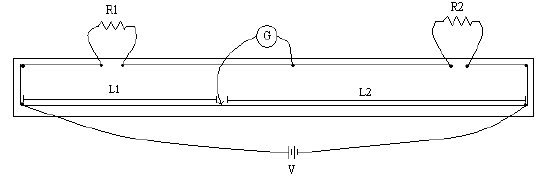
\includegraphics[width=10cm]{./img/meter-bridge-2.png}
\end{center}

Resistors $R_1$ and $R_2$ have different resistances, but they should be somehow similar so
that one resistor does not take all of the current (this will make it difficult to measure the
length to the galvanometer). About 5$\Omega$ and 10$\Omega$, for example, would work well.

However, for the sake of the practical, one resistor should not be known; the objective of
the practical is to find the unknown resistance. The long wire along the bottom edge is a
metre of nichrome wire or other resistance wire. One terminal of the galvanometer is
connected between the two resistors, and the other terminal is connected to a flying wire (or jockey)
that is free to move along the length of the nichrome wire.

The practical instructs you to move the galvanometer's flying wire back and forth
along the nichrome wire until it reads zero. At this point, we know that no current is
passing through the galvanometer, so the potential difference across it is zero. This
means that the current flowing through $R_1$ is the same as that current flowing through $R_2$,
and the current flowing through the nichrome wire is constant. From this we can
conclude that
$$ \frac{R_1}{L_1} = \frac{R_2}{L_2} $$
or that the ratio of the two resistors is equal to the ratio of distances from the flying wire
to either end of the nichrome wire. The resistance of one resistor (say, $R_1$) is known and
the lengths $L_1$ and $L_2$ can be measured from the flying wire to either side of the
nichrome wire. Using the ratio above, we can easily calculate the unknown resistance $R_2$.

An example is given below from the 2006 NECTA exam.

\subsubsection{Sample Practical Question}
You are required to determine the unknown resistance labeled X using a metre bridge circuit. Connect your circuit as shown below, where $R$ is a resistance box, G is a galvanometer, J is a jockey and others are common circuit components.

\begin{center}
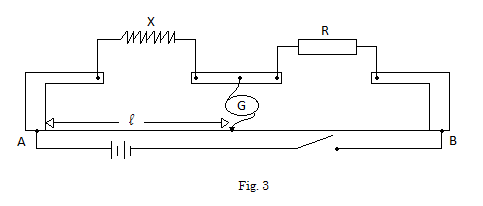
\includegraphics[width=12cm]{./img/2006-3-alt.png}
\end{center}

Procedure:\\

With $R$ = 1 $\Omega$, obtain a balance point on a metre bridge wire AB using a jockey J. Note the length $l$ in centimetres. Repeat the experiment with R equal to 2 $\Omega$, 4 $\Omega$, 7 $\Omega$ and 10 $\Omega$.\\

Tabulate your results for $R$, $l$ and $^1/_l$.

\begin{itemize}
\item[(a)]
\begin{itemize}
\item[(i)] Plot a graph of $R$ (vertical axis) against $^1/_l$ (horizontal axis).
\item[(ii)] Determine the slope S of your graph.
\item[(iii)] Using your graph, find the value of $R$ for which $^1/_l = 0.02$.
\end{itemize}
\item[(b)] Read and record the intercept $R_0$ on the vertical axis.
\item[(c)] Given that,\\
\quad \quad $R = \cfrac{100 \text{X}}{l} - \text{X}$\\
Use the equation and your graph to determine the value of X.
\item[(d)] Comment on your results in (a)(iii), (b) and (c) above.
\end{itemize}

\subsubsection{Discussion}
The procedure for this question is similar to most other wheatstone bridge problems: vary a known resistor and see how it affects the relative lengths in resistance wire required to balance the potential difference and give no current through the galvanometer. It may not be obvious at first, however, where the equation $R = \frac{100 \text{X}}{l}$ - X comes from.

Starting with the balancing ratio for a wheatstone bridge, $$ \frac{R_1}{L_1} = \frac{R_2}{L_2} $$ we can solve for the unknown resistor $$R_2 = R_1\left(\frac{L_2}{L_1}\right)$$. 

Recall that $L_1$ and $L_2$ are the corresponding lengths from either end of the metre rule to the jockey (in cm), and so taking them together, we get $$L_1 + L_2 = 100$$. Dividing both sides by $L_1$ gives $$1 + \frac{L_2}{L_1} = \frac{100}{L_1}$$. Then solving for $\frac{L_2}{L_1}$, $$\frac{L_2}{L_1} = \frac{100}{L_1} - 1$$. Now substitute this into our previous equation for $R_2$: $$R_2 = R_1\left(\frac{100}{L_1} - 1\right)$$. Replacing $R_2$ with $R$, $L_1$ with $l$ and $R_1$ with X for this problem and distributing gives, $$R = \frac{100 \text{X}}{l} - \text{X}$$.

From this equation, we have dependent variable $R$, independent variable $\frac{1}{l}$, slope $100 \text{X}$ and $y$-intercept $-\text{X}$. So we can obtain the value of the unknown resistor X either by using the $y$-intercept (note the resistance is a positive value) or by taking the slope divided by 100.

\subsection{Ohm’s Law (Form 2)}

The practical may give any kind of experiment to use or verify Ohm’s Law in a
simple circuit. Finding the e.m.f. and internal resistance of cells appears frequently. Students should be very familiar with the law, as well as the factors that determine resistance in a wire and the effect of internal resistance of a cell on a circuit. Given below is an example problem taken from the 2011 NECTA exam.

\subsubsection{Sample Practical Question}
You are provided with an ammeter, A, resistance box, R, dry cell, D, a key, K and connecting wires. Proceed as follows:
\begin{enumerate}
\item[]
\begin{enumerate}
\item[(a)] Connect the circuit in series.
\item[(b)] Put $R$ = 1 $\Omega$ and quickly read the value of current $I$ on the ammeter.
\item[(c)] Repeat procedure (b) above for $R$ = 2 $\Omega$, 3 $\Omega$, 4 $\Omega$ and 5 $\Omega$. Record your results in a tabular form.
\item[(d)] Draw the circuit diagram for this experiment.
\item[(e)] Plot the graph of $R$ against $\cfrac{1}{I}$.
\item[(f)] Determine the slope of the graph.
\item[(g)] If the graph obeys the equation $R=\cfrac{E}{I}-r$, then
\begin{enumerate}
\item[(i)] suggest how $E$ and $r$ may be evaluated from your graph.
\item[(ii)] compute $E$.
\item[(iii)] compute $r$.
\end{enumerate}
\item[(h)] State one source of error and suggest one way of minimizing it.
\item[(i)] Suggest the aim of this experiment.
\end{enumerate}
\end{enumerate}

\subsubsection{Discussion}
To see where the equation $R=\cfrac{E}{I}-r$ comes from, first start with Ohm's Law, $V = IR$. Accounting for the internal resistance of the cell, $r$, this becomes $$V = I(R + r)$$. To solve for resistance, we divide both sides by $I$, which gives $$(R + r) = \frac{V}{I}$$. From this we can see that, using $E$ as e.m.f. for this problem, $$R=\cfrac{E}{I}-r $$. 

In this form, the equation resembles the classic $y = mx + c$, where $R$ is the dependent variable, $\frac{1}{I}$ the independent variable, $E$ is the slope and $-r$ is the y-intercept (note the internal resistance is a positive value).

%\pagebreak
%
%\section{NECTA Past Papers}
%\setcounter{secnumdepth}{1}
%\subsection{2011 - PHYSICS 2A ACTUAL PRACTICAL A}

\begin{enumerate}
\item The aim of this experiment is to determine the mass of a given dry cell size ``AA''. Proceed as follows:
\begin{itemize}
\item[(a)] Locate and note the centre of gravity $C$ of the metre rule by balancing it on the knife edge.
\item[(b)] Suspend the 50 g mass at length `$a$' cm on one side of the metre rule and the 20 g mass together with the dry cell at length `$b$' cm on the other side of the metre rule. Fix the 50 g mass at length 30 cm from the fulcrum and adjust the position of the 20 g mass together with the dry cell until the metre rule balances horizontally. Read and record the values of $a$ and $b$ as $a_0$ and $b_0$ respectively.
\item[(c)] Draw the diagram for this experiment.
\item[(d)] By fixing $a = 5$ cm from fulcrum $C$, find its corresponding length $b$.
\item[(e)] Repeat the procedure in (d) above for $a = 10$ cm, 15 cm, 20 cm and 25 cm. Tabulate your results.
\item[(f)] Draw a graph of `$a$' against `$b$' and calculate its slope $G$.
\item[(g)] Calculate $X$ from the equation $50 = \cfrac{b_0}{a_0}(20 + X)$.
\item[(h)] Comment on the value of $\cfrac{b_0}{a_0}$.
\item[(i)] Sate the principle governing this experiment.
\end{itemize}
\end{enumerate}

\flushright \textbf{(25 marks)}
\begin{enumerate}
\item[2.] You are provided with an ammeter, A, resistance box, R, dry cell, D, a key, K and connecting wires. Proceed as follows:
\begin{enumerate}
\item[(a)] Connect the circuit in series.
\item[(b)] Put $R$ = 1 $\Omega$ and quickly read the value of current $I$ on the ammeter.
\item[(c)] Repeat procedure (b) above for $R$ = 2 $\Omega$, 3 $\Omega$, 4 $\Omega$ and 5 $\Omega$. Record your results in a tabular form.
\item[(d)] Draw the circuit diagram for this experiment.
\item[(e)] Plot the graph of $R$ against $\cfrac{1}{I}$.
\item[(f)] Determine the slope of the graph.
\item[(g)] If the graph obeys the equation $R=\cfrac{E}{I}-r$, then
\begin{enumerate}
\item[(i)] suggest how $E$ and $r$ may be evaluated from your graph.
\item[(ii)] compute $E$.
\item[(iii)] compute $r$.
\end{enumerate}
\item[(h)] State one source of error and suggest one way of minimizing it.
\item[(i)] Suggest the aim of this experiment.
\end{enumerate}

\end{enumerate}

\flushright \textbf{(25 marks)}
\flushleft
%\pagebreak
%\section{2010 - PHYSICS 2A ALTERNATIVE A PRACTICAL}

\begin{enumerate}
\item[1.] The aim of this experiment is to find the mass of the unknown load labeled ``$W$'' and the spring constant $K$. Proceed as follows:

\begin{center}
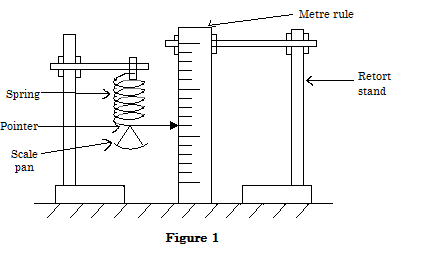
\includegraphics[width=14cm]{./img/2010-1-alt.png}
\end{center}

Set up the apparatus as shown in Figure 1. Put a mass of 50 g on the scale pan and record the equilibrium position $X_0$ of the pointer. Put on the scale pan the unknown weight marked $W$. Without removing $W$ and the 50 g mass in the scale pan, add a load $L$ of 50 g and record the new position of the pointer $X$. Calculate the extension $E = (X - X_0)$. Repeat this process for $L$ = 100 g, 150 g, 200 g and 250 g.
\begin{enumerate}
\item[(a)] Record you conclusions as shown in Table 1.\\[10pt]

Equilibrium position $X_0$..................\\[10pt]

Table 1\\[10pt]

%\begin{center}
\begin{tabular}{|p{3cm}|p{3cm}|p{3cm}|} \hline
\multicolumn{1}{|c|}{Load (g)} & \multicolumn{1}{c|}{$X$ (cm)} & \multicolumn{1}{c|}{$E = X - X_0$ (cm)} \\ \hline
\multicolumn{1}{|c|}{50} & & \\ \hline
\multicolumn{1}{|c|}{100} & & \\ \hline
\multicolumn{1}{|c|}{150} & & \\ \hline
\multicolumn{1}{|c|}{200} & & \\ \hline
\multicolumn{1}{|c|}{250} & & \\ \hline
\end{tabular}\\[10pt]
%\end{center}

\item[(b)] Plot the graph of load L against absolute value of extension E. The scale of the vertical axis should be chosen to range from 200 g to 300 g.
\item[(c)] From the graph, determine the unknown weight marked W, given that L = KE + W where K is a constant.
\item[(d)] What does the gradient of the graph represent?
\item[(e)] State the sources of errors and precautions that should be taken in the experiment.
\end{enumerate}
\end{enumerate}
\flushright \textbf{(25 marks)}

\pagebreak

\begin{enumerate}
\item[2.] The aim of this experiment is to determine the refractive index of water. Proceed as follows:

\begin{center}
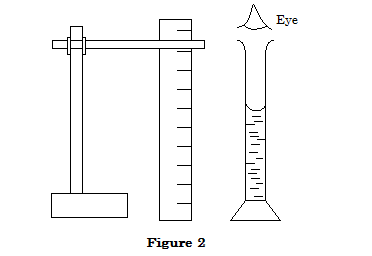
\includegraphics[width=10cm]{./img/2010-2-alt.png}
\end{center}

\begin{enumerate}
\item[(a)] Arrange your apparatus as in Figure 2. Put about 150 cm$^3$ of clear water in the measuring cylinder. Drop an office pin at the bottom so that it rests touching the wall of the cylinder.
\item[(b)] Look in the cylinder from Figure 2. Use another office pin as a search pin, move it up and down outside the cylinder, and locate the image position by no parallax method. Locate the image position of the ruler. Measure and record the depth ($H_1$) of the image. Measure and record the depth ($H_2$) of water. Repeat the experiment with 175 cm$^3$, 200 cm$^3$, 225 cm$^3$ and 250 cm$^3$ of water in the measuring cylinder.
\item[(c)] 
\begin{enumerate}
\item[(i)] Record in Table 2 your values of $H_1$ and $H_2$ corresponding to the volumes of water in the measuring cylinder.\\[10pt]

Table 2\\[10pt]

%\begin{center}
\begin{tabular}{|p{3cm}|p{3cm}|p{3cm}|} \hline
\multicolumn{1}{|c|}{Volume of water V (cm)} & \multicolumn{1}{c|}{$H_1$} & \multicolumn{1}{c|}{$H_2$} \\ \hline
\multicolumn{1}{|c|}{150} & & \\ \hline
\multicolumn{1}{|c|}{175} & & \\ \hline
\multicolumn{1}{|c|}{200} & & \\ \hline
\multicolumn{1}{|c|}{225} & & \\ \hline
\multicolumn{1}{|c|}{250} & & \\ \hline
\end{tabular}\\[10pt]
%\end{center}

\item[(ii)] Plot the graph of $H_2$ versus $H_1$.
\item[(iii)] Determine the slope of the graph.
\item[(iv)] What is the physical meaning of the slope?
\item[(v)] State sources of error in this experiment.
\end{enumerate}
\end{enumerate}
\end{enumerate}
\flushright \textbf{(25 marks)}

\pagebreak

\begin{enumerate}
\item[3.] The aim of this experiment is to determine the resistivity of an electrical conductor $P$.

\begin{center}
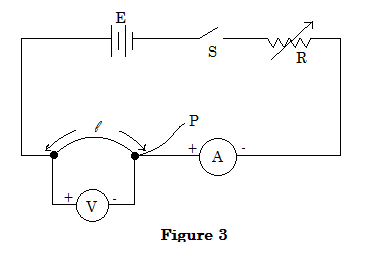
\includegraphics[width=10cm]{./img/2010-3-alt.png}
\end{center}

With $P$ having a length $l = 50$ cm, connect up the circuit as shown in Figure 3. Close one key S and adjust the rheostat R so that the current in $P$ is 0.20 A. Record the current $I$ and the potential difference $V$ between its ends.\\[10pt]

Repeat the procedure with current $I = $0.30 A, 0.40 A, 0.50 A and 0.60 A.
\begin{enumerate}
\item[(a)] Record your results in Table 3.\\[10pt]

Table 3\\[10pt]

%\begin{center}
\begin{tabular}{|p{3cm}|p{3cm}|} \hline
\multicolumn{1}{|c|}{Current $I$ (A)} & \multicolumn{1}{c|}{P.d. (volts)} \\ \hline
\multicolumn{1}{|c|}{0.20} &  \\ \hline
\multicolumn{1}{|c|}{0.30} &  \\ \hline
\multicolumn{1}{|c|}{0.40} &  \\ \hline
\multicolumn{1}{|c|}{0.50} &  \\ \hline
\multicolumn{1}{|c|}{0.60} &  \\ \hline
\end{tabular}\\[10pt]
%\end{center}

\item[(b)] Plot a graph of $V$ against $I$ and calculate the slope $G$.
\item[(c)] Deduce the resistivity of the conductor $P$ given that; $\rho = \cfrac{G\pi d^2}{4l}$.\\[10pt]
Where $\rho$ = resistivity\\
$d$ = diameter of $P$ (measured using the micrometer screw gauge provided).
\end{enumerate}
\end{enumerate}

\flushright \textbf{(25 marks)}
\flushleft
%\pagebreak
%\subsection{2009 - PHYSICS 2A ALTERNATIVE A PRACTICAL}

\begin{enumerate}
\item[1.] In this experiment you are required to find the relationship between the length of a simple pendulum and its period. Proceed as follows:
\begin{itemize}
\item[(a)] Suspend a simple pendulum of length L = 100 cm. Displace the pendulum through a small angle so that it swings parallel to the edge of the bench or table, determine the time for 20 oscillations. Continue reducing the length of the pendulum by 10 cm each time and obtain a total of six readings.
\item[(b)] Record your readings in a table as shown below.


\begin{tabular}{|p{2.5cm}|p{2.5cm}|p{2.5cm}|p{2.5cm}|p{2.5cm}|} \hline
Length of pendulum L (cm) & Log$_{10}$L & Time for 20 oscillations & Period T & Log$_{10}$T \\ \hline
&&&& \\ 
&&&& \\ 
&&&& \\ 
&&&& \\ 
&&&& \\ 
&&&& \\ 
&&&& \\ 
&&&& \\ \hline
\end{tabular}\\[10pt]

\noindent Assuming that T $ \propto $ L$^a$, we have T = $k$L$^a$ and taking logarithms to base ten on both sides we get $\log_{10}$T = $a\log_{10}$L + $\log_{10}k$.

\begin{itemize}
\item[(i)] Plot a graph of $\log_{10}$T (vertical axis) against $\log_{10}$L (horizontal axis) hence determine the values of $a$ and $k$ each correct to one decimal place.
\item[(ii)] From your answer in (i) above write down the values of $a$ and $k$ each in the form of $\cfrac{b}{c}$ where $b$ and $c$ are integers (i.e. whole numbers).
\item[(iii)] From the assumption and your answer in (ii) deduce the form of the equation governing the motion of the simple pendulum.
\end{itemize}

\end{itemize}
\end{enumerate}
\flushright \textbf{(25 marks)}


\begin{enumerate}
\item[2.] The aim of this experiment is to determine the refractive index $\eta$ of a given glass block.

\begin{center}
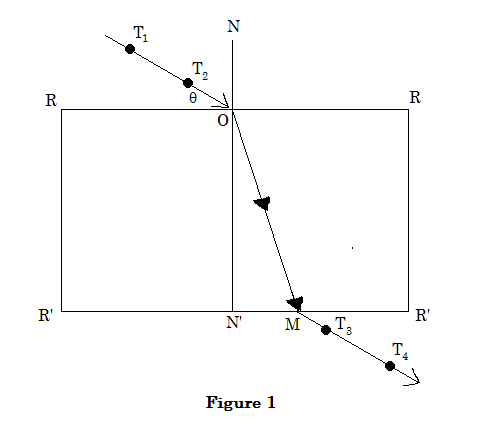
\includegraphics[width=8cm]{./img/2009-2-alt.png}
\end{center}

Place the rectangular glass block on the white paper on a drawing board. Using a pencil trace the outline of the block. Remove the glass block and draw a normal NOM near the left end of the block (Figure 1).\\[10pt]

\noindent Using a protractor and a pencil measure $\theta = 20^\circ$, draw a line making the angle $20^\circ$ with the surface RR of the block. Erect two pins T$_1$ and T$_2$ on this line and at a suitable distance from one another. Return the block and erect the pins T$_3$ and T$_4$ at positions such that they lie in a straight line with pins T$_1$ and T$_2$ as seen through the block. Now remove the block and draw a complete path of the ray (Figure 1).\\[10pt]

\noindent Measure the length MN$'$ and ON$'$: Repeat the procedure for values of $\theta = 30^\circ, 40^\circ$ and $60^\circ$ respectively. In each case make a drawing on a fresh part of the drawing paper.

\begin{itemize}
\item[(a)] Record the values of $\theta$, MN$'$, ON$'$, $\cfrac{\text{MN}'}{\text{ON}'}$ and $\cos \theta$ in a tabular form.
\item[(b)] Plot a graph of $\cfrac{\text{MN}'}{\text{ON}'}$ against $\cos \theta$.
\item[(c)] Find the slope $G$ of the graph.
\item[(d)] Calculate the value of the refractive index $\eta$; given that $G = \cfrac{1}{\eta}$.
\item[(e)] State two sources of errors. \hfill \textbf{(25 marks)}
\end{itemize}

\end{enumerate}


\begin{enumerate}
\item[3.] The aim of this experiment is to verify Ohm's Law.

\begin{center}
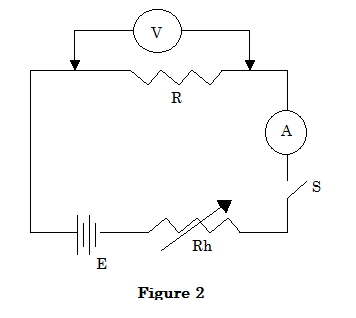
\includegraphics[width=7cm]{./img/2009-3-alt.png}
\end{center}

\begin{itemize}
\item[(a)] Set up the apparatus as shown on Figure 2, close switch S. Adjust the Rheostat Rh by sliding slowly from one end, read and record the value V of the voltmeter and current I of the ammeter.
\item[(b)] Repeat the experiment by changing the Rheostat slider to obtain about five pair of readings.\\[10pt]

\textbf{NB:} Adjust the Rheostat until when the pointer is exactly on the division of the metre scale.\\[10pt]

Table of results\\[10pt]
\begin{tabular}{|c|c|c|c|c|c|c|c|}\hline
V (V)&&&&&&&\\ \hline
I (A)&&&&&&& \\ \hline
\end{tabular}

\item[(c)] Plot a graph of V (vertical axis) against I (horizontal axis).
\item[(d)] 
\begin{itemize}
\item[(i)] Find the slope of the graph.
\item[(ii)] What is the relation between V and I?
\item[(iii)] Find the resistance R. \hfill \textbf{(25 marks)}
\end{itemize}
\end{itemize}

\end{enumerate}
\flushleft

%\pagebreak
%\section{2007 - PHYSICS 2A ALTERNATIVE A PRACTICAL}

\begin{enumerate}
\item[1.] The aim of this experiment is to determine the mass of a given object ``B'', and the constant of the spring provided.

\begin{center}
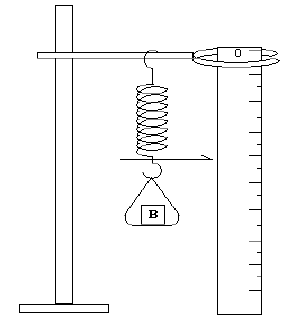
\includegraphics[width=7cm]{./img/2007-1-alt.png}
\end{center}

\begin{itemize}
\item[]
\begin{itemize}
\item[(i)] Set up the apparatus as shown in Fig. 1 with zero mark of the metre-rule at the top of the rule and record the scale reading by the pointer, $S_0$.
\item[(ii)] Place the object ``B'' and standard weight (mass) W equal to 20 g in the pan and record the new pointer reading $S_1$. Calculate the extension, $e = S_1 - S_0$ in cm.
\item[(iii)] Repeat the procedure in (ii) above with W = 40 g, 60 g, 80 g and 100 g.
\end{itemize}
\item[(a)] Record your results in tabular form as shown below:\\
Table of Results:

\begin{tabular}{|p{2cm}|p{3cm}|p{3cm}|p{3cm}|}\cline{1-1}
\multicolumn{1}{|p{2cm}|}{$S_0 = $}&\multicolumn{2}{c}{} & \multicolumn{1}{p{2.5cm}}{} \\ \hline
\multicolumn{1}{|c|}{Mass} & \multicolumn{1}{c|}{Force, F (N)} & \multicolumn{1}{c|}{Pointer reading $S_1$} & \multicolumn{1}{c|}{Extension}\\
\multicolumn{1}{|c|}{(kg)} & \multicolumn{1}{c|}{} & \multicolumn{1}{c|}{(cm)} & \multicolumn{1}{c|}{$= S_1 - S_0$ (cm)}\\ \hline
\multicolumn{1}{|c|}{0} & \multicolumn{1}{c|}{} & \multicolumn{1}{c|}{} & \multicolumn{1}{c|}{}\\ 
\multicolumn{1}{|c|}{0.02} & \multicolumn{1}{c|}{} & \multicolumn{1}{c|}{} & \multicolumn{1}{c|}{}\\ 
\multicolumn{1}{|c|}{0.04} & \multicolumn{1}{c|}{} & \multicolumn{1}{c|}{} & \multicolumn{1}{c|}{}\\ 
\multicolumn{1}{|c|}{0.06} & \multicolumn{1}{c|}{} & \multicolumn{1}{c|}{} & \multicolumn{1}{c|}{}\\ 
\multicolumn{1}{|c|}{0.08} & \multicolumn{1}{c|}{} & \multicolumn{1}{c|}{} & \multicolumn{1}{c|}{}\\ 
\multicolumn{1}{|c|}{0.10} & \multicolumn{1}{c|}{} & \multicolumn{1}{c|}{} & \multicolumn{1}{c|}{}\\ \hline
\end{tabular}
\item[(b)] Plot graph of Force F (vertical axis) against extension $e$ (horizontal axis).
\item[(c)] Use your graph to evaluate
\begin{itemize}
\item[(i)] mass of B
\item[(ii)] spring constant, K, given that force, extension, constant and weight of B are related as follows:\\
F = K$e$ - B
\end{itemize}
\end{itemize}

\end{enumerate}
\flushright \textbf{(25 marks)}



\begin{enumerate}
\item[2.] The aim of this experiment is to find the refractive index of a glass block. Proceed as following:\\[10pt]

Place the given glass block in the middle of the drawing paper on the drawing board. Draw lines along the upper and lower edge of the glass block. Remove the glass block and extend the line you have drawn. Represent the ends of those line segments as SS$^1$ and TT$^1$. Draw the normal NN$^1$ to the parallel lines SS$^1$ and TT$^1$ as shown in Fig. 2(a).

\begin{center}
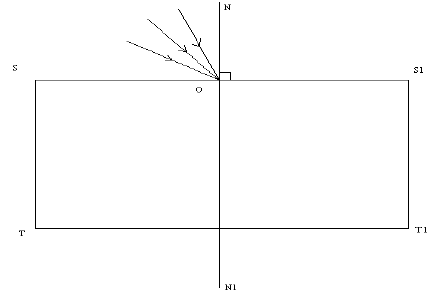
\includegraphics[width=8cm]{./img/2007-2a-alt.png}
\end{center}

Draw five evenly spaced lines from O to represent incident rays at different angles of incidence (10$^\circ$, 20$^\circ$, 30$^\circ$, 40$^\circ$ and 50$^\circ$ from the normal). Replace the glass block carefully between SS$^1$ and TT$^1$. Stick two pins P$_1$ and P$_2$ as shown in Fig. 2(b) as far apart as possible along one of the lines drawn to represent an incident ray. Locate an emergent ray by looking through the block and stick pins P$_3$ and P$_4$ exactly in line with images I$_1$ and I$_2$ of pins P$_1$ and P$_2$. Draw the emergent ray and repeat the procedure for all the incident rays you have drawn. Finally draw in the corresponding refracted rays.\\[10pt]

NOTE: The drawing paper should be handed in together with other answer sheets.

\begin{center}
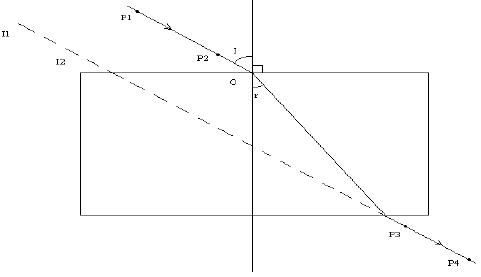
\includegraphics[width=10cm]{./img/2007-2b-alt.png}
\end{center}

\begin{itemize}
\item[(a)] Record the angles of incidence I and the measured corresponding angles of refraction ``r'' in a table. Your table of results should include the values of $\sin$ I and $\sin$ r.
\item[(b)] Plot the graph of $\sin$ I (vertical - axis) against $\sin$ r (horizontal - axis).
\item[(c)] Determine the slope of the graph.
\item[(d)] What is the refractive index of the glass block used?
\item[(e)] Mention any sources of errors in this experiment.
\end{itemize}

\end{enumerate}
\flushright \textbf{(25 marks)}


\begin{enumerate}
\item[3.] The aim of this experiment is to determine the potential fall along a uniform resistance wire carrying a steady current.\\[10pt]

Proceed as follows:

\begin{center}
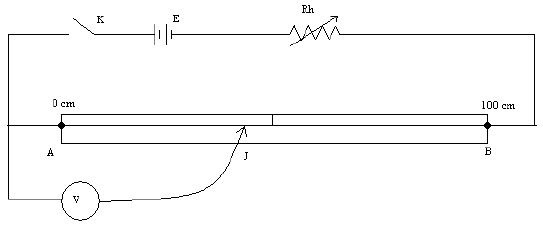
\includegraphics[width=12cm]{./img/2007-3-alt.png}
\end{center}

Connect up the circuit as shown in Fig. 3. Adjust the rheostat so that when the sliding contact J is near B, and the key is closed the voltmeter V indicates an almost full scale deflection. Do not alter the rheostat again.\\

Close key K and make contact with J, so that AJ = 10 cm. Record the potential different V volts between A and J as registered on the voltmeter.\\

Repeat this procedure for AJ = 20 cm, 30 cm, 50 cm and 70 cm.

\begin{itemize}
\item[(a)] Tabulate your results for the values of AJ and V.
\item[(b)] Plot a graph of V (vertical axis) against AJ (horizontal axis).
\item[(c)] Calculate the slope of the graph.
\item[(d)] What is your comment on the slope?
\item[(e)] State any precautions on the experiment.
\end{itemize}

\end{enumerate}
\flushright \textbf{(25 marks)}
\flushleft
%\pagebreak
%\section{2006 - PHYSICS 2A ALTERNATIVE A PRACTICAL}

\begin{enumerate}
\item[1.] In this experiment you are required to determine the mass of unknown object ``X''.

\begin{center}
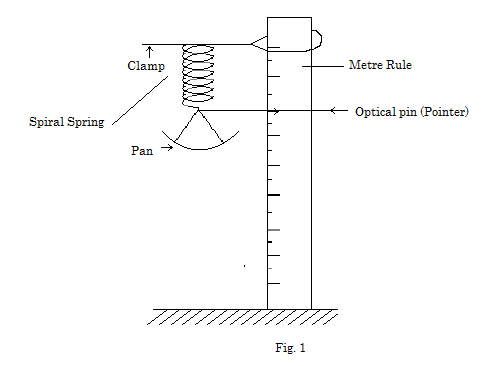
\includegraphics[width=10cm]{./img/2006-1-alt.png}
\end{center}

Assemble the pieces of apparatus as shown in Figure 1, with zero mark scale of the rule at the lower most end.\\

Record the reading of the position of pointer on the scale of metre-rule when the pan is empty as $S_0$.\\

Put 20 g to the pan and record pointer reading $S$.\\

Find extension $e = S - S_0$ cm.\\

Repeat the procedure for mass of 40 g, 60 g, 80 g and 100 g. Put object X on the pan and record its pointer reading.

\begin{itemize}
\item[(a)] Summarize your results in a table as follows:\\[10pt]
\begin{center}
\begin{tabular}{|l|c|c|c|c|c|c|} \hline
Mass on pan (g) &20&40&60&80&100&X \\ \hline
Pointer reading (cm) &&&&&& \\ \hline
Extension, $e = S - S_0$ (cm) &&&&&& \\ \hline
\end{tabular} \\[10pt]
\end{center}
\item[(b)] Plot graph of mas against extension (m Vs. $e$).
\item[(c)] Find slope, P, of your graph.
\item[(d)] Find mass X.
\item[(e)] Find Q, given that Q = P $\times$ $e_\text{x}$, where $e_\text{x}$ is extension of X.
\item[(f)] Comment on Q and X.
\end{itemize}


\end{enumerate}

\begin{enumerate}
\item[2.] Set up the experiment as shown in the diagram below using plane mirror, soft board, three pins and a white sheet of paper.

\begin{center}
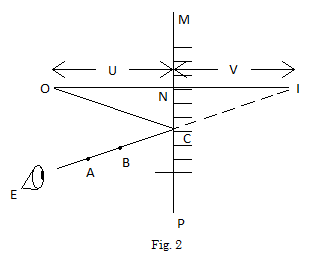
\includegraphics[width=6cm]{./img/2006-2-alt.png}
\end{center}

Fix a white sheet of paper on the soft board. Draw a line across the width at about the middle of the white sheep (MP). Draw line ONI perpendicular to MP.\\

Fix optical pin O to make ON = U = 3 cm. By using plasticine or otherwise, fix plane mirror along portion of MP with O in front of the mirror. With convenient position of eye, E, look into the mirror and fix optical pins A and B to be in line with image, I, of pin O.\\

Measure and record NI = V. Repeat procedure for U = 6 cm, 9 cm and 12 cm.

\begin{itemize}
\item[(a)] Tabulate your results as follows:\\[10pt]

\quad \quad \begin{tabular}{|l|c|c|c|c|} \hline
U (cm) &3&6&9&12 \\ \hline
V (cm) &&&& \\ \hline
\end{tabular} \\[10pt]

\item[(b)] Plot graph of U against V.
\item[(c)] Calculate slope, m, of the graph to the nearest whole number.
\item[(d)] State relationship between U and V.
\item[(e)] Write equation connecting U and V using numerical value of m with symbols U and V.
\item[(f)] From your equation give position of the image when object is touching the face of the mirror.
\end{itemize}

\end{enumerate}


\begin{enumerate}
\item[3.] You are required to determine the unknown resistance labeled X using a metre bridge circuit. Connect your circuit as shown below, where R is a resistance box, G is a galvanometer, J is a jockey and others are common circuit components.

\begin{center}
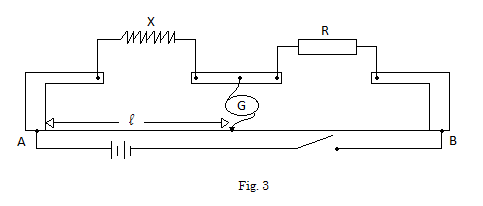
\includegraphics[width=14cm]{./img/2006-3-alt.png}
\end{center}

Procedure:\\

With R = 1 $\Omega$, obtain a balance point on a metre bridge wire AB using a jockey J. Note the length $l$ in centimetres. Repeat the experiment with R equal to 2 $\Omega$, 4 $\Omega$, 7 $\Omega$ and 10 $\Omega$.\\

Tabulate your results for R, $l$ and $^1/_l$.

\begin{itemize}
\item[(a)]
\begin{itemize}
\item[(i)] Plot a graph of R (vertical axis) against $^1/_l$ (horizontal axis).
\item[(ii)] Determine the slope S of your graph.
\item[(iii)] Using your graph, find the value of R for which $^1/_l = 0.02$.
\end{itemize}
\item[(b)] Read and record the intercept R$_0$ on the vertical axis.
\item[(c)] Given that,\\
\quad \quad R = $\cfrac{100\text{X}}{l}$ - X\\
Use the equation and your graph to determine the value of X.
\item[(d)] Comment on your results in (a)(iii), (b) and (c) above.
\end{itemize}

\end{enumerate}
%\pagebreak
%\subsection{2005 - PHYSICS 2A ALTERNATIVE A PRACTICAL}

\begin{enumerate}
\item[1.] The aim of this experiment is to determine the mass of unknown weight labelled \textbf{X} and the force constant of the spring \textbf{k}.

\begin{center}
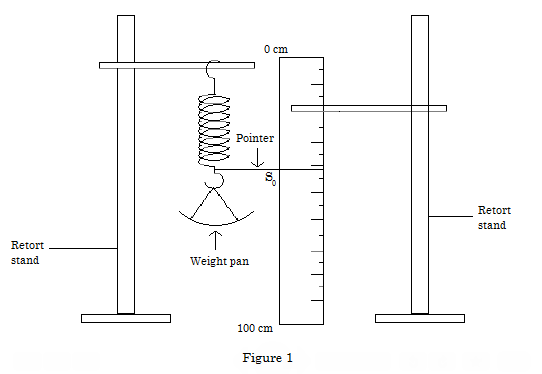
\includegraphics[width=12cm]{./img/2005-1-alt.png}
\end{center}

Set up the apparatus provided as shown in figure 1 above. Add 50 g mass on to the weight pan so that any ``kinks'' in the spring are removed. Leave this weight for the whole experiment but ignore it in all readings. Record the scale reading $S_0$. Add 50 g on to the weight pan and record the new scale reading $S$. Calculate the extension ($e = S - S_0$) caused by the weight. Repeat with different weights ($W$) to obtain at least five readings. Tabulate your results. Replace the weights ($W$) by the weight \textbf{X} provided and find the corresponding extension.\\[10pt]

Record this extension as $S_{\text{X}}$ ............. cm

\begin{enumerate}
\item[(a)] Plot a graph of load against extension.
\item[(b)]
\begin{enumerate}
\item[(i)] Find the gradient (G) of your graph.
\item[(ii)] What is the physical meaning of the gradient?
\end{enumerate}
\item[(c)] From the graph, what is the mass of the weight labelled \textbf{X}?
\end{enumerate}

\item[2.] The aim of this experiment is to find the critical angle \textbf{C} of the given glass block.

\begin{center}
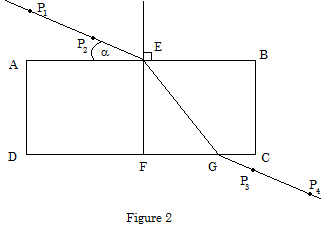
\includegraphics[width=10cm]{./img/2005-2-alt.png}
\end{center}

\textbf{Proceed as follows:}\\[10pt]

Place a white sheet of paper on the drawing board. Place the glass block, with one of its largest surfaces top most on top of the white paper. Mark the outline of the glass block on the paper with a pencil. Then remove the glass block and draw a line which cuts its largest sides normally at E and F as shown in figure 2 above. \\[10pt]

Using a protractor draw an angle $\alpha = 30^\circ$ with the glass block. Replace the glass block in its original position and stick the first pin P$_1$ and second pin P$_2$ along the line of angle $\alpha = 30^\circ$. Stick the third and fourth pins P$_3$ and P$_4$ respectively on the opposite side of the glass block such that P$_3$ and P$_4$ fall on a straight line with P$_1$ and P$_2$ when viewed through side CD of the glass block. \\[10pt]

Remove the glass block and trace the straight path taken by the ray G P$_3$ P$_4$. Using a ruler, join G and E. \\[10pt]

Measure the angle of refraction $r^\circ$, then calculate the values of $\cos{\alpha}$ and $\sin{r^\circ}$. Repeat the same procedure for values $\alpha = 40^\circ$, $50^\circ$, $60^\circ$, $70^\circ$ and $80^\circ$. Record your results in tabular form for the values of $\alpha$, $r^\circ$, $\sin{r^\circ}$ and $\cos{\alpha}$.

\begin{enumerate}
\item[(a)] Plot a graph of $\sin{r^\circ}$ (vertical axis) against $\cos{\alpha}$ (horizontal axis).
\item[(b)] Find the slope of the graph.
\item[(c)] Calculate the value of $C$ where slope = $\sin{C}$.
\item[(d)] State the possible sources of error and precautions you have taken during the experiment.
\end{enumerate}

\item[3.] The aim of this experiment is to determine the \textbf{e.m.f. E} and internal resistance \textbf{r} of a cell.

\begin{center}
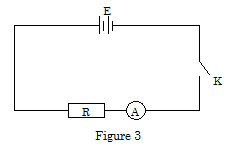
\includegraphics[width=7cm]{./img/2005-3-alt.png}
\end{center}

\begin{enumerate}
\item[(a)] Connect the circuit as shown in figure 3 above. Put $R = 1 \Omega$ and quickly read the value of $i$ on the ammeter.
\item[(b)] Repeat the procedure in 3 (a) above, for values of $R = 2 \Omega$, $3 \Omega$, $4 \Omega$ and $5 \Omega$ respectively.
\item[(c)] Tabulate your results and complete the following table.
\begin{center}
\begin{tabular}{|c|c|c|} \hline
\textbf{Resistance $R$ ($\Omega$)} & \textbf{Current $i$ (A)} & \textbf{$\cfrac{1}{i} \left(\text{A}^{-1}\right)$ } \\ \hline
1&& \\
2&& \\
3&& \\
4&& \\
5&& \\ \hline
\end{tabular} \\[10pt]
\end{center}
\item[(d)] Plot the graph of $R$ against $\cfrac{1}{i}$.
\item[(e)] The graph uses the equation $R = \cfrac{E}{i} - r$.
\begin{enumerate}
\item[(i)] Suggest how $E$ and $r$ may be evaluated from your graph.
\item[(ii)] Evaluate $E$ for one cell.
\item[(iii)] Evaluate $r$ for one cell.
\end{enumerate}
\item[(f)] State one source of error and suggest one way of minimizing it.
\end{enumerate}

\end{enumerate}
%\pagebreak
%\subsection{2004 - PHYSICS 2A ALTERNATIVE A PRACTICAL}

\begin{enumerate}
\item[1.] The aim of this experiment is to determine the mass of a given dry cell, size ``AA''.\\[5pt]

You are provided with a dry cell, a knife edge, two weights 50 g and 20 g, and a metre rule.\\[5pt]

Proceed as follows:
\begin{enumerate}
\item[(a)] Locate and note the centre of gravity C of the metre rule by balancing on the knife edge.
\item[(b)] Suspend the 50 g mass on one side of the metre rule, and 20 g together with the dry cell on the other side of the metre rule adjusting their position until the metre rule balances horizontally, as shown in Figure 1 below.

\begin{center}
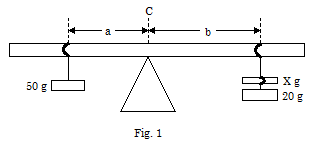
\includegraphics[width=10cm]{./img/2004-1-alt.png}
\end{center}

\item[(c)] By fixing a = 5 cm from C find its corresponding length, b, from C.
\item[(d)] Repeat and tabulate your results using a = 10 cm, 15 cm, 20 cm and 25 cm.
\item[(e)] Draw a graph of ``a'' against ``b'' and calculate its slope G.
\item[(f)] Calculate X from the equation $\text{G} = \cfrac{20 + \text{X}}{50}$. \hfill \textbf{(25 marks)}
\end{enumerate}


\item[2.] You are provided with a glass block, drawing board, optical pins and plane papers.\\

Place a white piece of paper on the drawing board. Place the glass block with one of its largest surface top most on top of the white paper. Mark the outline of the glass block on the paper with a pencil. Remove the glass block and draw a normal as shown in Figure 2 below.

\begin{center}
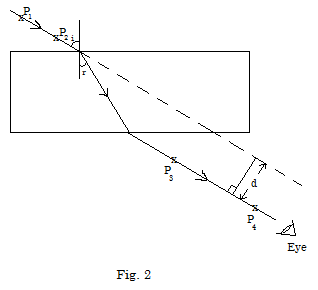
\includegraphics[width=10cm]{./img/2004-2-alt.png}
\end{center}

\begin{enumerate}
\item[(a)] Draw a line making an angle of incidence, $i$ of $30^\circ$. Erect two pins P$_1$ and P$_2$ on this line at a suitable distance apart. Replace the glass block and erect two more pins P$_3$ and P$_4$ at positions which appear to be in a straight line with the other two pins as seen through the glass block from the other side.\\[10pt]

Remove the glass block and draw the complete path of the ray (see Fig. 2). Measure the angle of refraction, $r$.
\item[(b)]
\begin{enumerate}
\item[(i)] Extend the direction of the incident ray as shown by the dotted line.
\item[(ii)] Measure the perpendicular distance `$d$' between extended incident ray and the emergent ray.
\end{enumerate}
\item[(c)] Repeat the procedure in (a) and (b) above for angles of incidence of $30^\circ$, $40^\circ$, $50^\circ$, $60^\circ$ and $70^\circ$. (In each case make your drawings on a fresh part of the drawing paper).
\item[(d)] Tabulate your results as shown in Table 1 below.
\begin{center}
\begin{tabular}{|p{0.15\textwidth}|p{0.15\textwidth}|p{0.15\textwidth}|p{0.15\textwidth}|p{0.15\textwidth}|} \hline
\multicolumn{1}{|c|}{$i$ (deg)} & \multicolumn{1}{c|}{$r$ (deg)} & \multicolumn{1}{c|}{$d$ (cm)} & \multicolumn{1}{c|}{$d\cos{r}$} & \multicolumn{1}{c|}{$\sin{(i-r)}$} \\ \hline
\multicolumn{1}{|c|}{30}&&&& \\
\multicolumn{1}{|c|}{40}&&&& \\
\multicolumn{1}{|c|}{50}&&&& \\
\multicolumn{1}{|c|}{60}&&&& \\
\multicolumn{1}{|c|}{70}&&&& \\ \hline
\end{tabular}\\[10pt]
\end{center}
\begin{enumerate}
\item[(i)] Plot a graph of $d\cos{r}$ against $\sin{(i-r)}$.
\item[(ii)] Find the gradient of the graph.
\item[(iii)] Measure the width of the glass block.
\item[(iv)] How is the gradient of the graph in 2 (a)(ii) and the width of the glass block in 2 (a)(iii) related?\\[5pt]
\end{enumerate}
\item[] NB: \quad Hand in your diagrams (drawings) together with your answer booklet. 
\item[] \flushright \textbf{(25 marks)}

\end{enumerate}

\item[3.] Determine the resistivity $\rho$ of the wire labelled W and the internal resistance of the battery provided.\\

Proceed as follows:

\begin{center}
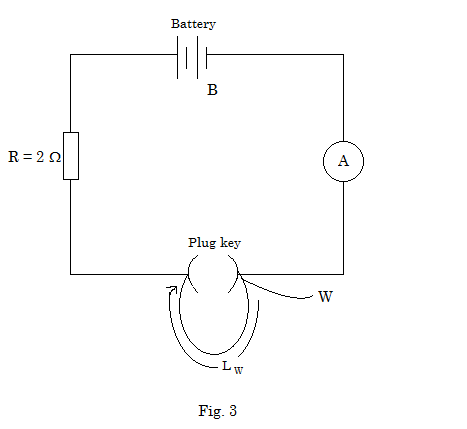
\includegraphics[width=10cm]{./img/2004-3-alt.png}
\end{center}

Connect the circuit as shown in fig. 3 above. With the plug key open adjust the length of wire W to a value of 20 cm. Note the ammeter reading.\\[10pt]

\noindent NB: The plug key should remain open throughout the experiment.

\begin{enumerate}
\item[(a)] Repeat the procedure above for $L_W$ = 40 cm, 60 cm, 80 cm and 100 cm each time recording the ammeter reading.
\item[(b)] Tabulate your results as shown in Table 2 below.

\begin{tabular}{|p{2.5cm}|c|c|} \hline
Length $L_W$ of wire (cm)& Current $I$ (A)& $\cfrac{1}{I} \left(\text{A}^{-1}\right)$ \\ \hline
&& \\
&& \\
&& \\
&& \\ \hline
\end{tabular}\\[10pt]

\item[(c)]
\begin{enumerate}
\item[(i)] Plot a graph of $\cfrac{1}{I}$ (vertical) against $L_W$ (horizontal).
\item[(ii)] Determine the slope G.
\item[(iii)] Determine the intercept $Y$ on the vertical axis.
\end{enumerate}
\item[(d)] Measure and record the diameter at four different places on the wire. Hence find the mean value of diameter $d$.
\item[(e)] Given that $G = \cfrac{4\rho}{\pi d^2E}$ and $Y = \cfrac{R + r}{E}$\\[10pt]
Where $E$ is the emf of the battery, and $R = 2 \Omega$, Find the
\begin{enumerate}
\item[(i)] Resistivity $\rho$ of the wire.
\item[(ii)]	Internal resistance $r$ of the battery. \hfill \textbf{(25 marks)}
\end{enumerate}
\end{enumerate}

\end{enumerate}
%\pagebreak
%\setcounter{secnumdepth}{2}
\settocdepth{section} % Return to default

% Part 6 - Science Activities and Competitions
\part{Science Activities and Competitions}
\label{prt:sci-activities}
\chapter{Hosting Science Events} \index{Science! events}

There are many great ways to promote math and science education through engaging activities for students and teachers alike. These can be done regularly through extracurricular clubs, but can also be organized together as part of a larger \emph{Science Day} event or multi-day \emph{Math and Science Conference}. What follow are some general tips and suggestions for hosting some of these various activities.

\section{Box of Fun} \index{Box of fun}
The \emph{Box of Fun} can be used as a teacher training exercise or as a student challenge. 
\begin{itemize}
\item Gather an assortment of everyday materials (see \nameref{cha:labequip}, p.~\pageref{cha:labequip}) and arrange them randomly across a table or in a large box. 
\item Ask participants to use the materials given to demonstrate some topic or principle in a subject of their choice (Biology, Chemistry, Physics or Math).
\item You may choose to put participants into groups and designate a specific subject for each group.
\item After at least 30 minutes, have groups come up to present their idea.
\item Additionally, you may ask groups to fill out an activity template (see \emph{Shika Express} companion manuals) to document their ideas.
\end{itemize}

The \emph{Box of Fun} is intended to foster participants' creativity and encourage them to see science in the world around them. Rather than thinking first of a topic and then deciding what materials are needed to show it, this activity encourages teachers to \emph{first look around and see what is available to them}, and then to think about how those things might be used to demonstrate some concept in science. \\

\noindent \textbf{CAUTION:} It may not be wise to assign specific topics to participants, as this can limit their creativity and may lead them to \emph{``destroy science''} by pretending a local substitute gives the same result as a traditional lab material when it really doesn't (e.g. pretending food colour is iodine because they have similar appearances). 

The purpose of using locally available materials is that they help to connect students to their everyday environment \emph{while still achieving the same results as expensive lab equipment}. However, if a local material does not give the same result, it should NOT be substituted merely for the sake of using local materials.

\section{Shika Express Gallery Walk} \index{Gallery walk}
This activity can be used to share ideas of science demonstrations among students and/or teachers.

\begin{itemize}
\item Choose 4-6 activities or demonstrations for each subject (see \emph{Shika Express} companion manuals for Biology, Chemistry, Physics and Math).
\item Prepare the demonstrations and arrange them across a set of tables, 1-2 tables per subject.
\item Spread the tables out evenly around a large empty room (e.g. dining hall).
\item Divide participants into equal groups based on the number of subjects being presented.
\item Have groups rotate among the different subject tables so that they are able to observe all demonstrations for each subject (approx. 15-20 mins per subject).
\item Following the rotations, give 20-30 mins to allow participants to return to a demonstration of their choice for further investigation or to construct it themselves.
\end{itemize}

\textbf{Suggestions:}
\begin{itemize}
\item You may wish to have 1-2 student or teacher leaders for each subject to help explain the demonstrations during the rotations. 
\item Write up brief explanation cards for each demonstration that participants can read as they walk by (or print activity write-ups from the \emph{Shika Express} manuals). 
\item Allow participants to perform the demonstrations themselves as much as possible, and then ask them to explain what they see.
\end{itemize}

%\section{Scientific Method Stations}
%Set up a series of 4-6 stations with activities focused on the use of the scientific method. Divide students into groups and have them rotate among the various activities.
%
%\textbf{Suggestions:}
%\begin{itemize*}
%\item[] Biology
%	\begin{itemize*}
%	\item Lung Capacity
%	\end{itemize*}
%\end{itemize*}

\section{Science Fair} \index{Science! fair}
\emph{Science Fair} projects provide a great opportunity for students to apply their knowledge and investigate their interests in science.

\begin{itemize}
\item Have interested students form groups of 2-3.
\item Groups select a project idea based on a shared interest or question/problem to address. Encourage students to think about what problems or issues are faced in their own communities. 
%(For ideas, see suggestions below.)
%\nameref{cha:sci-fair-projects})
\item Review the steps of the Scientific Method. Have students identify the problem and form a hypothesis for their project.
\item Allow several weeks for groups to work on their projects (provide additional books or computer resources if available).
\item When completed, allow students to set up and explain the various projects around the school for all students to see.
\item Encourage students to apply to participate in the national \href{www.youngscientists.co.tz}{Young Scientists Tanzania (YST)} competition (\url{www.youngscientists.co.tz}) in Dar es Salaam.
\end{itemize}

%\subsection{Project Ideas}
%See the \emph{Shika Express} companion manuals for more information on these and many other ideas.
%\begin{itemize*}
%\item Biology:
%	\begin{itemize*}
%	\item Digestive system model (using local materials)
%	\item Human skeleton model
%	\item Plant and animal cell models / displays
%	\item Classification of specimens
%	\end{itemize*}
%\item Chemistry:
%	\begin{itemize*}
%	\item Production of carbon dioxide gas (vinegar and baking soda)
%	\item Effects of chemicals on soil pH
%	\item Requirements for rusting
%	\end{itemize*}
%\item Physics:
%	\begin{itemize*}
%	\item Sustainable energy sources (windmill, water wheel, etc.)
%	\item Simple electric circuit
%	\item Simple machines
%	\end{itemize*}	
%\end{itemize*}

%\subsection{Display Ideas}
%\begin{center}
%\includegraphics[width=10cm]{./img/}
%\end{center}

\section{Science Competitions} \index{Science! competitions}
Perform individual competitions or many strung together over the course of a day or weekend. 

For more, see the section on \nameref{cha:sci-comp} (p.~\pageref{cha:sci-comp}).

\section{Science Day} 
Engage the entire school (or multiple schools) by combining several activities into a \emph{Science Day} event.

\begin{itemize}
\item Invite a guest speaker to speak on career opportunities in math and science (e.g. accountant, engineer, doctor, nurse, carpenter, mechanic, store owner, etc.)
\item Explain applications of math and science in all walks of life (e.g. farming, buying/selling, health/disease, transport, weather, drinking water, football, etc.)
\item Incorporate \emph{\nameref{cha:sci-comp}} - elect 1 or 2 teams from each Form to compete, with the rest of the school as an audience.
\item Incorporate \emph{Box of Fun} and \emph{Gallery Walk} activities. It may be helpful to do the \emph{Gallery Walk} first to provide examples to participants.
\item Encourage girls' empowerment wherever possible.
\item Give out a survey to gauge students' perception of science.
\end{itemize}

A \emph{Science Day} event may not guarantee immediate improvements in test scores, but it shows students that \emph{the school and its teachers are not willing to give up on math and science, and neither should they!} Continued promotion of math and science will help to change students' perception of the subjects that they may initially write off as being too difficult. Excitement and interest is the first step in changing that perception.

\section{Math and Science Conferences} \index{Science! conferences}
Gather students from several nearby schools to hold a special week-long \emph{Math and Science Conference} in a nearby town or at a host school.

In addition to those ideas presented for a \emph{Science Day} event,
\begin{itemize}
\item Incorporate HIV/AIDS and malaria into science demonstrations/activities (see \emph{Shika Express} companion manuals for ideas).
\item Have students prepare \emph{Science Fair} projects over the course of the conference and present on the final day.
\item Give award certificates for participation and prizes for individual/team competitions.
\end{itemize}

\emph{Math and Science Conferences} encourage leadership among their participants. Students attending such events are likely to be good \emph{ambassadors of science}, sharing what they have done and learned with fellow students back at school. Those students may then try to improve their own performance in those subjects so that they can attend a similar event later on.

\section{Teacher Trainings} \index{Teacher trainings}

Conferences can also be directed towards improving teacher performance by conducting the suggested activities at a nearby Teacher's College. 
\chapter{Science Competitions} \index{Science! competitions}
\label{cha:sci-comp}
\setcounter{secnumdepth}{0}

Students, just like nearly all other people, enjoy competing against one another. Likening math and science-related activities to the competition of a football league can be a wonderful motivator for students. Given below are some suggestions for utilizing competitions while teaching about science.

\begin{itemize}
\item Combine students of various abilities together on a team. This will allow the bright students to develop leadership skills and help to bring up the slow learners.
\item Limit teams to 3-5 students. Balance the number of boys and girls on a team, or choose to have all-boys teams compete against all-girls teams.
\item Allow students to pick their own team name, and possibly draw a team flag if time allows.
\item Create a standings board for the competition. For example:\\

\begin{table}[h!]
	\centering
		\begin{tabular}{|l|l|l|l|l|l||l|}\hline
		& \rotatebox{90}{
		\begin{tabular}{l}
		Egg Drop
		\end{tabular}
		}
		& \rotatebox{90}{
		\begin{tabular}{l}
		Jenga Jengo
		\end{tabular}
		}
		& \rotatebox{90}{
		\begin{tabular}{l}
		Raft Rally
		\end{tabular}
		}
		& \rotatebox{90}{
		\begin{tabular}{l}
		Drop Zone
		\end{tabular}
		}
		& \rotatebox{90}{
		\begin{tabular}{l}
		Bridge Challenge
		\end{tabular}
		}
		& \rotatebox{90}{
		\begin{tabular}{l}
		\textbf{Total}
		\end{tabular}
		} \\ \hline
		Big Stars &&&&&&\\ \hline
		Chelsea &&&&&&\\ \hline
		Simba &&&&&&\\ \hline
		Arsenal &&&&&&\\ \hline
		Kings &&&&&&\\ \hline
		Manchester United &&&&&&\\ \hline
		\end{tabular}
\end{table}

\item Have teams present and explain their designs to the audience where applicable. Allow other students to ask questions/provide criticisms.
\item Follow up each activity with a short lesson about a concept illustrated by the competition (e.g. Archimedes' Principle for \emph{Raft Rally}; see competition write-ups for more).
\item Ask students how they would revise their designs or make improvements if they could do the activity again.
\item Explain how the activities can be applied to solve real-life problems (e.g. \emph{Jenga Jengo} for Civil Engineers).
\end{itemize}

\vfill
\pagebreak

%=================================================================================================%

\section{Egg Drop} \index{Egg drop}
\label{sec:egg-drop}


\textbf{Time:} 1 hour

\subsection{How It Works}
Students must build a device to transport an egg through a given drop distance without cracking.

\subsection{What You Need (per team)}
\begin{tabular}{p{0.33\textwidth} p{0.33\textwidth} p{0.33\textwidth}}
$\Box$ Plain paper – 4 sheets	&	$\Box$ Straws – 10		&	$\Box$ Paper clips - 10 \\
$\Box$ Plastic bag - 2		&	$\Box$ Toothpicks – 10		&	$\Box$ Toilet paper – 1 roll \\
$\Box$ String – 1 metre	&		$\Box$ Tongue depressors – 4	&	$\Box$ Bottle (500 ml) - 1 \\
$\Box$ Masking tape – 1 roll	&	$\Box$ Rubber bands – 4	&		$\Box$ Newspaper – 1 sheet \\
$\Box$ Balloons – 4		&	$\Box$ Index cards – 4		&	$\Box$ Egg – 1
\end{tabular}

\subsection{Rules}
\begin{itemize*}
\item 45 minute time limit for construction.
\item Devices dropped from a height of 3-5 metres.
\item Teams can use only the materials given, but do not need to use everything.
\item Egg is placed at time of testing.  It must be possible to place and remove egg freely without altering the device.
\item Once egg is placed, no further adjustments may be made. This means the egg cannot have any kind of ``seat belt'' or strap fastened after placing the egg.
\end{itemize*}

\subsection{Points}
Egg Survives - 50 pts \quad Egg Cracks - 0 pts

\subsection{Additional Materials}
\begin{itemize*}
\item Ladder / chair
\item Scissors for community use
\end{itemize*}

\subsection{Notes}
\begin{itemize*}
\item Do not give eggs to teams until time of testing.
\item If possible, increase drop height for surviving eggs and give bonus 25 pts for each additional successful drop.
\end{itemize*}

\subsection{Science Applications}
\begin{description}
\item[Air Resistance (Physics Form I):]{Air resistance provides a frictional force which opposes the object's motion as gravity attracts it towards the centre of the earth. This upward force reduces the speed of the object as it falls, allowing it to land more softly and protect the egg. Thus, we want to maximize the air resistance on the object (e.g. by using a large parachute).}
\item[Pressure (Physics Form I):]{The force of impact on the device when it hits the ground can be reduced by increasing the surface area which contacts the ground. Constructing a wide base (e.g. using balloons) reduces the impact on the egg and thus helps to protect it.}
\end{description}

\subsection{Taking It Further}
Did students utilize the parachute concept? If not, show a brief example. How does this help to protect the egg? Is it better to have a large parachute or a small one?

\pagebreak

%=================================================================================================%

\section{Jenga Jengo} \index{Jenga Jengo}
\label{sec:jenga-jengo}


\textbf{Time:} 30-45 minutes

\subsection{How It Works}
Students must build the tallest structure possible, using only paper and tape, as quickly as possible and while ensuring good stability.

\subsection{What You Need (per team)}
$\Box$ Plain paper – 25 sheets\\
$\Box$ Masking tape – 1 roll

\subsection{Rules}
\begin{itemize*}
\item 20-minute time limit for construction.
\item Cannot use tape roll as weight inside structure.
\item Stability tested by waving book at structure (Wind Test).
\end{itemize*}

\subsection{Points}
1$^{st}$ to finish – 50 pts\\
Tallest structure – 50 pts\\
Passes Wind Test – 50 pts

\subsection{Additional Materials}
\begin{itemize*}
\item Tape Measure
\item Stopwatch
\item Book / waving device
\end{itemize*}

\subsection{Notes}
\begin{itemize*}
\item All structures that pass the Wind Test are awarded 50 pts.
\item Alternate Wind Test: place structures outside on a windy day. Those standing after 1 minute pass.
\end{itemize*}

\subsection{Science Applications}
\begin{description}
\item[Centre of Gravity (Physics Form I):]{Civil engineers construct buildings with a low centre of gravity, making them less likely to fall over due to wind forces. To maintain \emph{stable equilibrium}, a building should have a wide base with a large mass, while the top of the building should have a small area and less mass.}
\end{description}

\subsection{Taking It Further}
\begin{itemize*}
\item Show students pictures of buildings and structures from around the world after the competition. Did the students’ structures resemble any of them?
\item Try variations, giving students index cards, straws or matches instead of plain paper.
\end{itemize*}

\pagebreak

%=================================================================================================%

\section{Raft Rally} \index{Raft Rally}
\label{sec:raft-rally}


\textbf{Time:} 30-45 minutes

\subsection{How It Works}
Students must build a raft using only aluminum foil that can support the heaviest load before sinking.

\subsection{What You Need (per team)}
$\Box$ Aluminum foil – 20 cm $\times$ 20 cm sheet\\
$\Box$ Straws - 4 (optional)

\subsection{Rules}
\begin{itemize*}
\item 10-minute time limit for construction.
\item Replacement sheet may be given in case of rips/tears, at a 20 pt deduction.
\end{itemize*}

\subsection{Points}
1$^{st}$ Place – 100 pts \\
2$^{nd}$ Place – 75 pts \\
3$^{rd}$ Place – 50 pts \\
4$^{th}$ Place – 25 pts \\
Others – 0 pts

\subsection{Additional Materials}
\begin{itemize*}
\item Large container or bucket (clear if possible) filled with water
\item Nails ($\times$ 200) / Bottle caps ($\times$ 200) / Other small weights for testing
\end{itemize*}

\subsection{Notes}
\begin{itemize*}
\item As raft approaches the point of sinking, add weights more slowly.
\item Raft is finished when water begins to enter, and total number of weights is recorded.
\end{itemize*}

\subsection{Science Applications}
\begin{description}
\item[Archimedes' Principle (Physics Form I):]{\emph{Archimedes' Principle} states that $$\mathrm{Upthrust} = \text{Weight of displaced fluid}$$
Here, we want to maximize the force of upthrust to avoid sinking. So that means maximize the Weight of the displaced water: $\mathrm{Weight} = \mathrm{mass} \times \text{acceleration due to gravity}$, or					 $$W=mg$$
Gravity is a constant , but mass depends on 2 things: density ($\rho$) and volume ($V$). We know that
$\rho = \frac{m}{V}$, so that means				           $$m = \rho V$$
The density of the water is constant, so the only thing we can change is the \emph{Volume} of water displaced. Thus to get the most upthrust and prevent sinking, we need to displace a large volume of water, i.e. build a raft with a large base.}
\end{description}

\subsection{Taking It Further}
\begin{itemize*}
\item Ask students how they would revise their designs if they could do it again.
\item Try variations, giving students straws, toothpicks, tongue depressors or index cards.
\end{itemize*}

\pagebreak

%=================================================================================================%

\section{Drop Zone} \index{Drop Zone}
\label{sec:drop-zone}


\textbf{Time:} 30-45 minutes

\subsection{How It Works}
Students must build a parachute using limited materials to carry a paper clip passenger as close as possible to a target, while maximizing hang time.

\subsection{What You Need (per team)}
\begin{tabular}{p{0.33\textwidth} p{0.33\textwidth} }
$\Box$ Paper clip – 1	&		$\Box$ Plastic bag - 2 \\ 
$\Box$ String – 1 metre		&	$\Box$ Plain paper – 2 sheets \\ 
$\Box$ Masking tape – 15 cm	&	$\Box$ Scorecard (see example below) \\ 
\end{tabular}

\subsection{Rules}
\begin{itemize*}
\item 10-15 minute time limit for construction.
\item Parachutes dropped from a height of 3-5 metres.
\item Average hang time and distance from target taken over 3 trials for each team.
\end{itemize*}

\subsection{Points}
\begin{tabular}{llllll}
Hang Time (Longest):& 1$^{st}$ – 50 pts,&	2$^{nd}$ – 35 pts,&	3$^{rd}$ – 20 pts,& 	4$^{th}$ – 5 pts,& 	Others – 0 pts\\
Distance (Shortest):& 1$^{st}$ – 50 pts,&	2$^{nd}$ – 35 pts,&	3$^{rd}$ – 20 pts,& 	4$^{th}$ – 5 pts,& 	Others – 0 pts
\end{tabular}

\subsection{Additional Materials}
\begin{tabular}{p{0.3\textwidth} p{0.3\textwidth}} \\[-30pt]
\begin{itemize*}
\item Tape measure		
\end{itemize*}	& \begin{itemize*}
\item Flipchart target
\end{itemize*}\\[-30pt]
\begin{itemize*}
\item Stopwatch	
\end{itemize*}	& \begin{itemize*}
\item Ladder / chair
\end{itemize*}\\[-10pt]
\end{tabular}

\subsection{Notes}
\begin{itemize*}
\item Scorecard:
\end{itemize*}
\begin{tabular}{|l|c|c|c|c|c|} \hline
\textbf{Team:} & \textbf{Trial 1} & \textbf{Trial 2} & \textbf{Trial 3} & \textbf{Average} & \textbf{Points} \\ \hline
\textbf{Hang Time (s)} & & & & & \\ \hline
\textbf{Distance from Target (cm)} & & & & & \\ \hline
\end{tabular}
\begin{itemize*}
\item Measure distance from paper clip to centre of target.
\end{itemize*}

\subsection{Science Applications}
\begin{description}
\item[Air Resistance (Physics Form I):]{Air resistance provides an upward force on the parachute, which acts against the force of gravity and causes the object to fall more slowly. The larger the surface area of the parachute, the more slowly it will fall.}
\end{description}

\subsection{Taking It Further}
\begin{itemize*}
\item Students may not be familiar with parachutes. Prepare a simple example to explain the concept and function.
\item Ask students questions: Why does the parachute slow the object down? To maximize hang time, do we want a very large or very small parachute? Would a parachute work on the moon?
\item Drop parachute side-by-side with a paper clip having no parachute. Which one made it safely?
\end{itemize*}

\pagebreak

%=================================================================================================%

\section{Bridge Challenge} \index{Bridge Challenge}
\label{sec:bridge-challenge}


\textbf{Time:} 1 hour 30 minutes

\subsection{How It Works}
Students must build a bridge that can support the most weight, while using a limited budget of \emph{\nameref{cha:sci-shillings}} to purchase construction materials.

\subsection{What You Need (per team)}
\begin{tabular}{p{0.3\textwidth} p{0.3\textwidth} p{0.4\textwidth}}
$\Box$ Straws - 20		&	$\Box$ String – 3 m	&	$\Box$ Masking tape – 1 roll\\
$\Box$ Bamboo skewers - 20	&	$\Box$ Office glue – 1 tube	& $\Box$ Duct tape – 1 roll (total)\\
$\Box$ Bamboo stick (fimbo) – 1	&	$\Box$ Rubber bands - 10	&	$\Box$ Ruler - 1\\
$\Box$ Tongue depressors – 10	&	$\Box$ Pencils - 2		&	$\Box$ Scissors - 1\\
$\Box$ Toothpicks – 2 small cans	&	$\Box$ Index cards – 10	&	$\Box$ \nameref{cha:sci-shillings} – 20 (see p. \pageref{cha:sci-shillings})
\end{tabular}

\subsection{Rules}
\begin{itemize*}
\item Approximately 45 minute time limit for construction.
\item Teams begin with only a ruler, scissors and 20 \emph{Science Shillings}. These items may NOT be used in construction of bridge.
\item All building materials must be purchased from a science shop. Suggested prices are as follows:\\

\begin{tabular}{p{0.25\textwidth} p{0.1\textwidth} p{0.25\textwidth} p{0.1\textwidth}}
Straws (bundle of 10)	& 1 /=	&	Office glue (1 tube)	&	3 /=\\
Skewers (bundle of 10) &	2 /=	&	Rubber bands ($\times$ 5)	&	1 /=\\
Fimbo		&		3 /=	&	Pencil 		&		1 /=\\
Tongue depressors ($\times$ 5)	 & 2 /=	&	Index cards ($\times$ 5)	&	1 /=\\
Toothpicks (2 small cans) &	1 /=	&	Masking tape (1 roll)	&	3 /=\\
String (1 metre)	&	1 /=	&	Duct tape (30 cm)	&	1 /=\\[10pt]
\end{tabular}

\item Bridges will be loaded by placing rocks or other weights into a small bucket that must rest on top of the bridge.
\item Bridge must span a 30 cm gap between two chairs / tables.
\item 1 student from each team must be designated as team accountant. Only this student may purchase items from the shop.
\end{itemize*}

\subsection{Points}
(Based on number of rocks / weights placed before bridge fails)\\
1$^{st}$ – 100 pts, \quad	2$^{nd}$ – 75 pts, \quad	3$^{rd}$ – 50 pts,\quad 	4$^{th}$ – 25 pts,\quad 	Others – 0 pts\\
\textbf{BONUS}: 5 pts per \emph{Science Shilling} remaining after construction

\subsection{Additional Materials}
\begin{tabular}{p{0.5\textwidth} p{0.5\textwidth}} \\[-30pt]
\begin{itemize}
\item Small bucket 		
\end{itemize}	& \begin{itemize}
\item Science shop table
\end{itemize}\\[-30pt]
\begin{itemize*}
\item Several large rocks (20) / other large weights 		
\end{itemize*}	& \begin{itemize*}
\item Extra bamboo sticks (fimbos) – 2-4
\end{itemize*}\\[-30pt]
\begin{itemize*}
\item 2 chairs / tables 30 cm apart		
\end{itemize*}	& \begin{itemize*}
\item Index Cards for price signs – 12
\end{itemize*}\\[-10pt]
\end{tabular}

\subsection{Notes}
\begin{itemize*}
\item Student accountants may only purchase 1 of each item at a time. They must allow other students to make purchases before buying another of that item.
\item At some point 15-20 minutes into construction time, shopkeeper may announce a newly received shipment of bamboo sticks (fimbos). However, due to demand, the price has increased to 5 /=.
\item Bridge has failed when it either collapses / breaks or when the bucket can no longer be balanced on top of it. Record largest number of weights successfully added.
\end{itemize*}

%\subsection{Science Applications}
%\begin{description}
%\item[]{}
%\end{description}

\subsection{Taking It Further}
\begin{itemize*}
\item Ask students to present their bridges and describe how they decided to manage their money. What materials did they purchase and why?
\item What would they do differently if they could start again?
\item Which team finished with the most total points after the \textbf{BONUS}? Did the most money spent result in the strongest bridge? Who was the most \emph{efficient} with their money?
\item Show students pictures of bridges from around the world after the competition. Did the students’ bridges resemble any of them?
\end{itemize*}

%\pagebreak

%=================================================================================================%

%\section{Paper Airplanes}

%=================================================================================================%

%\section{Card Tower}

%=================================================================================================%

%\section{Write It, Do It}

%=================================================================================================%


\chapter{The Scientific Procedure}

The following activities can be used as a method of introducing students to the scientific method. Rather than just performing the activities, first identify the question or problem with the students, then have them form a hypothesis for each step of the experiment. Students should record observations and data accordingly and use them to draw a conclusion about the activity.

Prepare an activity sheet for each student or have them copy it into their notebooks before performing the activities. Set up stations for the various activities and have students rotate among them in small groups.

After performing several of the experiments, ask students to come up with their own. Ask them to think about problems they face in their daily lives. Encourage interested students to turn their ideas into a science fair project to display for the school or community.

%==================================================================================================%

\section{Biology}


\subsection{Hand Washing}

%\begin{center}
%\includegraphics[width=0.4\textwidth]{./img/source/.jpg}
%\end{center}

\begin{description*}
\item[Materials:]{Soap, water, bottle, basin/bucket, chalk, charcoal, food colour, stopwatch}
\item[Setup:]{Prepare a large amount of soapy water. Grind the chalk and charcoal into separate powders.}\\
\item[Problem:]{How long should we wash our hands?\\

\begin{tabular}{|l|c|c|} \hline
\multirow{2}{*}{\textbf{Material}} & \textbf{Hypothesis} & \multirow{2}{*}{\textbf{Experimental Result}} \\
& \textbf{(Seconds)} & \\ \hline
Chalk powder & & \\ \hline
Charcoal powder & & \\ \hline
Food colour & & \\ \hline
\end{tabular} \\[10pt]
}\\
\item[Hypothesis:]{Predict how much time it will take to completely clean your hands and record in the table.}
\item[Procedure:]{Start a stopwatch and have a student or teacher slowly pour soapy water over a basin while the student washes his or her hands. Stop the clock when the student's hands are completely clean.}
\item[Observations:]{Record the time taken to completely wash your hands in the table.}
\item[Questions:]{}\hfill
\begin{enumerate}
\item Why is it important to wash our hands?
\item When do we need to wash our hands?
\end{enumerate}
\item[Theory:]{Washing our hands with soap and water helps to kill harmful bacteria that can cause us to become sick if allowed into our bodies. It is very important to wash our hands before eating and after using the bathroom.}
\end{description*}

\pagebreak


\subsection{Lung Capacity}

\begin{center}
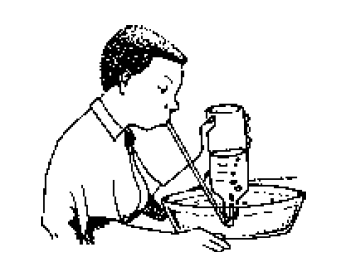
\includegraphics[width=0.4\textwidth]{./img/source/lung-capacity.png}
\end{center}

\begin{description*}
\item[Materials:]{1.5 L bottle, basin, water, plastic tubes/straws, soap, marker, ruler}
\item[Setup:]{Make a scale on the bottle using a marker and ruler (e.g. 100 mL increments). Prepare a soap solution for washing the tubes/straws}\\
\item[Problem:]{How much air can your lungs hold?\\

\begin{tabular}{|l|c|c|} \hline
\multirow{2}{*}{\textbf{Breath}} & \textbf{Hypothesis} & \multirow{2}{*}{\textbf{Experimental Result}} \\
& \textbf{(Volume of air in mL)} & \\ \hline
Normal breath & & \\ \hline
Full breath & & \\ \hline
After holding breath for 10 seconds & & \\ \hline
\end{tabular} \\[10pt]
}
\item[Hypothesis:]{Record the volume of air that you think the lungs can hold for each case in the table.}
\item[Procedure:]{Fill a basin with water. Fill a 1.5 L bottle with water and invert it in the basin so that the mouth of the bottle is underneath the water. Place one end of the tube/straw inside the bottle under water. For each breath, blow into the tube to displace the water.}
\item[Observations:]{Note the reading on the scale before and after blowing into the tube and record the \emph{difference} to give the amount of water displaced.}
\item[Questions:]{}\hfill
\begin{enumerate}
\item Which breath produces the largest amount of air? Which give the smallest amount?
\item How long can you hold your breath?
	\begin{enumerate}
	\item[] Hypothesis: I can hold my breath for \_\_\_\_\_\_\_ seconds.
	\item[] Experimental Result: I can hold my breath for \_\_\_\_\_\_\_ seconds.
	\end{enumerate}
\end{enumerate}
\item[Theory:]{When we breath in air, our bodies use the oxygen and produce carbon dioxide in a process called \emph{respiration}. Oxygen is transported in our blood throughout our bodies. When we hold our breath, oxygen is not circulated throughout our bodies and we begin to feel lightheaded.}
\end{description*}

\pagebreak


%==================================================================================================%

\section{Chemistry}


\subsection{Acids and Bases}

\begin{center}
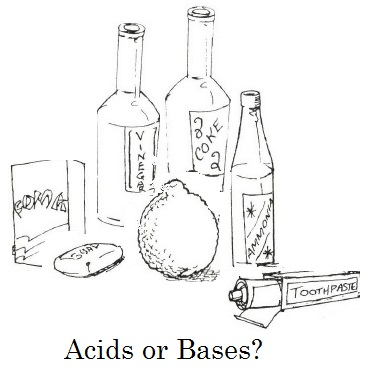
\includegraphics[width=0.4\textwidth]{./img/source/acids-bases-sci-meth.jpg}
\end{center}

\begin{description*}
\item[Materials:]{Bottles, bottle caps, water, vinegar, lemons, baking soda, soda, soap, antacid tablets, rosella leaves, straws/syringes}
\item[Setup:]{Prepare solutions for each of the items above in separate bottles. Prepare indicator by placing rosella leaves in hot water.}\\
\item[Problem:]{What differences can we observe among acids and bases?\\

\begin{tabular}{|l|c|c|} \hline
\multirow{2}{*}{\textbf{Solutions}} & \textbf{Hypothesis} & \multirow{2}{*}{\textbf{Experimental Result}} \\
& \textbf{(Which is different?)} & \\ \hline
Vinegar, lemon, baking soda & & \\ \hline
Vinegar, baking soda, soap & & \\ \hline
Baking soda, antacid, soda & & \\ \hline
Soda, soap, vinegar & & \\ \hline
\end{tabular} \\[10pt]
}
\item[Hypothesis:]{For each set of solutions, which one will reveal a colour different from the others? Record your predictions in the table.}
\item[Procedure:]{Place small amounts of 3 different solutions in separate bottle caps according to the table. Add a few drops of rosella indicator to each.}
\item[Observations:]{Record observations of colour change under \emph{Experimental Result} in the table.}
\item[Questions:]{\hfill
\begin{enumerate}
\item Which solutions have similar properties?
\item Which solutions are acids? What colour do they show?
\item Which solutions are bases? What colour do they show?
\end{enumerate}
}
\item[Theory:]{Coloured leaves such as rosella act as indicators for identifying acids and bases. Adding rosella indicator reveals a red colour for acids and a blue colour for bases. Students do not need to understand the differences between acids and bases in order to observe their different behaviours. Locally available examples of acids include sour milk, citrus fruits and soda. Local bases include ammonia, toothpaste and detergent.}
\end{description*}

\pagebreak

\subsection{Mixing Acids and Bases}

\begin{center}
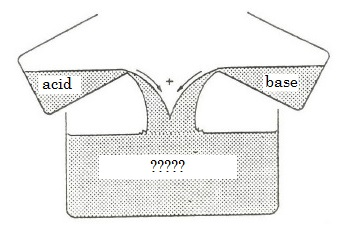
\includegraphics[width=0.6\textwidth]{./img/source/mixing-acid-base.jpg}
\end{center}

\begin{description*}
\item[Problem:]{What happens when acids and bases are mixed together?\\

\begin{tabular}{|l|c|c|} \hline
\multirow{2}{*}{\textbf{Solutions to Mix}} & \textbf{Hypothesis} & \multirow{2}{*}{\textbf{Experimental Result}} \\
& \textbf{(What colour?)} & \\ \hline
Mix vinegar and lemon & & \\ \hline
Mix baking soda and soap & & \\ \hline
Mix vinegar and baking soda & & \\ \hline
\end{tabular}\\[10pt]
}
\item[Hypothesis:]{Predict any colour changes or observations when pairs of solutions are mixed together. Record in the table.}
\item[Procedure:]{Mix small amounts of solutions together according to the table.}
\item[Observations:]{Record observations (colour changes, etc.) in the table.}
\item[Questions:]{\hfill
\begin{enumerate}
\item What happens when an acid is mixed with an acid?
\item What happens when a base is mixed with a base?
\item What happens when an acid is mixed with a base?
\end{enumerate}
}
\item[Theory:]{Mixing acids with acids and bases with bases may cause the colour of the solution to turn darker or lighter depending on the solutions used. Mixing an acid with a base should reveal a colourless solution and produce carbon dioxide gas. You may need to vary the amounts of acid and base to get a colourless solution depending on their concentrations.}
\end{description*}

\pagebreak


%\subsection{Separation of Mixtures}
%
%%\begin{center}
%%\includegraphics[width=0.4\textwidth]{./img/source/.jpg}
%%\end{center}
%
%\begin{description*}
%\item[Materials:]{Bottles, salt, water, rice, beans, steel wool, paper, cloth, oil, wire mesh (sieve), sand, maize seeds, magnet}
%\item[Setup:]{}\\
%\item[Problem:]{\\
%
%\begin{tabular}{|l|c|c|} \hline
%\multirow{2}{*}{\textbf{Mixture}} & \textbf{Hypothesis} & \multirow{2}{*}{\textbf{Experimental Result}} \\
%& \textbf{(Filtration, Decantation, Distillation, Chromatography, Magnet)} & \\ \hline
%Water and sand& & \\ \hline
%& & \\ \hline
%\end{tabular} \\[10pt]
%}\\
%\item[Hypothesis:]{}
%\item[Procedure:]{}
%\item[Observations:]{}
%\item[Questions:]{}\hfill
%\begin{enumerate}
%\item 
%\end{enumerate}
%\item[Theory:]{}
%\end{description*}

%==================================================================================================%

\section{Physics}


\subsection{Complete the Circuit}

\begin{center}
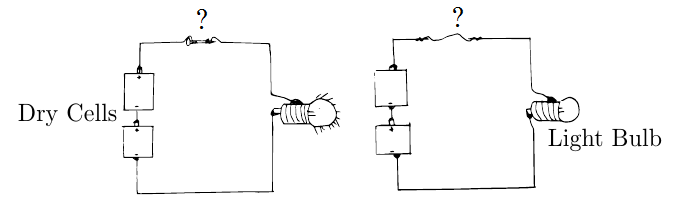
\includegraphics[width=0.8\textwidth]{./img/conductors-insulators-sci-meth.png}
\end{center}

\begin{description*}
\item[Materials:]{Dry cell, speaker wire, bulb/ammeter, cardboard, various objects, e.g. rubber band, nail, paper, aluminum foil, toothpick, pen, scissors, bottle cap, coin, balloon, chalk}
\item[Setup:]{Connect a dry cell and bulb in series using speaker wire and attach to a sheet of cardboard. Leave two wires free and pin to the cardboard to act as a switch.}
\item[Problem:]{Which objects will light a bulb?\\

\begin{tabular}{|l|c|c|} \hline
\multirow{2}{*}{\textbf{Object}} & \textbf{Hypothesis} & \multirow{2}{*}{\textbf{Experimental Result}} \\
& \textbf{(Light or No Light)} & \\ \hline
Copper wire & & \\ \hline
Pen & & \\ \hline
Aluminum foil& & \\ \hline
Paper& & \\ \hline
Nail& & \\ \hline
Toothpick& & \\ \hline
Bottle cap& & \\ \hline
Balloon& & \\ \hline
Chalk& & \\ \hline
Scissors (blade)& & \\ \hline
Scissors (handle)& & \\ \hline
\end{tabular}\\[10pt]
}
\item[Hypothesis:]{Predict which materials will cause the bulb to light when placed across the switch. Record predictions in the table.}
\item[Procedure:]{Test each object by placing it across the free wires to close the circuit.}
\item[Observations:]{Record the result for each item in the table.}
\item[Questions:]{}\hfill 
\begin{enumerate}
\item Which materials caused the bulb to light?
\item These objects are made from what kind or materials?
\item What other objects in the room can you find to test? Will they light the bulb?
\end{enumerate}
\item[Theory:]{\emph{Conductors} are materials which easily allow electrons to flow through them. \emph{Insulators} are materials which do not easily allow the the flow of electrons. Examples of good conductors are most metals, water and the human body. Examples of good insulators are rubber, wood and plastic.}
\end{description*}

\pagebreak


\subsection{Density Tower}

\begin{center}
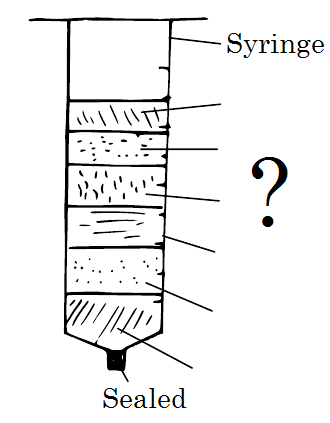
\includegraphics[width=0.3\textwidth]{./img/density-tower-sci-meth.png}
\end{center}

\begin{description*}
\item[Materials:]{Syringes, bottles, water, cooking oil, kerosene, spirit, honey, glycerine, tape, scissors}
\item[Setup:]{Prepare a test tube rack by cutting a bottle and filling it with dirt. Remove the plungers from the syringes and seal them with tape, super glue, or by melting to opening closed.}\\
\item[Problem:]{Which liquids are more dense than others?\\

\begin{tabular}{|l|c|c|} \hline
\multirow{2}{*}{\textbf{Liquid}} & \textbf{Hypothesis} & \multirow{2}{*}{\textbf{Experimental Result}} \\
& \textbf{(Position, 1 = bottom)} & \\ \hline
Water & & \\ \hline
Cooking oil & & \\ \hline
Kerosene & & \\ \hline
Spirit & & \\ \hline
Honey & & \\ \hline
Glycerine & & \\ \hline
\end{tabular} \\[10pt]
}\\
\item[Hypothesis:]{Predict the order in which the liquids will settle from the bottom of the syringe. Assign 1 to the bottom liquid, 2 to the one above it, and so on.}
\item[Procedure:]{Pour a small amount of each liquid into a syringe, observing after each addition.}
\item[Observations:]{After adding all liquids, record the order in which they rest, starting with 1 at the bottom.}
\item[Questions:]{}\hfill
\begin{enumerate}
\item Which liquid finished at the bottom?
\item Which liquid finished at the top?
\item Which liquid has the greatest density?
\item Which liquid has the lowest density?
\item What happens if you place a small object (e.g. paper clip, eraser, paper) in the tower? 
\end{enumerate}
\item[Theory:]{\emph{Density} is a property of different materials and liquids. It is a ratio of its mass to its volume. Dense liquids sink to the bottom, while less dense liquids rise to the top. A small object placed in the tower will settle in the liquid which is nearest its own density.}
\end{description*}

\pagebreak


\subsection{Sinkers and Floaters}

%\begin{center}
%\includegraphics[width=0.4\textwidth]{./img/source/.jpg}
%\end{center}

\begin{description*}
\item[Materials:]{Basin of water, various objects, e.g. nail, paper clip, paper, aluminum foil, soda cap, matchbox, pen cap, toothpick, balloons, flour}
%\item[Setup:]{}\\
\item[Problem:]{Which objects sink or float when placed in water?\\

\begin{tabular}{|l|c|c|} \hline
\multirow{2}{*}{\textbf{Object}} & \textbf{Hypothesis} & \multirow{2}{*}{\textbf{Experimental Result}} \\
& \textbf{(Sink or Float)} & \\ \hline
Nail& & \\ \hline
Paper clip& & \\ \hline
Pen cap& & \\ \hline
Soda cap (dropped)& & \\ \hline
Soda cap (placed carefully)& & \\ \hline
Toothpick & & \\ \hline
Paper& & \\ \hline
Aluminum foil& & \\ \hline
Matchbox& & \\ \hline
Balloon (empty)& & \\ \hline
Balloon (filled with flour)& & \\ \hline
Balloon (filled with water)& & \\ \hline
Balloon (filled with air)& & \\ \hline
\end{tabular} \\[10pt]
}\\
\item[Hypothesis:]{Predict whether each object will sink or float when placed in the basin of water. Record in the table.}
\item[Procedure:]{Place each object in the water. First place them very carefully, then drop them in.}
\item[Observations:]{Record the results in the table.}
\item[Questions:]{}\hfill
\begin{enumerate}
\item What factors affect whether an object sinks or floats?
\item How do large objects such as boats float?
\end{enumerate}
\item[Theory:]{\emph{Flotation} depends on several things. A bottle cap placed carefully on the surface of the water will float, but when pushed under, will sink. A sheet of aluminum foil will float while a sheet of the same size which is folded several times will sink. A balloon filled with flour sinks, one filled with water just floats, and one filled with air floats above the surface.\\

If an object's \emph{total density} is greater than that of water, it sinks, but if less than water, it floats. Air has a density less than water, so when air is trapped in objects such as bottle caps or balloons, they float because their total density is less than water. When air is removed (folded aluminum foil) or replaced by water (bottle cap), the total density of the object is just the density of the material. A matchbox pushed under water rises back to the surface because its density is less than that of water.\\

Boats are able to float despite being built from dense materials because of the large volume of water they displace and the large amount of air inside the boat. A boat with a larger surface area displaces a larger volume of water and thus can carry a larger load before sinking.\\

Follow up this activity with the \emph{Raft Rally} science competition.}
\end{description*}

\pagebreak


\subsection{Mixing Colours}

%\begin{center}
%\includegraphics[width=0.4\textwidth]{./img/source/.jpg}
%\end{center}

\begin{description*}
\item[Materials:]{Various food colours, syringes, bottle, scissors, tape, paper}
\item[Setup:]{Prepare a test tube rack by cutting a bottle and filling it with dirt. Remove the plungers from the syringes and seal them with tape, super glue, or by melting to opening closed.}\\
\item[Problem:]{What happens when we mix different colours?\\

\begin{tabular}{|l|c|c|} \hline
\multirow{2}{*}{\textbf{Colours to Mix}} & \textbf{Hypothesis} & \multirow{2}{*}{\textbf{Experimental Result}} \\
& \textbf{(What colour?)} & \\ \hline
Red and green & & \\ \hline
Yellow and blue & & \\ \hline
Red and yellow & & \\ \hline
All colours & & \\ \hline
\end{tabular} \\[10pt]
}\\
\item[Hypothesis:]{Predict which colour will result when the two colours given are mixed together. Record it in the table.}
\item[Procedure:]{Use syringes to remove small amounts of each colour and place on a sheet of paper. Be sure to lay down plenty of paper so that the colours do not bleed through onto the table!}
\item[Observations:]{Record the resulting colour mixture in the table.}
\item[Questions:]{}\hfill
\begin{enumerate}
\item How can you make orange from other colours?
\item What colour do you get by mixing all of the colours together?
\item What are some uses of coloured dyes?
\end{enumerate}
\item[Theory:]{Red, green and blue are \emph{primary colours} of light. Other colours are made by different combinations of these primary colours. Coloured dyes are used for many applications, including clothes, paper and printing pictures.}
\end{description*}





% Appendix Chapters
% Any chapters inserted after the \appendix command are just counted as chapters in the appendix. No need to change anything about the chapters themselves.
\clearpage
\phantomsection
\addcontentsline{toc}{part}{Appendix}
\appendix 

% NECTA Past Papers
\clearpage
\phantomsection
\addcontentsline{toc}{part}{NECTA Practical Past Papers}
\part*{NECTA Practical Past Papers} \index{Past Papers}

\clearpage
\phantomsection
\addcontentsline{toc}{part}{Biology Past Papers}
\part*{Biology Past Papers} \index{Past Papers!Biology}
\label{cha:past-papers-bio}


\setcounter{secnumdepth}{0}
\index{Past Papers!Biology!2013}
\section{2013 - BIOLOGY 2A (ACTUAL PRACTICAL A)}

\begin{enumerate}
\item[1.] You have been provided with solution \textbf{B}.
\begin{enumerate}
\item[(a)] Identify the food substances present in solution \textbf{B} by using the reagents provided. Tabulate your work as shown in the following Table:

\begin{center}
\begin{tabular}{|p{3cm}|p{3cm}|p{3cm}|p{3cm}|} \hline
\multicolumn{1}{|c|}{\textbf{Food Tested}}&\multicolumn{1}{c|}{\textbf{Procedure}}&\multicolumn{1}{c|}{\textbf{Observation}}&\multicolumn{1}{c|}{\textbf{Inference}} \\ \hline
&&& \\
&&& \\
&&& \\
&&& \\ \hline
\end{tabular} \\[10pt]
\end{center}

\item[(b)] For each food substance identified in 1(a);
\begin{enumerate}
\item[(i)] Name two common sources.
\item[(ii)] State their role in the body of human being.
\end{enumerate}
\item[(c)] The digestion of one of the identified food substance in 1(a) starts in the mouth.
\begin{enumerate}
\item[(i)] Name this food substance.
\item[(ii)] Identify the enzyme responsible for its digestion in the mouth.
\end{enumerate}
\item[(d)] The digestive system of human being has several parts.
\begin{enumerate}
\item[(i)] Name the part of digestive system in which most of digestion and absorption of food takes place.
\item[(ii)] Explain how the named part in (d) (i) is adapted for absorption of digested food substances.
\end{enumerate}
\end{enumerate}

\item[2.] You have been provided with specimens \textbf{S$_1$}, \textbf{S$_2$}, \textbf{S$_3$} and \textbf{S$_4$}.
\begin{enumerate}
\item[(a)] Use the hand lens to observe these specimens then:
\begin{enumerate} 
\item[(i)] Identify specimen \textbf{S$_1$}, \textbf{S$_2$}, \textbf{S$_3$} and \textbf{S$_4$} by their common names.
\item[(ii)] Classify specimen \textbf{S$_1$}, \textbf{S$_2$} and \textbf{S$_3$} to Class level.
\end{enumerate}
\item[(b)] Study specimen \textbf{S$_1$} carefully then answer the following questions:
\begin{enumerate}
\item[(i)] Draw a neat, large and well labeled diagram of specimen \textbf{S$_3$}.
\item[(ii)] State the habitat of specimen \textbf{S$_3$}.
\item[(iii)] In what ways is specimen \textbf{S$_3$} important to a farmer?
\end{enumerate}
\item[(c)] State two advantages of specimen \textbf{S$_1$}.
\item[(d)] State four advantages of specimen \textbf{S$_4$}.
\item[(e)] Give reason why specimen \textbf{S$_4$} was formally placed in the Kingdom Plantae?
\end{enumerate}
\end{enumerate}
\vfill
\pagebreak
\index{Past Papers!Biology!2012}
\section{2012 - BIOLOGY 2A (ACTUAL PRACTICAL A)}

\begin{enumerate}
\item[1.] You have been provided with specimens \textbf{F} and \textbf{G}.
\begin{enumerate}
\item[(a)] Study specimens \textbf{F} and \textbf{G} carefully, then:
\begin{enumerate}
\item[(i)] Identify specimens \textbf{F} and \textbf{G} using their common names.
\item[(ii)] Compare specimens \textbf{F} and \textbf{G}, then state their observable differences.
\item[(iii)] Briefly explain the types of germination which occurs in specimens \textbf{F} and \textbf{G}.
\end{enumerate}
\item[(b)] Using a scalpel, remove the outer coat from specimen \textbf{F}. Split the two parts with the inner sides facing upwards. Then:
\begin{enumerate}
\item[(i)] Draw a well labelled diagram to show the structures of one part of the split specimen \textbf{F} as would be seen from above.
\item[(ii)] For each structure labelled in specimen \textbf{F}, state the role they play in seed germination.
\end{enumerate}
\item[(c)] Using a scalpel, prepare a longitudinal section of specimen \textbf{G}.
\begin{enumerate}
\item[(i)] Draw a well labelled diagram of the cut surface of specimen \textbf{G}.
\item[(ii)] Identify the part used by specimen \textbf{G} to absorb water during seed germination.
\end{enumerate}
\end{enumerate}

\item[2.] You have been provided with specimens \textbf{H}, \textbf{I}, \textbf{J} and\textbf{K}.
\begin{enumerate}
\item[(a)] Study carefully specimens \textbf{H} and \textbf{I} then:
\begin{enumerate}
\item[(i)] Identify specimens \textbf{H} and \textbf{I} using their common names.
\item[(ii)] Suggest the mode of locomotion of specimens \textbf{H} and \textbf{I}. Give reason to support your answer.
\item[(iii)] State the features used to place specimen \textbf{H} in the Kingdom Animalia.
\end{enumerate}
\item[(b)] Use the hand lens to observe specimens \textbf{J} and \textbf{K} then:
\begin{enumerate}
\item[(i)] Identify specimens \textbf{J} and \textbf{K} by their common names.
\item[(ii)] Name the habitats for each of specimens \textbf{J} and \textbf{K}.
\item[(iii)] Briefly explain the features which enable specimen \textbf{H} to survive in its habitat.
\item[(iv)] Classify specimens \textbf{J} and \textbf{K} to the phylum level.
\item[(v)] Write down one advantage and one disadvantage for each specimen \textbf{J} and \textbf{K}.
\end{enumerate}
\end{enumerate}

\end{enumerate}
\vfill
\pagebreak
\index{Past Papers!Biology!2011}
\section{2011 - BIOLOGY 2A (ACTUAL PRACTICAL A)}

\begin{enumerate}
\item[1.] The solution prepared contained various food substances.
\begin{enumerate}
\item[(a)] Use the chemicals and reagents provided to identify the food substances present in solution \textbf{S$_1$}. Tabulate your work as shown in the following Table:

\begin{center}
\begin{tabular}{|p{3cm}|p{3cm}|p{3cm}|p{3cm}|} \hline
\textbf{FOOD TESTED}&\textbf{PROCEDURE}&\textbf{OBSERVATION}&\textbf{INFERENCE} \\ \hline
&&& \\
&&& \\
&&& \\
&&& \\ \hline
\end{tabular} \\[10pt]
\end{center}
\item[(b)] State the function in the human body of each food identified in 1(a) above.
\item[(c)] Name two enzymes necessary for digestion of food substance(s) identified in (a) above.
\item[(d)] To each type of food identified above, name at least one source in which the food has been extracted.
\end{enumerate}

\item[2.] Study specimen \textbf{A}, \textbf{B} and \textbf{C} then:
\begin{enumerate}
\item[(a)] Write common names of specimen \textbf{A}, \textbf{B} and \textbf{C}.
\item[(b)] Classify specimen \textbf{A} and \textbf{B} to the phylum level.
\item[(c)] State the habitat and one economic importance of specimen \textbf{A}.
\item[(d)] Outline four economic importance of specimen \textbf{B}.
\item[(e)] Use the scalpel provided to cut specimen \textbf{C} longitudinally into two equal halves. Then, draw a neat, well labelled diagram of a specimen.
\item[(f)] Name the division of specimen \textbf{C}.
\item[(g)] State the observable features you can use to place the specimen into its respective phylum/division.
\end{enumerate}

\end{enumerate}
\vfill
\pagebreak
\index{Past Papers!Biology!2010}
\section{2010 - BIOLOGY 2A (ALTERNATIVE A PRACTICAL)}

\begin{enumerate}
\item[1.] You have been provided with solution \textbf{T$_1$}.
\begin{enumerate}
\item[(a)] Carry out food tests to identify the substances present in solution \textbf{T$_1$}. Record your work in a table as shown below.

\begin{center}
\begin{tabular}{|p{3cm}|p{3cm}|p{3cm}|p{3cm}|} \hline
\multicolumn{1}{|c|}{\textbf{Test for}}&\multicolumn{1}{c|}{\textbf{Procedure}}&\multicolumn{1}{c|}{\textbf{Observation}}&\multicolumn{1}{c|}{\textbf{Inference}} \\ \hline
&&& \\
&&& \\
&&& \\
&&& \\ \hline
\end{tabular} \\[10pt]
\end{center}

\item[(b)] What are the functions of the food substances identified in \textbf{T$_1$} in the human body?
\item[(c)] 
\begin{enumerate}
\item[(i)] State the favourable/suitable pH condition at which the enzymes which digest the food substances present in \textbf{T$_1$} work best.
\item[(ii)] Which of the food substances present in \textbf{T$_1$} is not stored in the human body?
\item[(iii)] What happens when the levels of this substance mentioned in (c) (ii) above, rises in the body?
\end{enumerate}
\end{enumerate}

\item[2.] You are provided with specimens \textbf{A}, \textbf{B}, \textbf{C}, \textbf{D} and \textbf{E}. Observe them carefully and answer the questions that follow:
\begin{enumerate}
\item[(a)]
\begin{enumerate}
\item[(i)] Write down the common names of specimens \textbf{A}, \textbf{B}, \textbf{C}, \textbf{D} and \textbf{E}.
\item[(ii)] To which kingdom do specimens \textbf{C} and \textbf{D} belong?
\item[(iii)] Name one (1) common epidemic disease transmitted by specimen \textbf{A}.
\end{enumerate}
\item[(b)]
\begin{enumerate}
\item[(i)] Draw a large well labelled diagram of specimen \textbf{C}.
\item[(ii)] State the economic importance of specimen \textbf{C}.
\end{enumerate}
\item[(c)]
\begin{enumerate}
\item[(i)] What are the distinguishing characteristics of the Phylum/Division to which specimen \textbf{E} belongs?
\item[(ii)] Where can specimen \textbf{E} be found?
\end{enumerate}

\end{enumerate}
\end{enumerate}
\vfill
\pagebreak
\index{Past Papers!Biology!2009}
\section{2009 - BIOLOGY 2A (ALTERNATIVE A PRACTICAL)}

\begin{enumerate}
\item[1.] 
\begin{enumerate}
\item[(a)] You are provided with solution \textbf{S$_1$}. Carry out experiments to identify the food substances present in it. Record your procedure, observation and inferences as shown in the table below.

\begin{center}
\begin{tabular}{|p{3cm}|p{3cm}|p{3cm}|p{3cm}|} \hline
\multicolumn{1}{|c|}{\textbf{Test for}}&\multicolumn{1}{c|}{\textbf{Procedure}}&\multicolumn{1}{c|}{\textbf{Observation}}&\multicolumn{1}{c|}{\textbf{Inference}} \\ \hline
&&& \\
&&& \\
&&& \\
&&& \\ \hline
\end{tabular} \\[10pt]
\end{center}

\item[(b)]
\begin{enumerate}
\item[(i)] Name the food substances you have identified.
\item[(ii)] State \textbf{two (2)} sources of each food substance named in 1(b) (i) above.
\item[(iii)] Mention \textbf{one (1)} role of each food substance you have identified.
\end{enumerate}
\item[(c)] In which parts of the digestive system are the above mentioned food substances digested? In each case mention the enzyme and the products.
\end{enumerate}

\item[2.]
\begin{enumerate}
\item[(a)] Using a hand lens examine specimen A$_1$.
\begin{enumerate}
\item[(i)] Identify specimen A$_1$ by its common name.
\item[(ii)] Name the phylum and class to which specimen A$_1$ belongs.
\item[(iii)] Give an example of another organism which belongs to the same phylum as specimen A$_1$.
\end{enumerate}
\item[(b)] Draw a well labelled diagram of specimen A$_1$.
\item[(c)] How is specimen A$_1$ adapted to its mode of nutrition?
\item[(d)] What is the economic importance of specimen A$_1$?
\item[(e)] Where can specimen A$_1$ be found?
\end{enumerate}
\end{enumerate}

\vfill
\pagebreak
\index{Past Papers!Biology!2008}
\section{2008 - BIOLOGY 2A (ALTERNATIVE A PRACTICAL)}

\begin{enumerate}
\item[1.] You have been provided with specimens S$_1$, S$_2$, S$_3$ and S$_4$. Observe the specimens carefully and answer the following questions:
\begin{enumerate}
\item[(a)]
\begin{enumerate}
\item[(i)] What characteristics are common among specimens S$_1$, S$_2$, S$_3$ and S$_4$? \hfill \textbf{(3 marks)}
\item[(ii)] Name the kingdom and phylum/division to which specimens S$_1$, S$_2$, S$_3$ and S$_4$ belong.\flushright \textbf{(4 marks)}\\
\item[(iii)] Why are S$_3$ and S$_4$ placed in different classes? \hfill \textbf{(2 marks)}
\end{enumerate}
\item[(b)]
\begin{enumerate}
\item[(i)] What distinctive features place specimen S$_2$ in its respective kingdom? \hfill \textbf{(2 marks)}
\item[(ii)] Why are specimens S$_3$ and S$_4$ classified under the same phylum? \hfill \textbf{(4 marks)}
\end{enumerate}
\item[(c)]
\begin{enumerate}
\item[(i)] Suggest how the specimen labelled S$_1$ is adapted to its mode of life. \hfill \textbf{(4 marks)}
\item[(ii)] Give reasons why specimen S$_1$ can not grow taller? \hfill \textbf{(2 marks)}
\end{enumerate}
\item[(d)] Describe the advantages and disadvantages of the organisms which belong to the class into which S$_3$ is found. \hfill \textbf{(4 marks)} \\
\end{enumerate}

\item[2.] You have been provided with a variegated leaf and iodine solution. Carefully follow the instructions given below and answer the questions that follow.
\begin{enumerate}
\item[]
\begin{enumerate}
\item[(i)] Heat some water to boiling point in a beaker and then turn off the source of heat.
\item[(ii)] Use forceps to dip the leaf in the hot water for about 30 seconds.
\item[(iii)] Remove the leaf from the beaker.
\item[(iv)] Push the leaf into the bottom of the test-tube and cover it with alcohol (ethanol).
\item[(v)] Place the tube in hot water until the alcohol boils together with the leaf.
\item[(vi)] Remove the leaf from the test-tube containing ethanol and dip it into hot water.
\item[(vii)] Spread the decolourized leaf on a white tile and drop iodine solution on to it.
\end{enumerate}
\item[(a)] What was the aim of the experiment?
\item[(b)] Why was the leaf dipped in hot water for 30 seconds?
\item[(c)]
\begin{enumerate}
\item[(i)] Give reason, why the leaf was boiled in ethanol?
\item[(ii)] Why was the leaf dipped once again in hot water?
\end{enumerate}
\item[(d)] Give the interpretation of the results observed when a few drops of iodine solution were poured onto the decolourized leaf.
\flushright \textbf{(25 marks)}
\end{enumerate}

\end{enumerate}
\vfill
\pagebreak
\index{Past Papers!Biology!2007}
\section{2007 - BIOLOGY 2A (ALTERNATIVE A PRACTICAL)}

\begin{enumerate}
\item[1.]
You are provided with solution \textbf{S}.
\begin{enumerate}
\item[(a)] Carry out experiments to identify the food substance present in solution \textbf{S}.
\begin{enumerate}
\item[(i)] Record your experimental work as shown in Table 1 below. \hfill \textbf{(16 marks)}\\

Table 1

\begin{center}
\begin{tabular}{|p{3cm}|p{3cm}|p{3cm}|p{3cm}|} \hline
\multicolumn{1}{|c|}{\textbf{Test for}}&\multicolumn{1}{c|}{\textbf{Procedure}}&\multicolumn{1}{c|}{\textbf{Observation}}&\multicolumn{1}{c|}{\textbf{Inference}} \\ \hline
&&& \\
&&& \\
&&& \\
&&& \\ \hline
\end{tabular} \\[10pt]
\end{center}

\item[(ii)] Solution \textbf{S} contains ------. \hfill \textbf{(3 marks)}
\end{enumerate}
\item[(b)] Suggest one storage organ in a plant from which solution \textbf{S} might have been prepared. \flushright \hfill \textbf{(1 mark)}
\item[(c)] For each food substance identified in (a)(ii) above, name its end product(s) of digestion. \flushright \hfill \textbf{(4 marks)}
\item[(d)] Which of the identified food substance is mostly needed by small children? \hfill \textbf{(1 mark)}
\end{enumerate}

\item[2.] You are provided with a beaker, tea bag and hot water. Carry out the following experiment:\\

Pour about 100 cm$^3$ of hot water into the beaker.\\
Put the tea bag into the beaker containing hot water.\\
Observe carefully the experiment for a few minutes.
\begin{enumerate}
\item[(a)]
\begin{enumerate}
\item[(i)] What happened to the tea bag when it was put in hot water? \hfill \textbf{(3 marks)}
\item[(ii)] Explain why the changes you observed occurred? \hfill \textbf{(4 marks)}
\end{enumerate}
\item[(b)]
\begin{enumerate}
\item[(i)] What do you think was the aim of the experiment? \hfill \textbf{(3 marks)}
\item[(ii)] Draw a conclusion from the experiment. \hfill \textbf{(3 marks)}
\end{enumerate}
\item[(c)]
\begin{enumerate}
\item[(i)] Name the physiological process investigated in this experiment. \hfill \textbf{(3 marks)}
\item[(ii)] Define the process named in (c)(i) above. \hfill \textbf{(4 marks)}
\item[(iii)] What is the importance of this process in nature? \hfill \textbf{(5 marks)}
\end{enumerate}
\end{enumerate}

\item[3.] Study the specimens \textbf{J}, \textbf{K}, \textbf{L}, \textbf{M} and \textbf{N} provided.
\begin{enumerate}
\item[(a)] Identify specimens \textbf{J}, \textbf{K}, \textbf{L}, \textbf{M} and \textbf{N} by their common names. \hfill \textbf{(5 marks)}
\item[(b)] Name the kingdoms for each of specimens \textbf{J}, \textbf{K}, \textbf{L}, \textbf{M} and \textbf{N}. \hfill \textbf{(5 marks)}
\item[(c)] Suggest the possible habitats for specimens \textbf{J} and \textbf{K}. \hfill \textbf{(4 marks)}
\item[(d)] Draw and label specimen \textbf{N}. \hfill \textbf{(7 marks)}
\item[(e)] List \textbf{four (4)} observable differences between specimens \textbf{J} and \textbf{K}. \hfill \textbf{(4 marks)}
\end{enumerate}
\end{enumerate}
\vfill
\pagebreak
\setcounter{secnumdepth}{2}
\phantomsection
\addcontentsline{toc}{part}{Chemistry Past Papers}
\part*{Chemistry Past Papers} \index{Past Papers!Chemistry}
\label{cha:past-papers-chem}


%\titleformat{\chapter}[display]{\normalfont\huge\bfseries}{\chaptertitlename\
%\thechapter}{20pt}{\Large}

%\chapter{NECTA Past Papers - Chemistry}

%\pagebreak

\setcounter{secnumdepth}{0}
\section{2013 - CHEMISTRY 2A ACTUAL PRACTICAL A}

\begin{enumerate}
\item[1.] You are provided with the following solutions:\\
\begin{enumerate}
\item[ ] \textbf{JJ}: Containing 3.0 g of acetic acid in 0.50 dm$^3$ of solution;\\
\item[ ] \textbf{KK}: Containing 1.5 g of impure potassium hydroxide in 250 dm$^3$ of solution;\\
\item[ ] Phenolphthalein indicator.\\
\end{enumerate}

\textbf{Questions}:\\
\begin{enumerate}
\item[(a)] Is the use of methyl orange indicator in this experiment as suitable as phenolphthalein?\\
Give a reason for your answer.
\item[(b)] Titrate the acid (in a burette) against the base (in a conical flask) using two drops of your indicator and obtain three titre values.\\
\item[(c)] 
\begin{enumerate}
\item[(i)] \_\_\_\_ cm$^3$ of \textbf{JJ} required \_\_\_\_ cm$^3$ of \textbf{KK} for complete reaction.
\item[(ii)] Write a balanced chemical equation for the reaction between \textbf{JJ} and \textbf{KK}.
\end{enumerate}
\item[(d)] Showing your procedures clearly, calculate the percentage purity of potassium hydroxide.
\end{enumerate}

\item[2.] Your are provided with the following:\\
\begin{enumerate}
\item[ ] \textbf{L$_1$}:  0.50 M sodium thiosulphate;\\
\item[ ] \textbf{L$_2$}:  0.10 M hydrochloric acid;\\
\item[ ] Distilled water;\\
\item[ ] Stop watch;\\
\item[ ] Plain paper.\\
\end{enumerate}

\textbf{Theory}\\
When a solution of sodium thiosulphate is mixed with hydrochloric acid, they react quantitatively and gradually the solution becomes opaque.\\[10pt]

\textbf{Procedure}\\
\begin{enumerate}
\item[(i)] Write a clear letter X on a white piece of paper.
\item[(ii)] Place a 100 cm$^3$ beaker on top of letter X, such that the letter X is visible when viewed from above.
\item[(iii)] Using a measuring cylinder, measure 25 cm$^3$ of \textbf{L$_1$} and pour into the 100 cm$^3$ beaker in (ii) above.
\item[(iv)] Measure 25 cm$^3$ of \textbf{L$_2$} and pour it into the beaker containing solution \textbf{L$_1$} in (iii) above and immediately start the stop watch/clock.
\item[(v)] Shake the reaction mixture only once and record the time taken for the letter X to disappear completely.
\item[(vi)] Repeat steps (ii) to (v) by varying the volume of \textbf{L$_1$} and distilled water as indicated in Table 1.
\end{enumerate}

\newpage

\begin{center}
\begin{tabular}{|p{2.5cm}|p{2.5cm}|p{2.5cm}|p{2cm}|p{4cm}|}
\multicolumn{1}{l}{Table 1}&\multicolumn{1}{l}{ }&\multicolumn{1}{l}{ }\\ \hline
\textbf{Volume of \textbf{L$_1$} in cm$^3$}&\textbf{Volume of\newline water in cm$^3$}&\textbf{Volume of \textbf{L$_2$} in cm$^3$}&\textbf{Time (t)/s}&\textbf{Rate of reaction $\frac{1}{t}$(s$^-1$)}\\ \hline
25&0&25&&\\ \hline
20&5&25&&\\ \hline
15&10&25&&\\ \hline
10&15&25&&\\ \hline
5&20&25&&\\ \hline
\end{tabular}
\end{center}

\textbf{Questions:}\\
\begin{enumerate}
\item[(a)] What is the aim of this experiment?
\item[(b)] Complete Table 1.
\item[(c)] Write the electronic configuration of the product which causes the solution to cloud letter X.
\item[(d)] With state symbols, write the ionic equation for the reaction between \textbf{L$_1$} and \textbf{L$_2$}.
\item[(e)] Plot a graph of volume of \textbf{L$_1$} against rate of reaction.
\item[(f)] What can you conclude from the graph?\\
\end{enumerate}

\item[3.] Sample \textbf{U} contains one cation and one anion. Using systematic qualitative analysis procedures, record carefully your experiments, observations, inferences and finally identify the anion and cation present in sample \textbf{U}. Record your work in a tabular form as Table 2 shows.\\

\begin{center}
\begin{tabular}{|p{1cm}|p{5cm}|p{3cm}|p{3cm}|}
\hline
\textbf{S/n}&\textbf{Experiment}&\textbf{Observation}&\textbf{Inference}\\ \hline
&&&\\
&&&\\
&&&\\
&&&\\
&&&\\
&&&\\
\hline
\end{tabular}\\
\end{center}

\textbf{Conclusion}\\
\begin{enumerate}
\item[(i)] The cation in sample \textbf{U} is \_\_\_\_.\\
\item[(ii)] The anion in sample \textbf{U} is \_\_\_\_.\\
\end{enumerate}

\end{enumerate}
\pagebreak
\section{2012 - CHEMISTRY 2A ACTUAL PRACTICAL A} \index{Past Papers!Chemistry! 2012}

\begin{enumerate}
\item[1.] You are provided with the following solution:\\

\textbf{TZ}: Containing 3.5 g of impure sulphuric acid in 500 cm$^3$ of solution;\\
\textbf{LO}: Containing 4 g of sodium hydroxide in 1000 cm$^3$ of solution;\\
Phenolphthalein and Methyl indicators.\\[10pt]

\textbf{Questions}:\\
\begin{enumerate}
\item[(a)] 
\begin{enumerate}
\item[(i)] What is the suitable indicator for the titration of the given solutions?\\
Give a reason for your answer.
\item[(ii)] Write a balanced chemical equation for the reaction between \textbf{TZ} and \textbf{LO}.
\item[(iii)] Why is it important to swirl or shake the contents of the flask during the addition of the acid?\\
\end{enumerate}

\item[(b)] Titrate the acid (in a burette) against the base (in a conical flask) using two drops of your indicator and obtain three titre values.\\

\item[(c)] 
\begin{enumerate}
\item[(i)] \_\_\_\_ cm$^3$ of acid required \_\_\_\_ cm$^3$ of base for complete reaction.
\item[(ii)] Showing your procedures clearly, calculate the percentage purity of \textbf{TZ}.
\end{enumerate}

\end{enumerate}
\raggedleft \textbf{(20 marks)}

\raggedright

\item[2.] Your are provided with the following materials:\\
\begin{enumerate}
\item[ ] \textbf{ZO}:  A solution of 0.13 M Na$_2$S$_2$O$_3$ (sodium thiosulphate);
\item[ ] \textbf{UU}:  A solution of 2 M HCl;
\item[ ] Thermometer;
\item[ ] Heat source/burner;
\item[ ] Stopwatch.\\
\end{enumerate}

Procedure:\\
\begin{enumerate}
\item[(i)] Place 500 cm$^3$ beaker, which is half-filled with water, on the heat source as a water bath.
\item[(ii)] Measure 10 cm$^3$ of \textbf{ZO} and 10 cm$^3$ of \textbf{UU} into two separate test tubes.
\item[(iii)] Put the two test tubes containing \textbf{ZO} and \textbf{UU} solutions into a water bath.
\item[(iv)] When the solutions attain a temperature of 60$^o$C, remove the test tubes from the water bath and pour both solutions into 100 cm$^3$ empty beaker and immediately start the stop watch.
\item[(v)] Place the beaker with the contents on top of a piece of paper marked \textbf{X}.
\item[(vi)] Note the time taken for the mark \textbf{X} to disappear.
\item[(vii)] Repeat step (i) to (vi) at temperature 70$^o$C, 80$^o$C and 90$^o$C.
\item[(viii)] Record your results as in Table 1.
\end{enumerate}

\newpage

\begin{center}
\begin{tabular}{|p{5cm}|p{5cm}|p{3cm}|}
\multicolumn{1}{l}{Table 1}&\multicolumn{1}{l}{ }&\multicolumn{1}{l}{ }\\ \hline
\textbf{Experiment}&\textbf{Temperature}&\textbf{Time (s)}\\ \hline
1&60$^o$C&\\ \hline
2&70$^o$C&\\ \hline
3&80$^o$C&\\ \hline
4&90$^o$C&\\ \hline
\end{tabular}
\end{center}

\textbf{Questions:}\\
\begin{enumerate}
\item[(a)] Write a balanced chemical equation for reaction between \textbf{UU} and \textbf{ZO}.
\item[(b)] What is the product which causes the solution to cloud the letter \textbf{X}?
\item[(c)] Plot a graph of temperature against time (s).
\item[(d)] What conclusion can you draw from you graph?\\
\end{enumerate}

\raggedleft \textbf{(15 marks)}

\raggedright


\item[3.] Substance \textbf{V} is a simple salt which contains one cation and one anion. Carry our the experiments described below. Record carefully your observations and make appropriate inferences and hence identify the anion and cation present in sample \textbf{V}.\\

\begin{center}
\begin{tabular}{|l|p{8cm}|l|l|}
\hline
\textbf{S/n}&\textbf{Experiment}&\textbf{Observation}&\textbf{Inference}\\ \hline
1&Observe the appearance of sample \textbf{V}.&&\\ \hline
2&Put a little amount of sample \textbf{V} in a test tube then add water and shake.&&\\ \hline
3&Heat a little amount of \textbf{V} in a dry test tube.&&\\ \hline
{\multirow{4}{*}{4}}&To a little sample \textbf{V} in a test tube add dilute Hydrochloric acid. Add more of the acid until the test tube is half full. Divide the resulting solution into three portions and add the following:&&\\ \cline{2-4}
&\begin{enumerate}
\item[a)] To the one portion add NaOH solution drop wise then excess.
\end{enumerate}&&\\ \cline{2-4}
&\begin{enumerate}
\item[b)] To the second portion add ammonia solution drop wise then in excess.
\end{enumerate}&&\\ \cline{2-4}
&\begin{enumerate}
\item[c)] To the third portion add ammonium oxalate solution.
\end{enumerate}&&\\ \hline
5&Perform flame test.&&\\ \hline
\end{tabular}\\

\end{center}

Conclusion\\

\begin{enumerate}
\item[(i)] The cation in sample \textbf{V} is \_\_\_\_.\\
\item[(ii)] The anion in sample \textbf{V} is \_\_\_\_.\\
\item[(iii)] The chemical formula of \textbf{V} is \_\_\_\_.\\
\item[(iv)] The name of compound \textbf{V} is \_\_\_\_.\\
\end{enumerate}


\raggedleft \textbf{(15 marks)} \pagebreak

\raggedright

\end{enumerate}
\pagebreak
\section{2011 - CHEMISTRY 2A ACTUAL PRACTICAL A}

\begin{enumerate}
\item[1.] You are provided with the following:\\
\textbf{AA}  A solution of 0.2 M nitric acid (HNO$_3$);\\
\textbf{BB}  A solution of 4.2 g NaxCO$_3$ per 0.5 dm$^3$ of solution;\\
\textbf{MO} is methyl orange indicator.\\[10pt]

\textbf{Procedure}\\

Put solution \textbf{AA} into the burette. Pipette 20 cm$^3$ or 25 cm$^3$ of solution \textbf{BB} in a titration flask. Add two drops of methyl orange indicator into the titration flask. Titrate solution \textbf{BB} against \textbf{AA} until the end point is reached. Record the burette reading. Repeatthe procedure to obtain three more readings and record your results in a tabular form.\\[10pt]

\textbf{Questions}:\\
\begin{enumerate}
\item[(a)] 
\begin{enumerate}
\item[(i)] Calculate the average titre volume.
\item[(ii)] Summary:  \_\_\_\_ cm$^3$ of solution \textbf{BB} required \_\_\_\_ cm$^3$ of solution \textbf{AA} for complete reaction.
\end{enumerate}

\item[(b)] If the mole ratio for the reaction is 1:1 find:\\
\begin{enumerate}
\item[(i)] Concentration of NaxCO$_3$ in mol/dm$^3$ and g/dm$^3$.
\item[(ii)] Molecular mass of NaxCO$_3$.
\item[(iii)] Atomic mass of x and replace it in the formula NaxCO$_3$.
\end{enumerate}

\item[(c)] Write a balanced chemical equation for the reaction in this experiment.
\item[(d)] What is the significance of the indicator in this experiment?
\item[(e)] Why is there a colour change when enough acid has been added to the base?

\end{enumerate}
\raggedleft \textbf{(20 marks)}

\raggedright

\item[2.] Your are provided with the following materials:\\
\textbf{TT}:  A solution of 0.13 M Na$_2$S$_2$O$_3$ (sodium thiosulphate);
\textbf{HH}:  A solution of 2 M HCl;
Distilled water;
Stopwatch.\\

\textbf{Procedure:}\\
\begin{enumerate}
\item[(i)] Using 10 cm$^3$ measuring cylinder, measure 20 cm$^3$ of solution \textbf{TT} and put into 100 cm$^3$ beaker.
\item[(ii)] Use different measuring cylinder to measure 10 cm$^3$ of \textbf{HH} and pour it into the beaker containing solution \textbf{TT}, immediately start the stop watch. Swirl the beaker twice.
\item[(iii)] Place the beaker with the contents on top of a piece of paper marked \textbf{X}.
\item[(iv)] Look down vertically through the mouth of the beaker so as to see the cross at the bottom of the beaker. Stop the clock when the letter \textbf{X} is invisible.
\item[(v)] Record the time taken for the letter \textbf{X} to disappear completely.
\item[(vi)] Repeat the experiment as shown in Table 1.
\item[(vii)] Record your results in tabular form as shown in Table 1.
\end{enumerate}

\indent Table 1: Table of results\\

\begin{center}
\begin{tabular}{|p{2cm}|p{2cm}|p{2cm}|p{2cm}|p{2.5cm}|p{2cm}|}
\hline
Exp. No.&Vol. of \textbf{HH} (cm$^3$)&Vol. of \textbf{TT} (cm$^3$)&Vol. of Distilled water (cm$^3$)&Time (sec)&$\frac{1}{t}$ (s$^-1$)\\ \hline
1&10&20&0&&\\ \hline
2&10&15&5&&\\ \hline
3&10&10&10&&\\ \hline
4&10&5&15&&\\ \hline
\end{tabular}
\end{center}

\newpage

\textbf{Questions:}\\
\begin{enumerate}
\item[(a)] Complete filling the table of results (Table 1).
\item[(b)] Write a balanced equation for reaction between \textbf{TT} and \textbf{HH}.
\item[(c)] What is the reaction product which causes the solution to cloud the letter \textbf{X}?
\item[(d)] How was the factor of concentration varied in this experiment?
\item[(e)] Plot a graph of 1/t against the volume of the thiosulphate.
\item[(f)] Use the graph to explain how variation of concentration affects the rate of chemical reaction.\\
\end{enumerate}

\raggedleft \textbf{(15 marks)}

\raggedright


\item[3.] Sample \textbf{S} is a simple salt containing one cation and one anion. Carry our the experiments described below. Record your observations and inferences as shown in Table 2.\\

Table 2: Experimental results\\

\begin{center}
\begin{tabular}{|l|p{8cm}|l|l|}
\hline
\textbf{S/n}&\textbf{Experiment}&\textbf{Observation}&\textbf{Inference}\\ \hline
(a)&Observe the appearance of sample \textbf{S}.&&\\ \hline
(b)&Place a spoonful of sample \textbf{S} in a test tube, add water and shake to dissolve.&&\\ \hline
(c)&Put a spatulaful of sample \textbf{S} in a test tube and heat.&&\\ \hline
(d)&Add three drops of sodium hydroxide solution to the solid sample in a test tube.&&\\ \hline
(e)&Put a spatulaful of sample \textbf{S} in a dry test tube and add concentrated sulphuric acid. Warm the mixture and test for any gas evolved.&&\\ \hline
(f)&Put a spatulaful of sample \textbf{S} in a dry test tube and add concentrated sulphuric acid and manganese dioxide. Warm the mixture and test for any gas evolved.&&\\ \hline
(g)&To a portion of the solution from (f) add aqueous silver nitrate followed by aqueous ammonia.&&\\ \hline
\end{tabular}\\
\end{center}

\textbf{Conclusion:}\\
\begin{enumerate}
\item[(a)] The cation present in \textbf{S} is \_\_\_\_ and the anion is \_\_\_\_.\\
\item[(b)] The name of sample \textbf{S} is \_\_\_\_.\\
\item[(c)] Write a balanced chemical equation for the reactions taking place in experiments (c) and (d).\\
\end{enumerate}


\raggedleft \textbf{(15 marks)} \pagebreak

\raggedright

\end{enumerate}
\pagebreak
\section{2010 - CHEMISTRY 2A ALTERNATIVE A PRACTICAL} \index{Past Papers!Chemistry! 2010}

\begin{enumerate}
\item[1.] You are provided with the following:\\

Solution \textbf{G} containing 0.05 M sulphuric acid.\\
Solution \textbf{H} containing 2 g of \textbf{X}OH in 500 cm$^3$ of the solution.\\
Solution \textbf{F}, methyl orange indicator.\\

Determine the atomic mass of \textbf{X} in \textbf{X}OH.\\

\textbf{Procedure:}\\

Put solution \textbf{G} in the burette. Pipette 20 cm$^3$ or (25 cm$^3$) of solution \textbf{H} into the conical flask. Add two or three drops of methyl orange indicator. Titrate solution \textbf{H} against solution \textbf{G} from the burette until a colour change is observed. Note the burette reading. Repeat the procedure to obtain three more readings.
\begin{enumerate}
\item[(a)] Record your results in a table as shown below.\\
\begin{enumerate}
\item[(i)] Burette readings.\\

\begin{center}
\begin{tabular}{|l|p{2cm}|p{2cm}|p{2cm}|p{2cm}|} \hline
\multicolumn{1}{|c|}{\textbf{Titration}}&\textbf{Pilot}&\textbf{1}&\textbf{2}&\textbf{3}\\ \hline
Final reading (cm$^3$)&&&&\\ \hline
Initial reading (cm$^3$)&&&&\\ \hline
Volume used (cm$^3$)&&&&\\ \hline
\end{tabular}\\

\end{center}

\item[(ii)] The volume of pipette used was \_\_\_\_ cm$^3$.
\item[(iii)] Calculate the mean titre volume.
\item[(iv)] The volume of solution \textbf{H} needed for complete neutralization of \_\_\_\_ cm$^3$ of solution \textbf{G} was \_\_\_\_ cm$^3$.\\

\end{enumerate}

\item[(b)] Write a balanced chemical equation for the reaction between solution \textbf{G} and \textbf{H}.\\

\item[(c)] Calculate the\\

\begin{enumerate}
\item[(i)] molarity of \textbf{H}.
\item[(ii)] concentration of \textbf{H} in g/dm$^3$.
\item[(iii)] molar mass of \textbf{X}OH.
\item[(iv)] atomic mass of \textbf{X} in compound \textbf{X}OH.
\end{enumerate}

\end{enumerate}
\raggedleft \textbf{(25 marks)}\newpage

\raggedright

\item[2.] Sample \textbf{B} is a simple salt containing one cation and one anion. Carry out carefully the experiments described below and record all your observations and appropriate inferences. Identify the cation and anion present in sample \textbf{B}.\\
\begin{center}
\begin{tabular}{|p{8cm}|c|c|}
\hline
\multicolumn{1}{|c|}{\textbf{Experiment}}&\textbf{Observation}&\textbf{Inference}\\ \hline
\begin{enumerate}
\item[(a)] Appearance of sample \textbf{B}.
\end{enumerate}
&&\\ \hline
\begin{enumerate}
\item[(b)] To half a spatulaful of sample \textbf{B} in a test tube, add concentrated sulphuric acid and warm.
\end{enumerate}
&&\\ \hline
\begin{enumerate}
\item[(c)] To a spatulaful of sample \textbf{B} in a test tube, add 10 cm$^3$ of distilled water and stir to obtain a stock solution them divide into three portions.
\end{enumerate}
&&\\ \hline
\begin{enumerate}
\item[(d)] To the first portion of the stock solution, add sodium hydroxide till excess.
\end{enumerate}
&&\\ \hline
\begin{enumerate}
\item[(e)] To the second portion of the stock solution, add barium chloride solution.
\end{enumerate}
&&\\ \hline
\begin{enumerate}
\item[(f)] To the third portion of the stock solution, add freshly prepared acidified ferrous sulphate solution followed by concentrated sulphuric acid added slowly along the walls of the test tube.
\end{enumerate}
&&\\ \hline
\begin{enumerate}
\item[(g)] Perform a flame test on sample \textbf{B}.
\end{enumerate}
&&\\ \hline
\end{tabular}\\

\end{center}

Conclusion\\

The cation in sample \textbf{B} is \_\_\_\_ and the anion is \_\_\_\_.\\
\raggedleft \textbf{(25 marks)}

\raggedright

\item[3.] Sample \textbf{N} is a simple salt containing one cation and one anion. Using systematic qualitative analysis procedures, carry out tests on the sample and make appropriate observations and inferences to identify the cation and anion in sample \textbf{N}.\\

\begin{center}
\begin{tabular}{|p{4cm}|p{4cm}|p{4cm}|}
\hline
\textbf{Experiment}&\textbf{Observation}&\textbf{Inference}\\ \hline
&&\\
&&\\
&&\\
&&\\
\hline
\end{tabular}\\
\end{center}

Conclusion\\

The cation present in \textbf{N} is \_\_\_\_ and the anion is \_\_\_\_.\\

\raggedleft \textbf{(25 marks)}\\

\raggedright


\end{enumerate}
\pagebreak
\section{2009 - CHEMISTRY 2A ALTERNATIVE A PRACTICAL \hfill} \index{Past Papers!Chemistry! 2009}
%2009 requires students to answer two (2) of the following questions, including Question 1.

\begin{enumerate}

\item[1.] You are provided with the following solutions:\\
\vspace{2pt}
Solution WW containing 4.38 g of pure hydrochloric acid per dm$^3$ of solution.\\
\vspace{2pt}
Solution ZZ containing 14.30 g of hydrated sodium carbonate [Na$_2$CO$_3$ .x H$_2$O] per dm$^3$.\\
\vspace{2pt}
Methyl orange indicator.\\

\vspace{10pt}

\textbf{Procedure:}\\
Put solution WW in the burette. Pipette 20 cm$^3$ or (25 cm$^3$) of solution ZZ into a titration flask. Add about three to four drops of methyl orange indicator into the titration flask. Titrate solution WW against solution ZZ until the end point is reached. Note the burette reading. Repeat the procedure to obtain three more readings. Record your results as shown in the following Table.\\

\begin{enumerate}
\item[(a)] Table of results\\

\begin{enumerate}
\item[(i)] Burette readings\\

\begin{center}
\begin{tabular}{|l|p{2cm}|p{2cm}|p{2cm}|p{2cm}|} \hline
\textbf{Titration}&\multicolumn{1}{|c|}{\textbf{Pilot}}&\multicolumn{1}{|c|}{\textbf{1}}&\multicolumn{1}{|c|}{\textbf{2}}&\multicolumn{1}{|c|}{\textbf{3}}\\ \hline
Final reading (cm$^3$)&&&&\\ \hline
Initial reading (cm$^3$)&&&&\\ \hline
Volume used (cm$^3$)&&&&\\ \hline
\end{tabular}\\
\end{center}
\vspace{4pt}
\item[(ii)] The volume of pipette used was \_\_\_\_ cm$^3$.
\vspace{2pt}
\item[(iii)] The volume solution WW needed for complete neutralization was \_\_\_\_.
\vspace{2pt}
\item[(iv)] The colour change at the end point was from \_\_\_\_ to \_\_\_\_.\\
\end{enumerate}

\vspace{6pt}

\item[(b)] Write a balanced chemical equation for the reaction between solution ZZ and WW.\\
\vspace{4pt}
\item[(c)] Calculate the molarity of\\
\vspace{2pt}
\begin{enumerate}
\item[(i)] solution WW
\vspace{2pt}
\item[(ii)] solution ZZ.
\end{enumerate}
\vspace{4pt}
\item[(d)] Calculate the value of x in the formula (Na$_2$CO$_3$ .x H$_2$O).
\end{enumerate}

\raggedleft \textbf{(25 marks)}\newpage

\raggedright

\item[2.] Sample M is a simple salt containing \textbf{one} cation and \textbf{one} anion. Carry out carefully the experiments described in the following table. Record all your observations and appropriate inferences to identify the ions present in M.\\

\begin{center}
\begin{tabular}{|l|p{8cm}|l|l|}
\hline
\textbf{S/N}&\textbf{Experiment}&\textbf{Observation}&\textbf{Inference}\\ \hline
(a)&Appearance of sample M&&\\ \hline
(b)&Place a spatulaful of sample M in a test-tube and heat while rotating the tube. Test for any gas(es) evolved.&&\\
(c)&Place a spatulaful of sample M in a test tube and add dilute hydrochloric acid. Test for any gas(es) evolved. Add more of the acid until the test tube is half full. Divide the solution into three portions and then do the following;
\begin{enumerate}
\item[(i)] add sodium hydroxide solution dropwise and then in excess to the first portion.
\end{enumerate}&&\\ \cline{2-4}
&\begin{enumerate}
\item[(ii)] add a few drops of potassium iodide solution to the second portion.
\end{enumerate}&&\\ \cline{2-4}
&\begin{enumerate}
\item[(iii)] add ammonium hydroxide solution dropwise till excess to the third portion.
\end{enumerate}&&\\ \hline
\end{tabular}\\

\end{center}


\textbf{Conclusion}\\
The cation in sample M is \_\_\_\_ and the anion is \_\_\_\_.\\

\raggedleft \textbf{(25 marks)}

\raggedright

\item[3.] Substance V is a simple salt containing \textbf{one} cation and \textbf{one} anion. Using systematic qualitative analysis procedures carry out tests on sample V and make appropriate observations and inferences to identify the cation and anion in V. Record your experiments, observations and inferences as shown in the following table:\\

\begin{center}
\begin{tabular}{|p{4cm}|p{4cm}|p{4cm}|}
\hline
\textbf{Experiment}&\textbf{Observation}&\textbf{Inference}\\ \hline
&&\\
&&\\
&&\\
&&\\
\hline
\end{tabular}\\
\end{center}

\textbf{Conclusion}\\

The cation in sample V is \_\_\_\_ and the anion is \_\_\_\_.\\

\end{enumerate}

\raggedleft \textbf{(25 marks)}\\

\raggedright

\pagebreak
\section{2008 - CHEMISTRY 2A ALTERNATIVE A PRACTICAL}
%2008 requires students to answer two (2) of the following questions, including Question 1.

\begin{enumerate}

\item[1.] You are provided with the following:\\
\vspace{4pt}
Solution M containing 9.0 g of H$_2$X per dm$^3$ of the solution.\\
\vspace{4pt}
Solution N containing 4.91 g of sodium hydroxide per dm$^3$ of the solution.\\
\vspace{4pt}
Solution P is phenolphthalein indicator.\\
\vspace{10pt}
\textbf{Procedure}\\
\vspace{4pt}
Put solution M into the burette. Pipette 25 cm$^3$ (or 20 cm$^3$) of solution N into the titration flask. Put two to three drops of P into the titration flask. Titrate solution M from the burette against solution N in the titration flask until a colour change is observed. Note the burette reading. Repeat the procedure to obtain three more readings. Record your results as shown in Table 1.\\
\vspace{10pt}
\textbf{Results}\\
\vspace{6pt}
\textbf{Table 1: Burette readings}\\

\begin{center}
\begin{tabular}{|l|p{2cm}|p{2cm}|p{2cm}|p{2cm}|} \hline
\textbf{Titration}&\multicolumn{1}{|c|}{\textbf{Pilot}}&\multicolumn{1}{|c|}{\textbf{1}}&\multicolumn{1}{|c|}{\textbf{2}}&\multicolumn{1}{|c|}{\textbf{3}}\\ \hline
Final reading (cm$^3$)&&&&\\ \hline
Initial reading (cm$^3$)&&&&\\ \hline
Volume used (cm$^3$)&&&&\\ \hline
\end{tabular}\\
\end{center}

\begin{enumerate}
\item[(a)] Give the volume of the pipette used.
\item[(b)] Give the volume of solution M needed for complete neutralization of solution N.
\item[(c)] Tell the colour change of the indicator at the end point of the titration.
\item[(d)] Write the balanced chemical equation for the reaction between solution M and N.
\item[(e)] Calculate the
\begin{enumerate}
\item[(i)] molarity of solution M
\item[(ii)] molar mass of H$_2$X
\item[(iii)] mass of X in H$_2$X.
\end{enumerate}
\end{enumerate}

\raggedleft \textbf{(25 marks)}\newpage

\raggedright

\item[2.] Sample D is a simple salt containing one cation and one anion. Carry out carefully the experiments described below recording all your observations and appropriate inferences as shown in Table 2 to identify the cation and anion present in D.\\
\vspace{10pt}
\textbf{Table 2}\\

\begin{center}
\begin{tabular}{|l|p{8cm}|l|l|}
\hline
\multicolumn{2}{|c|}{\textbf{Experiment}}&\textbf{Observation}&\textbf{Inference}\\ \hline
(a)&Observe the appearnce of salt D.&&\\ \hline
(b)&Put a little solid sample D in a clean and dry test tube and heat.&&\\ \hline
(c)&Put a spatulaful of sample D in a test tube, add distilled water, stir and divide the obtained solution into four portions in different test tubes. To the&&\\ \hline
&\begin{enumerate}
\item[(i)] first portion of the solution of sample D in a state tube add aqueous ammonia slowly till excess.
\end{enumerate}&&\\ \hline
&\begin{enumerate}
\item[(ii)] second portion of the solution of sample D in a test tube add aqueous ammonia slowly till excess.
\end{enumerate}&&\\ \hline
&\begin{enumerate}
\item[(iii)] third portion of the solution of sample D in a test tube add potassium hexacyanoferrate (II).
\end{enumerate}&&\\ \hline
&\begin{enumerate}
\item[(iv)] fourth portion of the solution of sample D in a test tube add dilute HCl followed by BaCl$_2$ solution.
\end{enumerate}&&\\ \hline
\end{tabular}\\

\end{center}


\textbf{Conclusion:}\\
\vspace{6pt}
The cation in sample D is \_\_\_\_ and the anion is \_\_\_\_.\\
The molecular formula of salt D is \_\_\_\_.\\

\raggedleft \textbf{(25 marks)}

\raggedright

\item[3.] Sample Y is a simple salt containing one anion and one cation. Using systematic qualitative analysis procedures carry out tests on sample Y and make appropriate observations and inferences to identify the cation and anion present in sample Y.\\

\begin{center}
\begin{tabular}{|p{4cm}|p{4cm}|p{4cm}|}
\hline
\textbf{Experiment}&\textbf{Observation}&\textbf{Inference}\\ \hline
&&\\
&&\\
&&\\
&&\\
\hline
\end{tabular}\\
\end{center}

\textbf{Conclusion:}\\
\vspace{6pt}
The cation in sample Y is \_\_\_\_ and the anion is \_\_\_\_.\\

\end{enumerate}

\raggedleft \textbf{(25 marks)}\\

\raggedright

\pagebreak
\section{2007 - CHEMISTRY 2A ALTERNATIVE A PRACTICAL} \index{Past Papers!Chemistry! 2007}

\begin{enumerate}
\item[1.] You are provided with the following:\\

Solution \textbf{G} containing 0.05 M sulphuric acid.\\
Solution \textbf{H} containing 2 g of \textbf{X}OH in 500 cm$^3$ of the solution.\\
Solution \textbf{F}, methyl orange indicator.\\

Determine the atomic mass of \textbf{X} in \textbf{X}OH.\\

\textbf{Procedure:}\\

Put solution \textbf{G} in the burette. Pipette 20 cm$^3$ or (25 cm$^3$) of solution \textbf{H} into the conical flask. Add two or three drops of methyl orange indicator. Titrate solution \textbf{H} against solution \textbf{G} from the burette until a colour change is observed. Note the burette reading. Repeat the procedure to obtain three more readings.
\begin{enumerate}
\item[(a)] Record your results in a table as shown below.\\
\begin{enumerate}
\item[(i)] Burette readings.\\

\begin{center}
\begin{tabular}{|l|p{2cm}|p{2cm}|p{2cm}|p{2cm}|} \hline
\multicolumn{1}{|c|}{\textbf{Titration}}&\textbf{Pilot}&\textbf{1}&\textbf{2}&\textbf{3}\\ \hline
Final reading (cm$^3$)&&&&\\ \hline
Initial reading (cm$^3$)&&&&\\ \hline
Volume used (cm$^3$)&&&&\\ \hline
\end{tabular}\\

\end{center}

\item[(ii)] The volume of pipette used was \_\_\_\_ cm$^3$.
\item[(iii)] Calculate the mean titre volume.
\item[(iv)] The volume of solution \textbf{H} needed for complete neutralization of \_\_\_\_ cm$^3$ of solution \textbf{G} was \_\_\_\_ cm$^3$.\\

\end{enumerate}

\item[(b)] Write a balanced chemical equation for the reaction between solution \textbf{G} and \textbf{H}.\\

\item[(c)] Calculate the\\

\begin{enumerate}
\item[(i)] molarity of \textbf{H}.
\item[(ii)] concentration of \textbf{H} in g/dm$^3$.
\item[(iii)] molar mass of \textbf{X}OH.
\item[(iv)] atomic mass of \textbf{X} in compound \textbf{X}OH.
\end{enumerate}

\end{enumerate}
\raggedleft \textbf{(25 marks)}\newpage

\raggedright

\item[2.] Sample \textbf{B} is a simple salt containing one cation and one anion. Carry out carefully the experiments described below and record all your observations and appropriate inferences. Identify the cation and anion present in sample \textbf{B}.\\
\begin{center}
\begin{tabular}{|p{8cm}|c|c|}
\hline
\multicolumn{1}{|c|}{\textbf{Experiment}}&\textbf{Observation}&\textbf{Inference}\\ \hline
\begin{enumerate}
\item[(a)] Appearance of sample \textbf{B}.
\end{enumerate}
&&\\ \hline
\begin{enumerate}
\item[(b)] To half a spatulaful of sample \textbf{B} in a test tube, add concentrated sulphuric acid and warm.
\end{enumerate}
&&\\ \hline
\begin{enumerate}
\item[(c)] To a spatulaful of sample \textbf{B} in a test tube, add 10 cm$^3$ of distilled water and stir to obtain a stock solution them divide into three portions.
\end{enumerate}
&&\\ \hline
\begin{enumerate}
\item[(d)] To the first portion of the stock solution, add sodium hydroxide till excess.
\end{enumerate}
&&\\ \hline
\begin{enumerate}
\item[(e)] To the second portion of the stock solution, add barium chloride solution.
\end{enumerate}
&&\\ \hline
\begin{enumerate}
\item[(f)] To the third portion of the stock solution, add freshly prepared acidified ferrous sulphate solution followed by concentrated sulphuric acid added slowly along the walls of the test tube.
\end{enumerate}
&&\\ \hline
\begin{enumerate}
\item[(g)] Perform a flame test on sample \textbf{B}.
\end{enumerate}
&&\\ \hline
\end{tabular}\\

\end{center}

Conclusion\\

The cation in sample \textbf{B} is \_\_\_\_ and the anion is \_\_\_\_.\\
\raggedleft \textbf{(25 marks)}

\raggedright

\item[3.] Sample \textbf{N} is a simple salt containing one cation and one anion. Using systematic qualitative analysis procedures, carry out tests on the sample and make appropriate observations and inferences to identify the cation and anion in sample \textbf{N}.\\

\begin{center}
\begin{tabular}{|p{4cm}|p{4cm}|p{4cm}|}
\hline
\textbf{Experiment}&\textbf{Observation}&\textbf{Inference}\\ \hline
&&\\
&&\\
&&\\
&&\\
\hline
\end{tabular}\\
\end{center}

Conclusion\\

The cation present in \textbf{N} is \_\_\_\_ and the anion is \_\_\_\_.\\

\raggedleft \textbf{(25 marks)}\\

\raggedright


\end{enumerate}
\pagebreak
%\input{./tex/chemistry-2006-2a.tex}
%\pagebreak
%\input{./tex/chemistry-2005-2a.tex}
%\pagebreak
\setcounter{secnumdepth}{2}
\clearpage
\phantomsection
\addcontentsline{toc}{part}{Physics Past Papers}
\part*{Physics Past Papers} \index{Past Papers!Physics}
\label{cha:past-papers-phys}


%\titlespacing*{\chapter}{0pt}{-50pt}{20pt}
%\titleformat{\chapter}[display]{\normalfont\huge\bfseries}{\chaptertitlename\
%\thechapter}{20pt}{\Large}

%\chapter{NECTA Past Papers - Physics}

%\pagebreak

\setcounter{secnumdepth}{0}
\index{Past Papers!Physics!2013}
\chapter{2013 - PHYSICS 2A ACTUAL PRACTICAL A}

\begin{enumerate}
\item[1.] You are provided with a metre rule, a knife edge, two strings of length 100 cm each and two weights $W_1$ and $W_2$ of masses 50 g and 100 g respectively. Proceed as follows:
\begin{enumerate}
\item[(a)] Balance a metre rule on a knife edge, put a mark and write G at the balancing point using a piece of chalk or a pencil. Measure and record the length $l$, width $w$ and thickness $t$ of a metre rule using a vernier caliper.
\item[(b)] Place the metre rule on a knife edge so that the knife edge is at 60 cm of your metre rule (see Figure 1 (a)). Suspend weight $W_2$ of 100 g on the right hand side of the knife edge. Adjust $W_2$ until the metre rule balances horizontally. Read and record lengths `b' and `c' as seen in Figure 1 (a).

\begin{center}
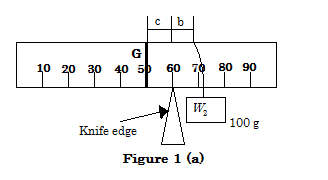
\includegraphics[width=9cm]{./img/2013-1a-alt.png}
\end{center}

\begin{enumerate}
\item[(i)] Suspend weight $W_1$ of 50 g on the left hand side of the knife edge at the position 47 cm and adjust weight $W_2$ until the metre rule balances horizontally as seen in Figure 1 (b). Read and record the lengths `a' and `b'.

\begin{center}
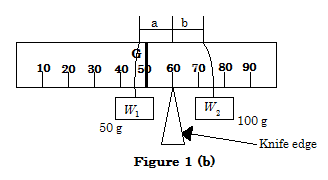
\includegraphics[width=9cm]{./img/2013-1b-alt.png}
\end{center}

\item[(ii)] Repeat the procedures in (b) (i) by adjusting the position of $W_1$ to the left at the interval of 3 cm to obtain other four (4) readings.
\end{enumerate}
\item[(c)] Tabulate your results as shown in Table 1.\\

\quad Table 1\\
\quad \quad \begin{tabular}{|p{4cm}|p{4cm}|} \hline
\multicolumn{1}{|c|}{a (cm)} & \multicolumn{1}{c|}{b (cm)} \\ \hline
& \\ \hline
& \\ \hline
\end{tabular}\\[10pt]

\item[(d)] Plot a graph of ``b'' against ``a''.
\item[(e)] What is the nature of the graph?
\item[(f)] Calculate the slope $S$ of the graph.
\item[(g)]
\begin{enumerate}
\item[(i)] Read the $b$-intercept, given that $b = Sa + \cfrac{W}{W_2} \times c$
\item[(ii)] What does $\left(\cfrac{W}{W_2}\right)c$ represent in your graph?
\item[(iii)] Calculate the value of $W$ using the relation $W_2 = \cfrac{Wc}{9.5 \text{cm}}$. What does $W$ represent?
\end{enumerate}
\item[(h)]
\begin{enumerate}
\item[(i)] Find the value of the ratio $P = \cfrac{l \times w \times t}{m}$.
\item[] \textbf{Note:} The mass $m$ of a meter rule can be obtained by calculations.
\item[(ii)] What is the physical meaning of the value of $P$?
\end{enumerate}
\item[(i)] State a possible source of error in this experiment.
\item[(j)] How can you minimize error in 1 (i)?
\item[(k)] State the aim of this experiment.
\end{enumerate}
\end{enumerate}
\flushright \textbf{(25 marks)}
\flushleft

\begin{enumerate}
\item[2.] You are provided with a Plane mirror, a Ruler, Protract, Drawing board, Optical pins, Office pins and Plain papers. Proceed as follows:
\begin{enumerate}
\item[(a)] On the plain paper provided, draw a line 13 cm from the top of the paper and call it M$_1$M$_2$. Pin your paper on the board provided and place the reflecting surface of the mirror along the line M$_1$M$_2$ as seen in Figure 2.

\begin{center}
\includegraphics[width=10cm]{./img/2013-2-alt.png}
\end{center}

\item[(b)] Insert pin O as an object at 4.0 cm in front of the mirror. Place pins P$_1$ and P$_2$ so as to appear in one straight line with the image of object O seen in the plane mirror.
\item[(c)] Remove pins P$_1$ and P$_2$, using other pins, place pins P$_3$ and P$_4$ so as to appear in a straight line with the image of object O in the other side (see Figure 2).
\item[(d)] Remove the mirror and pins. Draw lines joining P$_1$ and P$_2$ on one side and the other joining P$_3$ and P$_4$ on the other side of object O, extend both lines to meet at I on the other side of line M$_1$M$_2$.
\item[(e)] Join OI, a line cutting the reflecting surface at N.
\item[(f)] Repeat this procedure for the distance of an object being 6, 8, 10 and 12 cm.
\item[(g)] On all the diagrams drawn:
\begin{enumerate}
\item[(i)] Measure the distance ON and NI.
\item[(ii)] Comment on the distances obtained in 2 (g) (i).
\item[(iii)] What is the nature of image? Give reasons for your answer.
\item[(iv)] State four characteristics of the image you obtained.
\item[(v)] What is the aim of this experiment?
\item[(vi)] Mention and state the law governing this experiment.
\item[(vii)] Explain a source of error in this experiment.
\item[(viii)] How can you minimize the error in (vii) above?\\

\item[] \textbf{Note:} The papers used for drawing should be attached and collected together with answer booklets.
\end{enumerate}
\end{enumerate}
\end{enumerate}
\flushright \textbf{(25 marks)}
\flushleft
\vfill
\pagebreak
\index{Past Papers!Physics!2012}
\chapter{2012 - PHYSICS 2A ACTUAL PRACTICAL A}

\begin{enumerate}
\item[1.] You are provided with a measuring cylinder, eureka can, nylon thread, standard masses and water. Proceed as follows:
\begin{enumerate}
\item[(a)] Pour water into eureka can until it is just beginning to overflow.

\begin{center}
\includegraphics[width=13cm]{./img/2012-1-alt.png}
\end{center}

\item[(b)] Hold a suitable measuring cylinder under the spout and immerse a standard mass of 50 g into eureka can as shown in Figure 1. Water will pass through the spout and will be collected by the measuring cylinder. Wait for it to drop until it starts to cease and take long interval to drop. Record the reading of the water collected.
\item[(c)] Repeat the procedures in 1 (b) for standard masses of 100 g, 150 g, 200 g and 250 g.
\item[(d)] Tabulate your results showing the quantities as follows:\\

\begin{tabular}{|p{4cm}|p{4cm}|p{4cm}|}\hline
Mass (g) & Volume (cm$^3$) & Mass $\div$ Volume (g/cm$^3$) \\ \hline
50 & & \\ \hline
100 & & \\ \hline
150 & & \\ \hline
200 & & \\ \hline
250 & & \\ \hline
\end{tabular}\\[10pt]

\item[(e)] Plot a graph of mass against volume.
\item[(f)] State the nature of the graph.
\item[(g)] From the graph:
\begin{enumerate}
\item[(i)] Calculate the slope.
\item[(ii)] What does the slope of the graph show?
\item[(iii)] What is the relationship between mass and volume?
\item[(iv)] Establish the formula governing the experiment.
\end{enumerate}
\item[(h)] Identify with reasons the best to the least satisfactory method of finding the constant value of mass divide by volume.
\item[(i)] State two possible errors in this experiment.
\item[(j)] How can you minimize errors in 1 (i)?
\end{enumerate}

\pagebreak

\item[2.] You are provided with two plane mirrors, an optical pin, a sheet of plane drawing paper, mirror holder or office pins, a protractor, a ruler and a drawing table. Proceed as follows:
\begin{enumerate}
\item[(a)] Draw two lines at right angles.
\item[(b)] Place the two plane mirrors along the top two lines using the mirror holders or office pins as shown in Figure 2.

\begin{center}
\includegraphics[width=5cm]{./img/2012-2-alt.png}
\end{center}

\item[(c)] Put an optical pin at O when $\theta = 90^\circ$. Look onto one of the mirrors and count the number of images, $n$, you see.
\item[(d)] Repeat the procedures in 2 (c) for $\theta = 72^\circ$, $\theta = 60^\circ$, $\theta = 45^\circ$ and $\theta = 30^\circ$.
\item[(e)] Tabulate your results for the values of $\theta$, $n$ and $\cfrac{360^\circ}{\theta}$.
\item[(f)] Plot a graph of number of images, $n$, against $\cfrac{360^\circ}{\theta}$.
\item[(g)] From the graph:
\begin{enumerate}
\item[(i)] Determine the slope.
\item[(ii)] Find the number of images when $\cfrac{360^\circ}{\theta} = 9$
\item[(iii)] Find the value of the $y$-intercept.
\item[(iv)] Derive the equation relating the number of images and $\cfrac{360^\circ}{\theta}$
\end{enumerate}
\item[(h)] From your experiment:
\begin{enumerate}
\item[(i)] What happens to the number of images as the value angle $\theta$ is reduced?
\item[(ii)] What happens to the number of images when $\theta = 0^\circ$?
\end{enumerate}
\item[(i)] State a possible source of error and how you can minimize it.
\item[(j)] What is the aim of this experiment?
\end{enumerate}
\end{enumerate}
\vfill
\pagebreak
\index{Past Papers!Physics!2011}
\subsection{2011 - PHYSICS 2A ACTUAL PRACTICAL A}

\begin{enumerate}
\item The aim of this experiment is to determine the mass of a given dry cell size ``AA''. Proceed as follows:
\begin{itemize}
\item[(a)] Locate and note the centre of gravity $C$ of the metre rule by balancing it on the knife edge.
\item[(b)] Suspend the 50 g mass at length `$a$' cm on one side of the metre rule and the 20 g mass together with the dry cell at length `$b$' cm on the other side of the metre rule. Fix the 50 g mass at length 30 cm from the fulcrum and adjust the position of the 20 g mass together with the dry cell until the metre rule balances horizontally. Read and record the values of $a$ and $b$ as $a_0$ and $b_0$ respectively.
\item[(c)] Draw the diagram for this experiment.
\item[(d)] By fixing $a = 5$ cm from fulcrum $C$, find its corresponding length $b$.
\item[(e)] Repeat the procedure in (d) above for $a = 10$ cm, 15 cm, 20 cm and 25 cm. Tabulate your results.
\item[(f)] Draw a graph of `$a$' against `$b$' and calculate its slope $G$.
\item[(g)] Calculate $X$ from the equation $50 = \cfrac{b_0}{a_0}(20 + X)$.
\item[(h)] Comment on the value of $\cfrac{b_0}{a_0}$.
\item[(i)] Sate the principle governing this experiment.
\end{itemize}
\end{enumerate}

\flushright \textbf{(25 marks)}
\begin{enumerate}
\item[2.] You are provided with an ammeter, A, resistance box, R, dry cell, D, a key, K and connecting wires. Proceed as follows:
\begin{enumerate}
\item[(a)] Connect the circuit in series.
\item[(b)] Put $R$ = 1 $\Omega$ and quickly read the value of current $I$ on the ammeter.
\item[(c)] Repeat procedure (b) above for $R$ = 2 $\Omega$, 3 $\Omega$, 4 $\Omega$ and 5 $\Omega$. Record your results in a tabular form.
\item[(d)] Draw the circuit diagram for this experiment.
\item[(e)] Plot the graph of $R$ against $\cfrac{1}{I}$.
\item[(f)] Determine the slope of the graph.
\item[(g)] If the graph obeys the equation $R=\cfrac{E}{I}-r$, then
\begin{enumerate}
\item[(i)] suggest how $E$ and $r$ may be evaluated from your graph.
\item[(ii)] compute $E$.
\item[(iii)] compute $r$.
\end{enumerate}
\item[(h)] State one source of error and suggest one way of minimizing it.
\item[(i)] Suggest the aim of this experiment.
\end{enumerate}

\end{enumerate}

\flushright \textbf{(25 marks)}
\flushleft
\vfill
\pagebreak
\index{Past Papers!Physics!2010}
\section{2010 - PHYSICS 2A ALTERNATIVE A PRACTICAL}

\begin{enumerate}
\item[1.] The aim of this experiment is to find the mass of the unknown load labeled ``$W$'' and the spring constant $K$. Proceed as follows:

\begin{center}
\includegraphics[width=14cm]{./img/2010-1-alt.png}
\end{center}

Set up the apparatus as shown in Figure 1. Put a mass of 50 g on the scale pan and record the equilibrium position $X_0$ of the pointer. Put on the scale pan the unknown weight marked $W$. Without removing $W$ and the 50 g mass in the scale pan, add a load $L$ of 50 g and record the new position of the pointer $X$. Calculate the extension $E = (X - X_0)$. Repeat this process for $L$ = 100 g, 150 g, 200 g and 250 g.
\begin{enumerate}
\item[(a)] Record you conclusions as shown in Table 1.\\[10pt]

Equilibrium position $X_0$..................\\[10pt]

Table 1\\[10pt]

%\begin{center}
\begin{tabular}{|p{3cm}|p{3cm}|p{3cm}|} \hline
\multicolumn{1}{|c|}{Load (g)} & \multicolumn{1}{c|}{$X$ (cm)} & \multicolumn{1}{c|}{$E = X - X_0$ (cm)} \\ \hline
\multicolumn{1}{|c|}{50} & & \\ \hline
\multicolumn{1}{|c|}{100} & & \\ \hline
\multicolumn{1}{|c|}{150} & & \\ \hline
\multicolumn{1}{|c|}{200} & & \\ \hline
\multicolumn{1}{|c|}{250} & & \\ \hline
\end{tabular}\\[10pt]
%\end{center}

\item[(b)] Plot the graph of load L against absolute value of extension E. The scale of the vertical axis should be chosen to range from 200 g to 300 g.
\item[(c)] From the graph, determine the unknown weight marked W, given that L = KE + W where K is a constant.
\item[(d)] What does the gradient of the graph represent?
\item[(e)] State the sources of errors and precautions that should be taken in the experiment.
\end{enumerate}
\end{enumerate}
\flushright \textbf{(25 marks)}

\pagebreak

\begin{enumerate}
\item[2.] The aim of this experiment is to determine the refractive index of water. Proceed as follows:

\begin{center}
\includegraphics[width=10cm]{./img/2010-2-alt.png}
\end{center}

\begin{enumerate}
\item[(a)] Arrange your apparatus as in Figure 2. Put about 150 cm$^3$ of clear water in the measuring cylinder. Drop an office pin at the bottom so that it rests touching the wall of the cylinder.
\item[(b)] Look in the cylinder from Figure 2. Use another office pin as a search pin, move it up and down outside the cylinder, and locate the image position by no parallax method. Locate the image position of the ruler. Measure and record the depth ($H_1$) of the image. Measure and record the depth ($H_2$) of water. Repeat the experiment with 175 cm$^3$, 200 cm$^3$, 225 cm$^3$ and 250 cm$^3$ of water in the measuring cylinder.
\item[(c)] 
\begin{enumerate}
\item[(i)] Record in Table 2 your values of $H_1$ and $H_2$ corresponding to the volumes of water in the measuring cylinder.\\[10pt]

Table 2\\[10pt]

%\begin{center}
\begin{tabular}{|p{3cm}|p{3cm}|p{3cm}|} \hline
\multicolumn{1}{|c|}{Volume of water V (cm)} & \multicolumn{1}{c|}{$H_1$} & \multicolumn{1}{c|}{$H_2$} \\ \hline
\multicolumn{1}{|c|}{150} & & \\ \hline
\multicolumn{1}{|c|}{175} & & \\ \hline
\multicolumn{1}{|c|}{200} & & \\ \hline
\multicolumn{1}{|c|}{225} & & \\ \hline
\multicolumn{1}{|c|}{250} & & \\ \hline
\end{tabular}\\[10pt]
%\end{center}

\item[(ii)] Plot the graph of $H_2$ versus $H_1$.
\item[(iii)] Determine the slope of the graph.
\item[(iv)] What is the physical meaning of the slope?
\item[(v)] State sources of error in this experiment.
\end{enumerate}
\end{enumerate}
\end{enumerate}
\flushright \textbf{(25 marks)}

\pagebreak

\begin{enumerate}
\item[3.] The aim of this experiment is to determine the resistivity of an electrical conductor $P$.

\begin{center}
\includegraphics[width=10cm]{./img/2010-3-alt.png}
\end{center}

With $P$ having a length $l = 50$ cm, connect up the circuit as shown in Figure 3. Close one key S and adjust the rheostat R so that the current in $P$ is 0.20 A. Record the current $I$ and the potential difference $V$ between its ends.\\[10pt]

Repeat the procedure with current $I = $0.30 A, 0.40 A, 0.50 A and 0.60 A.
\begin{enumerate}
\item[(a)] Record your results in Table 3.\\[10pt]

Table 3\\[10pt]

%\begin{center}
\begin{tabular}{|p{3cm}|p{3cm}|} \hline
\multicolumn{1}{|c|}{Current $I$ (A)} & \multicolumn{1}{c|}{P.d. (volts)} \\ \hline
\multicolumn{1}{|c|}{0.20} &  \\ \hline
\multicolumn{1}{|c|}{0.30} &  \\ \hline
\multicolumn{1}{|c|}{0.40} &  \\ \hline
\multicolumn{1}{|c|}{0.50} &  \\ \hline
\multicolumn{1}{|c|}{0.60} &  \\ \hline
\end{tabular}\\[10pt]
%\end{center}

\item[(b)] Plot a graph of $V$ against $I$ and calculate the slope $G$.
\item[(c)] Deduce the resistivity of the conductor $P$ given that; $\rho = \cfrac{G\pi d^2}{4l}$.\\[10pt]
Where $\rho$ = resistivity\\
$d$ = diameter of $P$ (measured using the micrometer screw gauge provided).
\end{enumerate}
\end{enumerate}

\flushright \textbf{(25 marks)}
\flushleft
\vfill
\pagebreak
\index{Past Papers!Physics!2009}
\subsection{2009 - PHYSICS 2A ALTERNATIVE A PRACTICAL}

\begin{enumerate}
\item[1.] In this experiment you are required to find the relationship between the length of a simple pendulum and its period. Proceed as follows:
\begin{itemize}
\item[(a)] Suspend a simple pendulum of length L = 100 cm. Displace the pendulum through a small angle so that it swings parallel to the edge of the bench or table, determine the time for 20 oscillations. Continue reducing the length of the pendulum by 10 cm each time and obtain a total of six readings.
\item[(b)] Record your readings in a table as shown below.


\begin{tabular}{|p{2.5cm}|p{2.5cm}|p{2.5cm}|p{2.5cm}|p{2.5cm}|} \hline
Length of pendulum L (cm) & Log$_{10}$L & Time for 20 oscillations & Period T & Log$_{10}$T \\ \hline
&&&& \\ 
&&&& \\ 
&&&& \\ 
&&&& \\ 
&&&& \\ 
&&&& \\ 
&&&& \\ 
&&&& \\ \hline
\end{tabular}\\[10pt]

\noindent Assuming that T $ \propto $ L$^a$, we have T = $k$L$^a$ and taking logarithms to base ten on both sides we get $\log_{10}$T = $a\log_{10}$L + $\log_{10}k$.

\begin{itemize}
\item[(i)] Plot a graph of $\log_{10}$T (vertical axis) against $\log_{10}$L (horizontal axis) hence determine the values of $a$ and $k$ each correct to one decimal place.
\item[(ii)] From your answer in (i) above write down the values of $a$ and $k$ each in the form of $\cfrac{b}{c}$ where $b$ and $c$ are integers (i.e. whole numbers).
\item[(iii)] From the assumption and your answer in (ii) deduce the form of the equation governing the motion of the simple pendulum.
\end{itemize}

\end{itemize}
\end{enumerate}
\flushright \textbf{(25 marks)}


\begin{enumerate}
\item[2.] The aim of this experiment is to determine the refractive index $\eta$ of a given glass block.

\begin{center}
\includegraphics[width=8cm]{./img/2009-2-alt.png}
\end{center}

Place the rectangular glass block on the white paper on a drawing board. Using a pencil trace the outline of the block. Remove the glass block and draw a normal NOM near the left end of the block (Figure 1).\\[10pt]

\noindent Using a protractor and a pencil measure $\theta = 20^\circ$, draw a line making the angle $20^\circ$ with the surface RR of the block. Erect two pins T$_1$ and T$_2$ on this line and at a suitable distance from one another. Return the block and erect the pins T$_3$ and T$_4$ at positions such that they lie in a straight line with pins T$_1$ and T$_2$ as seen through the block. Now remove the block and draw a complete path of the ray (Figure 1).\\[10pt]

\noindent Measure the length MN$'$ and ON$'$: Repeat the procedure for values of $\theta = 30^\circ, 40^\circ$ and $60^\circ$ respectively. In each case make a drawing on a fresh part of the drawing paper.

\begin{itemize}
\item[(a)] Record the values of $\theta$, MN$'$, ON$'$, $\cfrac{\text{MN}'}{\text{ON}'}$ and $\cos \theta$ in a tabular form.
\item[(b)] Plot a graph of $\cfrac{\text{MN}'}{\text{ON}'}$ against $\cos \theta$.
\item[(c)] Find the slope $G$ of the graph.
\item[(d)] Calculate the value of the refractive index $\eta$; given that $G = \cfrac{1}{\eta}$.
\item[(e)] State two sources of errors. \hfill \textbf{(25 marks)}
\end{itemize}

\end{enumerate}


\begin{enumerate}
\item[3.] The aim of this experiment is to verify Ohm's Law.

\begin{center}
\includegraphics[width=7cm]{./img/2009-3-alt.png}
\end{center}

\begin{itemize}
\item[(a)] Set up the apparatus as shown on Figure 2, close switch S. Adjust the Rheostat Rh by sliding slowly from one end, read and record the value V of the voltmeter and current I of the ammeter.
\item[(b)] Repeat the experiment by changing the Rheostat slider to obtain about five pair of readings.\\[10pt]

\textbf{NB:} Adjust the Rheostat until when the pointer is exactly on the division of the metre scale.\\[10pt]

Table of results\\[10pt]
\begin{tabular}{|c|c|c|c|c|c|c|c|}\hline
V (V)&&&&&&&\\ \hline
I (A)&&&&&&& \\ \hline
\end{tabular}

\item[(c)] Plot a graph of V (vertical axis) against I (horizontal axis).
\item[(d)] 
\begin{itemize}
\item[(i)] Find the slope of the graph.
\item[(ii)] What is the relation between V and I?
\item[(iii)] Find the resistance R. \hfill \textbf{(25 marks)}
\end{itemize}
\end{itemize}

\end{enumerate}
\flushleft

\vfill
\pagebreak
\index{Past Papers!Physics!2008}
\section{2008 - PHYSICS 2A  ALTERNATIVE A PRACTICAL}

\begin{enumerate}
\item[1.] The aim of this experiment is to investigate whether string A obeys Hooke's law.

\begin{center}
\includegraphics[width=15cm]{./img/2008-1-alt.png}
\end{center}

Proceed as follows:\\[6pt]

Clamp string A at one end, attach a weighing pan at the other end and a pointer to give a reading on a scale as shown in figure 1 above.\\[6pt]

Measure the height, $h_0$ when the pan is empty.\\[6pt]

Place 50 g mass on the pan and record the new height $h$ indicated by the pointer.\\[6pt]

Add another 50 g mass each time up to 300 g, and record the corresponding values of $h$ for added mass.

\begin{enumerate}
\item[(a)] Tabulate your results as shown in the table below.
\item[] $h_0 = $ \begin{tabular}{p{1.5cm}}
\\ \hline
\end{tabular} cm.\\[10pt]

\begin{tabular}{|c|c|c|c|c} \hline
Mass, $m$ (g) & Height, $h$ (cm) & Extension ($h - h_0$) & Stretching \\
&&(cm)&force, $F$ (N) \\ \hline
50&&& \\ 
100&&& \\ 
150&&& \\ 
200&&& \\ 
250&&& \\ 
300&&& \\ \hline
\end{tabular}\\[10pt]
\item[(b)] Plot a graph of force $F$ (N) against extension (cm).
\item[(c)] From the graph find the
\begin{enumerate}
\item[(i)] slope, K of the graph.
\item[(ii)] extension caused by a mass of 180 g.
\end{enumerate}
\item[(d)] Deduce whether string A obeys Hooke's law.
\item[(e)] State the law. \hfill \textbf{(25 marks)}
\end{enumerate}
\end{enumerate}

\begin{enumerate}
\item[2.] You are provided with a glass block, four sheets of drawing paper, four optical pins (or office pins) and a drawing board.\\[6pt]

Proceed as follows:\\[6pt]

Place the glass block flat on the drawing paper fixed to the drawing board and with a sharp pencil, draw its outline.

\begin{center}
\includegraphics[width=9cm]{./img/2008-2-alt.png}
\end{center}

Remove the glass block and draw a normal NN' to the longer edge of the block (see fig. 2).\\
Draw a line making an angle of incidence ($i$) of 30$^\circ$. Stick two vertical pins P$_1$ and P$_2$ on this line. Replace the glass block. Stick two more pins P$_3$ and P$_4$ on the other side of the block so that they appear to be in the same straight line with the images of pins P$_1$ and P$_2$ as seen through the block.\\
Remove the block and draw the complete path of the ray entering and leaving the block.\\
Measure the angle of refraction ($r$).\\[6pt]

Produce the incident ray as shown in fig. 2 and measure the perpendicular distance ($d$) between the incident ray and the emergent ray.\\
Repeat this procedure for angles of incidence of $40^\circ$, $50^\circ$, $60^\circ$ and $70^\circ$. In each case draw the block again on a fresh part of the paper.
\begin{enumerate}
\item[(a)] Record your results in a table as follows:
\begin{tabular}{|p{0.15\textwidth}|p{0.15\textwidth}|p{0.15\textwidth}|p{0.15\textwidth}|p{0.15\textwidth}|} \hline
\multicolumn{1}{|c|}{$i^\circ$} & \multicolumn{1}{c|}{$r^\circ$} & \multicolumn{1}{c|}{$d$ (cm)} & \multicolumn{1}{c|}{$d\cos{r}$ (cm)} & \multicolumn{1}{c|}{$\sin{(i-r)}$} \\ \hline
\multicolumn{1}{|c|}{30}&&&& \\
\multicolumn{1}{|c|}{40}&&&& \\
\multicolumn{1}{|c|}{50}&&&& \\
\multicolumn{1}{|c|}{60}&&&& \\
\multicolumn{1}{|c|}{70}&&&& \\ \hline
\end{tabular}\\[10pt]
\item[(b)] Plot a graph of $d \cos{r}$ (vertical axis) against $\sin{(i - r)}$ (horizontal axis).
\item[(c)] Find the gradient of the graph.
\item[(d)] Measure the width of the glass block.
\item[(e)] How is the gradient related to the with of the glass block?
\item[] NB: Hand in your diagrams together with your answer booklet. \hfill \textbf{(25 marks)}
\end{enumerate}
\end{enumerate}

\begin{enumerate}
\item[3.] The aim of this experiment is to determine the resistance of a wire W.\\
Proceed as follows:
\begin{enumerate}
\item[(a)] Connect in series the full length of wire W of unknown resistance, battery B (3 V), a switch K, a rheostat Rh of a few ohms and an ammeter A of $0 - 1$ A.\\
Connect the voltmeter V of $0 - 3$ V across W. Check that the +ve side of the ammeter A and the +ve side of the voltmeter V are both on the +ve side of the battery B.
\item[(b)] Switch on the current. Adjust the rheostat to obtain five widely different values of $V$ and corresponding values of current $I$.
\item[(c)] Tabulate your results as follows:\\[10pt]
\begin{tabular}{|p{4cm}|p{4cm}|} \hline
\multicolumn{1}{|c|}{Potential difference} & \multicolumn{1}{c|}{Current $I$ (amperes)} \\
\multicolumn{1}{|c|}{$V$ (volts)} & \\ \hline
& \\ 
& \\ 
& \\ \hline
\end{tabular}
\item[(d)]
\begin{enumerate}
\item[(i)] Draw a circuit diagram.
\item[(ii)] Plot a graph of potential difference $V$ against current $I$.
\item[(iii)] Find the slope of the graph.
\item[(iv)] Determine the resistance of the wire W.
\item[(v)] Mention \textbf{two (2)} main precautions to be taken in this experiment.
\end{enumerate}
\end{enumerate}
\end{enumerate}
\flushright \textbf{(25 marks)}
\flushleft
\vfill
\pagebreak
\index{Past Papers!Physics!2007}
\section{2007 - PHYSICS 2A ALTERNATIVE A PRACTICAL}

\begin{enumerate}
\item[1.] The aim of this experiment is to determine the mass of a given object ``B'', and the constant of the spring provided.

\begin{center}
\includegraphics[width=7cm]{./img/2007-1-alt.png}
\end{center}

\begin{itemize}
\item[]
\begin{itemize}
\item[(i)] Set up the apparatus as shown in Fig. 1 with zero mark of the metre-rule at the top of the rule and record the scale reading by the pointer, $S_0$.
\item[(ii)] Place the object ``B'' and standard weight (mass) W equal to 20 g in the pan and record the new pointer reading $S_1$. Calculate the extension, $e = S_1 - S_0$ in cm.
\item[(iii)] Repeat the procedure in (ii) above with W = 40 g, 60 g, 80 g and 100 g.
\end{itemize}
\item[(a)] Record your results in tabular form as shown below:\\
Table of Results:

\begin{tabular}{|p{2cm}|p{3cm}|p{3cm}|p{3cm}|}\cline{1-1}
\multicolumn{1}{|p{2cm}|}{$S_0 = $}&\multicolumn{2}{c}{} & \multicolumn{1}{p{2.5cm}}{} \\ \hline
\multicolumn{1}{|c|}{Mass} & \multicolumn{1}{c|}{Force, F (N)} & \multicolumn{1}{c|}{Pointer reading $S_1$} & \multicolumn{1}{c|}{Extension}\\
\multicolumn{1}{|c|}{(kg)} & \multicolumn{1}{c|}{} & \multicolumn{1}{c|}{(cm)} & \multicolumn{1}{c|}{$= S_1 - S_0$ (cm)}\\ \hline
\multicolumn{1}{|c|}{0} & \multicolumn{1}{c|}{} & \multicolumn{1}{c|}{} & \multicolumn{1}{c|}{}\\ 
\multicolumn{1}{|c|}{0.02} & \multicolumn{1}{c|}{} & \multicolumn{1}{c|}{} & \multicolumn{1}{c|}{}\\ 
\multicolumn{1}{|c|}{0.04} & \multicolumn{1}{c|}{} & \multicolumn{1}{c|}{} & \multicolumn{1}{c|}{}\\ 
\multicolumn{1}{|c|}{0.06} & \multicolumn{1}{c|}{} & \multicolumn{1}{c|}{} & \multicolumn{1}{c|}{}\\ 
\multicolumn{1}{|c|}{0.08} & \multicolumn{1}{c|}{} & \multicolumn{1}{c|}{} & \multicolumn{1}{c|}{}\\ 
\multicolumn{1}{|c|}{0.10} & \multicolumn{1}{c|}{} & \multicolumn{1}{c|}{} & \multicolumn{1}{c|}{}\\ \hline
\end{tabular}
\item[(b)] Plot graph of Force F (vertical axis) against extension $e$ (horizontal axis).
\item[(c)] Use your graph to evaluate
\begin{itemize}
\item[(i)] mass of B
\item[(ii)] spring constant, K, given that force, extension, constant and weight of B are related as follows:\\
F = K$e$ - B
\end{itemize}
\end{itemize}

\end{enumerate}
\flushright \textbf{(25 marks)}



\begin{enumerate}
\item[2.] The aim of this experiment is to find the refractive index of a glass block. Proceed as following:\\[10pt]

Place the given glass block in the middle of the drawing paper on the drawing board. Draw lines along the upper and lower edge of the glass block. Remove the glass block and extend the line you have drawn. Represent the ends of those line segments as SS$^1$ and TT$^1$. Draw the normal NN$^1$ to the parallel lines SS$^1$ and TT$^1$ as shown in Fig. 2(a).

\begin{center}
\includegraphics[width=8cm]{./img/2007-2a-alt.png}
\end{center}

Draw five evenly spaced lines from O to represent incident rays at different angles of incidence (10$^\circ$, 20$^\circ$, 30$^\circ$, 40$^\circ$ and 50$^\circ$ from the normal). Replace the glass block carefully between SS$^1$ and TT$^1$. Stick two pins P$_1$ and P$_2$ as shown in Fig. 2(b) as far apart as possible along one of the lines drawn to represent an incident ray. Locate an emergent ray by looking through the block and stick pins P$_3$ and P$_4$ exactly in line with images I$_1$ and I$_2$ of pins P$_1$ and P$_2$. Draw the emergent ray and repeat the procedure for all the incident rays you have drawn. Finally draw in the corresponding refracted rays.\\[10pt]

NOTE: The drawing paper should be handed in together with other answer sheets.

\begin{center}
\includegraphics[width=10cm]{./img/2007-2b-alt.png}
\end{center}

\begin{itemize}
\item[(a)] Record the angles of incidence I and the measured corresponding angles of refraction ``r'' in a table. Your table of results should include the values of $\sin$ I and $\sin$ r.
\item[(b)] Plot the graph of $\sin$ I (vertical - axis) against $\sin$ r (horizontal - axis).
\item[(c)] Determine the slope of the graph.
\item[(d)] What is the refractive index of the glass block used?
\item[(e)] Mention any sources of errors in this experiment.
\end{itemize}

\end{enumerate}
\flushright \textbf{(25 marks)}


\begin{enumerate}
\item[3.] The aim of this experiment is to determine the potential fall along a uniform resistance wire carrying a steady current.\\[10pt]

Proceed as follows:

\begin{center}
\includegraphics[width=12cm]{./img/2007-3-alt.png}
\end{center}

Connect up the circuit as shown in Fig. 3. Adjust the rheostat so that when the sliding contact J is near B, and the key is closed the voltmeter V indicates an almost full scale deflection. Do not alter the rheostat again.\\

Close key K and make contact with J, so that AJ = 10 cm. Record the potential different V volts between A and J as registered on the voltmeter.\\

Repeat this procedure for AJ = 20 cm, 30 cm, 50 cm and 70 cm.

\begin{itemize}
\item[(a)] Tabulate your results for the values of AJ and V.
\item[(b)] Plot a graph of V (vertical axis) against AJ (horizontal axis).
\item[(c)] Calculate the slope of the graph.
\item[(d)] What is your comment on the slope?
\item[(e)] State any precautions on the experiment.
\end{itemize}

\end{enumerate}
\flushright \textbf{(25 marks)}
\flushleft
\vfill
\pagebreak
\index{Past Papers!Physics!2006}
\section{2006 - PHYSICS 2A ALTERNATIVE A PRACTICAL}

\begin{enumerate}
\item[1.] In this experiment you are required to determine the mass of unknown object ``X''.

\begin{center}
\includegraphics[width=10cm]{./img/2006-1-alt.png}
\end{center}

Assemble the pieces of apparatus as shown in Figure 1, with zero mark scale of the rule at the lower most end.\\

Record the reading of the position of pointer on the scale of metre-rule when the pan is empty as $S_0$.\\

Put 20 g to the pan and record pointer reading $S$.\\

Find extension $e = S - S_0$ cm.\\

Repeat the procedure for mass of 40 g, 60 g, 80 g and 100 g. Put object X on the pan and record its pointer reading.

\begin{itemize}
\item[(a)] Summarize your results in a table as follows:\\[10pt]
\begin{center}
\begin{tabular}{|l|c|c|c|c|c|c|} \hline
Mass on pan (g) &20&40&60&80&100&X \\ \hline
Pointer reading (cm) &&&&&& \\ \hline
Extension, $e = S - S_0$ (cm) &&&&&& \\ \hline
\end{tabular} \\[10pt]
\end{center}
\item[(b)] Plot graph of mas against extension (m Vs. $e$).
\item[(c)] Find slope, P, of your graph.
\item[(d)] Find mass X.
\item[(e)] Find Q, given that Q = P $\times$ $e_\text{x}$, where $e_\text{x}$ is extension of X.
\item[(f)] Comment on Q and X.
\end{itemize}


\end{enumerate}

\begin{enumerate}
\item[2.] Set up the experiment as shown in the diagram below using plane mirror, soft board, three pins and a white sheet of paper.

\begin{center}
\includegraphics[width=6cm]{./img/2006-2-alt.png}
\end{center}

Fix a white sheet of paper on the soft board. Draw a line across the width at about the middle of the white sheep (MP). Draw line ONI perpendicular to MP.\\

Fix optical pin O to make ON = U = 3 cm. By using plasticine or otherwise, fix plane mirror along portion of MP with O in front of the mirror. With convenient position of eye, E, look into the mirror and fix optical pins A and B to be in line with image, I, of pin O.\\

Measure and record NI = V. Repeat procedure for U = 6 cm, 9 cm and 12 cm.

\begin{itemize}
\item[(a)] Tabulate your results as follows:\\[10pt]

\quad \quad \begin{tabular}{|l|c|c|c|c|} \hline
U (cm) &3&6&9&12 \\ \hline
V (cm) &&&& \\ \hline
\end{tabular} \\[10pt]

\item[(b)] Plot graph of U against V.
\item[(c)] Calculate slope, m, of the graph to the nearest whole number.
\item[(d)] State relationship between U and V.
\item[(e)] Write equation connecting U and V using numerical value of m with symbols U and V.
\item[(f)] From your equation give position of the image when object is touching the face of the mirror.
\end{itemize}

\end{enumerate}


\begin{enumerate}
\item[3.] You are required to determine the unknown resistance labeled X using a metre bridge circuit. Connect your circuit as shown below, where R is a resistance box, G is a galvanometer, J is a jockey and others are common circuit components.

\begin{center}
\includegraphics[width=14cm]{./img/2006-3-alt.png}
\end{center}

Procedure:\\

With R = 1 $\Omega$, obtain a balance point on a metre bridge wire AB using a jockey J. Note the length $l$ in centimetres. Repeat the experiment with R equal to 2 $\Omega$, 4 $\Omega$, 7 $\Omega$ and 10 $\Omega$.\\

Tabulate your results for R, $l$ and $^1/_l$.

\begin{itemize}
\item[(a)]
\begin{itemize}
\item[(i)] Plot a graph of R (vertical axis) against $^1/_l$ (horizontal axis).
\item[(ii)] Determine the slope S of your graph.
\item[(iii)] Using your graph, find the value of R for which $^1/_l = 0.02$.
\end{itemize}
\item[(b)] Read and record the intercept R$_0$ on the vertical axis.
\item[(c)] Given that,\\
\quad \quad R = $\cfrac{100\text{X}}{l}$ - X\\
Use the equation and your graph to determine the value of X.
\item[(d)] Comment on your results in (a)(iii), (b) and (c) above.
\end{itemize}

\end{enumerate}
\vfill
\pagebreak
\index{Past Papers!Physics!2005}
\subsection{2005 - PHYSICS 2A ALTERNATIVE A PRACTICAL}

\begin{enumerate}
\item[1.] The aim of this experiment is to determine the mass of unknown weight labelled \textbf{X} and the force constant of the spring \textbf{k}.

\begin{center}
\includegraphics[width=12cm]{./img/2005-1-alt.png}
\end{center}

Set up the apparatus provided as shown in figure 1 above. Add 50 g mass on to the weight pan so that any ``kinks'' in the spring are removed. Leave this weight for the whole experiment but ignore it in all readings. Record the scale reading $S_0$. Add 50 g on to the weight pan and record the new scale reading $S$. Calculate the extension ($e = S - S_0$) caused by the weight. Repeat with different weights ($W$) to obtain at least five readings. Tabulate your results. Replace the weights ($W$) by the weight \textbf{X} provided and find the corresponding extension.\\[10pt]

Record this extension as $S_{\text{X}}$ ............. cm

\begin{enumerate}
\item[(a)] Plot a graph of load against extension.
\item[(b)]
\begin{enumerate}
\item[(i)] Find the gradient (G) of your graph.
\item[(ii)] What is the physical meaning of the gradient?
\end{enumerate}
\item[(c)] From the graph, what is the mass of the weight labelled \textbf{X}?
\end{enumerate}

\item[2.] The aim of this experiment is to find the critical angle \textbf{C} of the given glass block.

\begin{center}
\includegraphics[width=10cm]{./img/2005-2-alt.png}
\end{center}

\textbf{Proceed as follows:}\\[10pt]

Place a white sheet of paper on the drawing board. Place the glass block, with one of its largest surfaces top most on top of the white paper. Mark the outline of the glass block on the paper with a pencil. Then remove the glass block and draw a line which cuts its largest sides normally at E and F as shown in figure 2 above. \\[10pt]

Using a protractor draw an angle $\alpha = 30^\circ$ with the glass block. Replace the glass block in its original position and stick the first pin P$_1$ and second pin P$_2$ along the line of angle $\alpha = 30^\circ$. Stick the third and fourth pins P$_3$ and P$_4$ respectively on the opposite side of the glass block such that P$_3$ and P$_4$ fall on a straight line with P$_1$ and P$_2$ when viewed through side CD of the glass block. \\[10pt]

Remove the glass block and trace the straight path taken by the ray G P$_3$ P$_4$. Using a ruler, join G and E. \\[10pt]

Measure the angle of refraction $r^\circ$, then calculate the values of $\cos{\alpha}$ and $\sin{r^\circ}$. Repeat the same procedure for values $\alpha = 40^\circ$, $50^\circ$, $60^\circ$, $70^\circ$ and $80^\circ$. Record your results in tabular form for the values of $\alpha$, $r^\circ$, $\sin{r^\circ}$ and $\cos{\alpha}$.

\begin{enumerate}
\item[(a)] Plot a graph of $\sin{r^\circ}$ (vertical axis) against $\cos{\alpha}$ (horizontal axis).
\item[(b)] Find the slope of the graph.
\item[(c)] Calculate the value of $C$ where slope = $\sin{C}$.
\item[(d)] State the possible sources of error and precautions you have taken during the experiment.
\end{enumerate}

\item[3.] The aim of this experiment is to determine the \textbf{e.m.f. E} and internal resistance \textbf{r} of a cell.

\begin{center}
\includegraphics[width=7cm]{./img/2005-3-alt.png}
\end{center}

\begin{enumerate}
\item[(a)] Connect the circuit as shown in figure 3 above. Put $R = 1 \Omega$ and quickly read the value of $i$ on the ammeter.
\item[(b)] Repeat the procedure in 3 (a) above, for values of $R = 2 \Omega$, $3 \Omega$, $4 \Omega$ and $5 \Omega$ respectively.
\item[(c)] Tabulate your results and complete the following table.
\begin{center}
\begin{tabular}{|c|c|c|} \hline
\textbf{Resistance $R$ ($\Omega$)} & \textbf{Current $i$ (A)} & \textbf{$\cfrac{1}{i} \left(\text{A}^{-1}\right)$ } \\ \hline
1&& \\
2&& \\
3&& \\
4&& \\
5&& \\ \hline
\end{tabular} \\[10pt]
\end{center}
\item[(d)] Plot the graph of $R$ against $\cfrac{1}{i}$.
\item[(e)] The graph uses the equation $R = \cfrac{E}{i} - r$.
\begin{enumerate}
\item[(i)] Suggest how $E$ and $r$ may be evaluated from your graph.
\item[(ii)] Evaluate $E$ for one cell.
\item[(iii)] Evaluate $r$ for one cell.
\end{enumerate}
\item[(f)] State one source of error and suggest one way of minimizing it.
\end{enumerate}

\end{enumerate}
\vfill
\pagebreak
\index{Past Papers!Physics!2004}
\subsection{2004 - PHYSICS 2A ALTERNATIVE A PRACTICAL}

\begin{enumerate}
\item[1.] The aim of this experiment is to determine the mass of a given dry cell, size ``AA''.\\[5pt]

You are provided with a dry cell, a knife edge, two weights 50 g and 20 g, and a metre rule.\\[5pt]

Proceed as follows:
\begin{enumerate}
\item[(a)] Locate and note the centre of gravity C of the metre rule by balancing on the knife edge.
\item[(b)] Suspend the 50 g mass on one side of the metre rule, and 20 g together with the dry cell on the other side of the metre rule adjusting their position until the metre rule balances horizontally, as shown in Figure 1 below.

\begin{center}
\includegraphics[width=10cm]{./img/2004-1-alt.png}
\end{center}

\item[(c)] By fixing a = 5 cm from C find its corresponding length, b, from C.
\item[(d)] Repeat and tabulate your results using a = 10 cm, 15 cm, 20 cm and 25 cm.
\item[(e)] Draw a graph of ``a'' against ``b'' and calculate its slope G.
\item[(f)] Calculate X from the equation $\text{G} = \cfrac{20 + \text{X}}{50}$. \hfill \textbf{(25 marks)}
\end{enumerate}


\item[2.] You are provided with a glass block, drawing board, optical pins and plane papers.\\

Place a white piece of paper on the drawing board. Place the glass block with one of its largest surface top most on top of the white paper. Mark the outline of the glass block on the paper with a pencil. Remove the glass block and draw a normal as shown in Figure 2 below.

\begin{center}
\includegraphics[width=10cm]{./img/2004-2-alt.png}
\end{center}

\begin{enumerate}
\item[(a)] Draw a line making an angle of incidence, $i$ of $30^\circ$. Erect two pins P$_1$ and P$_2$ on this line at a suitable distance apart. Replace the glass block and erect two more pins P$_3$ and P$_4$ at positions which appear to be in a straight line with the other two pins as seen through the glass block from the other side.\\[10pt]

Remove the glass block and draw the complete path of the ray (see Fig. 2). Measure the angle of refraction, $r$.
\item[(b)]
\begin{enumerate}
\item[(i)] Extend the direction of the incident ray as shown by the dotted line.
\item[(ii)] Measure the perpendicular distance `$d$' between extended incident ray and the emergent ray.
\end{enumerate}
\item[(c)] Repeat the procedure in (a) and (b) above for angles of incidence of $30^\circ$, $40^\circ$, $50^\circ$, $60^\circ$ and $70^\circ$. (In each case make your drawings on a fresh part of the drawing paper).
\item[(d)] Tabulate your results as shown in Table 1 below.
\begin{center}
\begin{tabular}{|p{0.15\textwidth}|p{0.15\textwidth}|p{0.15\textwidth}|p{0.15\textwidth}|p{0.15\textwidth}|} \hline
\multicolumn{1}{|c|}{$i$ (deg)} & \multicolumn{1}{c|}{$r$ (deg)} & \multicolumn{1}{c|}{$d$ (cm)} & \multicolumn{1}{c|}{$d\cos{r}$} & \multicolumn{1}{c|}{$\sin{(i-r)}$} \\ \hline
\multicolumn{1}{|c|}{30}&&&& \\
\multicolumn{1}{|c|}{40}&&&& \\
\multicolumn{1}{|c|}{50}&&&& \\
\multicolumn{1}{|c|}{60}&&&& \\
\multicolumn{1}{|c|}{70}&&&& \\ \hline
\end{tabular}\\[10pt]
\end{center}
\begin{enumerate}
\item[(i)] Plot a graph of $d\cos{r}$ against $\sin{(i-r)}$.
\item[(ii)] Find the gradient of the graph.
\item[(iii)] Measure the width of the glass block.
\item[(iv)] How is the gradient of the graph in 2 (a)(ii) and the width of the glass block in 2 (a)(iii) related?\\[5pt]
\end{enumerate}
\item[] NB: \quad Hand in your diagrams (drawings) together with your answer booklet. 
\item[] \flushright \textbf{(25 marks)}

\end{enumerate}

\item[3.] Determine the resistivity $\rho$ of the wire labelled W and the internal resistance of the battery provided.\\

Proceed as follows:

\begin{center}
\includegraphics[width=10cm]{./img/2004-3-alt.png}
\end{center}

Connect the circuit as shown in fig. 3 above. With the plug key open adjust the length of wire W to a value of 20 cm. Note the ammeter reading.\\[10pt]

\noindent NB: The plug key should remain open throughout the experiment.

\begin{enumerate}
\item[(a)] Repeat the procedure above for $L_W$ = 40 cm, 60 cm, 80 cm and 100 cm each time recording the ammeter reading.
\item[(b)] Tabulate your results as shown in Table 2 below.

\begin{tabular}{|p{2.5cm}|c|c|} \hline
Length $L_W$ of wire (cm)& Current $I$ (A)& $\cfrac{1}{I} \left(\text{A}^{-1}\right)$ \\ \hline
&& \\
&& \\
&& \\
&& \\ \hline
\end{tabular}\\[10pt]

\item[(c)]
\begin{enumerate}
\item[(i)] Plot a graph of $\cfrac{1}{I}$ (vertical) against $L_W$ (horizontal).
\item[(ii)] Determine the slope G.
\item[(iii)] Determine the intercept $Y$ on the vertical axis.
\end{enumerate}
\item[(d)] Measure and record the diameter at four different places on the wire. Hence find the mean value of diameter $d$.
\item[(e)] Given that $G = \cfrac{4\rho}{\pi d^2E}$ and $Y = \cfrac{R + r}{E}$\\[10pt]
Where $E$ is the emf of the battery, and $R = 2 \Omega$, Find the
\begin{enumerate}
\item[(i)] Resistivity $\rho$ of the wire.
\item[(ii)]	Internal resistance $r$ of the battery. \hfill \textbf{(25 marks)}
\end{enumerate}
\end{enumerate}

\end{enumerate}
\vfill
\pagebreak
\setcounter{secnumdepth}{2}




% Headers and footers ("Page Styles" chapter in LaTeX manual)
\setlength{\headheight}{15pt}

\pagestyle{fancy}
\renewcommand{\chaptermark}[1]{ \markboth{#1}{} }
\renewcommand{\sectionmark}[1]{ \markright{#1}{} }

\fancyhf{}
\fancyhead[LE,RO]{\thepage}
\fancyhead[RE]{\textit{ \nouppercase{\leftmark}} } % \leftmark shows Chapter Name
\fancyhead[LO]{\textit{ \nouppercase{\leftmark}} } % \rightmark shows Section Name

\fancypagestyle{plain}{ % specific for plain pages (chapter pgs)
	\fancyhf{} % remove everything
	\fancyhf[FC]{\thepage} % show the page number
	\renewcommand{\headrulewidth}{0pt} % remove lines as well
	\renewcommand{\footrulewidth}{0pt}
}


% Other appendix chapters
\settocdepth{chapter} % Keep the ToC nice and tidy for these appendices.
\chapter{Sources of Laboratory Equipment} \index{Equipment! sources of}
\label{cha:labequip}
In order to gain a thorough understanding of science, students must be able to make a connection between classroom learning and the outside world. The following is a list of locally available materials which may be used to substitute conventional materials and apparatus for various activities. These materials have the following advantages: 
\begin{itemize*}
\item They are readily available in the village or a nearby town;
\item They are cheaper than conventional materials; 
\item They may safely substitute the conventional materials without fear of losing accuracy or understanding; 
\item They help students to draw a connection between science education and the world around them.
\end{itemize*}
Imagination and innovativeness is encouraged on the part of the student and teacher to find other suitable local substitutions. 

How many experiments can be carried out with everyday items?

\begin{center}
\includegraphics[width=12cm]{./img/vso/using-local-materials.jpg}
\includegraphics[width=12cm]{./img/vso/multi-purpose-bottle.jpg}
\end{center}

Below are common apparatus you might order from a laboratory supply company, 
and comments about which have good if not superior alternatives 
available in villages and towns. 
Given equal quality, 
it is generally better to use local materials, 
because these help connect classroom learning to students' lives.\\

The apparatus listed in this section are the following:

\begin{multicols}{3}

\begin{enumerate}
\item \nameref{sec:alligator-clips}
\item \nameref{sec:balance}
\item \nameref{sec:beakers}
\item \nameref{sec:blowpipe}
\item \nameref{sec:lightbulbs}
\item \nameref{sec:bunsen-burner}
\item \nameref{sec:burettes}
\item \nameref{sec:circuit-comp}
\item \nameref{sec:crucible}
%\item \nameref{sec:condenser}
\item \nameref{sec:containers}
\item \nameref{sec:deflagratingspoon}
\item \nameref{sec:delivery-tube}
\item \nameref{sec:drawing-board}
\item \nameref{sec:droppers}
\item \nameref{sec:electrodes}
\item \nameref{sec:electrode-holder}
%\item \nameref{sec:electrolytic-cell}
\item \nameref{sec:eureka-can}
\item \nameref{sec:filter-paper}
\item \nameref{sec:flasks}
\item \nameref{sec:funnel}
\item \nameref{sec:glass-blocks}
\item \nameref{sec:gloves}
\item \nameref{sec:goggles}
\item \nameref{sec:heatsources}
\item \nameref{sec:indicator}
\item \nameref{sec:iron-filings}
\item \nameref{sec:masses}
\item \nameref{sec:meascyl}
\item \nameref{sec:meter-rule}
\item \nameref{sec:microscope}
\item \nameref{sec:mirrors}
\item \nameref{sec:mortar-and-pestle}
\item \nameref{sec:nichrome-wire}
\item \nameref{sec:optical-pins}
\item \nameref{sec:pipettes}
\item \nameref{sec:pulleys}
\item \nameref{sec:resistors}
\item \nameref{sec:retort-stand}
\item \nameref{sec:scale-pan}
\item \nameref{sec:scalpels}
\item \nameref{sec:slide-cover-slip}
\item \nameref{sec:spatula}
\item \nameref{sec:spring-balance}
\item \nameref{sec:springs}
\item \nameref{sec:stoppers}
\item \nameref{sec:stopwatches}
\item \nameref{sec:testtubes}
\item \nameref{sec:test-tube-brush}
\item \nameref{sec:test-tube-holder}
\item \nameref{sec:test-tube-racks}
\item \nameref{sec:tripod-stands}
\item \nameref{sec:volumetric-glassware}
\item \nameref{sec:wash-bottle}
\item \nameref{sec:hotwaterbathes}
\item \nameref{sec:weights}
\item \nameref{sec:white-tiles}
\item \nameref{sec:wire}
\item \nameref{sec:wire-gauze}
\end{enumerate}

\end{multicols}

\begin{multicols}{2}

\section{Alligator Clips} \index{Alligator clips}
\label{sec:alligator-clips}
\vspace{-10pt}
\textbf{Use:} Connecting electrical components\\
\textbf{Materials:} Clothespins, aluminum foil, glue\\
\textbf{Procedure:} Glue aluminum foil around the clamping tips of a clothespin.

\section{Balance} \index{Beam balance! construction of}
\label{sec:balance}
\vspace{-10pt}
\textbf{Use:} Measuring mass\\
\textbf{Materials:} Ruler or wooden bar 30 cm $\times$ 2 cm, nails, razor/knife, string/wire, pen, 2 \nameref{sec:scale-pan}\\
\textbf{Procedure:} Find the balancing point of the ruler/wood block and mark it with a pen. Use a heated nail to make a hole through this point. Make notches at 5 cm intervals on either side of the center hole using a razor/knife to suspend scale pans. Use a string/wire tied through the center hole to suspend the balance.
\begin{center}
\includegraphics[width=0.45\textwidth]{./img/beam-balance.png}
\end{center}

\section{Beakers} \index{Beakers}
\label{sec:beakers}
\vspace{-10pt}
\textbf{Use:} To hold liquids, to heat liquids\\
\textbf{Materials:} Water bottles, jam jars, metal cans, knife\slash razor\\
\textbf{Procedure:} Take empty plastic bottles of different sizes. Cut them in half. The base can be used as a beaker. Jam jars made of glass, cut off metal cans and aluminum pots may be used when heating.\\
\textbf{Safety:} Glass containers may shatter if heated too much. Use standard laboratory equipment if extreme heating is needed.
\begin{center}
\includegraphics[width=8cm]{./img/vso/beakers.jpg}
\end{center} 

\section{Blowpipe} \index{Blowpipe}
\label{sec:blowpipe}
\vspace{-10pt}
\textbf{Use:} Increasing temperature of flames\\
\textbf{Materials:} Syringe needle, tube/straw/pen tube\\
\textbf{Procedure:} For sterilisation heat the needle
in open fire for a longer time before using it. A
drinking straw or a clean plastic tube can be
used as a connection to the mouth. 
\begin{center}
\includegraphics[width=0.4\textwidth]{./img/source/blowpipe.jpg}
\end{center} 

\section{Bulbs} \index{Bulbs}
\label{sec:lightbulbs}
\vspace{-10pt}
\textbf{Use:} Electrical circuits, diodes\\
\textbf{Materials:} Broken phone chargers, flashlights, other electronic devices\\
\textbf{Procedure:} Look for LEDs from broken items at hardware stores, local technicians, or small shops. 

\section{Bunsen Burner} \index{Bunsen burner|see{Heat sources}}
\label{sec:bunsen-burner}
See \nameref{sec:heatsources} (p.~\pageref{sec:heatsources}).

\section{Burettes} \index{Burettes! sources of}
\label{sec:burettes}
\vspace{-10pt}
\textbf{Use:} Titration\\
\textbf{Materials:} 10~mL syringes \\
\textbf{Procedure:} Use 10~mL disposable plastic syringes with 0.2~mL gradations. Students can estimate between the lines to at least 0.05~mL. If you must buy, buy plastic. Note that broken burettes can often be repaired -- see \nameref{cha:burettes} (p.~\pageref{cha:burettes}).

\section{Circuit Components} \index{Circuit components}
\label{sec:circuit-comp}
\vspace{-10pt}
\textbf{Use:} Building simple circuits, Ohm's Law, amplifier, wave rectifiers\\
\textbf{Materials:} Broken radio, computer, stereo, other electrical devices\\
\textbf{Procedure:} Remove resistors, capacitors, transistors, diodes, motors, wires, transformers, inductors, rheostats, pulleys, gears, battery holders, switches, speakers and other components from the devices. Capacitors tend to state their capacitance in microFarads on their bodies.

%\section{Condenser}
%\label{sec:condenser}
%Pass clear plastic tubing through a water bottle filled 
%with cold water and prevent leaks with super glue. 
%If your condenser is under-performing (i.e. 
%steam comes out), 
%coil the plastic tubing so a greater length is in the water. 
%If your condenser is still under-performing 
%or you plan to use it for longer period of time, 
%devise a way to keep changing water inside the water bottle 
%to keep it from getting too hot. 
%Or, 
%submerge this condenser in a trough of water. 
%You could even run the plastic tubing through the sides of a bucket.

\section{Containers} \index{Containers}
\label{sec:containers}
\vspace{-10pt}
\textbf{Use:} Measuring large volumes (100~mL -- 2~L) of solution, titration, storage\\
\textbf{Materials:} Plastic water bottles, jars, tin cans\\
\textbf{Procedure:} Identify the volume of useful marks on the bottles 
and combine to measure accurate volumes.
\begin{center}
\includegraphics[width=0.4\textwidth]{./img/source/volumetric.jpg}
\end{center}

\section{Crucible} \index{Crucible}
\label{sec:crucible}
\vspace{-10pt}
\textbf{Use:} Heating substances at very high temperatures\\
\textbf{Materials:} 2 metal spoons, wire\\
\textbf{Procedure:} Place the material in one spoon and then wire 2 spoons together.
\begin{center}
\includegraphics[width=0.4\textwidth]{./img/vso/crucible.jpg}
\end{center}

\section{Deflagrating Spoon} \index{Deflagrating spoon}
\label{sec:deflagratingspoon}
\vspace{-10pt}
\textbf{Use:} For heating chemicals to observe melting, decomposition, or other changes on heating\\
\textbf{Materials:} Metal spoons, galvanised wire, soda bottle cap\\
\textbf{Procedure:} Bend 30 cm of galvanised wire as shown. The wire should hold the bottle cap firmly.
\begin{center}
\includegraphics[width=0.3\textwidth]{./img/source/deflagrating-spoon.jpg}
\end{center}

\section{Delivery Tube} \index{Delivery tube}
\label{sec:delivery-tube}
\vspace{-10pt}
\textbf{Use:} Movement and collection of gases, capillary tubes, hydraulic press\\
\textbf{Materials:} Straws, pen tubes, IV tubing (giving sets) from a pharmacy, bicycle tubing
\begin{center}
\includegraphics[width=0.45\textwidth]{./img/vso/tubes.jpg}
\end{center}

\section{Drawing Board} \index{Drawing board}
\label{sec:drawing-board}
\vspace{-10pt}
\textbf{Use:} Dissection, reflection, refraction of light\\
\textbf{Materials:} Thick cardboard

\section{Droppers} \index{Droppers}
\label{sec:droppers}
\vspace{-10pt}
\textbf{Use:} To transfer small amounts of liquid \\
\textbf{Materials:} 2 mL syringes, straws\\
\textbf{Procedure:} Take a syringe. Remove the needle to use as a dropper. Or insert a straw into a liquid and then plug the free end with a finger to remove a small amount and use as a dropper.

\section{Electrodes} \index{Electrodes}
\label{sec:electrodes}
\vspace{-10pt}
\textbf{Use:} Electrolysis
\begin{center}
\includegraphics[width=0.45\textwidth]{./img/vso/electrodes.jpg}
\end{center}

\subsection{Graphite} \index{Graphite|see{Electrodes}}
\vspace{-6pt}
\textbf{Materials:} Old dry cell batteries\\
\textbf{Procedure:} Gently smash an old battery (D size) with a rock and pull out the electrode with pliers. DO NOT do this with alkaline batteries (most AA size) as they contain caustic liquids.
\subsection{Zinc} \index{Zinc|see{Electrodes}}
\vspace{-6pt}
\textbf{Materials:} New dry cell batteries\\
\textbf{Procedure:} Carefully open up a NEW dry cell (D size) battery by peeling back the steel shell and slicing the plastic inside. You should find a cylindrical shell of zinc metal. Empty out the black powder inside (manganese dioxide mixed with zinc chloride and ammonium chloride; wash your hands after) and keep the graphite electrode for another day. The zinc shell should then be cut into strips, scraped clean, and boiled in water or washed with soap to remove any residual chemicals that might affect your experiment.
\begin{center}
\includegraphics[width=0.4\textwidth]{./img/source/dry-cell.jpg}
\end{center}

\subsection{Iron} \index{Iron|see{Electrodes}}
\vspace{-6pt}
\textbf{Materials:} Ungalvanized nails from a hardware store
\subsection{Copper} \index{Copper|see{Electrodes}}
\vspace{-6pt}
\textbf{Materials:} Thick wire stripped of its insulation, also from a hardware store. Note that copper earthing rods have only a thin surface layer of copper these days.

%\section{Electrolytic cell}
%\label{sec:electrolytic-cell}
%Remove the plungers from two 10~mL syringes 
%and bore out the needle port with something sharp (knife, 
%thin pliers, 
%etc.). 
%Remove material gradually, 
%rotating the piece to ensure a circular cut. 
%When the hole is just big enough, 
%force through a graphite battery electrode 
%so 0.5-1~cm remains on the outside. 
%Twist the electrode during insertion to prevent it from snapping. 
%The gap should be air-tight, 
%but if the cut was too big or irregular 
%you can seal the holes with super glue. 
%Attach wires to the exposed part of the electrodes.
%
%To use the cell, 
%fill the tubes with your electrolyte solution 
%and place them wire end up in the cut off bottom of a large water bottle, 
%also filled with electrolyte solution. 
%Attach the wires to a power supply 
%(three or more 1.5~V dry cell batteries in series, 
%a 6~V motorcycle battery, 
%or a 12~V car battery) to start electrolysis. 
%The volume of gas produced at each electrode 
%may be measured by the gradations on the syringes, 
%and other products (copper metal plating, 
%iodine in solution) may be clearly observed.

\section{Electrode Holders} \index{Electrodes! holders}
\label{sec:electrode-holder}
\vspace{-10pt}
\textbf{Use:} Electrolysis\\
\textbf{Materials:} Clothes pins
\begin{center}
\includegraphics[width=0.49\textwidth]{./img/vso/electrode-holders.jpg}
\end{center}

\section{Eureka Can} \index{Eureka can}
\label{sec:eureka-can}
\vspace{-10pt}
\textbf{Use:} To measure volume of an irregular object, Archimedes' Principle, Law of Flotation\\
\textbf{Materials:} Plastic bottle, knife, Optional: super glue, straw, nail, candle\\
\textbf{Procedure:} Cut the top off of a 500 mL plastic bottle. Then cut a small strip at the top (1 cm wide by 3 cm long) and fold down to make a spout. Alternatively, heat a nail using a candle and poke a hole near the top of a cut off bottle. Super glue a straw so that it fits securely in the hole without leaking.
\begin{center}
\includegraphics[width=5cm]{./img/vso/eureka-can.jpg}
\end{center}

\section{Filter Paper} \index{Filter paper}
\label{sec:filter-paper}
\vspace{-10pt}
\textbf{Use:} Filtration, separating mixtures, solutions\\
\textbf{Materials:} Cement bag paper, toilet paper, cloth
\begin{center}
\includegraphics[width=0.4\textwidth]{./img/source/filter-paper.jpg}
\end{center}

\section{Flasks} \index{Flasks}
\label{sec:flasks}
\vspace{-10pt}
\textbf{Use:} Titrations, mixing solutions\\
\textbf{Materials:} Clean used liquor bottles, small water bottles\\
\textbf{Procedure:} When using these flasks for titrations, students must practice swirling enough that the solution remains well mixed. \\
\textbf{Safety:} When heating glass liquor bottles, make sure the cap is off.

\section{Funnel} \index{Funnel}
\label{sec:funnel}
\vspace{-10pt}
\textbf{Use:} To guide liquid or powder into a small opening\\
\textbf{Materials:} Empty water bottles, knife\\
\textbf{Procedure:} Take an empty water bottle and remove the cap. Cut it in half. The upper part of the bottle can be used as a funnel.  
\begin{center}
\includegraphics[width=0.49\textwidth]{./img/vso/funnels.jpg}
\end{center}

\section{Glass blocks} \index{Glass blocks}
\label{sec:glass-blocks}
\vspace{-10pt}
\textbf{Use:} Refraction of light\\
\textbf{Materials:} 8~mm - 15~mm slabs of glass\\
\textbf{Procedure:} Have a craftsman make rectangular pieces of glass with beveled edges, so students do not cut themselves. Glass blocks from a lab supply company are generally 15~mm thick. 8~mm and 10~mm glass is relatively common in towns. 12~mm and thicker glass exists though is even more difficult to find. Stack several pieces of thinner glass together and turn them on their edge.

\section{Gloves} \index{Gloves}
\label{sec:gloves}

\subsection{Latex gloves} 
\vspace{-6pt}
\textbf{Use:} First aid, when one has open cuts on hands, handling specimens. They are worthless to the chemist because they make the hands less agile and give the user a false sense of security.\\
\textbf{Safety:} Concentrated acids and organic chemicals burn straight through latex.

\subsection{Thick gloves} 
\vspace{-6pt}
\textbf{Use:} For working with organic solvents. Remember that the most dangerous organic solvents (benzene, carbon tetrachloride) should never be used in a school, with or without gloves. \\
\textbf{Materials:} Thick rubber gloves from village industry supply companies and some hardware stores\\
\textbf{Safety:} In general, avoid using chemicals that would make you want to wear gloves.

\section{Goggles} \index{Goggles}
\label{sec:goggles}
\vspace{-10pt}
\textbf{Use:} Handling concentrated acids\\
\textbf{Materials:} 1.5 L plastic water bottles, cardboard, sunglasses\\
\textbf{Procedure:} Cut a strip of plastic from a water bottle. Attach around your head with string or by using stiff cardboard as a frame. Goggles do not need to be impact resistant -- they just need to stand between hazardous chemicals and your eyes. 
\begin{center}
\includegraphics[width=0.4\textwidth]{./img/source/goggles.jpg}
\end{center}

\section{Heat Sources} \index{Heat sources}
\label{sec:heatsources}
\vspace{-10pt}
\textbf{Use:} Heating substances\\
\textbf{Materials:} Candles, kerosene stoves, charcoal burners, Motopoa (alcohol infused heavy oil), butane lighters, spirit burners, metal can, bottle caps \\
Motopoa provides the best compromise heat source - it is the easiest to use and safest heat source with locally available burners.\\
\textbf{Procedure:} Cut a metal can in half or use a bottle cap and add a small amount of Motopoa.\\
\textbf{Safety:} Always have available fire-fighting equipment that you know how to use. Remember that to put out a Bunsen burner safely, you need to turn off the gas.
\begin{center}
\includegraphics[width=0.49\textwidth]{./img/source/heat-sources.jpg}
\includegraphics[width=0.49\textwidth]{./img/source/heat-sources-2.jpg}
\end{center}

\subsection{Heating Solutions} 
The ideal heat source has a high heat rate (Joules transferred per second), 
little smoke, 
and cheap fuel, i.e. Motopoa.
A charcoal stove satisfies all of these 
but takes time to light and requires relatively frequent re-fueling. 
Kerosene stoves have excellent heat rates but are smoky. 

\subsection{Heating Solids} 
The ideal heat source has a high temperature and no smoke, i.e. a Bunsen burner. 
For heating small objects for a short time (no more than 10-20 seconds), 
a butane lighter provides a very high temperature. 
Motopoa will provide a flame of satisfactory temperature 
for as long as necessary.

\subsection{Flame Tests} 
The ideal heat source has a high temperature 
and produces a non-luminous flame, i.e. a Bunsen burner. 
Motopoa is next best – hot and non-luminous. 
Spirit burners produce a non-luminous flame at much greater cost, 
unless methylated spirits are used as fuel 
in which case the flame is much cooler. 
A butane lighter produces a very hot flame of sufficient size 
and time for flame tests although the non-luminous region is small. 
Kerosene stoves will work for some salts.

\section{Indicators} \index{Indicators! sources of}
\label{sec:indicator}
\vspace{-10pt}
\textbf{Use:} Determine presence of acid or base, determine pH\\
\textbf{Materials:} Rosella leaves, hot water, bottle\\
\textbf{Procedure:} Place some coloured leaves into a bottle of warm water to extract the colour. Use a straw to drop onto solutions or prepare indicator paper by dipping thing strips into the coloured solution. Rosella turns red for acids and greenish blue for bases.
\begin{center}
\includegraphics[width=0.4\textwidth]{./img/vso/making-indicators.jpg}
\end{center}

\section{Iron Filings} \index{Iron filings}
\label{sec:iron-filings}
\vspace{-10pt}
\textbf{Use:} To map magnetic fields\\
\textbf{Materials:} Steel wool / Iron wool used for cleaning pots\\
\textbf{Procedure:} Rub some steel wool between your thumb and fingers.  The small pieces that fall are iron filings.  Collect them in a matchbox or other container to use again.

\section{Masses} \index{Masses|see{Weights}}
\label{sec:masses}
See \nameref{sec:weights} (p.~\pageref{sec:weights}).

\section{Measuring Cylinder} \index{Measuring cylinder}
\label{sec:meascyl}
\vspace{-10pt}
\textbf{Use:} Measuring volume\\
\textbf{Materials:} Plastic bottles of different sizes, syringes (10 mL - 50 mL), fluorescent light tubes, marker pen, ruler, bucket of water\\
\textbf{Procedure:} Using the syringe, transfer a known volume of water from the bucket to the empty bottle. Use the marker pen to mark the level of water on the bottle. Repeat for a range of volumes, using a ruler to complete the scale. 
\begin{center}
\includegraphics[width=0.2\textwidth]{./img/vso/meas-cyl.jpg}
\end{center}

\section{Metre Rule} \index{Metre rule}
\label{sec:meter-rule}
\vspace{-10pt}
\textbf{Use:} Measuring length\\
\textbf{Materials:} Slabs of wood, ceiling board, permanent pen\\
\textbf{Procedure:} Buy one, take it and a permanent pen to a carpenter, and leave with twenty. Measure each new one to the original rule to prevent compounding errors.

\section{Microscope} 
\label{sec:microscope}
See \nameref{cha:microscopy} (p.~\pageref{cha:microscopy}).

\section{Mirrors} \index{Mirrors}
\label{sec:mirrors}

\subsection{Plane Mirrors} \index{Mirrors! plane}
\vspace{-6pt}
\textbf{Use:} Microscope, Laws of Reflection\\
\textbf{Materials:} piece of thin glass, kibatari, super glue, small wooden blocks 

\emph{Optional}: Small pieces of mirror glass are cheap or free at a glass cutter's shop\\
\textbf{Procedure:} Light the kibatari so that it creates a lot of smoke.  Pass one side of the glass repeatedly over the kibatari until that side is totally black.  The other side acts as a mirror. Super glue to small wooden blocks to stand upright.

\subsection{Curved Mirrors} \index{Mirrors! curved}
\vspace{-6pt}
\textbf{Use:} Curved mirror practicals\\
\textbf{Materials:} Spoons\\
\textbf{Procedure:} Inside surface is a concave mirror; back surface is a convex mirror.
\begin{center}
\includegraphics[width=0.2\textwidth]{./img/source/spoon.jpg}
\end{center}

\section{Mortar and Pestle} \index{Mortar and pestle}
\label{sec:mortar-and-pestle}
\vspace{-10pt}
\textbf{Use:} To powder chemicals\\
\textbf{Materials:} 2 metal spoons, glass bottle\\
\textbf{Procedure:} Place chemicals between two nested metal spoons and grind down. 
Alternatively, crush chemicals on a sheet of paper by pressing on them with the bottom of a glass bottle.
\begin{center}
\includegraphics[width=5cm]{./img/vso/mortar-pestle.jpg}
\end{center}

\section{Nichrome Wire} \index{Wire! nichrome}
\label{sec:nichrome-wire}
For flame tests in chemistry, 
you can use a steel wire thoroughly scraped clean with iron or steel wool. 
For physics experiments, 
see \nameref{sec:wire} (p.~\pageref{sec:wire}).

\section{Optical Pins} \index{Optical pins}
\label{sec:optical-pins}
\vspace{-10pt}
\textbf{Use:} Compass needles, making holes, dissection, mirror practicals\\
\textbf{Materials:} Office pins, sewing needles, needles from syringes

\section{Pipettes} \index{Pipettes}
\label{sec:pipettes}
\vspace{-10pt}
\textbf{Use:} Transferring small amounts of liquid\\
\textbf{Materials:} Disposable plastic syringes (1, 2, 5, 10, 20, 25, 30 and 50 mL sizes)\\
\textbf{Procedure:} Suck first 1~mL of air and then put the syringe into the solution to suck up the liquid. There should be a flat meniscus under the layer of air.\\
\textbf{Safety:} Avoid standard pipettes to eliminate danger of mouth pipetting.
\begin{center}
\includegraphics[width=0.1\textwidth]{./img/source/syringe.jpg}
\end{center}

\section{Pulleys} \index{Pulleys}
\label{sec:pulleys}
\vspace{-10pt}
\textbf{Use:} Simple machines\\
\textbf{Materials:} Bent nail, twisted wire, thread reel, water bottle, string, coat hanger\\
\textbf{Procedure:} Cut off the top of a water bottle just below the lip where the top screws on. Run string or stiff wire through the centre to hang from a table or chair.
\begin{center}
\includegraphics[width=0.4\textwidth]{./img/vso/pulleys.jpg}
\end{center}

\section{Resistors} \index{Resistors}
\label{sec:resistors}
\vspace{-10pt}
\textbf{Use:} Electrical components\\
\textbf{Materials:} Old radios, circuit boards, soldering iron\\
\textbf{Procedure:} Remove resistors from old radios and circuit boards by melting the solder with a soldering iron or a stiff wire heated by a charcoal stove. If you need to know the ohms, the resistors tell you. Each has four strips (five if there is a quality band) and should be read with the silver or gold strip for tolerance on the right. Each color corresponds to a number:\\[10pt]

\begin{tabular}{lll}
black = 0 & yellow = 4 & violet = 7\\
brown = 1 & green = 5 & gray = 8\\
red = 2 & blue = 6 & white = 9\\
orange = 3 & & \\[10pt]
\end{tabular} 

\noindent and additionally for the third stripe: gold = -1 and silver = -2. \\

\noindent The first two numbers should be taken as a two digit number, so green-violet would be 57, red-black 20, etc. The third number should be taken as the power of ten (a $ 10^{n} $ term), so red-orange-yellow would be $ 23 \times 10^{4} = 230000 $, red-brown-black would be $ 21 \times 10^{0} = 21 $ and blue-gray-silver would be $ 68 \times 10^{-2} = 0.68 $. The unit is always ohms. The fourth and possibly fifth bands may be ignored.

\section{Retort Stand} \index{Retort stand}
\label{sec:retort-stand}
\vspace{-10pt}
\textbf{Use:} To hold springs, burettes, pendulums or other objects\\
\textbf{Materials:} Filled 1.5 L water bottle, straight bamboo stick, tape, marker\\
\textbf{Procedure:} Tape the bamboo stick across the top of the water bottle so that it reaches out ~20 cm to one side. Attach a small clamp if required or hang the object directly from the bamboo stick.

Alternatively, place a 1~cm piece of reinforcing rod in a paint can full of wet cement and let it dry. Then attach a boss head and clamp.

\section{Scale Pans} \index{Scale pans}
\label{sec:scale-pan}
\vspace{-10pt}
\textbf{Use:} Beam balance\\
\textbf{Materials:} Plastic bottle, cardboard box, string\\
\textbf{Procedure:} Cut off the bottom of a plastic bottle or cardboard box. Poke 3 or more holes near the top and tie string through each hole. Join strings and tie at the top to hang from a single point.
\begin{center}
\includegraphics[width=8cm]{./img/source/scale-pans.png}
\end{center}

\section{Scalpels} \index{Scalpels}
\label{sec:scalpels}
\vspace{-10pt}
\textbf{Use:} Dissection\\
\textbf{Materials:} Razor blades, tongue depressors, super glue\\
\textbf{Procedure:} Add a handle by gluing a tongue depressor on either side of the razor blade. Hold together with a rubber band until dry.\\
\textbf{Safety:} Dull blades should be discarded. Because students need to apply more pressure when using them, there is a greater risk of slipping and thus of cuts. Sharp tools are much safer. 
\begin{center}
\includegraphics[width=0.4\textwidth]{./img/source/scalpel.jpg}
\end{center}

\section{Slides and Cover Slips} \index{Slides} \index{Cover slips}
\label{sec:slide-cover-slip}
\vspace{-10pt}
\textbf{Use:} Microscopy\\
\textbf{Materials:} Small pieces of glass, stiff plastic\\
\textbf{Procedure:} Small piece of glass provides a slide for mounting the
specimen. Cover slips can be made
from thin (but stiff) transparent plastic from
display packing or bottles. Cut into small squares or circles.
\begin{center}
\includegraphics[width=0.4\textwidth]{./img/source/slide-cover-slip.jpg}
\end{center}

\section{Spatula} \index{Spatula}
\label{sec:spatula}
\vspace{-10pt}
\textbf{Use:} Transferring salts\\
\textbf{Materials:} Stainless steel spoons\\
\textbf{Procedure:} Use the handle end to remove salts from containers.\\
\textbf{Safety:} Clean all metal tools promptly after using with hydroxide, 
potassium manganate (VII), 
or manganese (IV) oxide. 
If the spoon corrodes, scrape with another spoon or steel wool.
\begin{center}
\includegraphics[width=0.4\textwidth]{./img/source/spatula.jpg}
\end{center}

\section{Spring Balance} \index{Spring balance}
\label{sec:spring-balance}
\textbf{Use:} To measure force applied on an object\\
\textbf{Materials:} Strip of cardboard, rubber band, 2 paper clips, staple pin, pen\\
\textbf{Procedure:} Cut a rubber band and fix one end to the top of a cardboard strip using a staple pin. (A stronger rubber band allows for a greater range of forces to measure.) Attach one paper clip near the top as a pointer. Attach the other paper clip as a hook at the bottom of the rubber band. Calibrate the spring balance using known masses. Write the equivalent force in Newtons on the cardboard. (A 1~g mass has a weight of 0.01 N, 100 g has a weight of 1 N, etc.)
\begin{center}
\includegraphics[width=0.4\textwidth]{./img/source/spring-balance.png}
\end{center}

\section{Springs} \index{Springs}
\label{sec:springs}
\vspace{-10pt}
\textbf{Use:} Hooke's Law, potential energy, work, spring balance\\
\textbf{Materials:} Springs from hardware stores, bike stores, junk merchants in markets, window blinds; stiff wire; rubber bands; strips of elastic\\
\textbf{Procedure:} Remove plastic covering if necessary and cut to a desired length (~5 cm). Alternatively wind a stiff wire around a marker pen or use rubber bands or elastic from a local tailor.

\section{Stoppers} \index{Stoppers}
\label{sec:stoppers}
\vspace{-10pt}
\textbf{Use:} To cover the mouth of a bottle, hold a capillary tube\\
\textbf{Materials:} Rubber from old tires or sandals, cork, plastic bottle cap, pen tube, super glue\\
\textbf{Procedure:} Cut a circular piece of rubber.  If the stopper is being used to hold a capillary tube, a hole can be melted in a plastic cap or rubber stopper. Alternatively, super glue a pen tube to a plastic bottle cap and connect to rubber tubing.
\begin{center}
\includegraphics[width=0.3\textwidth]{./img/source/stoppers.jpg}
\end{center}

\section{Stopwatches} \index{Stopwatches}
\label{sec:stopwatches}
\vspace{-10pt}
\textbf{Use:} Simple pendulum, velocity, acceleration\\
\textbf{Materials:} Athletic and laboratory stopwatches from markets, digital wristwatches

\section{Test Tubes} \index{Test tubes}
\label{sec:testtubes}

\subsection{Plastic Test Tubes}
\vspace{-6pt}
\textbf{Use:} To heat materials without a direct flame, to combine solutions\\
\textbf{Materials:} 10~mL syringes, matches\\
\textbf{Procedure:} Remove the needle and plunger from 10~mL syringes. Heat the end of the shell with a match until it melts. Press the molten end against a flat surface (like the end of the plunger) to fuse it closed. If the tube leaks, fuse it again. Test tubes made this way may be heated in a water bath up to boiling, hot enough for most experiments.
\begin{center}
\includegraphics[width=0.1\textwidth]{./img/source/syringe.jpg}
\end{center}

\subsection{For Thermal Decomposition} 
See \nameref{sec:deflagratingspoon} (p.~\pageref{sec:deflagratingspoon}).

\section{Test Tube Brush} \index{Test tubes! brushes}
\label{sec:test-tube-brush}
\vspace{-10pt}
\textbf{Use:} Cleaning test tubes\\
\textbf{Materials:} Sisal, wire\\
\textbf{Procedure:} Twist the wire around the sisal as shown or put a little sand in the test tube as an abrasive.
\begin{center}
\includegraphics[width=0.45\textwidth]{./img/vso/test-tube-brush.jpg}
\end{center}

\section{Test Tube Holder / Tongs} \index{Test tubes! holders}
\label{sec:test-tube-holder}
\vspace{-10pt}
\textbf{Use:} To handle test tubes\\
\textbf{Materials:} Wooden clothespins, stiff wire, strip of paper or cloth\\
\textbf{Procedure:} Use clothespins or stiff wire for prolonged heating, or strips of paper or cloth for short-term heating.
\begin{center}
\includegraphics[width=0.45\textwidth]{./img/vso/test-tube-holder.jpg}
\end{center}

\section{Test Tube Racks} \index{Test tubes! racks}
\label{sec:test-tube-racks}
\vspace{-10pt}
\textbf{Use:} To hold test tubes vertically in place\\
\textbf{Materials:} Wire grid from local gardening store, styrofoam block, plastic bottle, sand, knife\\
\textbf{Procedure:} Fold a sheet of wire grid to make a table; punch holes in a piece of styrofoam; cut a plastic bottle in half and fill it with sand to increase stability. Or cut a plastic bottle along its vertical axis and rest the two cut edges on a flat surface. Cut holes into it for the test tubes.
\begin{center}
\includegraphics[width=0.45\textwidth]{./img/vso/test-tube-rack.jpg}
\end{center}

\section{Tripod Stands} \index{Tripod stands}
\label{sec:tripod-stands}
\vspace{-10pt}
\textbf{Use:} For supporting containers above heat sources, for elevating items\\
\textbf{Materials:} Stiff wire, metal rods, tin can\\
\textbf{Procedure:} Join bent pieces of thick wire together. Or cut the sides of a tin can to leave 3 legs.
\begin{center}
\includegraphics[width=5cm]{./img/vso/tripod-stand.jpg}
\end{center}

\section{Volumetric ``Glass''ware} \index{Volumetric glassware|see{Containers}}
\label{sec:volumetric-glassware}
See \nameref{sec:containers} (p.~\pageref{sec:containers}).

\section{Wash Bottle} \index{Wash bottle}
\label{sec:wash-bottle}
\vspace{-10pt}
\textbf{Use:} Washing hands after experiments\\
\textbf{Materials:} Water bottle, detergent, needle\\
\textbf{Procedure:} Put a hole in the cap of a water bottle using a syringe needle. 

\section{Water Bath} \index{Water bath}
\label{sec:hotwaterbathes}
\vspace{-10pt}
\textbf{Use:} To heat substances without using a direct flame\\
\textbf{Materials:} \nameref{sec:heatsources}, water, cooking pot\\
\textbf{Procedure:} Bring water to a boil in a small aluminum pot, then place the test tubes in the water to heat the substance inside the test tube. Prevent test tubes from falling over by clamping with clothespins or placing parallel wires across the container.
\begin{center}
\includegraphics[width=0.4\textwidth]{./img/source/trough.jpg}
\end{center}

\section{Weights} \index{Weights}
\label{sec:weights}

\subsection{Crude Weights}
\vspace{-6pt}
\textbf{Use:} Concept of units, mass, weight\\
\textbf{Materials:} Batteries, coins, glass marbles from town, etc. \\
\textbf{Procedure:} Use objects of unknown mass to create new units and impart the concept of unit measure.

\subsection{Adding Weight in Known Intervals} 
\vspace{-6pt}
\textbf{Use:} Hooke's Law practical\\
\textbf{Materials:} Water bottles, syringe\\
\textbf{Procedure:} Consider ``zero added mass'' the displacement of the pan with an empty water bottle. Then add masses of water in g equal to their volumes in mL (e.g. 50 mL = 50 g).

\subsection{Precise Weights}
\vspace{-6pt}
\textbf{Materials:} Plastic bags, sand, stones, 250 mL water bottles (all identical), tape, pen\\
\textbf{Procedure:} 
Use a beam balance and known masses at a market or nearby school to measure exact masses of bags of sand or stones.  Use a marker pen to mark the masses on the bags. 

If using water, use a beam balance from a nearby school to measure the exact mass of an empty water bottle. Add a volume of water in mL equal to the mass in g needed to reach a desired total mass. (The density of water is 1.0 g/mL.) This can be done precisely by using a plastic syringe. Label the bottle with tape and a pen.

\section{White Tiles} \index{White tiles}
\label{sec:white-tiles}
\vspace{-10pt}
\textbf{Use:} Titration\\
\textbf{Materials:} White paper\\
\textbf{Procedure:} If students are using syringes as burettes, they can also hold their flask up against a white wall.

\section{Wire} \index{Wire}
\label{sec:wire}

\subsection{Connecting Wires} \index{Wire! connecting}
\vspace{-6pt}
\textbf{Use:} Connecting circuit components, current electricity\\
\textbf{Materials:} Speaker wire, knife\\
\textbf{Procedure:} Speaker wire can be found at any hardware store or taken from old appliances - the pairs of colored wires brained together. Strip using a knife, scissors or a wire stripper.
\begin{center}
\includegraphics[width=0.4\textwidth]{./img/source/wire.jpg}
\end{center}

\subsection{Specific Gauge Wire} \index{Wire! specific gauge}
\vspace{-6pt}
\textbf{Use:} Electrical components, motors, transformers, simple generators\\
\textbf{Materials:} Copper wire without plastic covering (transformer wire), knife\slash scissors, matches\\
\textbf{Procedure:} Scrape or burn off the insulating varnish at any points you wish to make electrical contact. 
These wires come in a variety of diameters (gauges). A useful chart for converting diameter to gauge may be found at \url{http://www.dave-cushman.net/elect/wiregauge.html}. If the wire is sold by weight, 
you can find the length if you know the diameter - the density of copper metal at room temperature is 8.94~g/cm$^{3}$. For example, with 0.375~mm wire, 250~g is about 63 metres.

\section{Wire Gauze} \index{Wire gauze}
\label{sec:wire-gauze}
\vspace{-10pt}
\textbf{Use:} Placing objects over heat\\
\textbf{Materials:} Tin can lid\\
\textbf{Procedure:} Poke holes in a tin can lid.
\begin{center}
\includegraphics[width=0.4\textwidth]{./img/source/wire-gauze.jpg}
\end{center}

\end{multicols}
%\chapter{Sources of Chemicals}
\label{cha:sourcesofchemicals}
The following is a list of most of the chemicals 
used in science laboratories. 
For each we note local sources of these chemicals, 
low cost industrial sources of these chemicals, 
methods to manufacture these chemicals at your school, 
and/or functional alternatives to these chemicals. 
We also list information like other names, 
common uses, 
and hazards. 
Finally, 
we include descriptions of many of the compounds 
and confirmatory tests for some to assist 
with identification of unlabelled chemicals. 
For more information on this, 
see \nameref{cha:unknownchemicals}.

Chemicals are generally listed alphabetically by IUPAC name, 
although many compounds are also cross listed by their common name (e.g. 
acetone (common) / propanone (IUPAC)).

\section{2-methylpropanol}
\label{sec:methylpropanol}
Formula: \ce{(CH3)2CHCH2OH}\\
Other names: isobutanol\\
Description: clear liquid less dense than water, 
alcohol smell similar to isopropanol (American rubbing alcohol)\\
Use: organic solvent for distribution (partition) experiments\\
Alternative: paint thinner or kerosene\\
Note: if ordering this chemical for the national exam, 
make sure that you get this chemical exactly. 
Other compounds, 
e.g. 
\ce{CH3CH2CH2(OH)CH3} (butan-2-ol) are sometimes sold 
as ‘isobutanol’ but do not work the same way.

\section{Acetaldehyde}
See \nameref{sec:ethanal}.

\section{Acetic acid}
See \nameref{sec:ethanoic}.

\section{Acetone}
See \nameref{sec:propanone}.

\section{Alum}
See \nameref{sec:potalsulf}.

\section{Ammonia solution}
\label{sec:ammoniasol}
Formula: \ce{NH3}$_{(aq)}$\\
Other names: ammonium hydroxide, 
ammonium hydroxide solution\\
Description: clear liquid less dense than water, 
completely miscible in water, 
strong biting smell similar to old urine\\
Use: qualitative analysis, various experiments\\
Source: released from an aqueous mixture of ammonium salt and hydroxide, 
for example calcium ammonium nitrate and sodium hydroxide. 
The gas can be trapped and dissolved in water.\\
Alternative: to distinguish between zinc and lead cations, 
add dilute sulfuric acid dropwise. 
The formation of a white precipitate -- lead sulfate -- confirms lead.
Note: ammonia solution also is called ammonium hydroxide 
because ammonia undergoes autoionization to form ammonium and hydroxide ions. 
Just like water, 
there is an equilibrium concentration of the ions in an ammonia solution.

\section{Ammonium dichromate}
Formula: \ce{(NH3)2Cr2O7}\\
Description: orange crystals soluble in water\\
Use: qualitative analysis (identification of sulfur dioxide gas)\\
Hazard: toxic, 
water pollutant\\
Alternative: make ammonium/potassium dichromate paper tests. 
Many can be made from a single gram of ammonium/potassium dichromate.

\section{Ammonium hydroxide solution}
See \nameref{sec:ammoniasol}.

\section{Ammonium carbonate, chloride, and nitrate}
Use: qualitative analysis, 
preparation of ammonia\\
Alternative: to teach the identification 
and confirmation of ammonium salts and to prepare ammonia, 
use calcium ammonium nitrate.

\section{Ammonium sulphate}
Formula: \ce{(NH4)2SO4}
Other name: sulphate of ammonia
Description: white crystals
Use: qualitative analysis, preparation of ammonia\\
Source: fertilizer

\section{Ammonium thiocyanate}
Formula: \ce{NH4SCN}\\
Use: confirmation of iron III in qualitative analysis\\
Alternative: addition of sodium ethanoate 
should also produce a blood red solution; 
additionally, 
the test is unnecessary, 
as iron III is also the only chemical 
that will produce a red/brown precipitate with sodium hydroxide solution 
or sodium carbonate solution.

\section{Ascorbic acid}
Other names: vitamin C\\
Formula: \ce{C6H7O7}\\
Description: white powder, 
but pharmacy tablets often colored\\
Confirm: aqueous solution turns blue litmus red 
AND decolorizes dilute iodine or potassium permanganate solution\\
Use: all-purpose reducing agent, 
may substitute for sodium thiosulfate in redox titrations, 
removes iodine and permanganate stains from clothing\\
Source: pharmacies

\section{Barium chloride and barium nitrate}
Use: confirmatory test for sulfate in qualitative analysis\\
Description: white crystals\\
Hazard: toxic, 
water pollutant\\
Alternative: lead nitrate will precipitate lead sulfate – 
results identical to when using barium

\section{Boric acid}
Formula: \ce{H3BO3}\\
Description: white powder\\
Confirm: deep green flame color\\
Use: flame test demonstrations, preparation of sodium borate\\
Source: village industry supply shops, industrial chemical

\section{Benedict's solution}
\label{sec:benedict}
Description: bright blue solution\\
Confirm: gives orange precipitate when boiled with glucose\\
Use: food tests (test for reducing and non reducing sugars)\\
Hazard: copper is poisonous\\
Manufacture: combine 5 spoons of sodium carbonate, 
3 spoons of citric acid, 
and one spoon of copper sulfate in half a liter of water. 
Shake until everything is fully dissolved.

\section{Benzene}
Formula: \ce{C6H6}\\
Description: colorless liquid insoluble in water\\
Use: all purpose organic solvent\\
Hazard: toxic, 
highly carcinogenic – see section on Dangerous Chemicals\\
Alternative: toluene is safer but for most solvent applications 
kerosene is equally effective and far less expensive.

\section{Butane}
Formula: \ce{C4H10}\\
Source: the fluid in gas lighters is butane under pressure; 
liquid butane may be obtained at normal pressure with the help of a freezer

\section{Calcium ammonium nitrate}
Other names: \ce{CAN}\\
Description: small pellets, 
often with brown coating; 
endothermic heat of solvation\\
Use: low cost ammonium salt for teaching qualitative analysis; 
not as useful for teaching about nitrates 
as no red/brown gas released when heated. 
May be used for the preparation of ammonia and sodium nitrate.\\
Source: agricultural shops (fertilizer)\\

\section{Calcium carbonate}
Formula: \ce{CaCO3}\\
Description: white powder, 
insoluble in water
Confirm: brick red flame test and acid causes effervescence\\
Use: demonstration of reactivity of carbonates, 
rates of reaction, 
qualitative analysis\\
Source: coral rock, 
sea shells, 
egg shells, 
limestone, 
marble, 
white residue from boiling water\\
Local manufacture: prepare a solution of aqueous calcium 
from either calcium ammonium nitrate or calcium hydroxide 
and add a solution of sodium carbonate.\\ 
Calcium carbonate will precipitate and may be filtered and dried.

\section{Calcium chloride and calcium nitrate}
Description: highly deliquescent colorless crystals 
(poorly sealed containers often become thick liquid)\\
Use: qualitative analysis salts, 
drying agents\\
Alternatives (qualitative analysis): 
to practice identification of the calcium cation, 
use calcium sulfate; 
to practice identification of the chloride anion, 
use sodium chloride\\
Alternative (drying agent): sodium sulfate

\section{Calcium hydroxide}
Formula: \ce{Ca(OH)2}\\
Other names: quicklime\\
Local name: \textit{chokaa}\\
Description: white to off white powder, 
sparingly soluble in water\\
Use: dissolve in carbonate-free water to make limewater\\
Source: building supply shops\\
Alternative: add a small amount of cement to water, 
let settle, 
and decant the clear solution; 
this is limewater.

\section{Calcium oxide}
Formula: \ce{CaO}\\
Other names: lime\\
Use: reacts with water to form calcium hydroxide, 
thus forming limewater\\
Source: cement is mostly calcium oxide

\section{Calcium sulfate}
Formula: \ce{CaSO4\cdot} 2\ce{H2O}\\
Other names: gypsum, 
plaster of Paris\\
Description: white powder, 
insoluble in cold water but soluble in hot water\\
Use: qualitative analysis\\
Source: building supply companies (as gypsum powder)

\section{Carbon (amorphous)}
Source: soot, 
charcoal (impure)

\section{Carbon (graphite)}
\label{sec:carbongraphite}
Use: element, \\
inert electrodes for chemistry and physics
Source: dry cell battery electrodes, 
pencil cores (impure)

\section{Carbon dioxide}
Preparation: react an aqueous weak acid 
(citric acid or ethanoic acid) with a soluble carbonate 
(sodium carbonate or sodium hydrogen carbonate)

\section{Carbon tetrachloride}
See \nameref{sec:tetrachloromethane}.

\section{Chloroform}
See \nameref{sec:trichloromethane}.

\section{Citric acid}
Formula: \ce{C6H8O7} =  \ce{CH2(COOH)COH(CHOOH)CH2COOH}\\
Local name: \textit{unga wa ndimu}\\
Description: white crystals soluble in water, 
endothermic heat of solvation\\
Use: all purpose weak acid, 
volumetric analysis, 
melting demonstration, 
preparation of carbon dioxide, 
manufacture of Benedict's solution\\
Hazard: acid – keep out of eyes!\\
Source: markets (sold as a spice), 
supermarkets

\section{Cobalt chloride}
Use: test for water (hydrated cobalt chloride is pink)\\
Hazard: cobalt is poisonous\\
Alternative: white anhydrous copper sulfate turns blue when hydrated

\section{Copper}
\label{sec:copper}
Use: element, 
preparation of copper sulfate, 
electrochemical reactions\\
Description: dull red/orange metal\\
Source: electrical wire -- e.g. 
2.5~mm gray insulated wire has 50~g of high purity copper per meter.\\
Note: modern earthing rods are only copper plated, 
and thus no longer a good source of copper

\section{Copper carbonate}
Formula: \ce{CuCO3}\\
Description: light blue powder\\
Confirm: blue/green flame test and dilute acid causes effervescence\\
Use: qualitative analysis, 
preparation is a demonstration of double decomposition\\
Hazard: powder may be inhaled; 
copper is poisonous\\
Local manufacture: prepare solutions of copper sulfate 
and sodium carbonate and mix them. 
Copper carbonate will precipitate 
and may be purified by filtration and drying.

\section{Copper chloride and copper nitrate}
Description: blue-green (copper chloride) 
and deep blue (copper nitrate) salts \\
Use: qualitative analysis\\
Alternatives: for practice identifying the copper cation, 
use copper sulfate; 
for practice identifying the chloride anion, 
use sodium chloride

\section{Copper oxygen chloride}
Formula: \ce{Cu2OCl}\\
Other names: copper oxychloride, 
blue copper\\
Description: light blue powder\\
Hazard: powder may be inhaled; 
copper is poisonous\\
Source: agricultural shops (fungicide)

\section{Copper sulfate}
Formula: \ce{CuSO4} (anhydrous), 
\ce{CuSO4\cdot} 5\ce{H2O} (pentahydrate)\\
Local name: \textit{mlutuluru}\\
Description: white (anhydrous) or blue (pentahydrate) crystals\\
Confirm: blue/green flame test 
and aqueous solution gives a white precipitate 
when mixed with lead or barium solution\\
Use: qualitative analysis, 
demonstration of the reactivity series, 
manufacture of Benedict's solution, 
test for water\\
Source: imported ``local'' medicine (manufactured in India).\\ 
Local manufacture: Electrolyze dilute (1-2~M) sulfuric acid 
with a copper anode and inert (e.g. 
graphite) cathode. 
Evaporate final solution until 
blue crystals of copper sulfate pentahydrate precipitate. 
To prepare anhydrous copper sulfate from copper sulfate pentahydrate, 
gently heat until the blue color has faded. 
Strong heating will irreversibly form black copper oxide. 
Store anhydrous copper sulfate in an air-tight container -- 
otherwise atmospheric moisture will reform the pentahydrate.

\section{Dichloromethane}
Formula: \ce{CH2Cl2}\\
Use: organic solvent for distribution (partition) experiments\\
Hazard: toxic by inhalation and ingestion (mouth pipetting) 
and by absorption though skin\\
Alternative: paint thinner or kerosene, 
although these are less dense than water

\section{Diethyl ether}
Formula: \ce{(CH3CH2)2O}\\
Description: colorless liquid with smell similar to nail polish remover, 
evaporates quickly at room temperature\\
Use: organic solvent for distribution (partition) experiments, 
demonstration of low boiling point\\
Hazard: extremely flammable (boils near room temperature) 
and dangerous to inhale (unfortunate as it is very volatile!). 
It is of the utmost importance not to mouth pipette this chemical. 
Breathing ether was the first anesthesia, 
discontinued because it can be lethal.\\
Alternatives (distribution/partition): paint thinner or kerosene\\
Alternative (low boiling point): propanone

\section{Distilled water}
Formula: \ce{H2O} and nothing else!\\
Local name: \textit{maji baridi}\\
Use: qualitative analysis\\
Source: rain water.\\
Allow the first 15 minutes of rain to clean off the roof 
and then start collecting water. 
In schools in dry climates, 
collect as much rain water as possible during the rainy season. 
Use it only for qualitative analysis, 
preparation of qualitative analysis reagents, 
and manufacture of qualitative analysis salts.\\ 
Distilled water may also be purchased at most petrol stations 
and automotive shops.\\
Local manufacture: Heat water in a kettle 
and use a rubber hose to bring the steam through a container of cold water. 
Collect the condensate -- pure water.\\
Alternative: river or tap water is almost always sufficient. 
Volumetric analysis never needs distilled water 
if you follow the instructions in Relative Standardization. 
Also, 
the tap water in many places is sufficient for even qualitative analysis.

\section{Ethanal}
\label{sec:ethanal}
Formula: \ce{CH3CHO}\\
Other names: acetaldehyde\\
Description: clear liquid with a foul smell\\
Local manufacture: oxidize ethanol with potassium permanganate\\
Note: the product is truly bad smelling and probably unhealthy to inhale. 
Include this entry only to show that rather than useful ethanoic acid, 
one can only get useless ethanal by chemical oxidation of ethanol; 
manufacture of ethanoic acid requires elevated temperature 
and high pressure vessels (or biology, 
as in the traditional manufacture of vinegar). 
The reaction at small scale 
(1~mL of ethanol used to decolorize dilute potassium permanganate) 
is useful when teaching oxidation of alcohols in organic chemistry.

\section{Ethandioic acid}
Formula: \ce{C2H2O4\cdot} 2\ce{H2O}\\
Other names: oxalic acid\\
Description: clear crystals\\
Use: volumetric analysis, 
primary standard for absolute standardization, 
reducing agent (oxidized to carbon dioxide)\\
Hazard: poisonous (also acidic)\\
Alternative: substitute citric acid or ethanoic acid 
for weak acid solutions and use ascorbic acid as a reducing agent.

\section{Ethanoic acid}
\label{sec:ethanoic}
Formula: \ce{CH3COOH}\\
Other names: acetic acid\\
Description: clear liquid, 
completely miscible with water, 
strong vinegar smell\\
Use: all purpose weak acid, 
volumetric analysis\\
Source: 96\% solution available from village industry supply shops, 
vinegar (5\% solution) available in small shops and supermarkets\\
Safety for 96\% ethanoic acid: HARMFUL VAPORS. 
Use outside or in a well ventilated space. 
CORROSIVE ACID. 
Always have dilute weak base solution (e.g. 
sodium hydrogen carbonate) available to neutralize spills. 
Wear gloves and goggles when handling. 
Do not induce vomiting if ingested.\\
Alternative: for a weak acid, 
citric acid. 

\section{Ethanol}
Formula: \ce{CH3CH2OH}\\
Description: clear liquid, 
completely miscible with water, 
strong and sweet alcohol smell\\
Use: solvent, 
extraction of chlorophyll, 
removes permanent marker, 
preparation of POP solution, 
distillation, 
preservation of biological specimens\\
Hazard: ethanol itself is a mild poison, 
and methylated spirits and other industrial alcohol contain 
additional poisonous impurities (methanol) 
specifically so that no one drinks it\\
Sources: methylated spirits are 70\% ethanol, 
hard liquor is often 30-40\%, 
village-brewed concentrated alcohol varies 
and may contain toxic quantities of methanol\\
Local manufacture: fermentation of sugar by yeast will produce 
up to a 15\% solution -- at that point, 
the yeast dies; 
distillation can in theory concentrate this to up to 95\%, 
but this is hard with simple materials. 
Nevertheless, 
preparing ethanol of sufficient concentration to dissolve POP (50-60\%) 
is quite possible.\\
Note: the color of most methylated spirits makes them undesirable 
for preparation of POP; 
hard liquor will suffice, 
but poorly because of its relatively low ethanol content. 
Colored methylated spirits can be run 
through a simple distillation apparatus to produce colorless spirits, 
as the pigment is less volatile than the ethanol. 
Of course, 
methanol and other poisons remain, 
but the clear solution works beautifully for dissolving POP.\\ 
Beware that ethanol vapors are flammable -- 
a poorly constructed distillation setup may explode.

\section{Ethyl acetate}
See \nameref{sec:ethylethanoate}.

\section{Ethyl ethanoate}
\label{sec:ethylethanoate}
Formula: \ce{CH3COOCH2CH3}\\
Other names: ethyl acetate\\
Description: clear liquid, 
immiscible with water, 
smells like nail polish remover\\
Use: solvent\\
Source: nail polish remover (mixture with propanone)\\
Alternative: paint remover, 
paint thinner, 
or methylated spirits\\
Preparation (demonstration of esterification): 
mix ethanol and ethanoic acid 
with a catalytic amount of strong acid or base; 
the decrease in ethanoic acid can be detected 
by titration and the ethyl ethanoate can be detected by smell.

\section{Gelatin}
Source: may be extracted from chicken bones. 
This process is lengthy compared 
to purchasing gelatin powder from supermarkets. 
Be sure to purchase the non flavored varieties, 
usually in white boxes.

\section{Glucose}
Formula: \ce{C6H12O6}\\
Description: white powder\\
Use: food tests (biology), 
reducing agent\\
Sources: small shops, 
pharmacies\\
Note: for food tests, 
the vitamins added to most glucose products will not cause a problem

\section{Gold}
Source: a very thin coat of gold is plated 
onto the electrical contacts of cell phone batteries 
and mobile phone SIM cards.

\section{Graphite}
See \nameref{sec:carbongraphite}.

\section{Hydrochloric acid}
\label{sec:hydroacid}
Formula: \ce{HCl}, 
36.5~g/mol, 
density 1.18~g/cm$^{3}$ when concentrated ($\sim$12~M)\\
Other names: muriatic acid, 
pH decreasing compound for swimming pools\\
Description: clear liquid, 
may be discolored by contamination, 
distinct smell similar to chlorine 
although sometimes smells strongly of vinegar\\
Confirm: decolorizes weak solutions of potassium permanganate; 
white precipitate in silver nitrate solution 
and effervescence with (hydrogen) carbonates\\
Use: volumetric analysis, 
qualitative analysis\\
Source: swimming pool chemical suppliers (impure), industrial chemical (concentrated)\\ 
Safety: HARMFUL VAPORS. 
Use outside or in a well ventilated space. 
CORROSIVE ACID. 
Always have dilute weak base solution (e.g. 
sodium hydrogen carbonate) available to neutralize spills. 
Wear gloves and goggles when handling. 
Extremely toxic hydrogen cyanide gas formed 
on mixing with cyanides or hexacyanoferrate compounds. 
Toxic chlorine gas formed on reaction with oxidizing agents, 
especially bleach. 
Do not induce vomiting if ingested.\\
Alternative (strong acid): sulfuric acid\\
Alternative (acid): citric acid\\
Alternative (qualitative analysis): for the test for carbonates, 
use dilute sulfuric acid; 
to dissolve insoluble carbonates, 
nitric acid may be used instead

\section{Hydrogen}
Formula: \ce{H2}\\
Confirm: ``pop sound,'' i.e. 
ignites with a bang; 
in an inverted test tube the rapid movement of air 
near the mouth creates a rapid, 
high pitch ``whoosh'' that gives the ``pop'' name\\
Preparation: combine dilute acid (e.g. 
battery acid) and a reactive metal (steel wool or zinc) 
in a plastic water bottle. 
Attach a balloon to the top of the water bottle; 
being less dense than air, 
hydrogen will migrate up and slowly fill the balloon. 
Specific instructions for various alternatives are available 
in the Hands-On activities section. 
Before ignition, 
always move the balloon away from the container of acid.

\section{Hydrogen peroxide}
Formula: \ce{H2O2}\\
Local name: \textit{dawa ya vidonda}\\
Description: solutions are colorless liquids 
appearing exactly like water\\
Confirm: decolorizes potassium manganate (VII) solution 
in the absence of acid, 
neutral pH\\
Use: preparation of oxygen, 
general oxidizer and also may act as a reducing agent (e.g. 
with potassium permanganate)\\
Source: pharmacies sell 3\% (10 volume) and 6\% (20 volume) solutions 
as medicine for cleaning sores\\
Note: `20 volume' means it will produce 20 times its liquid volume in oxygen gas.

\section{Hydrogen sulfide}
Formula: \ce{H2S}\\
Description: colorless gas with the smell of rotting eggs, 
ocean mud, 
and other places of anaerobic respiration\\
Safety: the gas is quite poisonous, 
although the body can detect extremely small amounts\\
Preparation: a sufficient quantity to smell 
may be prepared by igniting sulfur in a spoon 
and then quenching it in water.

\section{Indicator}
\label{sec:indicator}
Source: red flowers\\
Preparation: Crush flower petals in water. 
Some effective flowers include rosella, 
bougainvillea, 
and hibiscus. 
Test other flowers near your school.\\
Note: For bougainvillea and some other flowers, 
extract the pigment with ethanol 
or hard alcohol to get a better color. 
Color will change from pink (acidic) to colorless (basic). 
Rosella will change from red (acidic) to green (basic).
For an indicator in redox titrations involving iodine, 
see starch solution.

\section{Iodine}
Formula: \ce{I2}$_{(s)}$\\
Description: purple/black crystals\\
Local manufacture: add a little dilute sulfuric acid 
to iodine solution from a pharmacy. 
Then add sodium hypochlorite solution (bleach) dropwise 
until the solution turns colorless with solid iodine resting on the bottom. 
The solid iodine can be removed by filtration or decantation. 
If pure iodine is necessary, 
the solid may be purified by sublimation.\\
Note: this reaction produces poisonous chlorine gas. 
Therefore, 
produce iodine in a well ventilated area and stand upwind.

\section{Iodine solution}
\label{sec:iodinesol}
Composition: \ce{I2} + \ce{KI} dissolved in water and sometimes ethanol\\
Description: light brown solution\\
Confirm: turns starch blue or black\\
Use: food tests for detection of starch and fats\\
Source: pharmacies sell a ‘weak iodine solution’ 
or ‘tincture of iodine’ that is really about 50\% by mass iodine. 
To prepare a useful solution for food tests, 
dilute this 10:1 in ordinary water.\\
Note: to use this solution for detection of fats, 
it must be made without ethanol, 
spirits, 
alcohol and the like. 
Either kind works for detection of starch.

\section{Iron}
\label{sec:iron}
Use: element, 
demonstration of reactivity series, 
preparation of hydrogen, 
preparation of iron sulfide, 
preparation of iron sulfate\\
Source: for samples of the element 
and for use in electrochemical experiments, 
buy non-galvanized nails at a hardware store, 
or find them on the ground. 
You can tell they are not galvanized because they are starting to rust. 
Clean off the rust with steel wool prior to use. 
For samples of the element for preparation of other compounds, 
buy steel wool from small shops or supermarkets. 
This has a very high surface area / mass ratio, 
allowing for faster reactions.

\section{Iron sulfate}
Description: iron (II) sulfate is light green. 
If exposed to air and especially water, 
iron (II) sulfate oxidizes to form yellow/red/brown iron (III) sulfate.\\
Use: oxidation-reduction experiments, 
qualitative analysis\\
Local manufacture: add excess steel wool to battery acid 
and leave overnight or until the acid is completely consumed. 
Beware! This reaction produces poisonous sulfur dioxide gas! 
Decant the solution of iron sulfate and leave to evaporate. 
Gentle heating is useful to speed up evaporation, 
but be careful to not heat too strongly once crystals form.\\
Note: the product may contain both iron II sulfate and iron III sulfate – 
you can guess based on the color. 
Such a mixture may be used to demonstrate confirmation of iron 
with potassium hexacyanoferrate (II/III), 
though not the specificity of one versus the other. 
To see if any iron II sulfate is present, 
add a solution of the product 
to a very dilute solution of potassium permanganate. 
If the permanganate is decolorized, 
iron (II) is present. 
If the solid has any yellow or red color, 
iron (III) is present.

\section{Iron sulfide}
Use: preparation is a demonstration of chemical changes\\
Preparation: grind steel wool into a fine powder 
and mix with a similar quantity of sulfur. 
This is a mixture that may be physically sorted (e.g. 
with a magnet). 
Now, 
heat the mixture in a spoon over a flame. 
Iron sulfide will form. 
This is a chemical compound; 
the iron and sulfur can no longer be separated by physical means.

\section{Isobutanol}
See \nameref{sec:methylpropanol}.

\section{Lead}
Description: soft, 
dull gray metal\\
Hazard: toxic, 
especially its soluble compounds (e.g. 
lead acetate, 
chloride, 
and nitrate) and in powder form (e.g. 
lead carbonate)\\
Use: element\\
Source: electrodes from old car batteries; 
the old batteries themselves may be purchases from scrap dealers. 
Remember that the electrolyte may still be 5~M sulfuric acid 
and thus great care is required 
when opening these batteries to extract the electrodes. 
If you pay someone else to extract them, 
make sure they understand the hazards and use protective gear (gloves, 
goggles, 
etc.).

\section{Lead nitrate}
Formula: \ce{Pb(NO3)2}\\
Use: qualitative analysis salt, 
alternative to barium chloride/nitrate when confirming sulfates\\
Hazard: toxic, 
water pollutant\\
Note: Yes, 
you could prepare this from lead metal and dilute nitric acid, 
and yes, 
this would be less expensive than buying lead nitrate. 
However, 
the process of dissolving a reactive metal in a highly corrosive acid 
to produce a toxic salt is anything but safe. 
Lead nitrate is a good chemical to purchase. 
Note that lead does not react with concentrated nitric acid.

\section{Lead shot}
Use: very dense material for building hydrometers, 
etc.\\
Source: shotgun shells from a firearm shop -- 
ask them to open them for you\\
Note: most lead shot these days is actually a bismuth compound 
to reduce the environmental pollution of spraying lead everywhere. 
To test the lead shot, 
put in a ceramic or metal container 
and heat over a charcoal or kerosene stove. 
If the metal is lead, 
it will melt. 
Bismuth melts at a much higher temperature.\\
Alternative: If you just need a dense material for physics experiments, 
use iron and adjust the calibration. 
This is both safer and less expensive. 
If you need lead as a chemical reagent 
1) see the entry for lead but 
2) consider another demonstration with a less poisonous material.

\section{Lithium ions}
Use: flame test demonstrations\\
Source: broken cell phone batteries from a phone repair shop\\
Extraction: Open the metal battery case by chipping 
or smashing it and then prying it open with pliers. 
There should be sealed packets inside. 
Stand upwind and cut these open; 
leave the contents to evaporate the noxious solvent for a few minutes. 
Do not breathe the fumes. 
After waiting ten minutes, 
remove the contents of the packets with pliers 
and unroll a strip of black covered silvery metal foil. 
Somewhere in here is some lithium ion. 
We used to think the silvery metal was lithium. 
That seems to be incorrect. 
Regardless, put some of the metal and the black coating
into a really hot flame (Bunsen burner, gas lighter)
and you should get the crimson flame color
characteristic of lithium.

\section{Magnesium carbonate}
Use: preparation is a demonstration of double displacement reactions 
as well as a qualitative analysis test\\
Local manufacture: Mix a solution of magnesium sulfate 
with a solution of sodium carbonate. 
Manganese carbonate will precipitate and may be filtered and dried.

\section{Magnesium sulfate}
\label{sec:magsulfate}
Formula: \ce{MgSO4\cdot} 7\ce{H2O}\\
Other names: epsom salts\\
Description: white or clear crystals\\
Use: crystallization experiments, 
qualitative analysis test reagent 
(confirmation of hydrogen carbonate and carbonate), 
precipitation reactions\\
Source: livestock and veterinary supply shops sell Epsom salts 
to treat constipation in cattle

\section{Manganese (IV) oxide}
Formula: \ce{MnO2}\\
Other names: manganese dioxide\\
Description: black powder\\
Confirm: liberates oxygen from hydrogen peroxide\\
Use: preparation of oxygen, 
qualitative analysis (confirmation of chlorides)\\
Source: old dry cell batteries (radio batteries)\\
Extraction: smash a dry cell battery with a rock 
and scrape out the black powder. 
This is a mixture of manganese dioxide, 
zinc chloride, 
and ammonium chloride. 
This impure mixture is suitable for the preparation of oxygen. 
To purify manganese dioxide for use in qualitative analysis, 
boil the powder in water to dissolve away the chlorides. 
Filter the solution after boiling 
and repeat if the test gives false positives (e.g. 
confirms chlorides in samples that lack chlorides)\\
Note: Wash your hands with soap if you accidentally touch the powder. 
Do not get it on your clothes or into cuts on your hands. 
\ce{MnO2} causes metal to corrode; 
if you use a metal tool to scrap out the powder, 
be sure to clean it off afterwards. 
Better: use non-metal tools. 

\section{Methane}
Formula: \ce{CH4}\\
Other names: natural gas\\
Use: optimal Bunsen burner fuel\\
Local manufacture: biogas systems --
a school could in theory build one of these to supply gas for Bunsen burners\\
Alternative: compressed gas, 
propane, 
may be purchased in most towns; 
this is generally how schools operate Bunsen burners

\section{Millon's reagent}
Composition: mercury metal dissolved in nitric acid\\
Description: clear liquid, 
very low pH, 
addition of excess sodium hydroxide to a small sample 
produces a yellow precipitate (of toxic mercury hydroxide)\\
Use: identification of proteins in food tests\\
Hazard: highly toxic and very corrosive -- never use\\
Alternative: sodium hydroxide solution 
and copper sulfate solution in the Biuret test 
(1~M \ce{NaOH} followed by 1\% \ce{CuSO4})

\section{Naphthalene}
Formula: \ce{C10H8}\\
Description: solid at room temperature but melts in boiling water, 
distinct smell of moth balls\\
Use: melting point and heat of fusion experiments\\
Source: moth balls are just solid naphthalene\\
Hazard: poison, 
possible carcinogen\\
Alternative: vaseline from small shops is 
another solid at room temperature that melts in boiling water

\section{Nestler's reagent}
Description: colorless liquid, 
sometimes with a precipitate at the bottom; 
addition of excess sodium hydroxide to a small sample 
produces a yellow precipitate (toxic mercury hydroxide)\\
Use: detection of ammonia\\
Hazard: contains dissolved mercury -- very toxic\\
Alternative: ammonia is readily detected by smell; 
a possible ammonia solution can be confirmed by adding it drop-wise 
to a solution of copper sulfate -- 
a blue precipitate should form 
which then dissolves in excess ammonia to form a deep blue / purple solution.

\section{Nitric acid}
Formula: \ce{HNO3}\\
Description: clear liquid though may turn yellow over time, 
especially if left in the light\\
Use: various experiments, 
qualitative analysis, 
cleaning stubborn residues\\
Hazard: highly corrosive acid; 
dissolves essentially everything in the laboratory except glass, 
ceramics, 
and many kinds of plastic; 
may convert organic material into explosives\\
Alternative (strong acid): battery acid\\
Alternative (qualitative analysis): 
have students practice dealing with insoluble carbonates by using copper, 
iron, 
or zinc carbonates that will dissolve in dilute sulfuric acid\\
Alternative (cleaning glassware): 
make residues in metal spoons that can be cleaned easily by abrasion

\section{Organic solvents}
Sources: kerosene, 
petrol, 
paint remover, 
paint thinner and the safest: cooking oil

\section{Oxygen}
Confirm: oxygen gas relights a glowing splint, 
i.e. 
a piece of wood or paper glowing red / orange 
will flame when put in a container 
containing much more oxygen than the typical 20\% in air\\
Preparation: combine hydrogen peroxide 
and manganese (IV) oxide in a plastic water bottle. 
Immediately crush the bottle to remove all other air and then cap the top. 
The bottle will re-inflate with oxygen gas.

\section{Phosphorus}
Use: element\\
Source: the strike pads for matches contain impure red phosphorus

\section{Potassium aluminum sulfate}
\label{sec:potalsulf}
Formula: \ce{KFe(SO4)2}\\
Other names: potassium alum\\
Local name: \textit{shaabu}\\
Description: colorless to white crystals, 
sometimes very large, 
quite soluble in water\\
Use: coagulant useful in water treatment -- 
a small amount will precipitate all of the dirt in a bucket of dirty water\\
Source: various shops, 
especially those specializing in tradition ``Arab'' of ``Indian'' products

\section{Potassium carbonate}
Formula: \ce{K2CO3}\\
Other names: potash\\
Description: white powder\\
Use: volumetric analysis\\
Safety: rather caustic, keep off of hands and definitely out of eyes!\\
Alternative: sodium carbonate -- 
see \nameref{cha:subchemvolana}.

\section{Potassium chromate}
Formula: \ce{K2CrO4}\\
Description: yellow crystals soluble in water\\
Hazard: poison, 
water pollutant\\
Use: demonstration of reversible reactions, 
qualitative analysis (confirmation of lead)\\
Alternative (reversible reactions):
Dehydrate hydrated copper (II) sulfate by heating 
and then rehydrate it by adding drops of water\\
Alternative (confirmation of lead): 
Confirm lead by the addition of dilute sulfuric acid -- 
white lead sulfate precipitates

\section{Potassium dichromate}
Formula: \ce{K2Cr2O7}\\
Description: orange crystals soluble in water\\
Use: demonstration of chemical equilibrium, 
qualitative analysis (identification of sulfur dioxide gas)\\
Hazard: toxic, 
water pollutant\\
Alternative: make ammonium / potassium dichromate paper tests. 
Many can be made from a single gram of ammonium/potassium dichromate.

\section{Potassium hexacyanoferrate (II)}
Formula: \ce{K4Fe(CN)6}\\
Other name: potassium ferrocyanide\\
Description: pale yellow salt\\
Use: confirmatory tests in qualitative analysis 
(forms an intensely blue precipitate with iron (III) ions, 
a red-brown precipitate with copper, 
and a blue-white precipitate with zinc\\
Alternative (confirmation of iron (III) ions): 
see possibilities listed with ammonium thiocyanate\\
Alternative (confirmation of copper): blue/green flame test, 
blue precipitate on addition of sodium hydroxide 
or sodium carbonate solution

\section{Potassium hexacyanoferrate (III)}
Formula: \ce{K3Fe(CN)6}\\
Other name: Potassium ferricyanide\\
Description: yellow / orange salt\\
Use: confirmatory tests in qualitative analysis 
(makes an intense blue precipitate in the presence of iron (II) ions\\
Alternative: iron (II) ions will also instantly decolorize a weak, 
acidic solution of potassium manganate (VII)

\section{Potassium hydroxide}
Formula: \ce{KOH}\\
Description: white crystals, 
deliquescent (poorly sealed containers may be just viscous water)\\
Use: volumetric analysis\\
Hazard: corrodes metal, 
burns skin, 
and can blind if it gets in eyes\\
Alternative: sodium hydroxide -- 
see \nameref{sec:commonsubs}.

\section{Potassium iodide}
\label{sec:potiodide}
Formula: \ce{KI}\\
Description: white crystals very similar in appearance to common salt, 
endothermic heat of solvation\\
Confirm: addition of weak potassium permanganate 
or bleach solution causes a clear KI solution to turn yellow/brown 
due to the formation of \ce{I2} (which then reacts with \ce{I-} to form soluble \ce{I3-})\\
Use: preparation of iodine solution for food tests in biology, 
preparation of iodine solutions for redox titrations, 
confirmatory test for lead in qualitative analysis\\
Local manufacture: Heat a pharmacy iodine tincture strongly until 
only clear crystals remain. 
In this process, 
the \ce{I2} will sublimate -- 
placing a cold dish above the iodine solution should cause must of the iodine 
to deposit as solid purple crystals. 
Note that the iodine vapors are harmful to inhale.
If you need \ce{KI} for a solution that may contain impurities, 
add ascorbic acid solution to dilute iodine tincture 
until the solution exactly decolorized.\\
Alternative (food tests): see \nameref{sec:iodinesol}\\
Alternative (redox titrations): 
often you can also use iodine solution for this; 
just calibrate the dilution of pharmacy tincture 
and the other reagents to create a useful titration\\
Alternative (qualitative analysis): 
confirm lead by the addition of dilute sulfuric acid -- 
white lead sulfate precipitates

\section{Potassium manganate (VII)}
Formula: \ce{KMnO4}\\
Other names: potassium permanganate, 
permanganate\\
Description: purple/black crystals, 
sometimes with a yellow/brown glint, 
very soluble in water -- 
a few crystals will create a strongly purple colored solution\\
Hazard: powerful oxidizing agent -- 
may react violently with various compounds; 
solutions stain clothing (remove stains with ascorbic acid solution); 
crystals and concentrated solution discolor skin 
(the effect subsides after a few hours, 
but it is better to not touch the chemical!)\\
Use: strong oxidizer, 
self-indicating redox titrations, 
identification of various unknown compounds, 
diffusion experiments\\
Source: imported ``local'' medicine. 
Also sold in very small quantities in many pharmacies. 
May be available in larger quantities from hospitals.\\
Alternative (oxidizer): bleach (sodium hypochlorite), 
hydrogen peroxide\\
Alternative (diffusion experiments): solid or liquid food coloring, 
available in markets and small shops

\section{Potassium thiocyanate}
Formula: \ce{KSCN}\\
Use: confirmation of iron (III) ions in qualitative analysis\\
Alternative: addition of sodium ethanoate 
should also produce a blood red solution; 
additionally, 
the test is unnecessary, 
as iron (III) ions is also the only chemical 
that will produce a red/brown precipitate 
with sodium hydroxide solution or sodium carbonate solution

\section{Propanone}
\label{sec:propanone}
Formula: \ce{H3CCOCH3}\\
Other names: acetone\\
Description: clear liquid miscible in water, 
smells like nail polish remover, 
quickly evaporates\\
Use: all-purpose lab solvent, 
iodoform reaction (kinetics, organic chemistry)\\
Hazard: highly flammable\\
Source: nail polish remover (mixture with ethyl ethanoate)\\
Alternative (volatile polar solvent): ethanol, 
including methylated spirits

\section{Silicon}
Use: element\\
Source: fragments of broken solar panels; 
the cells are in part doped silicon

\section{Silicon dioxide}
Description: clear solid\\
Source: quartz rock, 
quartz sand, 
glass

\section{Silver nitrate}
Formula: \ce{AgNO3}\\
Description: white crystals, 
turn black if exposed to light (hence, 
the use of silver halides in photography)\\
Confirm: silvery-white precipitate formed with chlorides\\
Use: confirmatory test for chlorides in qualitative analysis\\
Hazard: poison, 
water pollutant\\
Alternative: heat sample together 
with a dilute solution of acidified potassium manganate (VII) -- 
decolorization confirms chlorides -- see \nameref{cha:qualana}

\section{Sodium}
Description: very soft metal (cuts with a knife) 
with a silvery color usually obscured by a dull oxide; 
always stored under oil\\
Use: demonstration of reactive metals (add to water)\\
Hazard: reacts with air and violently with water. 
May cause fire.

\section{Sodium acetate}
See \nameref{sec:sodiumeth}.

\section{Sodium carbonate}
Formula: \ce{Na2CO3\cdot} 10\ce{H2O} (hydrated), 
\ce{Na2CO3} (anhydrous)\\
Other names: soda ash, washing soda\\
Description: white powder completely soluble in water\\
Use: all-purpose cheap base, 
volumetric analysis, 
qualitative analysis, 
manufacture of other carbonates\\
Safety: rather caustic, keep off of hands and definitely out of eyes!\\
Source: commercial and industrial chemical supply -- 
should be very inexpensive\\
Local manufacture: dissolve sodium hydrogen carbonate in distilled water 
and boil for five or ten minutes 
to convert the hydrogen carbonate to carbonate. 
Let evaporate until crystals form. 
For volumetric analysis, 
the hydrated salt may always substitute 
for the anhydrous with a correction to the concentration -- 
see Chemical Substitutions for Volumetric Analysis

\section{Sodium chloride}
Formula: \ce{NaCl}\\
Other names: common salt\\
Use: all-purpose cheap salt, 
qualitative analysis\\
Source: the highest quality salt in markets (white, 
finely powdered) is best. 
The iodine salts added to prevent goiter 
do not generally affect experimental results.

\section{Sodium citrate}
Use: buffer solutions, 
preparation of Benedict's solution\\
Local manufacture: react sodium hydroxide 
and citric acid in a 3:1 ratio by mole\\
Alternative: to prepare Benedict's solution, 
see \nameref{sec:benedict}.

\section{Sodium ethanoate}
\label{sec:sodiumeth}
Formula: \ce{CH3CHOONa}\\
Other names: sodium acetate\\
Use: confirmation of iron (III) ions\\
Local manufacture: react sodium hydrogen carbonate 
and ethanoic acid in a 1:1 ratio by mole -- 
one 70~g box of baking soda to one liter of white vinegar labelled 5\%; 
if you need to err add excess sodium hydrogen carbonate. 
If the solid is required, 
leave to evaporate, 
but mostly likely you want the solution.

\section{Sodium hydrogen carbonate}
Formula: \ce{NaHCO3}\\
Description: white powder, 
in theory completely soluble in cold water 
in practice often dissolves poorly\\
Other names: sodium bicarbonate, 
bicarbonate of soda\\
Use: all-purpose weak base, 
preparation of carbon dioxide, 
qualitative analysis\\
Source: small shops \\
Note: may contain ammonium hydrogen carbonate

\section{Sodium hydroxide}
Formula: \ce{NaOH}\\
Other names: caustic soda\\
Description: white deliquescent crystals -- 
will look wet after a minute in contact with air 
and will fully dissolve after some time, 
depending on humidity and particle size\\ 
Use: all-purpose strong base, 
volumetric analysis, 
food tests in biology, 
qualitative analysis, 
preparation of sodium salts of weak acids\\
Hazard: corrodes metal, 
burns skin, 
and can blind if it gets in eyes\\
Source: industrial supply shops, 
supermarkets, 
hardware stores (drain cleaner)\\
Local manufacture: mix wood ashes in water, 
let settle, 
and decant; 
the resulting solution is mixed sodium and potassium hydroxides 
and carbonates and will work for practicing volumetric analysis\\
Note: ash extracts are about 0.1~M base and may be concentrated by boiling; 
this is dangerous, 
however, 
and industrial caustic soda is so inexpensive 
and so pure that there is little reason to use ash extract 
other than to show that ashes are alkaline 
and that sodium hydroxide is not exotic.

\section{Sodium hypochlorite solution}
Formula: \ce{NaOCl}$_{(aq)}$\\
Other names: bleach\\
Local name: Jik
Use: oxidizing agent\\
Source: small shops, 
supermarkets\\
Local manufacture: electrolysis of concentrated salt water solution 
with inert (e.g. 
graphite) electrodes; 
4-5~V (three regular batteries) is best for maximum yield\\
Note: commercial bleach is usually 3.5\% sodium hypochlorite by weight

\section{Sodium nitrate}
Formula: \ce{NaNO3}\\
Description: colorless crystals\\
Use: qualitative analysis\\
Hazard: oxidizer, 
used in the manufacture of explosives e.g. 
gunpowder\\
Alternative: to practice identification of the sodium cation, 
use sodium chloride\\
Local manufacture: Mix solutions of calcium ammonium nitrate 
and sodium carbonate and decant the clear solution 
once the precipitate (calcium carbonate) settles. 
Add a stoichiometric quantity of sodium hydroxide 
and let the reaction happen either outside 
or with under a condenser to trap the ammonia produced. 
The clear solution that remains should have no residual ammonia smell 
and should be neutral pH. 
Allow the solution to evaporate until sodium nitrate crystallizes.

\section{Sodium oxalate}
Formula: \ce{Na2C2O4}\\
Use: demonstration of buffer solutions\\
Hazard: poisonous\\
Alternative: rather than oxalic acid / sodium oxalate, 
use citric acid / sodium citrate

\section{Sodium sulfate}
Formula: \ce{Na2SO4}\\
Use: qualitative analysis\\
Local manufacture: combine precisely stoichiometric amounts 
of copper sulfate and sodium carbonate in distilled water. 
A balance is required to measure exactly the right amounts. 
Copper carbonate will precipitate and the resulting solution 
should contain only sodium sulfate. 
Filter out the copper carbonate and evaporate the clear solution to dryness. 
Sodium sulfate is thermally stable, 
so strong heating may be used to speed up evaporation.

\section{Sodium thiosulfate}
Formula: \ce{Na2S2O3\cdot} 5\ce{H2O}\\
Description: clear, 
hexagonal crystals\\
Use: reducing agent for redox titrations, 
sulfur precipitation kinetics experiments\\
Alternative (reducing agent): ascorbic acid\\
Alternative (kinetics): reaction between sodium hydrogen carbonate solution 
and dilute weak acid (citric acid or ethanoic acid), 
iodoform reaction (iodine solution and propanone)\\

\section{Succinic acid}
Formula: \ce{HOOCCH2CH2COOH}\\
Description: white solid\\
Use: solute for partitioning in distribution (partition) experiments\\
Alternative: iodine also partitions well between aqueous and organic solvents; 
titrate iodine with ascorbic acid (or sodium thiosulfate) 
rather than sodium hydroxide as you would with succinic acid; 
ethanoic acid also partitions between some solvent combinations.

\section{Sucrose}
Formula: \ce{C12H22O11}\\
Use: non-reducing sugar for food tests\\
Source: common sugar; 
the brown granular sugar at the market and in small shops is more common; 
the more refined white sugar is available in supermarkets\\
Note: sometimes impure sucrose causes Benedict's solution to turn green, 
even yellow. Try using more refined sugar.
Alternatively, insist to students than only a red/orange precipitate 
is a positive test for a reducing sugar during exams.

\section{Sudan III solution}
Use: testing for fats in food tests\\
Alternative: ethanol-free iodine solution

\section{Sulfur}
Local name: \textit{kibiriti upele}\\
Description: light yellow powder with distinct sulfurous smell\\
Use: element, 
preparation of iron sulfide\\
Source: large agricultural shops (fungicide, 
e.g. 
for dusting crops), 
imported ``local'' medicine

\section{Sulfuric acid}
Formula: \ce{H2SO4}\\
Other names: battery acid\\
Local name: \textit{maji makali}\\
Description: clear liquid with increasing viscosity at higher concentrations; 
fully concentrated sulfuric acid ($\sim$18~M) is almost twice as dense as water 
and may take on a yellow, 
brown, 
or even black color from contamination\\
Use: all-purpose strong acid, 
volumetric analysis, 
qualitative analysis, 
preparation of hydrogen and various salts\\
Source: battery acid from petrol stations 
is about 4.5~M sulfuric acid and one of the least expensive sources of acid\\
Hazard: battery acid is dangerous; 
it will blind if it gets in eyes and will put holes in clothing. 
Fully concentrated sulfuric acid is monstrous, 
but fortunately never required. 
For qualitative analysis, 
``concentrated'' sulfuric acid means $\sim$5~M -- battery acid will suffice.\\
Note: ``dilute'' sulfuric acid should be about 1~M. 
To prepare this from battery acid, 
add one volume of battery acid to four volumes of water (e.g. 
100~mL battery acid + 400~mL water)

\section{Starch}
Description: light weight, 
fine, 
white powder, 
not readily soluble in cold water\\
Confirm: makes a blue to black color with iodine solution\\
Use: preparation of starch solution\\
Source: supermarkets

\section{Starch solution}
Use: sample for food tests, 
indicator for redox titrations involving iodine\\
Source: dilute the water left from boiling pasta or potatoes\\
Note: prepare freshly -- after a day or two it will start to rot!

\section{Tetrachloromethane}
\label{sec:tetrachloromethane}
Formula: \ce{CCl4}\\
Other names: carbon tetrachloride\\
Description: clean liquid, 
insoluble in and more dense than water\\
Use: organic solvent for distribution (partition) experiments\\
Hazard: toxic, 
probably carcinogen -- never use\\
Alternative: other organic solvents -- 
paint thinner and kerosene are the least expensive

\section{Trichloromethane}
\label{sec:trichloromethane}
Formula: \ce{CHCl3}\\
Other names: chloroform\\
Description: clear liquid, 
insoluble in and more dense than water, 
noxious smell\\
Use: rendering biological specimens unconscious prior to dissection, 
as an organic solvent for the distribution (partition) experiments\\
Alternative (biology): the specimen will die regardless 
so unless you are investigating the circulatory system 
you might as well kill it in advance; 
this also avoids the problem of specimens regaining consciousness 
before they bleed to death. 
See instructions in Dissections.\\
Alternative (chemistry): lower cost and safer organic solvents like kerosene can be used to practice distribution (partitioning), 
but unlike chloroform they are less dense than water.

\section{Tungsten}
Symbol: \ce{W}\\
Use: element\\
Source: incandescent light bulb filaments\\
Extraction: wrap a light bulb in a rag and break it with a blunt object. 
The filament is the thin coiled wire. 
Dispose of the broken glass in a safe place, 
like a pit latrine.\\
Note: in a dead bulb, the cause of failure is probably the filament, 
so there might not be much left.

\section{Zinc}
\label{sec:zinc}
Description: firm silvery metal, 
usually coated with a dull oxide\\
Use: element, 
preparation of hydrogen, 
preparation of zinc carbonate and zinc sulfate\\
Source: dry cell batteries; 
under the outer steel shell is an inner cylinder of zinc. 
In new batteries, 
this whole shell may be extracted. 
In used batteries, 
the battery has consumed most of the zinc during the reaction, 
but there is generally an unused ring of zinc around the top 
that easily breaks off. 
Note that alkaline batteries, 
unlike dry cells, 
are unsafe to open -- and much more difficult besides.

\section{Zinc carbonate}
Formula: \ce{ZnCO3}\\
Description: white powder\\
Use: qualitative analysis\\
Local manufacture: dissolve excess zinc metal 
in dilute sulfuric acid and leave overnight 
or until the acid is completely consumed. 
Decant the resulting zinc sulfate solution and 
mix with a sodium carbonate solution. 
Zinc carbonate will precipitate 
and may be purified by filtration and gentle drying.

\section{Zinc chloride and zinc nitrate}
Description: clear, 
deliquescent crystals\\
Use: qualitative analysis\\
Alternative: to practice identification of zinc, 
use zinc sulfate or zinc carbonate; 
to practice identification of chloride use sodium chloride

\section{Zinc sulfate}
Formula: \ce{ZnSO4}\\
Use: qualitative analysis\\
Local manufacture: dissolve excess zinc metal in dilute sulfuric acid 
and leave overnight or until the acid is completely consumed. 
Decant the resulting zinc sulfate solution and evaporate until crystals form.

\chapter{Science Shillings}
\label{cha:sci-shillings}

\begin{center}
\includegraphics[width=0.8\textwidth]{./img/science-shilling.png}
\vfill
\includegraphics[width=0.8\textwidth]{./img/science-shilling.png}
\vfill
\includegraphics[width=0.8\textwidth]{./img/science-shilling.png}
\end{center}
\chapter{Kiswahili Laboratory Glossary}

While managing a lab filled with dangerous chemicals, breakable glassware, open flames, and inexperienced students, it is important to know how to communicate with students easily to keep the place safe and running smoothly. Below is a list of Kiswahili words and phrases that may be helpful in a lab setting.

\begin{center}
\begin{longtable}{|p{7cm}|p{7cm}|}\hline

\multicolumn{1}{|c|}{\textbf{English}}	&	\multicolumn{1}{c|}{\textbf{Kiswahili}}	\\	\hline

to absorb	&	-fyonza	\\	\hline
to be absorbed	&	-fyonzwa	\\	\hline
accident	&	ajali	\\	\hline
to affect, to influence	&	-athiri	\\	\hline
ashes	&	majivu	\\	\hline
battery acid	&	maji makali	\\	\hline
to boil 	&	-chemsha 	\\	
        Ex. I boil the water.	&	        Ninachemsha maji.	\\	\hline
To be boiling 	&	-chemka 	\\	
        Ex. The water is boiling.	&	        Maji yanachemka.	\\	\hline
to break 	&	-vunja 	\\	
        Ex. I broke the glass.	&	        Nimevunja kioo.	\\	\hline
to be broken 	&	-vunjika 	\\	
        Ex. The glass broke.	&	        Kioo kimevunjika.	\\	\hline
broken, bad, rotten	&	bovu	\\	\hline
to burn	&	-unguza 	\\	
        Ex. I am burning paper.  	&	        Ninaunguza karatasi.	\\	\hline
(to be) burnt	&	-ungua 	\\	
        Ex. The paper is burnt.	&	        Karatasi imeungua.	\\	\hline
calcium hydroxide solution (lime water)	&	maji chokaa	\\	\hline
carefully	&	taratibu	\\	\hline
to cause	&	-sababisha	\\	\hline
to be caused by	&	-sababishwa	\\	\hline
caution 	&	utaratibu 	\\	
        Ex. Heat with caution.	&	        Ex. Pasha na utaratibu.	\\	\hline
to change 	&	-badilisha 	\\	
        Ex. I am changing the color of this.	&	        Ninabadilisha rangi ya hii. 	\\	\hline
to be changed 	&	-badilika 	\\	
        Ex. The color has been changed. 	&	        Rangi imebadilika.	\\	\hline
changes	&	mabadiliko	\\	\hline
chemical	&	kemikali	\\	\hline
container, glassware	&	chombo	\\	\hline
to clean	&	-safisha	\\	\hline
to collide	&	-gongana	\\	\hline
color	&	rangi	\\	\hline
to cool	&	-poa	\\	\hline
danger	&	hatari	\\	\hline
to decrease (transitive)	&	-punguza	\\	
        Ex. Decrease the heat.	&	        Punguza moto.  	\\	\hline
to decrease in size, to grow smaller (intransitive)	&	-pungua	\\	
        Ex: The heat has decreased.	&	        Moto umepungua.	\\	\hline
to destroy, to damage, to contaminate	&	-haribu	\\	
        Ex. I contaminated/damaged the chemical.	&	        Nimeharibu kemikali.	\\	\hline
to be destroyed, damaged, contaminated, or expired.	&	-haribika	\\	
        Ex. The chemical has gone bad or expired.	&	        Kemikali imeharibika.	\\	\hline
distilled water (from a hardware or car repair shop) 	&	maji baridi	\\	\hline
to distribute	&	-gawa	\\	\hline
to draw	&	-chora	\\	\hline
to drink	&	-nywa	\\	
        Ex. Do not drink!	&	        Usinywe!	\\	\hline
drop (as in “a drop of water”)	&	tone 	\\	\hline
to dry	&	- kausha	\\	\hline
effect	&	athari	\\	\hline
to estimate	&	- kadiri	\\	\hline
to evaporate (causative)	&	-vukiza 	\\	
        Ex. I am evaporating water. 	&	        Ninavukiza maji.	\\	\hline
to explode	&	- lipuka	\\	\hline
to fill	&	-jaza	\\	
        Ex. I filled the container.	&	        Nimejaza chombo.	\\	\hline
to be full	&	-jaa	\\	
        Ex. The container is full.	&	        Chombo kimejaa. 	\\	\hline
to filter	&	-chuja	\\	\hline
fire	&	moto	\\	\hline
gas, air	&	hewa	\\	\hline
glass	&	kioo	\\	\hline
group	&	kikundi (vi-)	\\	\hline
to grow	&	kukua	\\	\hline
harm (harmful)	&	madhara (yenye madhara)	\\	\hline
to haul off and slap someone	&	-ezeka makofi	\\	\hline
to heat	&	-pasha	\\	\hline
height, length	&	urefu	\\	\hline
to hit, to knock	&	-gonga	\\	\hline
to increase in size or number, to swell (intransitive)	&	-ongezeka	\\	
        Ex. The amount of food present increased.	&	        Chakula kimeongezeka.	\\	\hline
to increase, to add (transitive)	&	-ongeza	\\	
        Ex. I added more food.	&	        Nimeongeza chakula.	\\	\hline
instrument/apparatus/	&	kifaa (vi-)	\\	\hline
tool	&		\\	\hline
to kick someone out     	&	-fukuza 	\\	
        Ex. If you break a rule, you will be kicked out     of the laboratory.	&	Kama unakiuka sheria, utafukuzwa maabara.	\\	\hline
lab activity/experiment	&	practical	\\	\hline
living	&	hai	\\	\hline
match / lighter	&	kiberiti (vi-) / kiberiti cha gasi	\\	\hline
to measure, to test	&	-pima	\\	\hline
to be melted, to be dissolved (Not exactly “to be melted.” It's just the intransitive form of to melt or dissolve.)	&	-yeyuka 	\\	
        Ex.The salt melted/dissolved.	&	        Chumvi imeyeyuka.	\\	\hline
mass	&	uzito	\\	\hline
methylated spirits	&	spiriti	\\	\hline
microscope	&	hadubini	\\	\hline
to mix	&	-changanya	\\	\hline
to be mixed	&	-changanyika	\\	\hline
mixture	&	mchanganyiko	\\	\hline
particle, atom, small piece	&	chembe ndogo ndogo	\\	\hline
permission	&	ruhusa	\\	\hline
poison	&	sumu	\\	\hline
to pour	&	-mimina	\\	\hline
to pour out	&	-mwaga	\\	\hline
to press on, to push on (used to described squeezing of eye droppers)	&	-bonyeza	\\	\hline
to put, to keep	&	-weka	\\	\hline
rubber, rubber tubing	&	mpira	\\	\hline
to rush, to hurry	&	-harakisha 	\\	
        Ex. Do not rush!	&	        usiharakishe	\\	\hline
scientist	&	mwanasayansi	\\	\hline
serious, attentive	&	makini	\\	\hline
to shake	&	-tikisa	\\	\hline
to share out, to divide	&	-gawana	\\	\hline
slowly	&	pole pole	\\	\hline
to solidify, to freeze	&	-ganda	\\	\hline
steam	&	mvuke	\\	\hline
to stir	&	-koroga	\\	\hline
to stop	&	-acha	\\	\hline
stove	&	jiko (ma-)	\\	\hline
strong, harsh, fierce, dangerous, concentrated (for an acid)	&	kali	\\	\hline
to suck, to pull	&	-vuta	\\	\hline
to throw away, to chuck	&	-tupa	\\	\hline
to touch 	&	-gusa	\\	
        Ex. Do not touch!	&	        Usiguse!	\\	\hline
to turn off	&	-zima	\\	\hline
to turn on, to light a flame	&	-washa 	\\	\hline
volume	&	ujazo	\\	\hline
to wash dishes or glassware	&	-osha	\\	\hline
to wash your hands	&	-nawa	\\	\hline
to watch	&	-angalia	\\	\hline
yeast	&	hamira	\\	\hline




\end{longtable}
\end{center}
%\newgeometry{margin=1cm}
%\begin{landscape}
\thispagestyle{empty}

\chapter{Qualitative Analysis Guidesheet}

The goal of qualitative analysis is to identify an unknown salt. The ions used in the O-level qualitative analysis are:\\
Cations: NH$_4^+$, Ca$^{2+}$, Fe$^{2+}$, Fe$^{3+}$, Cu$^{2+}$, Zn$^{2+}$, Pb$^{2+}$, Na$^+$\\
Anions: CO$_3^{2-}$, HCO$_3^-$, NO$_3^-$, SO$_4^{2-}$, Cl$^-$\\
The ions are identified by following a series of ten steps, divided into three stages. These are:
\begin{enumerate*}
\item \textbf{Preliminary tests}: Preliminary tests use the solid salt. They are: appearance, flame test, action of heat, action of dilute H$_2$SO$_4$, action of concentrated H$_2$SO$_4$, and solubility. \hfill
\item \textbf{Tests in solution}: The compound should be dissolved in water before carrying out these tests. If it is not soluble in water, it should be dissolved in dilute HNO$_3$. The tests in solution are addition of NaOH and addition of NH$_3$. \hfill
\item \textbf{Confirmatory tests}: These tests confirm that the conclusions of the previous eight steps are correct. One confirmatory test should be done for the cation and one confirmatory test should be done for the anion.
\end{enumerate*}

\noindent \textbf{Description of Each Step}

\begin{enumerate}
\item \textbf{Appearance}: Observe three properties: the color of the salt, whether the salt is powdery or crystalline, and the salt’s smell.
\item \textbf{Flame Test}: A solid sample of the salt is placed in a flame using a wire, spatula, or glass rod. Some salts produce a characteristic flame color.
\item \textbf{Action of Heat}: The purpose of this test is to decompose the salt. Observe two things: whether a gas is formed, and whether a residue is formed. Damp pieces of blue and red litmus paper should be held over the test tube to test the acidity or alkalinity of any gas formed. Gases can be problematic. The only easily-identified gases are nitrogen dioxide (which is brown) and ammonia (which is alkaline). Most sulfates do not decompose to sulphur dioxide when heated, so do not expect to identify a gas if sulfate is present. Carbonates decompose, but carbon dioxide does not usually alter the color of litmus paper. Chlorides do not decompose when heated. So a test that produces no identifiable gas is inconclusive: a carbonate, sulfate, or chloride may be present.
\item \textbf{Action of dilute H$_2$SO$_4$}: This step tests for carbonates. If effervescence (bubbles) is observed, then carbonates or hydrogen carbonates are present. If there is no effervescence, then they are absent.
\item \textbf{Action of concentrated H$_2$SO$_4$}: If no identifiable gas was formed due to the action of heat or dilute H$_2$SO$_4$, the addition of concentrated H$_2$SO$_4$ will help determine whether a chloride or sulfate is present. Gently heat the solution and observe if any gas is present using litmus paper. If no gas is formed, then a sulfate is present. If a colorless, acidic gas (hydrogen chloride) forms, then a chloride is present. Do not heat the solution until boiling, as this will created sulphuric acid fumes.
\item \textbf{Solubility}: Determine if the salt is soluble in water, and observe the color of the solution. If the salt is not soluble in cold water, then test its solubility in warm water. A solubility chart can be used to help identify possible salts.
\item \textbf{Addition of NaOH solution}: NaOH solution is added to a solution of the salt. The purpose of this test is to identify the cation present. A small amount of NaOH solution should be added first (to identify the color of the precipitate), then a large amount should be added (to test if the precipitate is soluble in excess).
\item \textbf{Addition of NH$_3$ solution}: NH$_3$ solution is added to a solution of the salt. The purpose of this test is to identify the cation. As with NaOH, a small amount of solution should be added first, followed by a large amount.
\end{enumerate}




\begin{table}
\centering

%\begin{center}
\begin{tabular}{| p{3.5cm} | p{4cm} | p{8cm} | p{4cm} | p{4cm} |}
\hline

\multicolumn{1}{|c}{\textbf{Required Chemical}} & 
\multicolumn{1}{|c}{\textbf{Low Cost Alternative}} & 
\multicolumn{1}{|c}{\textbf{Substiution Method}} & 
\multicolumn{1}{|c}{\textbf{Molarity Example}} & 
\multicolumn{1}{|c|}{\textbf{Concentration Example}} \\ \hline

Hydrochloric Acid & 
Sulfuric Acid (Battery Acid) & 
If you are required to prepare an X molarity solution of HCl, prepane a X$\times 0.5$ molarity solution of battery acid & 
The instructions call for 0.12~M HCl. Instead, prepare 0.06~M sulfuric acid & 
 \\ \hline

Ethanoic (Acetic) Acid & 
Sulfuric Acid (Battery Acid) & 
If you are required to prepare an M molarity solution of ethanoic acid, prepare a M$\times 0.5$ molarity solution of sulfuric acid & 
The instructions call for 0.10~M ethanoic acid. Prepare 0.05~M sulfuric acid. & 
 \\ \hline

Ethandioic (Oxalic) Acid dihydrate (C$_{2}$H$_{2}$O$_{4} \cdot$2H$_{2}$O) & 
Sulfuric Acid (Battery Acid) & 
If you are required to prepare an M molarity solution of ethandioic acid, prepare an M molarity solution of sulfuric acid. If you are required to prepare a C concentration solution of ethandioic acid, prepare a $^\text{C}/_{126}$ molarity solution of sulfuric acid. & 
The instructions call for 0.075~M ethandioic acid. Prepare 0.075~M sulfuric acid. & 
The instructions call for 6.3 $^\text{g}/_\text{L}$ ethandioic acid. Prepare 0.05~M sulfuric acid. \\ \hline

Potassium Hydroxide & 
Sodium Hydroxide (Caustic Soda) & 
For M molarity potassium hydroxide, make M molarity sodium hydroxide. For C concentration potassium hydroxide, make C$\times ^{40}/_{56}$ concentration sodium hydroxide. & 
The instructions call for 0.1~M potassium hydroxide. Just prepare 0.1~M sodium hydroxide. &
The instructions call for 2.8 $^\text{g}/_\text{L}$ potassium hydroxide. Prepare 2 $^\text{g}/_\text{L}$ sodium hydroxide. \\ \hline

Anhydrous Sodium Carbonate & 
Sodium Carbonate Decahydrate (Soda Ash) &  
For M molarity anhydrous sodium carbonate, make M molarity sodium carbonate decahydrate. For C concentration anhydrous sodium carbonate, make C$\times ^{286}/_{106}$ sodium carbonate decahydrate. & 
The instructions call for 0.09~M anhydrous sodium carbonate. Make 0.09~M sodium carbonate decahyrate. & 
The instructions call for 5.3 $^\text{g}/_\text{L}$ anhydrous sodium carbonate. Make 14.3 $^\text{g}/_\text{L}$ sodium carbonate decahydrate. \\ \hline

Anhydrous Sodium Carbonate & 
Sodium Hydroxide (caustic soda) & 
For M molarity anhydrous sodium carbonate, make M$\times 2$ molarity sodium hydroxide. For C concentration anhydrous sodium carbonate, make C$\times 2 \times ^{40}/_{106}$ sodium hydroxide. & 
The instructions call for 0.09~M anhydrous sodium carbonate. Make 0.18~M sodium hydroxide. & 
The instructions call for 5.3 $^\text{g}/_\text{L}$ anhydrous sodium carbonate. 4.0 $^\text{g}/_\text{L}$ sodium hydroxide. \\ \hline

Sodium Carbonate Decahydrate (Na$_2$CO$_3\cdot$10H$_2$O) &
sodium hydroxide (caustic soda) &
For M molarity sodium carbonate ecahydrate, make M$\times 2$ molarity sodium hydroxide. For C concentration sodium carbonate decahydrate, make C$\times 2 \times ^{40}/_{286}$ sodium hydroxide. &
The instructions call for 0.09~M sodium carbonate decahydrate. Make 0.18~M sodium hydroxide. &
The instructions call for 14.3 $^\text{g}/_\text{L}$ sodium carbonate decahydrate. Make 4.0 $^\text{g}/_\text{L}$ sodium hydroxide. \\ \hline

Anhydrous Potassium Carbonate & 
Sodium Carbonate decahydrate (Soda Ash) & 
For M molarity potassium carbonate, make M molarity sodium carbonate decahydrate. For C concentration potassium carbonate, make C$\times ^{286}/_{122}$ concentration sodium carbonate. & 
The instructions call for 0.08~M anhydrous potassium carbonate. Prepare 0.08~M sodium carbonate decahydrate. & 
The instructions call for 6.1 $^\text{g}/_\text{L}$ anhydrous potassium carbonate. Prepare 14.3 $^\text{g}/_\text{L}$ sodium carbonate decahydrate. \\ \hline

Anhydrous Potassium Carbonate & 
Sodium Hydroxide (caustic soda) & 
For M molarity potassium carbonate, make M$\times 2$ molarity sodium hydroxide. For C concentration potassium carbonate, make C$\times 2 \times ^{40}/_{122}$ concentration sodium hydroxide. & 
The instructions call for 0.08~M anhydrous potassium carbonate. Prepare 0.16~M sodium hydroxide. & 
The instructions call for 6.1 $^\text{g}/_\text{L}$ anhydrous potassium carbonate. Prepare 4.0 $^\text{g}/_\text{L}$ sodium hydroxide. \\ \hline

\end{tabular}
%\end{center}

\end{table}
%\end{landscape}
\restoregeometry
%\chapter{Notes}

\emph{This will not be in the actual manual but is just a space to make notes about further revisions.}\\[10pt]

\textbf{Remaining Revisions\slash Changes}

\begin{itemize}
\item New Foreward for V4.0
\item References\slash Bibliography
\item Index
\item Science Competitions 
\item Chemistry Past Papers
\item Sources of Equipment:
\begin{itemize}
\item Rosella indicator
\item Galvanometer
\item Eureka can
\item Retort stand
\item Metre Bridge
\end{itemize}

\item \textbf{Practicals:}
\begin{itemize}
\item Advance Instructions\slash Words of Advice
\item NECTA marking information (Salum)
\item Chemistry:
\begin{itemize}
\item Volumetric Analysis revisions, removal, etc.
\item Sample practicals with solutions
\end{itemize}
\item Biology:
\begin{itemize}
\item Food Test changes?
\end{itemize}
\item Physics:
\begin{itemize}
\item
\end{itemize}
\end{itemize}

\item \textbf{Hands-On Activities\slash Companion Manuals:}
\begin{itemize}
\item Title?
\item More Pictures!! (Gimp?)
\item Steal activities from Source Books, VSO books
\item Sort existing activities by topic (Chem, Bio)
\item Shika Express printable write-ups
\item Student Practical Worksheets $\rightarrow$ \LaTeX (Chem)
\item Locally Available Materials section (Chem, Bio) 
\item Chemistry:
\begin{itemize}
\item Periodic Table
\item Atomic structure
\item O Chem card game
\item Chalk Chemical Kinetics
\item Indicator electrolysis
\end{itemize}
\item Biology:
\begin{itemize}
\item Respiration
\item DNA game
\item Perastalsis
\end{itemize}
\item Physics:
\begin{itemize}
\item 
\end{itemize}
\end{itemize}


\end{itemize}

\pagebreak

\Huge{\textbf{Notes}}

% Shika Express Appendices

%\chapter{Collecting Specimens} % see BIO LASM


\section{Methods of Collecting and Displaying}

\begin{multicols}{2}

\subsection{Pitfall Traps}

\begin{center}
\includegraphics[width=0.45\textwidth]{./img/vso/pitfall.jpg}
\end{center}

\begin{itemize}
\item Make a few holes in the bottom
of a tin to let water escape.
\item Bury the tin up to its rim in the
soil.
\item Cover the tin to keep out rain.
\item Try out different types of food
as bait.
\item Check the trap regularly and
remove it when finished with!
\end{itemize}


\subsection{Worm Jar}

\begin{center}
\includegraphics[width=0.4\textwidth]{./img/vso/worm-jar.jpg}
\end{center}

\begin{itemize}
\item Fill a plastic or glass vessel with soil and add the worms.
\item Wrap black or dark paper
around the jar to keep light
away from the burrowing
worms.
\item Remove the paper to reveal the
burrows.
\item Make sure the soil is kept moist
and never dries out.
\end{itemize}


\subsection{Collecting Nets}

\begin{center}
\includegraphics[width=0.45\textwidth]{./img/vso/nets.jpg}
\end{center}

\begin{itemize}
\item Collecting nets can be made easily from sticks, some wire and
mosquito netting.
\item For collecting small water creatures use a fine net with a small jar
attached to the blind end as shown.
\item River nets can be used to catch small animals disturbed from stones
and mud by a stick.
\end{itemize}


\subsection{Soil Life}

\begin{center}
\includegraphics[width=0.35\textwidth]{./img/vso/soil-life.jpg}
\end{center}

\begin{itemize}
\item Collect a sample of soil and
place it in a funnel with a piece
of gauze across its neck.
\item Shine a bright light down onto
the soil.
\item Soil organisms usually prefer
dark, damp and cool conditions
so the heat and light drives
them downwards until they
drop into the collecting jar.
\item Return organisms to the soil
after examination, as many may
dehydrate and die.
\end{itemize}


\subsection{Flying Insect Cage}

\begin{center}
\includegraphics[width=0.45\textwidth]{./img/vso/fly-cage.jpg}
\end{center}

\begin{itemize}
\item Insects can be kept in many
types of cage.
\item Mosquitoes and other insects
benefit from having water,
vegetation and room to fly. The
cage shown provides all these.
\end{itemize}


\subsection{Reptile Cage}

\begin{center}
\includegraphics[width=0.45\textwidth]{./img/vso/reptile-cage.jpg}
\end{center}

\begin{itemize}
\item What would you need to add to
this jar to make it suitable for
keeping and observing lizards
or other reptiles?
\end{itemize}


\subsection{Aquarium Box}

\begin{center}
\includegraphics[width=0.49\textwidth]{./img/vso/aquarium.jpg}
\end{center}

\begin{itemize}
\item Cut viewing windows in the
sides of a box.
\item Line the box with a large sheet
of transparent plastic and fill it
with water.
\item Attach the plastic firmly,
making sure it does not slip
down from around the rim of
the box.
\end{itemize}


\subsection{Caring for Animals}

\begin{center}
\includegraphics[width=0.49\textwidth]{./img/vso/caring-animals.jpg}
\end{center}

\begin{itemize}
\item Always treat animals with care.
\item Some animals are dangerous,
some scare easily.
\item After study return animals to
the place you found them.
\end{itemize}

\end{multicols}







\pagebreak

\setcounter{secnumdepth}{3}
%\setlength{\parskip}{0.1cm plus0cm minus0cm}
%\onehalfspacing


\section{O-Level Biology Specimens}

When teaching Classification, we will need a variety of organisms that may not always be available. Below is information about each Kingdom, Phylum, and Class on the O-level syllabus  and how to collect, preserve, kill, and dissect examples in each.

\subsection{Kingdom Fungi}
The following are features of Kingdom Fungi:
\begin{enumerate}
\item{They have no roots, stems, or leaves.}
\item{They lack chlorophyll, are non-photosynthetic and have to get their own food by feeding on dead plants or animals. (Notice the lack of green colour, because of lack of chlorophyll)}.
\item{Most fungi have cell walls made of chitin, which is a polysaccharide.}
\item{Their body is made of a network of small, tube-like filaments called hyphae.}
\item{Fungi store carbohydrates as glycogen.}
\item{Fungi reproduce asexually by small structures called spores.} 
\end{enumerate}

There are 3 major phyla in Kingdom Fungi. These are Phylum Basidiomycota, Zygomycota, and Ascomycota.

\begin{multicols}{2}

\subsubsection{Phlyum Basidiomycota}

\textbf{Mushrooms and Toadstools (Uyoga)}\\
Basidiomycota is the most common division of the Fungi Kingdom. Mushrooms and toadstools are in this division. The part of the mushroom that grows above the ground is the reproductive body and is divided into a stem, cap, and gills. Spores are released from the gills and are dispersed by wind.

\paragraph{Collection}
Mushrooms should be collected during the rainy season. Mushrooms can be found on dead and decaying materials like logs in the forest. Mushrooms may also be purchased in supermarkets.

\paragraph{Preservation} 
Dry mushrooms in sunlight or preserve them in alcohol (a clear methylated spirit that is 70 \% alcohol and 30 \% water).

\paragraph{Dissection}
For the dissection of a mushroom, remove the cup of the mushroom and observe the gills. Cut the stem vertically with a razor blade and observe the inside.

\subsubsection{Phylum Zygomycota}

\textbf{Bread Mould and Mucor (Ukungu wa mkate, ukungu wa muhogo)}\\
Zygomycota grows on rotting material and looks like small white thread. An example of Zygomycota is bread mould or mucor.

\paragraph{Collection}

Bread mould may be cultured by exposing some slices of bread to moisture. If you live in a dry area, add a few drops of water to the bread and close in a clear bag.
For mucor culture from fruits like tomatoes, keep in warm and moist conditions. In dry areas, enclose in clear bags. 

\subsubsection{Phylum Ascomycota}

\textbf{Yeast (Hamira)}\\
Ascomycota are single-celled organisms called yeast that grow on the surface of rotting fruit and reproduce by budding. Yeast is used to bake bread and create alcohol.

\paragraph{Collection}
Yeast can be purchased at any shop.

\paragraph{Preservation} 
Keep yeast in an air-tight container.

\end{multicols}


\subsection{Kingdom Plantae}
Organisms in Kingdom Plantae are eukaryotic. Kingdom Plantae is very large and contains many plants.
Although organisms in this group look very different, they all get their nutrition from a process called photosynthesis. Photosynthesis is a way to manufacture food from simple materials with the help of the sun.
 The following are features of Kingdom Plantae:
\begin{enumerate}
\item{In all plants, the cell walls are made up of cellulose.}
\item{They demonstrate autotrophic nutrition -- they manufacture their own food through photosynthesis.}
\item{They have chlorophyll.}
\item{They are multicellular and the plant body is separated into tissues, organs, and systems.}
\end{enumerate}

There are 4 major divisions in Kingdom plantae. These are Division Bryophyta, Filiciniophyta, Coniferophyta, and Angiospermophyta.

\begin{multicols}{2}

\subsubsection{Division Bryophyta}
\textbf{Mosses and Liverworts}\\
Bryophyta are mosses and liverworts. They live on the land, but can only grow in wet places because they have no way to carry water. They also need water to reproduce.\\
These are the features of Division Bryophyta:
\begin{enumerate}
\item{They have no true roots, stems, or leaves.}
\item{They have no vascular tissue.}
\item{They reproduce by using spores.}
\end{enumerate}

\paragraph{Collection}
In dry places, moss should be collected during the rainy season. Moss and liverwort can be found on rocks or trees in moist climates or in rocky riverbanks. 

\paragraph{Preservation} 
Once moss or liverwort has been collected, it can be kept for several days on a rock placed in a container with water.

\subsubsection{Division Filicinophyta}
\textbf{Ferns}\\
Division Filicinophyta are ferns. Ferns grow in moist, shady environments like ground beds of forests. \\
The following are the features of Division Filicinophyta:
\begin{enumerate}
\item{They have true roots, stems, and leaves.}
\item{They have vascular tissue (xylem and phloem).}
\item{The leaves make sori which will later produce spores so the fern can reproduce.}
\item{The leaves are called fronds.}
\item{They grow in damp and shady places.}
\end{enumerate}

\paragraph{Collection}
Ferns can be found in shady and humid environments, usually in forests. 

\paragraph{Preservation} 
Ferns can be dried inside a book for future use. Place a fern between two pieces of paper and then place them into a book. Add more weight on top of the book and wait a few weeks. These specimens will be very delicate but will last a long time.

\subsubsection{Division Coniferophyta}
\textbf{Pine Trees (Mivinje)}\\
 Coniferophyta is a division of Kingdom Plantae. Coniferophyta are cone bearing plants with needle-shaped leaves. The male cones are smaller and produce a yellow powder called pollen. The female cones are larger and have small seed-like structures called ovules.\\
The following are the features of Division Coniferophyta:
\begin{enumerate}
\item{They are mostly shrubs and trees with needle shaped leaves.}
\item{Their reproductive structures are cones.}
\item{The ovule are not enclosed inside an ovary wall.}
\item{The majority are evergreens, which means they keep their leaves all year round.}
\end{enumerate}

\paragraph{Collection}
Coniferophyta can be found in cooler, higher climates like Mbeya, Iringa, and Lushoto. Choose a branch that includes both needle shaped leaves and a cone.

\paragraph{Preservation} 
Coniferophyta can be dried in the sun and stored in a dry place for future use.

\subsubsection{Division Angiospermophyta}
\textbf{Flowering Plants (mimea itoayo maua)}\\ 
Division Angiospermophyta consists of all flowering plants. \\
The following are the features of Division Angiospermophyta:
\begin{enumerate}
\item{Their reproductive structures are flowers.} 
\item{Ovules are enclosed in an ovary and seeds are enclosed in a fruit.}
\end{enumerate}

Division Angiospermophyta can be divided into two classes; Monocotyledons and Diocotyledons.

\setcounter{secnumdepth}{4}

\paragraph{\textbf{Monocotyledons}}
Monocotyledon seeds have only one cotyledon. Monocots have a fibrous root system, leaves with parallel venation, three part floral systems, and vascular bundles which are scattered. Examples of monocotyledons are maize and grasses.

\paragraph{\textbf{Dicotyledons}}
Dicotyledons seeds have two cotyledons. They also have a tap root system, leaves with net-like veins, floral parts in four or fives, and vascular bundles which form a ring in the stem. Examples of dicotyledons are mangoes, cashews, beans, and okra.

\subparagraph{Collection}
Angiosperms are easily found in your surrounding environment. Monocotyledons are organisms like maize plants and grasses. Dicotyledons are organisms like mango trees, cashew nut trees, and okra.

\subparagraph{Preservation} 
Flowers and leaves can be dried in a book. Place the flower or leaf between two sheets of paper and then press these in the centre of a book. Place the book in a safe place and add more books on top. Leave for a few weeks and then remove.

\subparagraph{Dissection}
Hibiscus flowers can be easily dissected using a razor blade to identify the reproductive parts.

\end{multicols}

\setcounter{secnumdepth}{3}

\subsection{Kingdom Animalia}
Organisms in Kingdom Animalia are eukaryotic. There are many organisms and phyla in Kingdom Animalia. However, for practical purposes, students will only study Phylum Platyhelminthes, Annelida, Nematoda, Arthropda, and Chordata.\\
The following are the features of Kingdom Animalia:
\begin{enumerate}
\item{Animals are multicellular.}
\item{Animals are differentiated into tissues.}
\item{Animals are heterotrophic feeders.}
\item{Animals are capable of locomotion.}
\item{Animals have a nervous system (with the exception of sponges.)}
\end{enumerate}


\begin{multicols}{2}

\subsubsection{Phylum Platyhelminthes}
\textbf{Flatworms}\\ 
Phylum Platyhelminthes defining characteristic is that their bodies are dorso-ventrally flattened and most are parasitic and feed off other organisms.\\
This phylum is divided into three classes: Trematoda (Flukes), Cestoda (Tapeworms), and Turbellaria.
\begin{enumerate}
\item{Class Trematoda or flukes (minyoo bapa) are parasitic. They are flat and use suckers to feed.}
\item{Class Cestoda or tapeworms (minyoo yenye pingili) are flat, tape-like and have segmented or divided bodies. They are parasitic and use suckers and hooks to feed. Tapeworms live in the human intestines and affect humans by absorbing partly digested food. They can cause disease as well as malnutrition.}
\item{Class Turbellaria are flat and have cilia which help them move.}
\end{enumerate}

\paragraph{Collection}
 Flukes can be collected when a cow, pig, or sheep is slaughtered by examining the liver or intestines. There are some species of flatworm that can be found in shallow tide pools along the beach. 

\paragraph{Preservation} 
Organisms in Phylum Platyhelminthes can be kept in labelled air-tight containers with formaldehyde solution.

\paragraph{Killing}
Place the Platyhelminthes into a formaldehyde solution.

\paragraph{Dissection}
You can observe the unbranched gut of a Plathelminthes by making a lateral cut along the body and observing the internal structure of the organism.

\subsubsection{Phylum Nematoda or Ascehelminthyes}
\textbf{Roundworms}\\
Phylum Nematoda, also known as Aschelminthyes, includes round parasitic worms that cause infections in humans.\\
The following are the features of the Phylum Nematoda 
\begin{enumerate}
\item{They have unsegmented, cylindrical bodies with pointed ends.}
\item{Their body is covered in a cuticle of protein.}
\item{They have an unbranched gut from mouth to anus.}
\end{enumerate}

\paragraph{Collection}
Roundworms can be found in the stomach of fish, in soil or stagnant water, or in the intestines of locally raised chicken.

\paragraph{Preservation} 
Organisms in Phylum Nematoda can be kept in labelled air-tight containers with formaldehyde solution.

\paragraph{Killing}
Place the Nematoda into a formaldehyde solution.

\paragraph{Dissection}
You can observe the unbranched gut of a Nematoda by making a lateral cut along the body and observing the internal structure of the organism.

\subsubsection{Phylum Annelida}
\textbf{Earthworms (Chambo) and Leeches (Ruba)}\\ 
Phylum Annelida are eukaryotic organisms. Earthworms have a mouth at their anterior end and anus at the posterior end with a bulge called a clitellum in the middle that holds eggs. The earthworm uses bristles (small hair like structures) to burrow through the dirt. \\
The following are the features of the Phylum Annelida:
\begin{enumerate}
\item{They are segmented. They have separate internal organs and body walls.}
\item{They have a thin, moist, non-chitinous cuticle.}
\item{Their body has external bristles.}
\end{enumerate}

\paragraph{Collection}
Earthworms can be found after a rain by digging under rocks or in other damp places. Leeches can be found in a river.

\paragraph{Preservation} 
You can keep earthworms in a container with fresh soil to preserve live specimens. If killed, these organisms can be preserved in ethanol alcohol for a few months. 

\paragraph{Killing}
Place the Annelida into a closed bottle in which is suspended a ball of cloth or mosquito net soaked in methylated spirits. Avoid direct contact with the spirit

\paragraph{Dissection}
You can observe the internal structures of an earthworm by making a lateral cut along the body.

\begin{center}
\includegraphics[width=0.45\textwidth]{./img/earthworm.png}
\end{center}

%\begin{figure}[h]
%\centering
%%\includegraphics[width=0.45\textwidth]{./img/earthworm.png}
%\def\svgwidth{8cm}
%\input{./img/worm-dissection.pdf_tex}
%\caption{Dissection of Earthworm}
%\label{fig:worm-dissection}
%\end{figure}

\subsubsection{Phylum Arthropoda}
Organisms in this phylum have jointed appendages and an exoskeleton made of chitin. There are 5 classes in this phylum: Insecta, Crustecea, Arachnida, Diplopoda, and Chilopoda.

\setcounter{secnumdepth}{4}

\paragraph{Class Insecta}
\textbf{Beetles, Houseflies (Nzi), Grasshoppers (Panzi), Ants (Sisimizi), and Termites (Mchwa)}\\
The following are the features of Class Insect:
\begin{enumerate}
\item{Insects have a head, thorax, and abdomen.}
\item{They have one pair of antennae.}
\item{They have three pairs of jointed legs.}
\item{Most adult insects have wings.}
\end{enumerate}

\subparagraph{Collection}
Many insects can be caught in a field using a sweep net. 

\subparagraph{Preservation} 
Live insects can be kept in a clear bottle and fed grass clippings. Dead insects can be preserved for a few months by placing them in methylated spirits.

\subparagraph{Killing}
Seal in an airtight container until the insect suffocates.

\subparagraph{Dissection}
First remove wings, antenae, and legs of the insect. Then cut down the sides of the insect to open the body cavity and observe the digestion and reproductive systems.
	
\paragraph{Class Crustacea}
\textbf{Crabs (Kaa), Prawns (Kamba), and Lobsters (Kamba Kochi)}\\
The following are the features of Class Crustacea:
\begin{enumerate}
\item{Crustacea have bi-forked appendages.}
\item{They have 2 pairs of antennae.}
\end{enumerate}

\begin{center}
\includegraphics[width=0.4\textwidth]{./img/crab.png}
\end{center}

%\begin{figure}[h]
%\begin{center}
%\def\svgwidth{6cm}
%\input{./img/crab.pdf_tex}
%\caption{Crabs are an example of Class Crustacea}
%\label{fig:crab}
%\end{center}
%\end{figure}

\subparagraph{Collection}
Fresh water crabs, prawns, and shrimp can be found in most rivers, lakes, dams and swamps. Otherwise, they can be purchased in many markets.


\subparagraph{Preservation} 
Crustacea can be preserved in methylated spirits. Crustacea can also be dried for preservation purposes.

\subparagraph{Killing}
Crustesea can be killed by being left in an airtight container or boiled in water.

\subparagraph{Dissection}
For crabs, turn it so that its abdomen is facing up. Wedge a knife under the triangular abdomen and twist, so that the abdomen opens. Examine the internal organs.
		
\paragraph{Class Arachnida}
\textbf{Spiders (Buibui) and Scorpions (Nge)}\\
The following are the features of Class Arachnida:
\begin{enumerate}
\item{Arachnids have four pairs of jointed legs.}
\item{Arachnids have a cephalothorax (head and thorax) and abdomen.}
\end{enumerate}

\begin{center}
\includegraphics[width=0.35\textwidth]{./img/spider.png}
\end{center}

%\begin{figure}[h]
%\begin{center}
%\def\svgwidth{6cm}
%\input{./img/spider.pdf_tex}
%\caption{Spiders are an example of Class Arachnida.}
%\label{fig:fish}
%\end{center}
%\end{figure}

\subparagraph{Collection}
Spiders can be found in almost any environment. Scorpions can be found in dark, dry and cool areas, usually at night.

\subparagraph{Preservation} 
Arachnida can be dried or preserved in methylated spirits.

\subparagraph{Killing}
To kill Archnida, place them in an airtight container for a few days or use insecticide.
		
\paragraph{Class Chilopoda}
\textbf{Centipedes (Tandu)}\\
The following are the features of Class Chilopoda:
\begin{enumerate}
\item{Chilopoda have long bodies consisting of many segments.}
\item{Each segment contains a pair of legs.}
\end{enumerate}

\begin{center}
\includegraphics[width=0.4\textwidth]{./img/centipede.png}
\end{center}

%\begin{figure}[h]
%\begin{center}
%\def\svgwidth{8cm}
%\input{./img/centipede.pdf_tex}
%\caption{A centipede}
%\label{fig:centipede}
%\end{center}
%\end{figure}

\subparagraph{Collection}
Centipedes can be found under rocks, in tree bark, and in leaf litter.

\subparagraph{Preservation} 
Chilopoda can be dried or preserved in methylated spirits.

\subparagraph{Killing}
To kill Chilopoda, place them in an airtight container for a few days or use insecticide.

\paragraph{Class Diplopoda}
\textbf{Millipedes (Jongoo)}\\
The following are the features of Class Diplopoda:
\begin{enumerate}
\item{Diplopoda have long bodies consisting of many segments.}
\item{Each segment contains 2 pair of legs.}
\end{enumerate}

\subparagraph{Collection}
Milipedes can be found under rocks, in tree bark, and in leaf litter.

\subparagraph{Preservation} 
Diplopoda can be dried or preserved in methylated spirits.

\subparagraph{Killing}
To kill Diplopoda, place them in an airtight container for a few days or use insecticide.
		
\begin{center}
\includegraphics[width=0.4\textwidth]{./img/millipede.png}
\end{center}

%\begin{figure}[h]
%\begin{center}
%\def\svgwidth{6cm}
%\input{./img/millipede.pdf_tex}
%\caption{Class Diplopoda contains organisms like millipedes.}
%\label{fig:Diplopoda}
%\end{center}
%\end{figure}


\subsubsection{Phylum Chordata}
Chordata are eukaryotic organisms that contain a backbone. These organisms have 4 distinct features:
\begin{enumerate}
\item{They have a notochord in the embryonic stage. In most chordates this will be replaced with a vertebral column.}
\item{They have a nerve chord.}
\item{They have gill slits during the embryonic stage.}
\item{They have a tail which is behind the anus.}
\end{enumerate}

In this phylum, there are 6 classes: Chondrichthyes, Osteichthyes, Amphibia, Aves, Reptilia, and Mammalia.

\paragraph{Class Chondrichthyes}
\textbf{Sharks (Papa), Skates (Taa), and Rays}\\
Chondrichthyes are also known as cartilagous fish. Chondrichthyes include sharks, skates, and rays.\\
The features of Class Chondrichthyes are:
\begin{enumerate}
\item{The skeleton is made of cartilage.}
\item{The body is covered with placoid scales.}
\item{The tail fin is asymmetrical.}
\item{The gill slits are visible.}
\item{The mouth and two nostrils are centrally placed.}
\item{They are cold blooded or ectothermic. This means their body temperature changes with the environment.}
\end{enumerate}

\subparagraph{Collection}
Chondrichthyes can be found in most fish markets by the ocean. 

\subparagraph{Preservation} 
Chondrichthyes can be preserved in a formaldehyde solution.

\subparagraph{Killing}
Chondrichthyes can be killed by removing them from water. 

\subparagraph{Dissection}
For sharks, make a lateral cut from the mouth down to the anus. Make another cut from the left pectoral fin to the right. Peel back the layer of skin and examine the internal organs. You can also examine the brain by shaving off thin layers from the top of the head until you reach the brain.

\begin{center}
\includegraphics[width=0.4\textwidth]{./img/shark.png}
\end{center}

%\begin{figure}[h]
%\begin{center}
%\def\svgwidth{6cm}
%\input{./img/shark.pdf_tex}
%\caption{A shark}
%\label{fig:shark}
%\end{center}
%\end{figure}

\paragraph{Class Osteichthyes}

\textbf{Tilapia (Sato) and small fish (Dagaa)}\\
Osteichthyes are also known as bony fish. The following are the characteristics of Class Osteichthyes:
\begin{enumerate}
\item{The skeleton is made of bone.}
\item{The body is covered with scales.}
\item{The gills are covered by an operculum.}
\item{The tail fin is symmetrical.}
\item{Most have an air sac or swim bladder.}
\item{They are cold blooded or ectothermic. This means their body changes temperature with the environment.}
\end{enumerate}

\subparagraph{Collection}
 Osteichthyes can be found in both fresh water and the ocean. Fresh killed fish can also be purchased at the fish market.

\subparagraph{Preservation} 
Osteichthyes can be preserved in a formaldhyde solution. Ostechithyes can also be dried and smoked. 
To smoke a fish, make a fire and put fish on a rack over the fire. Smoke the fish until it is dry. This takes from hours to days depending on the size of the fish.

\begin{center}
\includegraphics[width=0.4\textwidth]{./img/fish.png}
\end{center}

%\begin{figure}[h]
%\begin{center}
%\def\svgwidth{6.5cm}
%\input{./img/fish-gills.pdf_tex}
%\caption{Have students observe and identify the gills of a fish.}
%\label{fig:fish  gills}
%\end{center}
%\end{figure}

\subparagraph{Killing}
Osteichthyes can be killed by removing them from water. 

\subparagraph{Dissection}
Make a lateral cut from the mouth to the anus of the fish. Open the cut and observe the digestive system. Then, peel back the gill cover, operculum, and observe the structure of the gills.

\paragraph{Class Amphibia}
\textbf{Frog (Chura wa majini), Toad (Chura wa nchi kavu), and Salamander (Boromondo au Tunutunu)}\\The features of this class are:
\begin{enumerate}
\item{They have to spend part of their life in water during the larva stage.}
\item{Their skin is always moist and without scales.}
\item{Their life cycle involves a form called a tadpole.}
\item{They are cold-blooded or ectothermic.}
\end{enumerate}

\subparagraph{Collection}
These organisms can be found near rivers or ponds. Toads can also be collected at night during the rainy season. Use cages or sweep nets to capture amphibians.

\subparagraph{Preservation} 
Make an aquarium or pond for live specimens, providing small insects for food and a source of water. For the preservation of dead specimens inject formaldehyde or leave in the sun for a few days until they are dried.

\subparagraph{Killing}
To kill Amphibians, keep them in an airtight container or prick their head with a nail or pin.

\subparagraph{Dissection}
For frogs, make a lateral cut from the mouth to the anus. Then make two intersecting cuts, one that is under the arms and one that is above the legs. Peel back the layer of skin and observe the internal organs.

\begin{center}
\includegraphics[width=0.4\textwidth]{./img/frog.png}
\end{center}

%\begin{figure}[h]
%\begin{center}
%\def\svgwidth{6cm}
%\input{./img/frog.pdf_tex}
%\caption{Frogs have moist skin and are ectothermic.}
%\label{fig:anae-resp3}
%\end{center}
%\end{figure}

\paragraph{Class Reptilia}
\textbf{Lizards (Mjusi), Crocodiles (Mamba), Snakes (Nyoka), Turtles (Kasa), and Tortoise (Kobe)}\\The following are the features of Class Reptilia:
\begin{enumerate}
\item{They have dry skin with horny scales.}
\item{They are cold blooded or ectothermic.}
\item{They lay their eggs on land and the eggs have a soft shell.}
\end{enumerate}

\subparagraph{Collection}
Reptiles can be found on rocks or in caves, inside cracks in the wall, forests, and in or nearby rivers and lakes.They can be collected by using sweep nets, traps, or fishing nets.

\subparagraph{Preservation} 
Live specimens can be held inside a cage or aquarium. Snakes should be fed small rodents and turtles can be given grass or leaves. For dead specimens, preserve them by placing them in an airtight container with formaldhyde solution.

\begin{center}
\includegraphics[width=0.4\textwidth]{./img/snake.png}
\end{center}

%\begin{figure}[h]
%\begin{center}
%\def\svgwidth{8cm}
%\input{./img/snake.pdf_tex}
%\caption{Snakes are an example of a reptile.}
%\label{fig:snake}
%\end{center}
%\end{figure}

\subparagraph{Killing}
Reptiles can be killed by placing them in an airtight container, submerging them in bucket of water, or hitting the back of their head with a pin or nail.

\subparagraph{Dissection}
For dissection, follow the same guidelines as amphibian dissection.

\paragraph{Class Aves}

\textbf{Eagle (Tai), Owl (Bundi), Crow (Kunguru), and Chicken (Kuku)}\\ Class Aves contains the organisms commonly known as birds. The following are the features of Class Aves:\\
\begin{enumerate}
\item{Their body is covered with feathers.}
\item{They have wings.}
\item{They have a bill or beak.}
\item{They lay hard-shelled eggs.}
\item{They are warm blooded or homothermic, which means they maintain a constant body temperature.}
\end{enumerate}

\begin{center}
\includegraphics[width=0.4\textwidth]{./img/bird.png}
\end{center}

%\begin{figure}
%\begin{center}
%\def\svgwidth{6cm}
%\input{./img/bird.pdf_tex}
%\caption{Organism in Class Aves}
%\label{fig:bird}
%\end{center}
%\end{figure}

\subparagraph{Collection}
Chicken are kept domestically and can be easily purchased or raised. Wild birds usually live in the forest and can be killed using a sling shot or captured live with the use of a sweep net or fishing net.

\subparagraph{Preservation} 
To preserve dead specimens, place them in an airtight container with formaldehyde solution. You can also keep and dry bones of dead bird for studying.

\subparagraph{Killing}
 To kill birds, break their neck, drown them in water, or use a slingshot.

\subparagraph{Dissection}
Make a lateral cut starting at the lower abdomen up to the sternum. Cut through the rib cage and pin it back to the dissection tray to examine the heart, respriatory system, and digestive system.

\paragraph{Class Mammalia} 
\textbf{Rats (Panya), Cats (Paka), Goats (Mbuzi), Bats (Popo), Whale (Nyangumi), and Humans (Binadamu)}\\
The following are the features of Class Mammalia:
\begin{enumerate}
\item{They have a developed brain.}
\item{They have hair or fur on their body.}
\item{They have mammary glands which in females, produce milk.}
\item{They have teeth.}
\item{They have a diaphragm.}
\item{They are viviparous, which means the fetus develops inside the mother’s body.}
\item{They have sweat glands.}
\item{They are warm blooded or homoeothermic.}
\end{enumerate}

\subparagraph{Collection}
Rats can be captured overnight using a trap. Bats can be collected during the day, when they are sleeping, by using a sweep net.

\begin{center}
\includegraphics[width=0.4\textwidth]{./img/rat.png}
\end{center}

%\begin{figure}[h]
%\begin{center}
%\def\svgwidth{6cm}
%\input{./img/rat.pdf_tex}
%\caption{Rats are a common example of a mammal and can be used in many dissection activities.}
%\label{fig:rat}
%\end{center}
%\end{figure}

\subparagraph{Preservation} 
Mammals can be preserved in a formaldhyde solution.

\subparagraph{Killing}
Specimens should be killed by drowning. Place the mammal inside a cage or trap and submerge in a bucket of water. Wait at least 10 minutes. After the animal is dead, add one cap full of bleach for every five litres of water in the bucket (e.g. 2 caps of bleach for a 10 litre bucket). Stir the contents of the bucket. Wait 20 minutes. The bleach will kill harmful organisms on the outside of the specimen.

\subparagraph{Dissection}
Make a lateral cut from the mouth to the anus. Then make 2 cuts, one from hand to hand and another from foot to foot so that both cuts cross the first lateral cut. Separate the skin and pin it to the dissection tray to examine the internal organs.

\end{multicols}

\setcounter{secnumdepth}{2}
%\chapter{Storage of Materials}


\section{The Science Box}

\begin{center}
\includegraphics[width=12cm]{./img/source/science-box.jpg}
\includegraphics[width=12cm]{./img/source/science-tray.jpg}
\end{center}


\section{Card and Picture Boxes}

\begin{center}
\includegraphics[width=12cm]{./img/vso/card-boxes.jpg}
\end{center}


\section{Matchbox Drawers}

\begin{center}
\includegraphics[width=12cm]{./img/vso/matchbox-drawer.jpg}
\end{center}


\section{Dividing Boxes}

\begin{center}
\includegraphics[width=12cm]{./img/vso/dividing-boxes.jpg}
\end{center}


\section{Envelopes and Bags}

\begin{center}
\includegraphics[width=12cm]{./img/vso/envelopes-bags.jpg}
\end{center}


\section{Tins, Cups and Bottles}

\begin{center}
\includegraphics[width=12cm]{./img/vso/tins-cups.jpg}
\end{center}


\section{Fold-Away Posters}

\begin{center}
\includegraphics[width=12cm]{./img/vso/folding-posters.jpg}
\end{center}
%\chapter{Visual Aids and Displays}
\label{cha:displays}


\section{Science Corner}

\begin{center}
\includegraphics[width=0.99\textwidth]{./img/vso/science-corner.jpg}
\end{center}

\begin{itemize}
\item A table pushed into a corner can be the start of a science corner in
the classroom.
\item A few nails or strips of wood can be added above the table to hang
posters and specimens.
\item The corner could be the focus for science club or science fair activities.
\end{itemize}

\vfill
\pagebreak

%============================================================================================%

\begin{multicols}{2}

\section{Cardboard Box Displays}

\begin{center}
\includegraphics[width=0.49\textwidth]{./img/vso/cardboard-box-2.jpg}
\end{center}

\begin{itemize}
\item Pin display work on the sides of
the box.
\item Sew or tape cardboard sheets
together to make a box.
\item A box can show 8 sides.
\end{itemize}


\subsection{Zigzag Multiboards}

\begin{center}
\includegraphics[width=0.49\textwidth]{./img/vso/zigzag.jpg}
\end{center}

\begin{itemize}
\item A portable zigzag board can hold and display many items.
\end{itemize}

\vfill
\columnbreak

\subsection{Portability}

\begin{center}
\includegraphics[width=0.4\textwidth]{./img/vso/zigzag-portability.jpg}
\end{center}

\begin{itemize}
\item Fold the outer wings in,
close the board.
\item The boards can be made from
plywood, hardwood or
cardboard.
\item Fastenings can be made from
many materials.
\end{itemize}

%\subsection{Variations}
%
%\begin{center}
%\includegraphics[width=0.45\textwidth]{./img/vso/zigzag-variations.jpg}
%\end{center}
%
%\begin{itemize}
%\item Experiment with different angles and presentation techniques.
%\item Try different combinations in one board.
%\end{itemize}

%============================================================================================%

\section{Hanging Displays}


\subsection{Display Beams and Hooks}

\begin{center}
\includegraphics[width=0.49\textwidth]{./img/vso/display-beams-hooks.jpg}
\end{center}

\begin{itemize}
\item Make a beam supported by 2 nails or loops of wire.
It can be hung on the wall, or suspended from a beam.
\item Hooks of wire allow easy and swift display.
\end{itemize}

\subsection{Display Charts}

\begin{center}
\includegraphics[width=0.4\textwidth]{./img/vso/display-charts-alt.jpg}
\end{center}

\begin{itemize}
\item Display charts can be made
from durable cement bags,
cloth, cardboard boxes, sleeping
mats and blankets.
\item To make the chart hang flat,
attach a strip of wood to the
top and either another strip of
wood or weights to the bottom.
\item Strips at top and bottom will
strengthen the chart and make
it last longer.
\item Attach items to be displayed to
the chart with office pins, cactus
needles or sharpened
matchsticks.
\end{itemize}

%\subsection{Hanging Mats}
%
%\begin{center}
%\includegraphics[width=12cm]{./img/vso/hanging-mats.jpg}
%\end{center}

\subsection{String Display Lines}

\begin{center}
\includegraphics[width=0.49\textwidth]{./img/vso/string-display.jpg}
\end{center}

\begin{itemize}
\item String can be used in many ways to display items. Some ideas are given here.
\item Hollow tubes, e.g. drinking
straws, or paper clips will allow
the display to slide up and
down the string.
\end{itemize}

\vfill
\columnbreak

\subsection{Carrier Bag Display}

\begin{center}
\includegraphics[width=0.4\textwidth]{./img/vso/carrier-bag.jpg}
\end{center}

\begin{itemize}
%\item Open out a plastic carrier bag
%and tidy the edges.
\item Attaching a wooden stick at the
top and bottom of the carrier
bag adds strength and makes it
hang flat.
\item Permanent or temporary marker pens can be
used to draw onto the plastic.
\item Use Sellotape tabs to attach
pieces to the display chart.
These can be movable pieces.
\end{itemize}

%============================================================================================%

%\section{Fold-Away Posters}
%
%\begin{center}
%\includegraphics[width=12cm]{./img/source/fold-away-poster.jpg}
%\end{center}

%============================================================================================%

\section{Transparent Flip-Sheets}

\begin{center}
\includegraphics[width=0.49\textwidth]{./img/vso/transparent-display.jpg}
%\includegraphics[width=0.49\textwidth]{./img/source/transparent-display.jpg}
\end{center}

\begin{itemize}
\item You will need plastic sheets (from a stationery store), a bar of wood and some nails or pins.
%\item You can put together as many sheets as you want.
% ref in Bio circulation overlay chart (VSO 33)
\item Lift up different sheets to show the combinations you want.
\end{itemize}

\vfill
\columnbreak

%============================================================================================%

\section{Clothing Posters}

\begin{center}
\includegraphics[width=0.45\textwidth]{./img/vso/clothing-poster.jpg}
\end{center}

\begin{itemize}
\item Body organs could be drawn,
painted or pinned onto gloves,
T-shirts or trousers.
\end{itemize}

%\vfill
%\columnbreak

%============================================================================================%

\section{Magnet Boards}

\begin{center}
\includegraphics[width=0.4\textwidth]{./img/vso/magnet-board.jpg}
\end{center}

\begin{itemize}
\item Use a thin metal sheet. Paint it black to act as a blackboard too.
\item Metal could come from old cans or car panels, fridge doors, filing
cabinets, steel shelves, flattened corrugated sheet, storage trunks.
\item Tape over the edges of the sheet, or hammer the edges over for
safety.
\item Magnetize small pieces of metal to attach pictures to
the metal sheet.
% ref in Physics to magnetization
\item Painting the metal pieces white makes them less noticeable. Glue the
magnetic pieces to the back of pictures used regularly.
\end{itemize}


\end{multicols}
%\chapter{Science Outside the Classroom}

\begin{multicols}{2}

\section{Science Clubs}

\begin{center}
\includegraphics[width=0.45\textwidth]{./img/source/science-clubs.jpg}
\end{center}

A science club is an association of young
people, with one or more adult sponsors,
organised to carry out extra-curricular science
activities. The nature of this out-of-school
science education should be such that it both
complements and supplements science
education in school. 

It should include those
activities that are not easily provided at school,
and also those that the constraints of the
curriculum or time usually exclude. Out-of-school
science education can emphasize the
role of science in the community or encourage
creativity among young people and be a valuable
means of linking education with productive
work.


\subsection{Organizing a Club}

\begin{center}
\includegraphics[width=0.25\textwidth]{./img/source/organizing-club.jpg}
\end{center}

The ideas for a new science or JETS (Junior
Engineers, Technologists and Scientists) club
may come from students or the teacher. Before
rushing into establishing the club the following
questions must be considered:

\begin{itemize}
\item Is it for science alone
or could it include other areas (engineering and
technology)?
\item Are they any other clubs/ Has
there been a science club in the past? If so, why
did it fail?
\item Are there any regulations (school or
elsewhere) which might affect the formation of
the club?
\item Does the constitution have to be
approved?
\item Where and when can the club meet?
\item Does the club need funds to operate? Where will
this money come from?
\item What do other staff
members think? Do others want to be involved?
\end{itemize}

The teacher or sponsor should call the first
meeting to establish the structure and scope of
the club. It is better to start off with a small club
with modest aims than to be over ambitious.
While the adult sponsor is vital to the success of
a club, she/he cannot and should not be expected
to do all the work. She/he should act as an
adviser helping when needed. Nevertheless
sponsors must be willing to give generously of
her/his time. A real interest and enthusiasm are
the keys to success! Enthusiasm is contagious,
but so is lack of enthusiasm!

\subsection{Activities Record Book}

\begin{center}
\includegraphics[width=0.45\textwidth]{./img/source/record-book-alt.jpg}
\end{center}

The club should keep a detailed record of the
science activities carried out at each meeting.
These should include judgments on the success
or failure of an activity. Many teachers keep
their own personal note book record of successful
activities, which they are able to add to
throughout their teaching career. Most of the
activities described in the \emph{Shika Express} companion manuals are ideal for use as out-of-
school activities.

\subsection{Science Notice Board}

\begin{center}
\includegraphics[width=0.49\textwidth]{./img/source/notice-board.jpg}
\end{center}

Display newspaper and magazine articles on
a science notice board. Notices giving dates and
times of regular meetings and special events can
be included. Why not hold a poster competition
to see who can create the most attractive or
imaginative work. Why not ask club members
to write essays on science topics for the board?

\subsection{Science in the News Book}

\begin{center}
\includegraphics[width=0.45\textwidth]{./img/source/science-news.jpg}
\end{center}

Keep up with current scientific affairs and
general knowledge by keeping all selected
newspaper and magazine cuttings in a permanent
album. Build up a library of cuttings over your
school years.

Newspaper cuttings are an ideal source of
information for essays or quiz questions.

\subsection{Personal Science Kits}

\begin{center}
\includegraphics[width=0.45\textwidth]{./img/source/science-kits.jpg}
\end{center}

Students could start to collect items for their
own science kits. Why not hold a science kit
competition? Ask groups of students to collect
low or no cost materials from the local
environment which could be used for science
activities.

\subsection{Collections and Research}

\begin{center}
\includegraphics[width=0.45\textwidth]{./img/source/collections-research.jpg}
\end{center}

Students can make collections of a wide
variety of objects. Here are some ideas: rocks
and minerals; shells; types of wood; leaves;
flowers; bones; natural and artificial fabrics;
metals; stamps; types of paper and card.
Collections can be mounted labeled and
displayed in the science corner.

\subsection{Additional Practicals}

\begin{center}
\includegraphics[width=0.45\textwidth]{./img/source/extra-practicals.jpg}
\end{center}

Students get the opportunity to do interesting
science practicals which may not be in their text
books or syllabus.


\section{Science Fairs}

\begin{center}
\includegraphics[width=0.45\textwidth]{./img/source/science-fairs.jpg}
\end{center}

Science fairs can be an excellent motivation
for science club activities. These could involve
exhibitions of projects, essay writing
competitions (a), project presentations (b),
debates (c), with certificates for prize winners.
Organisers should note that the presentation of
certificates, prizes or awards may increase the
basic running costs of the club. A sponsor from
local industry, business or community group
could be sought.

\section{Science Competitions}

Students love to compete and show their knowledge of math and science! Organize a small competition among interested students or create a multi-day competition using a variety of activities. See the \emph{Shika na Mikono} resource manuals for plenty of great competition activities.


\section{Science Conferences and Camps}

\begin{center}
\includegraphics[width=0.49\textwidth]{./img/source/science-camps.jpg}
\end{center}

Science camps can be organised during the
holidays. These can be for a few days or several
weeks. As well as giving students the opportunity
to gain first hand knowledge it also gives
youngsters the chance to live and work together
with their peers and supportive adults.

There are two main types of camp:
\begin{enumerate}
\item[(a)] held in an
established institution like a school, college,
university, or special study centre.
\item[(b)] may
involve outdoor camping often in a remote
setting, to carry out a set research project.
\end{enumerate} 
If a camp is located at an institution the activities
may be more laboratory based and involve the
design, construction and testing of apparatus in
order to study specific topics. The nature of the
activities at an outdoor camp will depend on the
location chosen.

See the \emph{Shika na Mikono} resource manual for more information on holding math and science conferences and other events.


\section{Field Trips}

\begin{center}
\includegraphics[width=0.45\textwidth]{./img/source/field-trips.jpg}
\end{center}

A scientific excursion may have a variety of
objectives, but it is very important that the major
objectives are known before the visit starts. If
possible an initial planning visit is made by the
teacher (or sponsor) to the excursion site, in
order to familiarise themselves with the local
environment and discover any difficulties.
Detailed forward planning is often the secret to
a successful visit. Meeting local resource persons
could lead to an altering of plans. Planning must
include the very important topics of finance and
safety!


\end{multicols}
%\chapter{Pastes and Modeling Materials}

\begin{multicols}{2}

\section{Papier M\^{a}ch\'{e}}

\begin{center}
\includegraphics[width=0.4\textwidth]{./img/vso/papier-mache.jpg}
\end{center}

\begin{itemize}
\item Soak pieces of paper or card in
water for half a day.
\item Mash, grind, stir or pound the
mix to a smooth fine pulp.
\item Squeeze or press out excess
water.
\item Mix in a little flour paste and work the
material into a sticky modeling
consistency.
\end{itemize}


\section{Papier M\^{a}ch\'{e} Layering}

\begin{center}
\includegraphics[width=0.45\textwidth]{./img/vso/papier-mache-layering.jpg}
\end{center}

\begin{itemize}
\item Soak small pieces, or narrow
strips, of newspaper in paste.
\item Use crumpled newspaper as a
core or skeleton for the model.
\item Build up the model in layers of
strips and pieces.
\item After drying, sandpaper smooth
and paint or varnish.
\end{itemize}


\section{Modeling Clay}

\begin{center}
\includegraphics[width=0.4\textwidth]{./img/vso/modeling-clay.jpg}
\end{center}

\begin{itemize}
\item Dig out or collect your clay. Seek local advice on where to find
suitable deposits.
\item Add water and stir to a creamy consistency.
\item Filter through cloth or a sieve.
\item Allow the filtered material to settle.
\item Decant excess water.
\item Dry the filtered material on newspaper until it becomes a powder.
\item Mix in glycerine to give a plastic texture.
\item Knead well and add Vaseline to soften if necessary.
\item Adding paste (see page 118) to the clay helps stop it cracking as it
dries.
\end{itemize}


\section{Paste and Sand Cement}

\begin{center}
\includegraphics[width=0.4\textwidth]{./img/vso/cement.jpg}
\end{center}

\begin{itemize}
\item Mix evenly together dry sand
and flour paste
or commercial glue.
\item The wet cement moulds very
easily and dries hard.
\end{itemize}


\section{Flour Paste} %recipe? - see Flour Paste VSO 118

\begin{center}
\includegraphics[width=0.4\textwidth]{./img/vso/dough.jpg}
\end{center}

\begin{itemize}
\item Sift flour to remove lumps. Maize, wheat and cassava flours are all
suitable.
\item Mix the flour with water a little at a time to avoid lumps. It should be
the consistency of thin cream.
\item Cook the mixture gently until it thickens. Keep stirring to ensure the
paste remains smooth and of even texture.
\item Allow the paste to cool.
\item Add insecticide to the paste if needed.
\item Store in a clearly labeled container with a good lid, preferably in a
cool place.
\item Cold method paste is made by simply stirring sifted flour into water.
\end{itemize}


\section{Casein Glue}

\begin{center}
\includegraphics[width=0.4\textwidth]{./img/vso/casein-glue.jpg}
\end{center}

\begin{itemize}
\item Mix milk with vinegar or lemon
juice. Add just enough vinegar
or lemon juice to curdle the
milk. The amounts will vary
according to the type of milk
used.
\item Heat while stirring
continuously. Soft lumps will
form.
\item Strain out the lumps using a
cloth.
\item Add a teaspoon of sodium
hydrogen carbonate
(bicarbonate of soda) to the
lumps and mix with a little
water to produce casein glue.
\end{itemize}


\end{multicols}
%\chapter{Science in the Community}


\section{Science for All}


\section{Science Target Groups}


\section{Environmental Awareness}


\section{Wildlife Conservation}


\section{Science and Health}
% ref HIV/AIDS, malaria, drug use in activities
%\chapter{HIV/AIDS Awareness}

This section was originally prepared for the Biology Sourcebook of the Mzumbe Book Project by Mr. M. Sawaya of the Inspectorate, Ministry of Education and Culture, Dar es Salaam.

\section{Introduction}

The purpose of this material is to provide a guide or basis for the school AIDS education
program. On the grounds that the future of our nation and progress is based on the on going
generation - the student. Hence the aim is to promote behaviour which will reduce
transmission of HIV among young people.

The main mode of HIV transmission is through unprotected sexual intercourse. Open talk on
sex is difficult in our society, thus making discussions on AIDS education a sensitive issue
which has to touch on personal, religious cultural and moral perspectives. Initial and
continuous communication on all aspects of education is expected and requires time,
cooperation and participation of many people from the school, the home and the community.
Teachers who are going to do much of the education have to change their attitudes towards
students. They have to treat students as individuals and with respect. They have to make
students become comfortable and confident to talk about sexuality and related issues freely
with them. It is advised that interpersonal relationship between teacher and student is
fostered as it is the basis for preventive education and counselling.

The AIDS education provided in this material considers it as part of integrated health
education program. AIDS or HIV infection is not treated as a set of isolated disease, but
understanding it as disease that needs action to prevent or limit its development through
learning and practising positive health behaviour, skills and attitudes. Likewise importance, is
linked to Family life Education were self-esteem, respect for self and others, decision making
nurturing relationships. That will help students to understand the immediate and long term
benefits of abstaining from sexual activity.

\begin{center}
\includegraphics[width=0.6\textwidth]{./img/source/aids-1.jpg}
\end{center}

\section{AIDS - Current Information}

This brief overview provides teachers with a general understanding of AIDS. It should be
supplemented as needed with other texts on the subject. Knowledge about the disease and
its effects on individuals is constantly being updated.

\noindent \textbf{Teachers should periodically review and update this information to assure that is
accurate.}

\section{Description and Cause of AIDS}

\begin{itemize}
\item Acquired Immune Deficiency Syndrome (AIDS) is a disease caused by a virus that
attacks the body's immune system, making infected people vulnerable to opportunistic
infections, cancer, and neurological disorders.
\item The AIDS virus (called Human Immunodeficiency Virus-HIV) primarily attacks certain
white blood cells (called T-Lymphocytes or T-4 helper cells) that are part of the body's
internal defense against disease. The virus may also attack the central nervous system.
\item An infected person's immune system responds by developing antibodies to fight off the
invading virus. It is these antibodies to HIV, and not the virus itself, that can be identified
by a blood test before a person has any signs of illness. However, the body's ability to
produce disease-fighting antibodies eventually becomes limited in HIV-infected persons as
the virus reproduces and multiplies, killing the critical T-4 cells it has infected.
\end{itemize}

\section{Clinical Manifestations}

\begin{itemize}
\item HIV infection may lead to disease which can take many forms. It ranges from the
complete absence of symptoms to mild illness, to debilitating neurological disorders, and
to fatal disease.
\item The condition called AIDS represents a syndrome of late-stage diseases in which the
immune system is unable to fight off other viruses, bacteria, protozoa, and fungi, resulting
in infections and diseases that eventually cause the death o
\item The condition called AIDS Related Complex (ARC) refers to individuals who have a
suppressed immune system and symptoms of AIDS but no specific opportunistic
infections. For an unknown percentage of individuals, ARC is a precursor to AIDS.
\item The onset of symptoms associated with either ARC or AIDS may take from six months to
five or more years to appear after the virus has entered the body. At this time most
individuals exposed to HIV do not develop either ARC or AIDS, although they are carriers
of the virus and are capable of infecting others.
\item Symptoms related to ARC include:
	\begin{itemize}
	\item loss of appetite
	\item weight loss
	\item fever
	\item night sweats
	\item skin, rashes
	\item diarrhoea
	\item tiredness
	\item lack of resistance to infection
	\item swollen lymph glands
	\end{itemize}
	The symptoms are likely to be milder than those found in person with AIDS and generally are
present in a cyclic fashion with illness followed by periods of wellness.
\item The symptoms that individuals with AIDS develop are related to the opportunistic
diseases that have taken advantage of the compromised immune response due to HIV
infection. These symptoms are usually persistent and difficult to treat, and they
progressively debilitate the person to the point of death. They may include:
	\begin{itemize}
	\item extreme tiredness, sometimes combined with headaches, dizziness, or
lightheadedness
	\item continued fever or night sweats
	\item weight loss of more than 10 pounds that is not due to dieting or increased physical
activity
	\item swollen glands in the neck, armpits, or groin
	\item purple or discoloured growths on the skin or the mucous membranes (inside the
mouth, anus, or nasal passages)
	\item heavy, continual dry cough that is not from smoking or that has lasted too long to be a
cold or flu
	\item continuing bouts of diarrhoea
	\item thrush (a thick whitish coating on the tongue or in the throat), which may be
accompanied by sore throat
	\item unexplained bleeding from any body opening or from growths on the skin or mucous
membranes
	\item bruising more easily than usual
	\item progressive shortness of breath
	\item confusion, lethargy, forgetfulness, lack of coordination, general mental deterioration.
	\end{itemize}
\item Specific diseases that generally don't affect healthy adults are linked with HIV infection.
\item The incubation period before any symptoms of HIV disease appear varies significantly
from person to person. Many infected people develop symptoms within two years of
exposure. Others, infected up to seven years ago, have not yet shown any signs of illness.
Since AIDS is a new disease, only recognized in 1981, the maximum incubation period
has not yet been identified. Extensive research is in progress to identify potential internal
or external co-factors that may cause some infected people to become fatally ill, while
others have milder symptoms or remain symptom-free.
\end{itemize}

\section{Transmission}

Unlike flu or measles, HIV is not transmitted through the air; it must get into the bloodstream
to cause infection. For this reason, HIV-infected people do not pose a risk to others through
any form of casual contact. There is no evidence that AIDS is transmitted through coughing,
sneezing, food preparation, drinking fountains, toilet seats, being around an infected person
on daily basis, or donating blood.

HIV is carried in blood, semen, vaginal secretions, and other body fluids including tears and
saliva of an infected person. It is transmitted from one person to another by three routes: 
\begin{enumerate}
\item through sexual intercourse (physical sexual contact between individuals that involves the
genitalia of at least one person-includes vaginal intercourse, oral intercourse, and anal
intercourse),
\item through parenteral exposure to infected blood, and
\item from infected women to
their infants during the perinatal period.
\end{enumerate}

Sexual transmission of the AIDS virus occurs during intercourse. It is thought that it happens
through abrasions or tiny, unfelt tears that may occur in delicate tissues. Such tissue breaks
can allow infected semen, blood, or vaginal fluid to enter the bloodstream of a sex partner.
Anal intercourse is most risky, since tissue tearing and bleeding are likely to occur.
Transmission through parenteral exposure to infected blood occurs in persons sharing
contaminated needles, syringes, and works during intravenous (IV) drug use. Small, even
invisible, particles of infected blood can remain in the drug paraphernalia and can be injected
into the bloodstream of the next user.

The risk of AIDS transmission through blood transfusions has been almost eliminated since
all blood banks began testing donated blood for antibodies to HIV in 1985. There may be
some risk to receiving blood if it was too early for the virus to show up when donor blood was
tested. Blood-donor testing has been so effective it has reduced the risk of AIDS from blood
transfusion to one in a million. There is no risk of AIDS from donating blood; blood collection
centers use new transfusion equipment for each donor.

All infected people, whether or not they have any symptoms, are presumed capable of
transmitting the virus to others through blood-to-blood or semen-to-blood exchange, or
through vaginal secretions-to-blood exchange.

An individual can be infected with the virus that causes AIDS without having symptoms of
AIDS or appearing ill. Infected individuals without symptoms can transmit the infection to
others. Once infected, a person is presumed infected for life, but actual symptoms may not
develop for many years. A single exposure to the AIDS virus may result in infection.

\subsection{How the virus is NOT known to be spread}

\begin{itemize}
\item There is no evidence that the virus is spread through casual social contact (shaking
hands, social kissing, coughing, sneezing; sharing swimming pools, bed linens, eating
utensils, office equipment; being next to or served by an infected person in ordinary social
contact). There is no reason to avoid an infected person in ordinary social contact.
\item It is not spread by the process of giving blood; new transfusion equipment is used for
each donor.
\item HIV is not transmitted by insects.
\item It is not spread by sexual intercourse between individuals who have maintained a sexual
relationship exclusively with each other, assuming that they have not been infected
through contaminated blood, blood factors, IV drug use, or a previous sexual partner.
\end{itemize}

\subsection{Major Risk Factors}

Persons at increased risk for being infected with the AIDS virus include:

\begin{itemize}
\item homosexual and bisexual men
\item sex partners of IV drug abusers
\item male or female prostitutes and their sex partners
\item sex partners of infected persons
\item all persons with haemophilia who received blood-clotting factor and transfusions prior to
1985
\item Children born to infected mothers.
\end{itemize}

\section{Prevention}

There is no vaccine against AIDS or any treatment so far that can reverse AIDS damage to
the immune system. People must learn how to protect themselves and their loved ones from
this infection. It is essential that students gain knowledge and skills to protect themselves
before they reach an age at which they might experiment with sex or illegal drugs. Following
are some basic elements of AIDS information related to prevention.

\subsection{How to Prevent Infection}

\begin{itemize}
\item Infection through sexual contact can be avoided by practicing abstinence or having a
mutually monogamous marriage/relationship with no known risk factors in either partner.
Young people can stay safe from AIDS by not having sex. They need to know it is all right
to \textbf{say NO}. In addition to the risk of AIDS, there are other health reasons to postpone sex,
including the risk of gonorrhea, syphilis, and herpes, and unplanned pregnancies.
\item Do not use IV drugs; do not share needle or works. Young people can stay safe from
AIDS by not using IV drugs. They need to know it is all right to say NO not only to IV drugs
but to alcohol and drugs of any kind, as these impair judgment. In addition to the risk of
AIDS, there are many other health reasons for abstaining from illegal drug use.
\item If already sexually active:
	\begin{itemize}
	\item Until you ask a lot of questions about his or her past sexual experience and drug use,
don't have sex with anyone.
	\item The more people you have sex with, the greater the chance you may get infected, so
don't have sex with multiple partners.
	\item With infected persons, using a condom during sex may help keep the virus from
getting into your body. A condom is a thin rubber covering that is slipped over the penis
before any sexual contact. (See \nameref{sec:condoms}.)
	\item The chance of blood or semen entering your bloodstream is very high during anal sex,
since it can cause tearing of delicate tissues, so avoid anal sex.
	\item Drugs and alcohol can lead you to do things you wouldn't do drug-free, so don't drink
alcohol or use drugs of any kind.
	\end{itemize}
\end{itemize}

\subsection{If There is Suspicion of Infection}

\begin{itemize}
\item Abstain from sexual intercourse.
\item Seek counseling and AIDS virus antibody testing to be sure of infection status. Be aware
that weeks to months may elapse from the time of infection to the time that antibodies to
the AIDS virus appear in the blood. During this time persons may be infectious but the test
may be negative.
\item Obtain counseling and testing if pregnancy is being considered.
\end{itemize}

\subsection{Information which will emphasize the seriousness of the problem, yet reduce
inappropriate fear}

\begin{itemize}
\item AIDS is a national emergency requiring attention from all citizens.
\item If people change their behaviours, the spread of the AIDS virus can be reduced.
\item Blood for transfusion in Tanzania is screened for antibodies to the HIV and is now
essentially safe, but some risks cannot be eliminated.
\item Everyone who engages in high-risk behaviour is at risk for AIDS, regardless of age, race,
or socioeconomic status.
\end{itemize}

\section{Research and Treatment}

Researchers in the Tanzania and other countries are working diligently to develop a vaccine
to protect people from HIV. Vaccine development is made more difficult because the virus can
alter its form in the human body. These is no cure for AIDS at this time, nor is there any
treatment that can restore the function of the immune system. A number of antiviral drugs
including AZT (Azidothymidine) are being tested on patients. While AZT has shown some
promise in curbing the ability of the virus to reproduce itself inside human cells, the drug is
highly toxic and has serious side effects. Some drugs used in cancer control, such as
Interferon, are also being tried with AIDS patients.

\section{Societal Issues}

When a disease epidemic threatens society, the needs of all people must be considered:
those already infected with the disease, those threatened by the disease, and those who will
provide support for others.

In the past, once treatment or medical prevention for an epidemic infection was easily
available, society sought to protect itself by providing information to as many people as
possible through school-based courses and educational campaigns and, in some cases, by
requiring mass strategies such as immunization (polio) or premarital blood tests (syphilis). As
the number of AIDS cases mounts, this epidemic will have a significant and long-term impact
on interpersonal and family relationships, medical care delivery, public policies, and health care resources. Because there is no available treatment, tremendous fears exist. Education
must be used to curb those fears that can lead to discriminatory behaviour against people
with AIDS. The rights of people with AIDS must be weighed and protected within the
framework of disease prevention and with relation to the rights of those not infected.

\section{Condoms} 
\label{sec:condoms}

A condom is a thin sheath that is placed over the erect penis to retain semen upon
ejaculation. A condom is a safe and effective device in the prevention of pregnancy and
somewhat effective in the prevention of sexually transmitted diseases, such as gonorrhoea,
syphilis, and HIV. When properly used, a condom is theoretically 90 percent effective.
However, it should be clear that, the use of condom is not an ABSOLUTE DEFENSE
AGAINST HIV INFECTION. YET, YOU WILL BE RESPONSIBLE TO USE SKILL STUDIED
TO PREVENT YOURSELF FROM HIV INFECTION.

NOT HAVING SEX IS ONE SURE WAY TO AVOID HIV INFECTION.

\subsection{How to Use the Condom}

Buy condoms that are stored out of the sun and not yet expired. MAKE SURE that the packet
with the condom is intact. Do not use brittle, damaged condoms. Keep condoms in a cool
place, away from the body's heat.

\begin{enumerate}
\item Wait for the penis to be fully erect before putting on the condom.
\item Take the condom out of the packet carefully so that it does not get torn by finger nails.
\item Pinch the end of the condom with the thumb and finger of one hand (do not let nails tear
it!) The purpose is to remove air from the tip. Place the condom on tip of the penis
\item With the other hand-roll the condom all the way down to the base of the penis.
\item Now its' ready. Only use water-based lubricants. Lubricants containing oil such as
grease, vaseline will damage condoms.
\item After ejaculating, take the penis out of the vagina before it goes soft, carefully holding
the condom onto the penis so that no sperms spills. Direct the penis downwards and
remove the condom gradually.
\item Dispose the condom in the latrine or in a way that children cannot play with it. Do not
use condoms more than once.
\end{enumerate}



%\chapter{Activity Template}
\label{cha:activity-template}

The Shika members know that there is always room for new and improved activities, and it is much appreciated, so below is a template for contributing activities to the current manuals.\\

Please fill out the table below and send it to \textbf{shika.mikono.tz@gmail.com}. Not every cell has to be filled in - some cells may not be applicable to each activity. Examples of how the activities should look can be found throughout this manual. Corresponding pictures can also be sent to the above email address.\\

\begin{center}
\begin{tabular}{|p{3cm}|p{6cm}|p{6cm}|}
\hline
\multicolumn{1}{|c|}{\textbf{Section}}&\multicolumn{1}{|c|}{\textbf{Fill this in...}}&\multicolumn{1}{|c|}{\textbf{Comments}}\\ \hline
Title&&The title of your activity\\ 
&&\\
&&\\ \hline
Form, Topic, and Subtopic&&The form, topic, and subtopic that this activity applies to in the syllabus\\
&&\\
&&\\ \hline
Materials&&List all the materials needed to complete the activity\\
&&\\
&&\\ \hline
Setup&&What to do to prepare the activity\\
&&\\
&&\\
&&\\ \hline
Procedure&&How to carry out the actual activity\\
&&\\
&&\\
&&\\ \hline
Hazards&&If there is any danger involved with the activity, state it here and what to do if it happens\\
&&\\ \hline
Questions&&Possible follow-up or discussion questions\\
&&\\
&&\\ \hline
Observations&&State what is observed as a result of the activity\\
&&\\
&&\\ \hline
Theory&&Background information and theory behind the activity\\
&&\\
&&\\ \hline
Applications&&Any real-life applications or uses of the activity\\
&&\\
&&\\ \hline
Notes&&Any other information that should be stated about the activity\\
&&\\
&&\\ \hline
\end{tabular}
\end{center}

% Print the index at the end and...
\clearpage
\phantomsection
\addcontentsline{toc}{chapter}{Index}
\printindex

% That's it!
\end{document}
